\documentclass[11pt,twoside]{article}
\AtBeginDocument{ \newboolean{add-front-cover} \setboolean{add-front-cover}{true} }
\AtBeginDocument{ \newboolean{stampa} \setboolean{stampa}{false} }
%!TEX root = ../main.tex

%\usepackage[a4paper, twoside, left=3cm, right=2cm, top=3cm, bottom=2.5cm, showframe]{geometry} %A4
\usepackage[
	paperwidth=17cm,
	paperheight=24cm,
	twoside,
	left=2.5cm,
	right=2cm,
	top=2.5cm,
	bottom=3cm,
	%showframe
]{geometry} %17 X 24

\usepackage{fancyhdr}

% https://tex.stackexchange.com/questions/286541/how-to-properly-add-appendices-to-the-toc
\usepackage[page,toc,titletoc,title]{appendix}

\usepackage{setspace}

\usepackage{ifthen}

\usepackage{amsmath}
\allowdisplaybreaks

\usepackage[T1]{fontenc} % Use 8-bit encoding that has 256 glyphs
\usepackage[utf8]{inputenc} % Required for including letters with accents

\usepackage[english]{babel}
\usepackage[colorlinks=true]{hyperref}

\AtBeginDocument{
	\ifthenelse{\boolean{stampa}}{
		\hypersetup{linkcolor=black,urlcolor=black}
	}{
		\hypersetup{linkcolor=blue,urlcolor=blue}
	}
}

\usepackage[nospace]{varioref} % after the babel package! [https://ctan.mirror.garr.it/mirrors/ctan/macros/latex/required/tools/varioref.pdf]

\usepackage{placeins} % allows for using the \FloatBarrier
\usepackage[small,sf,bf]{titlesec}
\usepackage[parfill]{parskip}

\usepackage{cancel}

\usepackage{amsthm}
\usepackage{amssymb}
\usepackage{bookmark}
\usepackage{mathtools}
\usepackage{accents}
\usepackage{centernot}
\usepackage{dsfont} %per indicatrice
\usepackage[scr=boondox]{mathalfa}
\usepackage{marginnote}
\usepackage[textsize=tiny, textwidth=1.5cm]{todonotes} %add disable to options to not show in pdf
\usepackage{xcolor}
\usepackage{pgfplots}
\usepackage{float}
\usepackage{fp}
\usepackage{nicefrac}
\usepackage{enumitem}
\usepackage{pdfpages}
\pgfplotsset{compat=1.14}
\usetikzlibrary{hobby,arrows,patterns,calc,intersections,arrows.meta}

\newcommand\DrawBlock[3]{
\ifx#1b\relax
  \path[draw]
    (lm\the\numexpr#2-1\relax) -- ++(0,0,#3) coordinate (blocklf)
    (bm\the\numexpr#2-1\relax) -- ++(0,0,#3) coordinate (blocklb)
    (lm#2) -- ++(0,0,#3) coordinate (blockrf)
    (bm#2) -- ++(0,0,#3) coordinate (blockrb);
  \filldraw[fill=white,draw=black]
    (lm\the\numexpr#2-1\relax) -- (blocklf) -- (blocklb) -- (blockrb) -- (blockrf) -- (lm#2);
\else  
  \ifx#1f\relax
    \path[draw]
      (fm\the\numexpr#2-1\relax) -- ++(0,0,#3) coordinate (blocklf)
      (lm\the\numexpr#2-1\relax) -- ++(0,0,#3) coordinate (blocklb)
      (fm#2) -- ++(0,0,#3) coordinate (blockrf)
      (lm#2) -- ++(0,0,#3) coordinate (blockrb);
    \filldraw[fill=white,draw=black]
      (fm\the\numexpr#2-1\relax) -- (blocklf) -- (blocklb) -- (blockrb) -- (blockrf) -- (fm#2);
  \fi
\fi
\draw (blocklf) -- (blockrf);
}

% Load widebar without loading the entire mathabx
\DeclareFontFamily{U}{mathx}{\hyphenchar\font45}
\DeclareFontShape{U}{mathx}{m}{n}{<-> mathx10}{}
\DeclareSymbolFont{mathx}{U}{mathx}{m}{n}
\DeclareMathAccent{\widebar}{0}{mathx}{"73}

%aggiunti
\usepackage[footnoteinside = false]{mdframed} %per box teoremi
\usepackage{footnote} %testing GG
\usepackage{tabto}
\usepackage{subcaption}

%% Formattazione
\newcommand{\Fixvmode}{\leavevmode\vspace{-\baselineskip}}
\newcommand{\DoCo}[1][n]{(\Omega, \Ac, \PP) \rightarrow \ifthenelse{\equal{#1}{1}}{(\RR, \Bc)}{(\RR^{#1}, \Bc^{#1})}}
\newcommand{\Dom}{(\Omega, \Ac, \PP)}
\newcommand{\Ex}[1]{\EE \left[ #1 \right]}
\newcommand{\IS}[0]{È}
\newcommand{\notindep}{\centernot{\indep}}
\newcommand{\Ind}{\mathds{1}}
\renewcommand{\vec}[1]{\boldsymbol{#1}}
\newcommand{\seq}[1]{\underline{#1}}
\newcommand{\e}[1]{\vec{e_{#1}}}
\newcommand{\zws}{\hspace{0pt}}  % Zero width space
\newcommand{\comp}{^{\mathrm{C}}} % alternative ^{\mathrm{C}} ^{\mathrm{c}} ^{\mathsf{c}}

\newcommand{\abs}[1]{\left\lvert#1\right\rvert}
\newcommand{\norm}[1]{\left\lVert#1\right\rVert}
\newcommand{\sca}[1]{\left\langle#1\right\rangle}
\newcommand{\smallnorm}[1]{\lVert#1\rVert}
\DeclareMathOperator{\tr}{tr}
\DeclareMathOperator{\grad}{grad}
\DeclareMathOperator{\Div}{div}
\DeclareMathOperator{\Span}{span}
\let\Im\undefined  % redefine \Im
\DeclareMathOperator{\Im}{Im}
\DeclareMathOperator{\Ker}{Ker}
\DeclareMathOperator*{\argmin}{arg\,min}
\DeclareMathOperator*{\argmax}{arg\,max}
\DeclareMathOperator{\dom}{dom}
\DeclareMathOperator{\rng}{rng}
\DeclareMathOperator*{\esssup}{ess\ sup}
\DeclareMathOperator*{\essinf}{ess\ inf}
\DeclareMathOperator*{\supp}{supp}
\DeclareMathOperator{\tv}{V}
\DeclareMathOperator{\ext}{ext} % exterior

% Correggere gli errori di scrittura:
\let\coloneq\coloneqq

% Vettori sottolineati
\renewcommand{\u}{\underline}
\newcommand{\uu}[1]{\underline{\underline{#1}}}
\newcommand{\eps}{\varepsilon}
\renewcommand{\tilde}{\widetilde}

%Lettere fighe/corsive
\newcommand{\Ac}{\mathcal A}
\newcommand{\Bc}{\mathcal B}
\newcommand{\Cc}{\mathcal C}
\newcommand{\Dc}{\mathcal D}
\newcommand{\Ec}{\mathcal E}
\newcommand{\Fc}{\mathcal F}
\newcommand{\Gc}{\mathcal G}
\newcommand{\Hc}{\mathcal H}
\newcommand{\Ic}{\mathcal I}
\newcommand{\Jc}{\mathcal J}
\newcommand{\Kc}{\mathcal K}
\newcommand{\Lc}{\mathcal L}
\newcommand{\Mc}{\mathcal M}
%\newcommand{\mm}{\mathscr m} %per la misura di Lebesgue
\newcommand{\Nc}{\mathcal N}
\newcommand{\Oc}{\mathcal O}
\newcommand{\Pc}{\mathcal P}
\newcommand{\Qc}{\mathcal Q}
\newcommand{\Rc}{\mathcal R}
\newcommand{\Sc}{\mathcal S}
\newcommand{\Tc}{\mathcal T}
\newcommand{\Uc}{\mathcal U}
\newcommand{\Vc}{\mathcal V}
\newcommand{\Wc}{\mathcal W}
\newcommand{\Xc}{\mathcal X}
\newcommand{\Yc}{\mathcal Y}
\newcommand{\Zc}{\mathcal Z}

%Lettere Gotiche per insiemi
\newcommand{\mm}{\mathfrak M} %for pata's sigma algebra
\newcommand{\Bg}{\mathfrak B}
\newcommand{\Mg}{\mathfrak M}
\newcommand{\Ng}{\mathfrak N}

%% Doppia barra
\renewcommand{\AA}{\mathbb A}
\newcommand{\BB}{\mathbb B}
\newcommand{\CC}{\mathbb C}
\newcommand{\DD}{\mathbb D}
\newcommand{\EE}{\mathbb E}
\newcommand{\FF}{\mathbb F}
\newcommand{\GG}{\mathbb G}
\newcommand{\HH}{\mathbb H}
\newcommand{\II}{\mathbb I}
\newcommand{\JJ}{\mathbb J}
\newcommand{\KK}{\mathbb K}
\newcommand{\LL}{\mathbb L}
\newcommand{\MM}{\mathbb M}
\newcommand{\NN}{\mathbb N}
\newcommand{\OO}{\mathbb O}
\newcommand{\PP}{\mathbb P}
\newcommand{\QQ}{\mathbb Q}
\newcommand{\RR}{\mathbb R}
\renewcommand{\SS}{\mathbb S}
\newcommand{\TT}{\mathbb T}
\newcommand{\UU}{\mathbb U}
\newcommand{\VV}{\mathbb V}
\newcommand{\WW}{\mathbb W}
\newcommand{\XX}{\mathbb X}
\newcommand{\YY}{\mathbb Y}
\newcommand{\ZZ}{\mathbb Z}

% d nell'integrale
\newcommand{\de}{\mathrm d}
\newcommand{\dl}{\de l}
\newcommand{\dn}{\de n}
\newcommand{\dq}{\de q}
\newcommand{\dr}{\de r}
\newcommand{\ds}{\de s}
\newcommand{\dt}{\de t}
\newcommand{\du}{\de u}
\newcommand{\dv}{\de v}
\newcommand{\dw}{\de w}
\newcommand{\dx}{\de x}
\newcommand{\dX}{\de X}
\newcommand{\dy}{\de y}
\def\dz{\de z}
\newcommand{\dP}{\de P}
\newcommand{\dPP}{\de \PP}
\newcommand{\dthe}{\de \vartheta}
\newcommand{\drho}{\de \rho}
\newcommand{\dphi}{\de \varphi}
\newcommand{\dlam}{\de \lambda}
\newcommand{\dmu}{\de \mu}
\newcommand{\dnu}{\de \nu}
\newcommand{\dsig}{\de \sigma}
\newcommand{\dtau}{\de \tau}
\newcommand{\dpa}{\partial}
\newcommand{\dOmega}{\de \Omega}
\newcommand{\dS}{\de S}

\newtheoremstyle{break}% <name>
{3pt}% <Space above>
{3pt}% <Space below>
{\addtolength{\leftskip}{1.3em}}% <Body font>
{-1.13em}% <Indent amount>
{\bfseries}% <Theorem head font>
{}% <Punctuation after theorem head>
{\newline}% <Space after theorem head>
{}% <Theorem head spec (can be left empty, meaning `normal')>

\newtheoremstyle{breakit}% <name>
{3pt}% <Space above>
{3pt}% <Space below>
{}% <Body font>
{0em}% <Indent amount>
{}% <Theorem head font>
{.}% <Punctuation after theorem head>
{ }% <Space after theorem head>
{\textit{\thmname{#1} \thmnumber{#2}}\thmnote{: #3}}% <Theorem head spec (can be left empty, meaning `normal')>

\newtheoremstyle{bold}% <name>
{3pt}% <Space above>
{3pt}% <Space below>
{\addtolength{\leftskip}{1.3em}}% <Body font>
{-1.13em}% <Indent amount>
{\bfseries}% <Theorem head font>
{:}% <Punctuation after theorem head>
{.5em}% <Space after theorem head>
{}% <Theorem head spec (can be left empty, meaning `normal')>

\newcounter{counter} \numberwithin{counter}{subsection}
\theoremstyle{break}

\mdfsetup{topline=false, bottomline=false, rightline=false, linewidth=3pt}

\newtheorem{theostar}[counter]{Theorem}
\newenvironment{theo}%
{\medskip \begin{mdframed}[linecolor=blu]\begin{theostar}}%
{\end{theostar}\end{mdframed}}

\newtheorem{propstar}[counter]{Proposition}
\newenvironment{prop}%
{\medskip \begin{mdframed}[linecolor=blu]\begin{propstar}}%
{\end{propstar}\end{mdframed}}

\newtheorem{corostar}[counter]{Corollary}
\newenvironment{coro}%
{\medskip \begin{mdframed}[linecolor=blu]\begin{corostar}}%
{\end{corostar}\end{mdframed}}

\newtheorem{lemmstar}[counter]{Lemma}
\newenvironment{lemm}%
{\medskip \begin{mdframed}[linecolor=blu]\begin{lemmstar}}%
{\end{lemmstar}\end{mdframed}}

\newtheorem{defnstar}[counter]{Definition}
\newenvironment{defn}%
{\medskip \begin{mdframed}[linecolor=verde+]\begin{defnstar}}%
{\end{defnstar}\end{mdframed}}

\newtheorem{remastar}[counter]{Remark}
\newenvironment{rema}%
{\medskip \begin{mdframed}[linecolor=giallo]\begin{remastar}}%
{\end{remastar}\end{mdframed}}

\theoremstyle{breakit}
\newtheorem{exam}[counter]{Example}
\newtheorem{exer}[counter]{Exercise}

\newcommand{\itatrasl}[1]{Italian translation: \textit{#1}.}

% convergences
\newcommand{\wto}{\rightharpoonup} % weak to
\newcommand{\wsto}{\overset{\star}{\rightharpoonup}} % weak star to
\newcommand{\aeto}{\xrightarrow{\text{a.e.}}} % almost everywhere to
\newcommand{\uaeto}{\xrightarrow{\text{u.a.e.}}} % uniformly almost everywhere to
\newcommand{\mto}{\xrightarrow{\mu}} % in measure to
\newcommand{\lto}[1]{\xrightarrow{L^{#1}}} % in Lp to
\newcommand{\spaceto}[1]{\xrightarrow{#1}} % in space

% per avere \xslashedrightarrow{sup}{sub} equivalente di xrightarrow ma negato

\makeatletter
\pgfdeclareshape{slash underlined}
{
  \inheritsavedanchors[from=rectangle] % this is nearly a circle
  \inheritanchorborder[from=rectangle]
  \inheritanchor[from=rectangle]{north}
  \inheritanchor[from=rectangle]{north west}
  \inheritanchor[from=rectangle]{north east}
  \inheritanchor[from=rectangle]{center}
  \inheritanchor[from=rectangle]{west}
  \inheritanchor[from=rectangle]{east}
  \inheritanchor[from=rectangle]{mid}
  \inheritanchor[from=rectangle]{mid west}
  \inheritanchor[from=rectangle]{mid east}
  \inheritanchor[from=rectangle]{base}
  \inheritanchor[from=rectangle]{base west}
  \inheritanchor[from=rectangle]{base east}
  \inheritanchor[from=rectangle]{south}
  \inheritanchor[from=rectangle]{south west}
  \inheritanchor[from=rectangle]{south east}
  \inheritanchorborder[from=rectangle]
  \foregroundpath{
% store lower right in xa/ya and upper right in xb/yb
    \southwest \pgf@xa=\pgf@x \pgf@ya=\pgf@y
    \northeast \pgf@xb=\pgf@x \pgf@yb=\pgf@y
    \pgf@xc=\pgf@xa
    \advance\pgf@xc by .5\pgf@xb
    \pgf@yc=\pgf@ya
    \advance\pgf@xc by -1.3pt
    \advance\pgf@yc by -1.8pt
    \pgfpathmoveto{\pgfqpoint{\pgf@xc}{\pgf@yc}}
    \advance\pgf@xc by  2.6pt
    \advance\pgf@yc by  3.6pt
    \pgfpathlineto{\pgfqpoint{\pgf@xc}{\pgf@yc}}
    \pgfpathmoveto{\pgfqpoint{\pgf@xa}{\pgf@ya}}
    \pgfpathlineto{\pgfqpoint{\pgf@xb}{\pgf@ya}}
 }
}
\tikzset{nomorepostaction/.code=\let\tikz@postactions\pgfutil@empty}

\newcommand\xslashedrightarrow[2][]{%
  \mathrel{\tikz[baseline=-.7ex] \path node[slash underlined,draw,->,anchor=south] {\(\scriptstyle #2\)} node[anchor=north] {\(\scriptstyle #1\)};}}
\makeatother
\numberwithin{equation}{section}
\numberwithin{figure}{section}
\renewcommand*{\arraystretch}{1.2}
\newcommand{\sectionbreak}{\cleardoublepage}
%\newcommand{\subsubsectionbreak}{\clearpage}

\renewcommand\qedsymbol{$\blacksquare$} %bollino nero al termine della proof
\renewcommand*{\proofname}{\emph{Proof}}


% Removes the header from odd empty pages at the end of chapters
\makeatletter
\renewcommand{\cleardoublepage}{
\clearpage\ifodd\c@page\else
\hbox{}
\vspace*{\fill}
\thispagestyle{empty}
\newpage
\fi}


\setlength{\parindent}{0pt}

\fancypagestyle{plain}{%
  \fancyhf{}% Clear header/footer
  \fancyfoot[OR]{\thepage}
  \fancyfoot[EL]{\thepage}
  \renewcommand{\headrulewidth}{0.0pt}% Header rule of .4pt
}
\pagestyle{plain}

\fancypagestyle{empty}{
  \fancyhf{}
}

\titleformat{\section}
  {\sffamily\bfseries\Large\color[HTML]{777777}}
  {\thesection}
  {1em}
  {}

\titleformat{\subsection}
  {\sffamily\bfseries\large\color[HTML]{555555}}
  {\thesubsection}
  {1em}
  {}

\titleformat{\paragraph}[runin]
  {\sffamily\bfseries\normalsize}
  {\thesection}
  {1em}
  {}

\renewcommand{\emph}[1]{{\sffamily\bfseries#1}}
\renewcommand{\marginpar}{\marginnote}
\newcommand{\MarginNote}[1]{\marginpar{\textit{\color[HTML]{555555} #1}}}

%colors
\definecolor{lightblue}{RGB}{49,130,189}
\definecolor{grey250}{RGB}{250,250,250}
\definecolor{grey245}{RGB}{245,245,245}
\definecolor{grey240}{RGB}{240,240,240}
\definecolor{blu}{RGB}{0,0,255}
\definecolor{verde}{RGB}{0,255,0}
\definecolor{rosso}{RGB}{255,0,0}
\definecolor{giallo}{RGB}{255,255,0}
\definecolor{verde+}{RGB}{38, 168, 31}


\title{Real and Functional Analysis}

% Cit
% ``Non sono Dio, ma...'' MG

\begin{document}

\pagestyle{empty}

% Copertina
\ifthenelse{\boolean{add-front-cover}}{
	\includepdf{formatting/front-cover.pdf}\cleardoublepage
}{}

\newgeometry{left=1.5cm, right=1.5cm, top=2cm, bottom=2cm}
%!TEX root = ./main.tex

\vspace*{\stretch{9}}
%\hspace{0.7cm}
%{\large Teo Bucci \par}
%\vspace{-0.2cm}
%\hspace{0.7cm}
%{\large Gioele Cerri \par}
%\vspace{-0.2cm}
%\hspace{0.7cm}
%{\large Gabriele Gabrielli \par}
%\vspace{-0.2cm}
%\hspace{0.7cm}
%{\large Bruno Guindani \par}

\vspace{0.8cm}
{\textsc{\Huge Real and Functional Analysis}}

{\scshape\large The deadliest course of mathematical engineering \par}

\begin{center}
  {\vspace{\stretch{2}}
  \includegraphics[width=0.38\textwidth]{images/logo.png}}
\end{center} \clearpage \restoregeometry
%!TEX root = ./main.tex

\vspace*{\stretch{12}}

%!TEX root = ./main.tex

© The authors. Some rights reserved

This work is licensed under CC BY-NC-SA 4.0.\\
\url{http://creativecommons.org/licenses/by-nc-sa/4.0/}

In particular, without the authors' permission, it is forbidden to make digital or printed copies in order to sell them.

The \LaTeX source code for this book is available at \\
\url{https://github.com/fubinitonelli/rfa}

\href{https://fubinitonelli.it}{\texttt{fubinitonelli.it}} - \href{mailto:info@fubinitonelli.it}{\texttt{info@fubinitonelli.it}}

\vspace*{\stretch{2}}

\textsc{Document created on \today}
\IfFileExists{./commit_hash.part}{\\Version \texttt{\input{commit_hash.part}}}{}

\textsc{Developed with git \includegraphics[height=1em]{images/code} by:}

\textsc{Gabriele Gabrielli} - \texttt{gabriele@fubinitonelli.it}\\
\textsc{Teo Bucci} - \texttt{teo@fubinitonelli.it}\\
\textsc{Gioele Cerri} - \texttt{gioele@fubinitonelli.it}\\
\textsc{Bruno Guindani} - \texttt{bruno@fubinitonelli.it}

\vspace{\stretch{5}}
 \clearpage
\section*{Preface}

This book is a collection of notes for the ``Real and Functional Analysis'' (RFA, but universally known as ARF) course held in Politecnico di Milano, in the Mathematical Engineering Master's Degree.

It was written over the course of many years, with contributions by several Fubini-Tonelli authors: Gabriele Gabrielli, Teo Bucci, Gioele Cerri, Bruno Guindani.
We would also like to thank some external collaborators who helped in correcting some mistakes: Filippo Cipriani, Gabriele Corbo, Marco Lucchini.

This is also the first collection of lecture notes to be entirely written in English, which allows Fubini-Tonelli to expand in yet another area of knowledge, and hopefully among many new readers.
Unfortunately, the language barrier means that we will not be able to write as many bad jokes as we did in the Italian books, but we hope that readers will enjoy the journey nonetheless.

Real and Functional Analysis is a mandatory stepping stone for all future M.Sc. mathematical engineers, and it is notoriously one of the most difficult exams of this degree, perhaps \textit{the} most difficult one.
Therefore, we immediately warn the readers: it will \textit{not} be easy, and you \textit{will} spend sleep-deprived weekend nights trying to understand how the heck bidual Banach spaces interact with Ascoli-Arzelà's theorem.
But also, you \textit{will} encounter Fubini-Tonelli's theorem eventually, so there is really nothing to be worried about in the end.

\begin{flushright}
	\textit{The authors}\hspace*{0.5cm}
\end{flushright}

\ifthenelse{\boolean{stampa}}{\setuptodonotes{disable}}{}

\cleardoublepage

\pagestyle{plain}

% Table of contents
\pdfbookmark[1]{Contents}{index}
\setcounter{tocdepth}{3}
\begin{spacing}{0.95} % tweaked manually to fit it in 2 pages
	\tableofcontents
\end{spacing}

\cleardoublepage

\section{Fundamentals of Set Theory and Topology}
This chapter's aim is to provide some basic tool that are required before studying the Measure Theory. Here we try to figure out what is a \textit{set} and what is \textit{infinity}. Later we will introduce some notions of Topology.

\subsection{Set Theory}
%!TEX root = ../main.tex
Sets are of fundamental importance for mathematics, but it may be surprisingly difficult to understand what a set actually \textit{is}. This problem arises due to limitations in language: common language is not a reliable tool to deal with logical or abstract concepts. The entry ``set'' in the Oxford English Dictionary takes up a large number of pages, which just goes to show that understanding the topic is not an easy task. As if it was not enough, the \textit{mathematical} concept of set presents more difficulties, as explained by Bertrand Russel through the so-called ``Barber paradox'': 

\begin{quote}
	The barber is the ``one who shaves all those, and those only, who do not shave themselves''. The question is, does the barber shave himself?
\end{quote}

Another formulation, more formal, of the same paradox is the following: ``What is the set of all sets that are not members of themselves?''

The mathematicians' solution for the definition of set is an \emph{axiomatic theory}, which is an abstract theory based on axioms: you don't have to explain something which is arbitrarily defined as true. This theory claims that there exist particular objects, called sets, which satisfy a list of axioms. That list was written in order to avoid paradoxes. Such kind of theory is really difficult to grasp, and was constructed by Ernst Zermelo and Abraham Fraenkel (ZF) at the beginning of the 20th century.\footnote{To understand how complex the theory is, just know that the definition of empty set is provided at page 200.}

Nevertheless, Georg Cantor worked on a \textit{naïve set theory}, which simplifies many concepts from ZF theory in order to be more usable, at expense of rigor. We will follow this approach, which doesn't provide a rigorous definition of set, but it uses only its intuitive notion: this theory defines the set as a ``collection'' of objects called elements. The Cantor naïve set theory will be our reference framework for set theory.

\subsubsection{Set conventions and main operations}

\paragraph{Basic notions and definitions} First of all, now we provide the conventions that are used in this text:
\begin{itemize}
	\item \emph{sets} are denoted with upper case letters:
	$$ A, \ B, \ X, \ Y $$
	\item \emph{elements} of sets are denoted with lower case letter:
	$$a, \ b, \ x, \ y $$
	\item \emph{belonging} of an element to a set is denoted with the symbol ``$\in$'': the notation $a \in A$ means that the element ``$a$'' \textit{belongs to} the set ``$A$'';
	
	\item \emph{not belonging} of an element to a set is denoted with the symbol ``$\in$'': the notation $a \notin A$ means that the element ``$a$'' \textit{does not belongs to} the set ``$A$''.
\end{itemize}

The following is an example of recursive definition of a set: $A = \{ x: x \in A \}$, this namely means that $A$ is the set of all the elements $x$ of $A$.

Intuitively, two sets $A$ and $B$ are equal if and only if each element of $A$ belongs to $B$ and each element of $B$ belongs to $A$; that is, in symbols:
$$ 
A
=B 
\iff \left(\forall a \in A \implies a \in B\right) 
\wedge \left(\forall b \in B \implies b \in A\right)
.$$

A set with only one element, like $\{a\}$, is called \emph{singleton}.

If $X$ has a ``reasonable" finite number of elements, say $a,\,b,\,c,\,d$ than we can represent the set listing its elements:
$$ X=\{a,\,b,\,c,\,d\} =\{d,\,a,\,b,\,c\}$$
Notice that order does not matter for sets.

We state the following axiom: ``there exists a set such that no element belongs to it'', this particular set is named as \emph{emptyset}, and can be defined as follows: 
$$
\varnothing 
= \{x: x \neq x\}
.
$$

Observe that the empty set is unique; this can be proved by the condition on equality between two set that was stated before: if no element belongs to $A$ (thus $A$ is an empty set) and no element belongs to $B$ (thus $B$ is an empty set), then $A$ is equal to $B$.

\begin{defn}
	Sets can also exist as elements of another set, which is sometimes referred to as \emph{collection} or \emph{family} of sets, in particular:
	\begin{itemize}
	    \item \emph{inclusion}: $A \subseteq B$\\ The set $A$ is included in the set $B$, that is every element which belongs to $A$ also belongs to $B$:
	    $$
	    	x 
	    	\in A 
	    	\implies x \in B
	    	.
	    $$
	    \item \emph{strict} or \emph{proper inclusion}: $A \subsetneq B$\\ The set $A$ is included in $B$ and some elements of $B$ doesn't belongs also to $A$:
	    $$
	    	\left(x \in A \implies x \in B\right)
	    	\wedge A\neq B
	    .
	    $$
	    
	    Then, if $A$ is strictly contained in $B$, that is $A \subsetneq B$, the set $A$ is a \emph{proper subset} of $B$.
	\end{itemize}
\end{defn}

A set $A$ can be determined, and defined, as the collection of all the elements belonging to a set ``universe'' $X$ which has a certain property $P(x)$, by writing:
$$ 
	A 
	= \{x \in X: P(x) \text{is true}\}
.
$$

\paragraph{Main set operations} Now we introduce the fundamental operations between sets:

\begin{defn}\label{main-set-operations}
	The following operation are defined for two sets, further some of them are defined in case of family of sets:
	\begin{itemize}
		\item \emph{union}: takes every elements which belong to at least one set:
		$$
			A \cup B 
			\coloneqq \{x : \left(x \in A\right) \vee \left(x \in B\right)\}
		;
		$$
		\item  \emph{intersection}: takes only the elements which belong to both of sets:
		$$
			A \cap B 
			\coloneqq \{x : \left(x \in A\right) \wedge \left(x \in B\right)\}
		;
		$$
		\item \emph{difference}:  takes only the elements which belong to the first set and do not belong to the second one:
		$$
			A \setminus B 
			= A - B 
			\coloneqq \{x \in A : x \notin B\}
		;
		$$
		\item \emph{complement of a set} with respect to a given universe $X$ such that $A\subset X$:
		$$
			C_X A 
			= A\comp 
			\coloneqq\{x\in X : x \notin A\}
		;
		$$
		\item \emph{symmetric difference}: takes only the elements which belong to only one of the two sets:
		$$
			A \vartriangle B
			\coloneqq \left(A\cup B\right)\setminus\left(A \cap B\right)
			=\{x: (x\in A \vee x \in B)	\wedge \overline{(x\in A \wedge x \in B)} \}
		.
		$$
		
		Moreover, if $A \cap B = \varnothing$ then $A$ and $B$ are \emph{disjoint}.
	\end{itemize}
\end{defn}



Some operations can be defined also for been applied not only to two but to multiple set. In case of unions:
\begin{itemize}
	\item \emph{union for infinite sets}:
	$$
		\bigcup_{j = 0}^\infty A_i 
		\coloneqq \{x : \exists \, i \in \NN: x \in A_j\}
	;
	$$
	\item  \emph{union of sets indexed by a set}:
	$$
		\bigcup_{\alpha \in J} A_\alpha 
		\coloneqq \{x : \exists \, \alpha \in J: x \in A_\alpha\}
	;
	$$
	\item  \emph{union of sets belonging to a family of sets}:
	$$
		\bigcup_{A \in \Ac} A 
		\coloneqq \{x : x \in A \text{ for some } A \in \Ac\}
	.
	$$
\end{itemize}

Similar in case of intersections:
\begin{itemize}
	\item \emph{intersection for infinite sets}:
	$$
		\bigcap_{j = 0}^\infty A_i 
		\coloneqq \{x : \forall i \in \NN: x \in A_j\}
	;
	$$
	\item  \emph{intersection of sets indexed by a set}:
	$$
		\bigcap_{\alpha \in J} A_\alpha 
		\coloneqq \{x : \forall \alpha \in J: x \in A_\alpha\}
	;
	$$
	\item  \emph{intersection of sets belonging to a family of sets}:
	$$
		\bigcap_{A \in \Ac} A 
		\coloneqq \{x : \forall A \in \Ac x \in A\}
	.
	$$
\end{itemize}

Each operation has properties related to it. The most basic ones are for example \emph{commutativity} and \emph{associativity}. In the case of union and intersection of sets as defined above, we have these \emph{distributive} properties:
$$ 
	\left(A\cup B\right)\cap C 
	= \left(A\cap C\right)\cup  \left(B\cap C\right), \ \ \left(A\cap B\right)\cup C 
	= \left(A\cup C\right)\cap  \left(B\cup C\right)
,
$$
and the \emph{De Morgan's Laws}: \label{de-morgans-laws}
$$
	\left(A\cup B\right)\comp 
	= A\comp \cap B\comp, \ \ \left(A\cap B\right)\comp 
	= A\comp \cup B\comp
.
$$

These holds also for multiple sets, for instance:
$$
	\left(\bigcup_{\alpha \in J} A_\alpha\right)\comp 
	= \bigcap_{\alpha \in J} A_\alpha\comp , \ \ \left(\bigcap_{\alpha \in J} A_\alpha\right)\comp 
	= \bigcup_{\alpha \in J} A_\alpha\comp
.
$$

Often a universe set $X$ is used: that is consider the set of all the possible elements. In this case, $\varnothing\comp = X$ and $X\comp = \varnothing$

Consider now the case in which we need to slice a set into multiple subsets. If every element of the original set will belong to only one subsets than those sets are mutually disjoints, so we have construct a partition of a set:
\begin{defn}
	Let $X$ be a non-empty set: a \emph{partition} of the set $X$ is a family of subset of $X$ such that they are pairwise disjoint and their union is $X$ itself:
	$$
		X_i \in \Pc(X), 
		\quad \bigcup_j X_j = X, 
		\quad X_i \cap X_j = \varnothing 
		\quad \forall i \neq y
	.
	$$
\end{defn} 


\paragraph{Power set} Now we will introduce two new set operations, which give as a result a different ``kind'' of set from the initial ones.

\begin{defn}
	The \emph{power set}\footnotemark{} of an another existing set $X$ is the set whose elements are all the possible subsets of X:
	$$\Pc\left(X\right)=\{A : A \subseteq X\}$$
\end{defn}
\footnotetext{\itatrasl{insieme delle parti}}

It is important to become familiar with the formalism and the correct notation. Given $a\in X$, notice that:
\begin{itemize}
	\item $a \in \Pc\left(X\right)$ is wrong, because $a$ is an element with respect to $X$, while the elements of $\Pc$ are sets with respect to $X$.
	\item $\{a\} \in \Pc\left(X\right)$ is correct.
\end{itemize}
For the same reasons, writing $\{a\} \in X$ is wrong, and the correct notation is $\{a\} \subset X$.

It should be known that the power set of the empty set is the set which contains the empty set, not the empty set itself:
$$\Pc\left(\varnothing\right)=\{\varnothing\}$$

\paragraph{Cartesian product} Now consider two non-empty set $A$ and $B$, we want to combine each element of $A$ with every element of $B$ into ordered pairs:
$$a\in A, \; b\in B \mapsto \left(a,b\right)$$

Notice that the first element of the couple belongs to the first set and similarly for the second element. So we consider the pair as a new element. We can define a set which contain all such elements:
\begin{defn}
	Let $A$ and $B$ two non-empty sets.\\
	The set which contains all the possible couples $(a,b)$ where $a\in A$ and $b \in B$ is the \emph{cartesian product} of $A$ and $B$:
	$$
		A \times B 
		\coloneqq \{\text{ all the ordered pairs } (a,b): a \in A, b \in B\}
	.
	$$
\end{defn}

Let's show some properties:
\begin{itemize}
	\item $(a,b) = (\tilde a, \tilde b)$ if and only if $a = \tilde{a}$ and $b = \tilde{b}$;
	\item in general the cartesian product is not commutative, that is: $A \times B \neq B \times A$, unless $A = B$;
	\item the cartesian product is associative: $(A \times B) \times C = A \times (B \times C)$;
	\item thanks to the associative property we can define the cartesian product for multiple sets: $X_1 \times X_2 \times \cdots \times X_N$;
	\item from the previous point we define the following: $X^N \coloneqq X \times \cdots \times X$, $N$ times.
\end{itemize}

\paragraph{The real number set $\RR$} The set of real number will be the setting in which we will work in next sections. We define a proper symbol for its cartesian product:
$$
	\RR^N 
	=\underbrace{\RR \times \RR \times \cdots \times \RR}_{n \text{ times}}
.
$$
%!TEX root = ../main.tex
\subsubsection{Relations and functions}

Now introduce the concept of functions, starting from the more general notion of relation.
\begin{defn}
	Consider two sets $X,\,Y \neq \varnothing $.\\
	A \emph{binary relation} $r$ from $X$ to $Y$ is a subset of $X \times Y$.\\
	The \emph{domain} of a relation is the set of all elements of $X$ that belongs to the relation:
	$$
		\dom(r) 
		\coloneqq \{x \in X: (x,y) \in r \text{ for some } y \in Y\}
	.
	$$
	The \emph{range} of a relation is the set of all elements of $Y$ that belongs to the relation:
	$$ 
		\rng(r) 
		\coloneqq \{y \in Y: (x,y) \in r \text{ for some } x \in X\}
	.
	$$
\end{defn}
When $(x,y), (x,z) \in r \implies y = z$, then r is a single valued relation; this kind of relation plays an important role in mathematics, they are known also as functions:
\begin{defn}\label{function}
	A law (rule) $f:X\to Y$ is a \emph{function} (or mapping, map, transformation) if it associates to an element of $X$ one and only one element of $Y$.\\
	If $X = \NN$, then this function is called \emph{sequence}. 
\end{defn}

This definition was formulated by Dirichlet as follows:
\begin{quote}
	$y$ is a function of a variable $x$ defined on the interval $a<x<b$ if to every value of the variable $x$ in this interval there corresponds a definite value of the variable $y$.  Also, it is irrelevant in what way this correspondence is established.\footnotemark{}
\end{quote}
\footnotetext{Cited in I. Kleiner, Evolution of the Function Concept: A Brief Survey, College Mathematics Journal vol.\ 20 iss.\ 4, page 291.}

A function can be applied also to an entire set: consider for example $A \subset X$, then: 
$$
	f(A) 
	\coloneqq \{y \in Y: (x,y) \in f \text{ for some } x \in \dom(f)\cap A\}
.
$$

There exist different ways to write functions. If we want to highlight the relation to the elements instead, we will use one of those notation:
$$
	f:x\mapsto y, 
	\quad y=f\left(x\right)
$$
which are equivalent to $(x,y) \in f$, where $y$ is the \emph{image} of $x$ and $x$ is the \emph{preimage}\footnotemark{}
(or counterimage, inverse image)  of $y$.
\footnotetext{\itatrasl{controimmagine}}

In case we want to highlight how two set are related through a function $f$, then we will denote that as: $$f:X\to Y$$
In this case the set $Y$ image of the set $X$, while $X$ is the preimage of $Y$.

\begin{defn}
	The \emph{inverse function} of a function $f:X \to Y$ is denoted by $f^{-1}$ and, if $B \subseteq Y$, is defined as:
	$$
		f^{-1}(B) 
		= \{x \in X: x = f^{-1}(y) \text{ for some } y \in B\}
	.
	$$
\end{defn}


Here we state some properties with respect to union and intersection:
\begin{prop} [Set function properties]
	Consider the sets $A$, $A_j \subset X$ and $B_j \subset Y$ for $j=1,2$.\\
	Then:
	\begin{itemize}
		\item $f^{-1}(A\comp) = (f^{-1}(A))\comp$;
		\item $f\left(A_1\cup A_2\right)=f\left(A_1\right)\cup f\left(A_2\right) $;
		\item $f\left(A_1\cap A_2\right)\subseteq f\left(A_1\right)\cap f\left(A_2\right) $;
		\item $f^{-1}\left(B_1\cup B_2\right)=f^{-1}\left(B_1\right)\cup f^{-1}\left(B_2\right) $;
		\item $f^{-1}\left(B_1\cap B_2\right)=f^{-1}\left(B_1\right)\cap f^{-1}\left(B_2\right) $.
	\end{itemize}
\end{prop} 


Pay attention: the third property is not an equivalence like the other ones, but it states an inclusion. Let us give a counterexample.

\begin{exam}
	Let $f:\RR^2 \to \RR^2$, $f(x,y) \mapsto (x,0)$ be the function that projects on the $x$ axis. \\
	Let also $A=\{(x,0): \; x \in \left[0,1\right]\}$, and $B=\{(x,1): \;x \in \left[0,1\right]\}$.
	So we have $A\cap B= \varnothing$, and thus $f\left(A\cap B\right)=\varnothing$. \\
	But $f\left(B\right)=A=f\left(A\right)$, and finally $f\left(A\right)\cap f\left(B\right) =A$.
	\begin{figure}[htpb]
		\centering
		\begin{tikzpicture}[xscale=3,yscale=3]

			\draw[stealth-stealth] (0,1.5) -- (0,0) -- (1.5,0);

			\draw[ultra thick] (0,1) -- (1,1) node[midway, above] {$B$};
			\draw[ultra thick] (0,0) -- (1,0) node[midway, above] {$A$};

			\draw[dashed] (1,1) -- (1,0);

			\node[left] at (0,1) {$1$};
			\node[below left] at (0,0) {$0$};
			\node[below] at (1,0) {$1$};

		\end{tikzpicture}
	\end{figure}
	\FloatBarrier
\end{exam}

Functions can have different behavior with respect to how many times they relate each element of a set to another:

\begin{defn}
	A function $f: \dom(f) \to Y$ is:
	\begin{itemize}
		\item an \emph{injection} if $f(x) \neq f(\tilde{x})$ for $x\neq \tilde{x}$;
		\item a \emph{surjection} if $\rng(f) = Y$ or equivalently $f(\dom(f)) = Y$;
		\item a \emph{bijection} if it is both surjective and injective.
	\end{itemize}
\end{defn}

Now consider the case in which we have a function $f: X \to Y$ and a function $g:Y \to Z$. If every image of $f$ is in the domain of $g$ than we can build a new function from $X$ to $Z$ through a composition of $f$ and $g$:
\begin{defn}
	Let $f: X \to Y$ and $g: Y \to Z$ be two functions.\\
	Than the \emph{composition} of $g$ with $f$ is defined by:
	$$
		g \circ f 
		\coloneqq \{(x,z)\in X \times Z :\ \exists \, y\in Y :\ (x,y) \in f \wedge (y,z)\in g \}
	.
	$$
\end{defn}

It is also possible to define a binary relation from a function:
$$r(x,y) = f(x) - y, \quad r = \{(x,y) \in X \times Y : r(x,y) = 0\}.$$
In this case $(x,y) \in r$ if and only if $f(x)-y =0$, that is $r(x,y) = 0$.


\paragraph{Order relations}

We have seen that the relations are a generalization of functions, so functions are a sort of special kind of relations. There exists also other notably kind of relations, one of those are used to define an order inside a set:
\begin{defn}
	Let $X \neq \varnothing$, $r \subseteq X \times X$ is an \emph{order relation} in $X$ if the following properties holds (let $x,\ y,\ z \in X$):
	\begin{itemize}
		\item \emph{reflexivity}: $$\left(x,x\right)\in r;$$
		\item \emph{antisymmetry}: $$ \left( \left(x,y\right)\in r\wedge \left(y,x\right)\in r \right) \iff x=y;$$
		\item \emph{transitivity}: $$\left(\left(x,y\right)\in r \wedge \left(y,z\right)\in r\right)\implies \left(x,z\right)\in r.$$
	\end{itemize}
	A generic order relation is denoted by $\preceq$.
\end{defn}

A famous order relation is the canonical order in $\NN$ or in $\QQ$ or in $\RR$: this order is the principle that allow as to say that a number is greater to another. This particular relation is denoted by $\leq$. For example: $3 \leq 5$ or $7 \geq 2$. Observe that the strict ``version'' of the symbol ($<$) doesn't represent an order as it isn't reflexive.

With the canonical order we can always compare two number and say which is greater. This peculiarity doesn't belong to order relation in general:

\begin{defn}
	An order relation $r \subseteq X \times X$ is a \emph{total order} in $X$ if: 
	$$
		(x,y) \in r 
		\vee (y,x) \in r 
		\quad \forall x,y \in X
	,
	$$
	otherwise $r$ is a \emph{partial order}.
\end{defn} 

If exists a total order relation in a set $X$, then $X$ is a totally ordered set.

The inclusion between sets ($\subset$) is, for example, a partial order in $\Pc(X)$. Also the divisibility between two number in $\NN$, that is $n \preceq m$ if $n$ divides $m$ ($m$ is a multiple of $n$), is a partial order.


\paragraph{Equivalence relation} Like order relation, it exists another kind of binary relation with wide applications:
\begin{defn}
	Let $X \neq \varnothing$, $r \subseteq X \times X$ is an \emph{equivalence relation} in $X$ if the following properties holds (let $x,\ y,\ z \in X$):
	\begin{itemize}
		\item \emph{reflexivity}: $$\left(x,x\right)\in r;$$
		\item \emph{symmetry}: $$\left(x,y\right)\in r\iff\left(y,x\right)\in r;$$
		\item \emph{transitivity}: $$\left(\left(x,y\right)\in r \wedge \left(y,z\right)\in r\right)\implies \left(x,z\right)\in r.$$
	\end{itemize}
	Equivalence relations are denoted by the symbol $\sim$.
\end{defn}

Those properties are similar to the ones of the equality symbol ($=$), but while the equality state that two element are the same, an equivalent relation states that two elements are equivalent with respect to a certain property. Here some examples of equivalent relations:
\begin{exam}
	Consider the set of all straight lines in a given planes. Than the parallelism of two lines is an equivalent relation in such set.
\end{exam}		
\begin{exam}
	Fix $q \in \NN$, then 
	$$
		x\sim y 
		\iff \exists \, k \in \ZZ: x-y = kq
	$$
	is an equivalence relation in $\ZZ$.
\end{exam}		
\begin{exam} 
	The relation 
	$$
		(a,b) \sim (c,d) 
		\iff a+d = b+c
	$$
	is an equivalence relation in $\NN \times \NN$.
\end{exam}		
\begin{exam}
	The relation 
	$$
		(a,b) \sim (c,d) 
		\iff ad=bc
	$$
	is an equivalence relation in $\ZZ \times \ZZ_0$.
\end{exam}

To sum up with all this kind of relations, consider these two proposition $(x,y) \in r$ and $(y,x) \in r$. If $r$ is an order relation then both proposition can be false at the same time. If $r$ is a total order, the at least one of the two can be true. If $r$ is an equivalence relation, then they must be both true or both false.

\paragraph{Equivalence class} We said that an equivalence relation states that two elements are ``equivalent'' with respect to a certain property. Now consider if we need to dived the elements of a set with respect to this kind of equivalence. We would create a partition of our set where in each subset all the elements are equivalent:

\begin{defn}\label{defn-equiv-class-quot-set}
	Consider a set $X \neq \varnothing$ and an equivalence relation $\sim$  in $X \times X$.
	
	We define the \emph{equivalence class} of $x$ on $X$ with respect to $\sim$ as follows: $$\left[x\right]\coloneqq \{y \in X: y \sim x\}.$$
	
	The element $x$ is called the \emph{equivalence class representative} of $\left[x\right]$.
	
	We define the \emph{quotient set} of $X$ the collection of all the equivalence classes of $X$, and we denote as:
	$$
		\frac{X}{\sim}
		\coloneqq \{\left[x\right]: \, x \in X \}
	.
	$$
\end{defn}

Let's do some considerations from these definition. If an element $y\in X$ is equivalent to $x\in X$, then they are both representative of the same class. Moreover if $y$ belongs to the equivalence class whose $x$ is the representative, again $x$ and $y$ are representative of the same class:
$$ x \sim y \implies \left[x\right] = \left[y\right], \quad y \in \left[x\right] \implies \left[x\right] = \left[y\right].$$

If two equivalence class aren't disjoint, then they are the same equivalence class. If two equivalence class are disjoint, then their representative are not in the equivalence relation:
$$\left[x\right] \cap \left[y\right] \neq \varnothing \implies \left[x\right] = \left[y\right], \quad \left[x\right] \cap \left[y\right] = \varnothing \implies x \nsim y$$

Another trivial result is that the union of all the equivalence class is the set $X$, and the elements of the quotient set are a partition of $X$.

Recalling the previous example:

\begin{exam}
	Considering $\left[x\right]$ as the set of all straight lines parallel to $x$, the quotient set $\frac{X}{\sim}$ can be identified as the set of all the possible direction of the plane.
\end{exam}		
\begin{exam}
	 Considering $\left[x\right]$ as the congruence class of $x$ modulo $q$, fixing for instance $q=5$ we have:
	 $$
	 	\ZZ_5
	 	=\{[0],[1],[2],[3],[4]\}
	 .
	 $$
\end{exam}		
\begin{exam}
	The set of integer numbers can be defined as follows: 
	$$
		\ZZ
		\coloneqq \frac{\NN \times \NN}{\sim}
	.
	$$
\end{exam}		
\begin{exam}
	Also the correct way to define the rational number set is through a quotient set: 
	$$
		\QQ 
		\coloneqq \frac{\ZZ \times \ZZ_0}{\sim}
	;
	$$ 
	indeed, there exist several representations of the same object: $\frac{p'}{q'} = \left[(p,q)\right]$.
\end{exam}



%!TEX root = ../main.tex
\subsubsection{Magnitude and Infinities}

Here we provide a quote from Galileo's ``Two New Sciences'' in which a paradox caused by the common idea of infinity set is presented. The characters of this dialogue are: \textit{Simplicio}, who is the stereotype of scientist of his period, \textit{Salviati}, who is the voice of Galileo, and \textit{Sagredo}, who acts like a moderator:

\begin{quote}
	\textit{Simplicio}: Here a difficulty presents itself which appears to me insoluble. Since it is clear that we may have one line greater than another, each containing an infinite number of points, we are forced to admit that, within one and the same class, we may have something greater than infinity, because the infinity of points in the long line is greater than the infinity of points in the short line. This assigning to an infinite quantity a value greater than infinity is quite beyond my comprehension.\\
	\textit{Salviati}: This is one of the difficulties which arise when we attempt, with our finite minds, to discuss the infinite, assigning to it those properties which we give to the finite and limited; but this I think is wrong, for we cannot speak of infinite quantities as being the one greater or less than or equal to another. To prove this I have in mind an argument which, for the sake of clearness, I shall put in the form of questions to Simplicio who raised this difficulty. I take it for granted that you know which of the numbers are squares and which are not.\\
	\textit{Simplicio}: I am quite aware that a squared number is one which results from the multiplication of another number by itself; thus 4, 9, etc., are squared numbers which come from multiplying 2, 3, etc., by themselves.\\
	\textit{Salviati}: Very well; and you also know that just as the products are called squares so the factors are called sides or roots; while on the other hand those numbers which do not consist of two equal factors are not squares. Therefore if I assert that all numbers, including both squares and non-squares, are more than the squares alone, I shall speak the truth, shall I not?\\
	\textit{Simplicio}: Most certainly.\\
	\textit{Salviati}: If I should ask further how many squares there are one might reply truly that there are as many as the corresponding number of roots, since every square has its own root and every root its own square, while no square has more than one root and no root more than one square.\\
	\textit{Simplicio}: Precisely so.\\
	\textit{Salviati}: But if I inquire how many roots there are, it cannot be denied that there are as many as the numbers because every number is the root of some square. This being granted, we must say that there are as many squares as there are numbers because they are just as numerous as their roots, and all the numbers are roots. Yet at the outset we said that there are many more numbers than squares, since the larger portion of them are not squares. Not only so, but the proportionate number of squares diminishes as we pass to larger numbers, Thus up to 100 we have 10 squares, that is, the squares constitute 1/10 part of all the numbers; up to 10000, we find only 1/100 part to be squares; and up to a million only 1/1000 part; on the other hand in an infinite number, if one could conceive of such a thing, he would be forced to admit that there are as many squares as there are numbers taken all together.\\
	\textit{Sagredo}: What then must one conclude under these circumstances?\\
	\textit{Salviati}: So far as I see we can only infer that the totality of all numbers is infinite, that the number of squares is infinite, and that the number of their roots is infinite; neither is the number of squares less than the totality of all the numbers, nor the latter greater than the former; and finally the attributes ``equal'', ``greater'', and ``less'', are not applicable to infinite, but only to finite, quantities. When therefore Simplicio introduces several lines of different lengths and asks me how it is possible that the longer ones do not contain more points than the shorter, I answer him that one line does not contain more or less or just as many points as another, but that each line contains an infinite number.
	\begin{flushright}
		{\footnotesize Galileo Galilei, Two New Sciences, 1638}
	\end{flushright}
\end{quote}

\paragraph{Magnitude of sets}

We introduce some definitions in order to construct a rigorous classification of sets based on their ``largeness''.

\begin{defn}
	We say that sets $X$ and $Y$ have the \emph{same power} or are \emph{equipotent}, and we write ``$A \sim B$'', if there exists a bijection  $f: X\to Y$.
\end{defn}

So when we can establish a one-to-one correspondence between two sets, these sets have the same power.

Now we pose the problem: how to recognize if a set contains an infinite number of elements? Well, the answer is exactly the definition of infinite set, which was provide by Dedekind, like lots of other results in this area:

\begin{defn}[by Dedekind]
	A set $X$ is an \emph{infinite} set if it is equipotent to one or more of its proper subsets. Otherwise $X$ is called \emph{finite}.
\end{defn}

Notice that if two set are finite, they are equipotent if and only if they have the same number of elements.


\begin{exam}
The set $\NN$ is infinite, indeed $\PP=\{2n : n\in \NN\}\subsetneq \NN$, and 
$$
	f:\NN \to \PP,
	\quad f:n \mapsto 2n
$$ 
is a bijection.
\end{exam}
\begin{exam}
The set $\RR$ is infinite, indeed 
$$
	f\left(x\right)
	=\frac 1 \pi \arctan \left(x\right)+\frac 1 2,
	\quad x\in \RR,
	\quad f: \RR \to \left(0,1\right)
$$
is a bijection.
\end{exam}


\paragraph{Countable and uncountable sets}
Not all infinite sets contains the ``same number'' of elements: there are some infinite sets that are ``larger'' than others. Let's introduce a distinction between infinite sets:

\begin{defn}[by Dedekind]
	A set is \emph{countable}\footnotemark{} if it is equipotent to $\NN$ or to one of its subsets.\\ Otherwise, the set is called \emph{uncountable}.
\end{defn}
\footnotetext{\itatrasl{numerabile}}

Then we can say that all finite sets are countable. As we will examine later, countably infinite sets are the ``smallest'' kind of infinite set. Indeed, one can prove the following:
\begin{prop}
	Every infinite set contains a countably infinite subset.
\end{prop}

\begin{exam}
	The sets $\NN$, $\ZZ$, $\QQ$ are countable.
\end{exam}
\begin{exam}
	The set of \emph{algebraic numbers} $\Ac$ is the set whose elements are roots of an algebraic polynomial with rational coefficients. This set is countable; to prove that, notice that countable unions of countable sets are also countable. See \vref{prop-algebraic-numbers-countable} for further reading.\\
	Observe that $\QQ \subsetneq \Ac$, indeed $\sqrt{2}\in \Ac$ while $\sqrt{2}\notin \QQ$, it is enough to consider the polynomial $P(x)=x^2-2$.
\end{exam}
\begin{exam}
	The set $\RR$ is uncountable. This is proved by contradiction: the proof is known as \textit{Cantor's argument}.
\end{exam}
\begin{exam}
	The set $\RR \setminus \Ac$ is uncountable. The elements of this set, such as $\pi$ and $e$, are called \emph{transcendent numbers}.
\end{exam}

\paragraph{Cardinal numbers}

As we understand that exists sets that are bigger than others and sets that are equal between them, we want to find a label that represent how big are the set. To do that we have to extend the notion of natural numbers:

\begin{defn}
	The \emph{cardinality} of a set $X$, or its \emph{cardinal number}, is the equivalence class of all the sets which are equipotent to $X$.
	This is denoted by $m(X)$, where $m$ stands for magnitude.
\end{defn}

If $X$ is finite, them $m\left(X\right)$ is identified by the numbers of elements in $X$.\\
As the cardinal numbers are a proper extension of the natural number, of course we are going to see if an ordering is possible also for cardinals.\\
Now consider two sets, $A$ and $B$ such that either:
\begin{itemize}
	\item $A$ and $B$ are equipotent: $A \sim B$;
	\item $A$ is in some sense ``smaller'' than $B$, that is: $$(\exists \, \tilde B \subset B : \tilde B \sim A) \wedge (\nexists \tilde A \subset A : \tilde A \sim B)$$ (that is, it does exists a subset of $B$ that is equipotent to $A$, but at the same time it does not exists a subset of $A$ that is equipotent to $A$);
\end{itemize}
in this case we can introduce a partial order in the set of cardinal number by setting: $$m(A) \preceq m(B).$$

So we succeed in introducing a partial order, but can we introduce also a total ordering among the cardinals?
\begin{theo}[Cantor--Bernstein] \label{cantor-bernstein-theorem}
	These two propositions hold:
	\begin{itemize}
		\item 	if $(\exists \, \tilde B \subset B : \tilde B \sim A) \wedge (\exists \, \tilde A \subset A : \tilde A \sim B)$, then $m\left(A\right)=m\left(B\right)$;
		\item 	it never happens that $(\nexists \tilde B \subset B : \tilde B \sim A) \wedge (\nexists \tilde A \subset A : \tilde A \sim B)$.
	\end{itemize}
\end{theo}

The second point is not universal, it depends on which axioms are chosen during the development of the theory. Specifically, to have the second proposition, we assume the \textit{axiom of choice}, which will be discussed later (see definition \vref{axiom-of-choice}). By using this axiom, we can introduce a total order among the cardinals, as well as sum and multiplication operations:
$$m\left(A\right)+m\left(B\right) \coloneqq m\left(A\cup B\right), \qquad m\left(A\right) \cdot m\left(B\right) \coloneqq m\left(A\times B\right).$$
Those operation are associative and commutative.

There is not an upper limit to the cardinal numbers, as there is not a ``largest set'': this because whatever set do you consider, its power set has a greater cardinality. This was proved by Cantor (see proposition \vref{magnitude-of-power-set}):

\begin{theo}[Cantor]
	For any set $X$:
	$$m\left(X\right) \preceq m\left(\Pc\left(X\right)\right)\quad \text{ and }\quad m(X) \neq m(\Pc(X)).$$
\end{theo}


It can be proven that:
\begin{prop} \label{magnitude-of-power-set}
	Let $X$ be a set. The magnitude of $\Pc(X)$ is $2^{m(X)}$:
	$$m(\Pc(X)) = 2^{m(X)}.$$
\end{prop}

\paragraph{Magnitude of $\NN$} We are now going to discuss the magnitude of two important numerical sets: the set of natural numbers and the set of real numbers. The ``smallest'' kind of infinite belongs to the set $\NN$ and has an appropriate name:
\begin{defn} 
	The magnitude of the set of natural numbers is called \emph{aleph-zero}:
	$$\aleph_0 \coloneqq m(\NN).$$ \label{continuum}
\end{defn}

As we said before, it does always exists a larger set: it can be proven that the set of real numbers is equipotent to the power set of natural numbers, see proposition \vref{RR-equipotent-power-set-NN}. 

\paragraph{Magnitude of $\RR$} Also the cardinality of the set of real numbers has its own symbol, first acknowledge this concept.

\begin{prop}\label{RR-equipotent-power-set-NN}
	The set or real numbers is equipotent to the power set of natural numbers:
	$$\RR \sim \Pc(\NN).$$
\end{prop}
\begin{proof}
	We have to prove that $|\Pc(\NN)| = |\RR|$.
	
	\textit{Proof of $|\RR|=|(0,1)|$}:\\
	To prove this is sufficient considering the following bijective function and its inverse:
	$$f(x) = \frac 1 \pi \arctan x + \frac 1 2 \qquad f^{-1}(x) = \tan(\pi(x-\frac 1 2)).$$
	
	\textit{Proof of $|(0,1)| = |[0,1]|$}:\\
	See proposition \vref{prop-RR-open-intervals-equipotent-closed-intervals} for the general case.
	
	\textit{Proof of $|[0,1]|=|\Pc(\NN)|$}:\\
	Consider $x\in [0,1]$, it's binary expression is the following:
	$$z= \sum_{k=1}^{\infty} \alpha_k \frac1{2^k}$$
	where  $\alpha_k \in \{0,1\} \quad \forall k$.\\
	To determine $\alpha_k$ we divide $[0,1]$ into $2^k$ intervals of length $\frac 1 {2^k}$:
	$$I_1{(k)}=\left[0, \frac 1 {2^k}\right), \, 
	I_2^{(k)}=\left[\frac 1 {2^k}, \frac 2 {2^k}\right) \,
	\cdots \,
	I_j^{(k)} = \left[\frac {j-1} {2^k}, \frac j {2^k}\right)  \,
	\cdots \,
	I_{2^k}^{(k)} = \left[\frac {2^k -1} {2^k}, 1\right)$$
	So it exists a unique $j$ such that $x\in I_j^{(k)}$ and we choose $\alpha_k = 0$ if $j$ is odd or $\alpha_k = 1$ if j is even.\\
	Now we define the map:
	\begin{align*}
	f:[0,1] & \to \Pc(\NN)\\
	x & \mapsto A = \{n \in \NN: \alpha_n = 1\}
	\end{align*}
	and this is a bijection that ends the proof.
\end{proof}

So the set of real numbers is far more larger than the set of natural numbers, they are not equipotent and so $\RR$ is not countable. The following is the definition of its cardinality.
\begin{defn}
	The magnitude the set of real numbers is called \emph{continuum}:
	$$c \coloneqq m(\RR) = 2 ^ {\aleph_0}.$$
\end{defn}

Now, due to Cantor theorem, there will be a more ``powerful'' infinite than the continuum, consider the magnitude of $\Pc(\RR)$. An interesting question is about the existence of an ``intermediate'' infinite between $\aleph_0$ and the continuum. We will see the answer to this question later.

\begin{prop}\label{prop-RR-open-intervals-equipotent-closed-intervals}
	Let $a,\,b \in \RR$, with $a<b$. Then:
	$$\left[a,b\right]\sim\left(a,b\right)\sim\left[a,b\right)\sim\left(a,b\right].$$
\end{prop}
% \begin{proof}
% 	How can we construct a bijection between these sets? Let $A=\left[a,b\right]$ and $B=\left(a,b\right)$.\\
% 	We have to find $A_1$ such that $A_1 \subset A$ and $A_1 \sim B$, and $B_1$ such that $B_1 \subset B$ and $B_1 \sim A$.
	
% 	First of all we take $A_1=B$: this way $(a,b) \subset [a,b]$, $B \sim B$, and the first condition is satisfied. \\
% 	We now have to build a proper $B_1$. We take:
% 	$$B_1=\left[a+\varepsilon,b-\varepsilon\right] \qquad\text{with }\varepsilon \in \left(0, \frac{b-a}{2}\right)$$
% 	We can be proved that $B_1 \sim A$. \todo{find a reference}
% 	This way both the conditions are fulfilled, and $A\sim B$.
% \end{proof}
% \todo{confronta questo con le attuali lezioni. - sta roba è da completare}
In general, it is not easy to construct a bijection between an open and a closed set. Indeed, it would not be continuous, as continuous functions are the ones which map open sets into open sets.

\paragraph{Ordinal numbers}

With cardinal number we labeled set according to how ``big'' they are. Now we want to label set according also to their order.

\begin{defn}
	Let $A$, $B$ be two totally ordered sets: $(A, \le), (B, \preceq)$. \\
	We say that these sets have the same \emph{order} or \emph{type} if there is a bijection $f : A \to B$ which preserves order, namely:
	$$\forall x,y \in A, \quad x \le y \implies f(x) \preceq f(y).$$
\end{defn}

If $A$ and $B$ have the same order, by definition they also have the same power. In general, the converse is not true. For instance, $\NN$ can be totally ordered in an uncountable number of ways: if we choose $A = B = \NN$ but two different total orders, $A$ and $B$ have obviously the same power, but an appropriate $f$ does not exist.

\begin{defn}
	Let $A$ be a totally ordered set. \\
	We say that $A$ is \emph{well-ordered} if any non-empty subset of $A$ has a minimum.
\end{defn}

For example, $\NN$ is well-ordered with respect to its canonical order: we can find a minimum for each of its subsets. Instead, $\ZZ$ is not well-ordered with respect to its canonical order: for example, any half-line such as $\{ z \le 2 : z \in \ZZ \}$ has no minimum.

We will now introduce the concept of \textit{ordinal numbers}, as we did with cardinals.

\begin{defn}
	An \emph{ordinal number} is a equivalence class of well-ordered sets with the same order.
\end{defn}

As for cardinals, if a well-ordered set is finite then its ordinal can be identified with the number of its element.

The difference between cardinal numbers and ordinals is the same as the difference between ``one, two, three ...'' and ``first, second, third ...''.

Ordinal numbers of infinite well-ordered sets are called \textit{transfinite}. The transfinite associated to $(\NN, \preceq_{canonical})$ is called $\omega$.

How to define a total order among the ordinals? It's sufficient, among well-ordered set, to compare their cardinal numbers. If two sets $A$ and $B$ are well-ordered, then we can compare $m(A)$ and $m(B)$: then either $m(A) \preceq m(B)$ or $m(B) \preceq m(A)$; now consider $A$ and $B$ as representatives of their respective equivalence classes, and introduce an order for ordinals based on the cardinality of those representatives.

We could introduce the operations of sum and multiplication among ordinals, but unlike cardinals, they would not be commutative.

Having find a total order for ordinals by comparing them with the cardinal and, in a certain sense, using the total order among the cardinal to obtain a total order for the ordinals, we now must remember that this was possible only if we include the \textit{axiom of choice} in our theory (see theorem \vref{cantor-bernstein-theorem}). Indeed there is a theorem that closes the circle, and this theorem need that axiom to be proved:
\begin{theo} [Zermelo]
	Any set can be well ordered.
\end{theo} 

\paragraph{Extension of $\RR$} The set of real numbers can be extended to include the infinities;
$$
	\RR^\star 
	\coloneqq \RR \cup \{-\infty, +\infty\}
;
$$
in this case, the conventional extension of the arithmetization is as follows, considering $a \in \RR$:
$$ 
	a+\infty = +\infty+a = +\infty
	\qquad 0 \cdot +\infty = 0
	\qquad a \cdot +\infty = +\infty \text{if } a>0
$$ 
the multiplication's sign rule holds also in this cases.

%!TEX root = ../main.tex
\subsubsection{Main results of the axiomatic theory} In our introduction we gave a taste of how deep is the theory behind set theory. Now, as this theory play a role in the fundamentals of analysis we now shows some details of those axioms which allow us to reach useful results. 

Here we will present the aforementioned axiom of choice.

\begin{defn}[Axiom of choice - AC] \label{axiom-of-choice}
	There are different but equivalent formulation for the axiom:
	\begin{itemize}
		\item For any $X \neq \varnothing$ there exists a choice function $f: \Pc(X) \to X$, $f:A \mapsto f(A)\in A$ for any $A \neq \varnothing$;
		\item Let $(E_{\alpha})_{\alpha \in A}$ be a family of non-empty sets $E_\alpha$, indexed by an index set $A$. then we can find a family $(x_\alpha)_{\alpha \in A}$ of elements $x_\alpha$ of $E_\alpha$, indexed by the same set $A$; \footnotemark{}
		\item Any cartesian product of a family on non-empty sets is non-empty: let $\chi = \{X_\alpha\}_{\alpha \in J}$ be a family of sets indexed by a set $J \neq \varnothing$. The cartesian product $\prod_{\alpha \in J} X_\alpha$ is the defined as the set of all mappings $x:J \to \cup_{\alpha \in I} X_\alpha$ such that $x(\alpha) \in X_\alpha$ for each $\alpha \in J$. Each mapping $x$ is defined as choice mapping and $x(\alpha)$ is defined as $\alpha$th coordinate of $x$. Then if $X_\alpha \neq \varnothing$ for each $\alpha \in J$ then $\prod_{\alpha \in J} X_\alpha \neq \varnothing$;
		\item Any member of a family of non-empty sets has at least one element.
	\end{itemize}
\end{defn}
\footnotetext{See: T. Tao, An introduction to Measure Theory, page XV, notation, axiom 0.0.4 .}

This axiom means that it is always possible to choose one element in each set of a collection of sets through a so-called choice function.

The family is assumed to be non-countable; if it is just countable, a weaker version of the axiom, known as the \textit{countable} axiom of choice (CAC), holds.

One interesting consequence arising from the axiom of choice is the following.
\begin{prop}[Banach--Tarski paradox]
	Given a solid ball in 3-dimensional space, there exists a decomposition of the ball into a finite number of disjoint subsets, which can then be put back together in a different way to yield two identical copies of the original ball.
\end{prop}

Despite the existence of this paradox, the axiom of choice is essential to prove even some of the most basic calculus theorems.

\paragraph{Equivalent axioms} Other axioms can be take instead axiom of choice, and some of those has been proved to be equivalent: here we present two of those after having introduced some definitions.

\begin{defn}\label{chain-defn}
	Let $X, \preceq$ be a partially ordered set. His subset $A \subset X$ is called \emph{chain} if it's a totally ordered set.
	
	A chain is \emph{maximal} if it's not properly contained in another chain.
	
	An element $b$ of a partially ordered set $(X, \preceq)$ is an \emph{upper bound} for $A \subset X$ if $a\preceq b$ for all $a \in A$.
	
	A partially ordered set $(X, \preceq)$ is an \emph{inductive set} if every chain has an upper bound.
\end{defn}

\begin{prop} [Hausdorff's maximal principle]
	Every chain in a partially ordered set is contained in a maximal chain.
\end{prop}

\begin{prop} [Zorn's lemma] \label{lemma-zorn}
	Any inductive set has a maximal element.
\end{prop}


\paragraph{The Zermelo--Fraenkel theory and the axiom of choice}  Ernst Zermelo demonstrated in 1904 that every set can be well-ordered if we assume the axiom of choice. In fact, AC is independent from ZF axioms:  Kurt Gödel proved that the negation of AC isn't deducible form ZF in 1938 while Paul Cohen, in 1963, proved that AC neither can be deduced from ZF.

From now on two (different) theories are possibles: the Zermelo--Fraenkel theory with AC (ZFC), in which cardinal numbers has a total order and it is possible to prove a number of important results even if there exist some counter-intuitive results, and the Zermelo--Fraenkel theory without AC. In this last case one can include only the countable axiom of choice and lots of results can be proved anyway.

\paragraph{The continuum hypothesis} Remembering the ordinal number theory, we can assign to who particular transfinite ordinal two specific symbols. 
The least transfinite ordinal is $\omega$ and we denote its cardinality with $\aleph_0$.
The first transfinite uncountable ordinal, that is the set of all countable ordinals, has its cardinality denoted by $\aleph_1$. Those set are themselves ordinals, in the sense that they are representatives from their equivalence classes.

\begin{defn} [Continuum hypothesis (CH)]
	The continuum has the same cardinality of the first transfinite uncountable ordinal, namely:
	$$ 2^{\aleph_0} = \aleph_1 $$
\end{defn}

So, this states that there is not an ``intermediate'' magnitude of infinities between the cardinality of $\NN$ and the cardinality of $\RR$ (see definition \vref{continuum}). 

As for the axiom of choice, in 1940 Kurt Gödel proved that the negation of the CH is not a theorem in ZFC while in 1963 Paul Cohen showed that CF is not a theorem in ZFC; so the CH is another optional axiom of the ZF.

From now on, we will use ZF + AC + CH as our reference theory.


\newpage
\subsection{Topology}\label{topology-section}
%!TEX root = ../main.tex
With the study of topology we can obtain many useful tools to develop our theory. First we will define the notion of metrical space and we will compare it with the notion of topological spaces.
\subsubsection{Metric spaces}

First we need to deal with the concept of distance: we have to obtain an abstract tool to quantify how close are two elements of the same set:
\begin{defn}
	Let $X$ be a non-empty set.\\
	A function $d:\, X\times X \to \left[0,+\infty\right)$ is called \emph{distance} or \emph{metric} on $X$ if $\forall x,y,z \in X$ these properties hold:
	\begin{itemize}
		\item \emph{non-negativity}:																
		$$d(x,y)\geq0;$$
		\item \emph{identity of indiscernibles}:\footnotemark{}
		$$d(x,y)=0 \iff y=x;$$
		\item \emph{symmetry}:																		
		$$d(x,y)=d(y,x);$$
		\item \emph{triangle inequality or subadditivity}:											
		$$d(x,y) \leq d(x, z) + d(z, y).$$
	\end{itemize}
\end{defn}
\footnotetext{\itatrasl{annullamento}}
Observe that for this definition we had no need of an algebraic structure on $X$. It is possible to define multiple distances on the same set. Here we present some broadly-used distances. 
\begin{exam}
	On a generic non-empty set $X$ we can define the \emph{discrete distance}  as follows:
	$$ 
		d\left(x,y\right) = 
		\begin{cases}
			0 & \text{if } x = y \\
			1 & \text{if } x \neq y
		\end{cases}
	.
	$$
\end{exam}
\begin{exam}
	On $\RR^N$ we can define the \emph{euclidean distance}:
	$$d_e(x,y) =\sqrt{\sum_{i=1}^{n}(x_i-y_i)^2}$$
	which is a particular case of the following ($p=2$):
	$$d_p(x,y) = \left(\sum_{i=1}^{n}|x_i-y_i|^p\right)^\frac 1 p.$$
	For exercise check that $d_e$ is a distance.\footnotemark{}
\end{exam}
\begin{exam}
	From the previous formula, with particular values of $p$, other metric can be defined:
	$$
		d_1(x,y) 
		= \sum_{i=1}^{n}|x_i-y_i|, 
		\quad d_\infty(x,y) 
		= \max_{i=1, \ldots, n}|x_i-y_i|
	.
	$$
\end{exam}
\footnotetext{Use Cauchy--Schwarz inequality: $\sum_{k=1}^{n}|a_kb_k|\leq\left(\sum_{k=1}^{n}a_k^2\right)^\frac 1 2 \left(\sum_{k=1}^{n}b_k^2\right)^\frac 1 2$}


Considering a set with a metric we get a powerful environment on which we can build useful tools:
\begin{defn}
	If $d$ is a distance on $X \neq \varnothing$, then the couple $\left(X,d\right)$ is called \emph{metric space}.
\end{defn} 

\paragraph{Open balls} or spherical neighbourhood are the sets that contain all points which are ``close'' from a given point. The geometry of those balls depends on the metric considered.
\begin{defn}
	Let $\left(X,d\right)$ a metric space, $x_0 \in X$ and $r>0$.\\
	The \emph{open ball} or \emph{spherical neighbourhood} of center $x_0$ and radius $r$ is defined as:
	$$ B_d \left( x_0,r \right) \coloneqq \{ x \in X : d\left(x,x_0\right) < r \} $$
\end{defn}

Clearly different distances will produce differently shaped balls in $\RR^N$ (see figure \vref{balls-different-metrics}):

\begin{figure}[H]
	\centering
	% Unit circle plot style
	\pgfplotsset{unit circle/.style={width=4cm,height=4cm,axis lines=middle,xtick=\empty,ytick=\empty,axis equal,enlargelimits,xmax=1,ymax=1,xmin=-1,ymin=-1,domain=0:pi/2}}
	\begin{tikzpicture}
	\coordinate (prev); % Store previous plot position
	\foreach \p / \t in {4/\frac{1}{2}, 2/1, 1/2, 0.0001/\infty} { % Loop through the plots to draw
	    % \p is the exponent in the function to plot
	    % \t is the p parameter to print
	    \begin{axis}[at={(prev)},unit circle,anchor=west]
	        \foreach \ss in {1,-1} {
		        \foreach \cs in {1,-1} {
		            \addplot[] ({\cs*(cos(deg(x)))^\p},{\ss*(sin(deg(x))^\p});
		        }
	        }
	    \end{axis}
	    \node[below=0.5cm, anchor=base] at (current axis.south) {$p=\t$}; % Print p
	    \coordinate[right=0.5cm] (prev) at (current axis.east) ; % Set position for next plot
	}
	\end{tikzpicture}
	\caption{balls in different distances on $\RR^2$}
	\label{balls-different-metrics}
\end{figure}

\begin{exam}
	Let $d$ be the discrete metric on $X$. Then we have:
	$$
		B_d\left(x_0,r\right) = 
		\begin{cases}
			\{x_0\} & \text{if } r \leq 1 \\
			X & \text{if } r >1
		\end{cases}
	.
	$$
\end{exam}

\paragraph{On function spaces} distances and neighborhoods can be defined, consider $X=\Cc^0\left(\left[a,b\right]\right)$ and these two possible distances:
$$
	d_1\left(f,g\right) 
	\coloneqq \int_{a}^{b}|f\left(x\right)-g\left(x\right)|\dx, 
	\qquad d_\infty\left(f,g\right) 
	\coloneqq \max_{x\in\left[a,b\right]}|f\left(x\right)-g\left(x\right)|
.
$$

These two metrics generate very different neighborhoods (see figure \vref{spherical-nbh-Cc0-different-distances}):
\begin{itemize}
	\item $B_{d_1\left(f, r\right)}$ is the set of functions in $X$ subject to $\int_a^b |f-g| < r$;
	\item $B_{d_\infty\left(f, r\right)}$ is instead the set of functions in $X$ whose graphs is contained in a ``strip'' around $f$.
\end{itemize}

\begin{figure}[h]
	\centering
	\begin{subfigure}[b]{.4\linewidth}
		\includegraphics[width=\linewidth]{images/Rec1_FunctionNorms-02}
		\subcaption{$d_1$}
	\end{subfigure}
	\hspace{.1\linewidth}
	\begin{subfigure}[b]{.4\linewidth}
		\includegraphics[width=\linewidth]{images/Rec1_FunctionNorms-01}
		\subcaption{$d_\infty$}
	\end{subfigure}
	\caption{spherical neighbourhoods in different distances on $\Cc^0$}
	\label{spherical-nbh-Cc0-different-distances}
\end{figure}

\paragraph{Metrics equivalence} What differences are there between a distance and another? Some times two distances are very ``similar'' each other:
\begin{defn} \label{equivalent-metrics}
	Let $X\neq \varnothing$ and $d$ and $\delta$ two different metrics on $X$.\\
	We say that $d$ and $\delta$ are \emph{equivalent} if there exist $c_1$ and $c_2>0$ such that:
	$$
	c_1\delta\left(x,y\right)
	\leq d\left(x,y\right)
	\leq c_2\delta\left(x,y\right) 
	\quad \forall x,y \in X$$
\end{defn}

Consider now two equivalent metrics, namely $d$ and $\delta$, observe that:
$$y \in B_d\left(x,y\right) \implies d\left(x,y\right) < r \implies \delta\left(x,y\right) < \frac r {c_1}$$
$$\implies y \in B_\delta \left(x,\frac r {c_1}\right) \qquad \forall x \in X \; \forall r > 0$$
In the same way we have: $y \in B_\delta\left(x,y\right) \implies y \in B_d \left(x,r\,c_2\right)$: the open balls with respect to $d$ and $\delta$, and of two equivalent metrics in general, are nested one inside another.

\begin{exam}
	Now we prove that $d_1, \, d_e, \, d_\infty$ on $\RR^N$ are equivalent:
	\begin{align*}
		d_\infty (x,y) &= \max_{k=1, \ldots, n} |x_k-y_k| = |x_{\bar{k}}-y_{\bar{k}}| \\
		&=\sqrt{\left(x_{\bar{k}} - y_{\bar{k}} \right)^2} \leq \sqrt{\sum_{k=1}^{n}\left(x_k-y_k\right)^2} =d_e\left(x,y\right)
	\end{align*}
	Now remember that if $a_1,\ldots,a_n\geq0$ then $a_1^2+\cdots+a_n^2\leq \left(a_1+\cdots+a_n\right)^2$:
	$$d_e \left(x,y\right) = \left(\sum_{k=1}^{n}\left(x_k-y_k\right)^2\right)^{\frac 1 2} \leq \left[ \left(\sum_{k=1}^{n}|x_k-y_k|\right)^2 \right]^{\frac 1 2} = d_1\left(x,y\right)$$
	Then we just need to prove that $d_1 \le c_1\,d_\infty$:
	$$d_1\left(x,y\right) = \sum_{k=1}^{n}|x_k-y_k| \leq \sum_{k=1}^{n} \max_{i=1, \ldots, n} |x_i-y_i| = n \cdot d_\infty\left(x,y\right)$$
	In the end we have $d_\infty(x, y) \le d_e(x, y) \le d_1(x, y) \le c_1 d_\infty(x, y)$, and the thesis is proven.
\end{exam} 

\begin{exam}
	The distances $d_1$ and $d_\infty$ on the space $\Cc^0([a, b])$ are \textit{not} equivalent. Indeed the distance $d_1$ can be controlled by the distance $d_\infty$:
	$$ d_1\left(f,g\right)=\int_{a}^{b}|f\left(x\right)-g\left(x\right)|\dx \leq \int_{a}^{b} d_\infty\left(f,g\right) \dx= d_\infty \left(f,g\right)\left(b-a\right)$$
	However $d_\infty$ cannot be controlled by $d_1$: let us prove that with a counterexample. Take $\left[a,b\right]=\left[0,1\right]$ and define $f_n$ as follows:
	$$f_n\left(x\right) = \begin{cases}
	n-n^2x & \text{if } x\in \left[0,\frac 1 n\right] \\
	0 & \text{if }x\in \left[\frac 1 n,1\right]
	\end{cases}$$
	\begin{figure}[htpb]
		\centering
		\includegraphics[width = 0.55\textwidth]{images/distances_not_equivalent}
	\end{figure}
	\FloatBarrier
	Then we have:
	$$
		d_1\left(f_n,0\right) 
		= \int_{0}^{\frac 1 n}\left(n-n^2x\right)\dx 
		= \left[nx-\frac{n^2x^2} 2\right]_0^\frac 1 n 
		= 1 - \frac 1 2 
		= \frac 1 2
	,
	$$
	and
	$$
		d_\infty(f_n, 0) 
		= n
	.
	$$
	Hence, there is no $c>0$ such that $d_\infty\left(f_n,0\right)\leq c\cdot d_1\left(f_n,0\right)$ for any $n$.
\end{exam}

%!TEX root = ../main.tex
\subsubsection{Topological structure and sequences on metric spaces}

Thanks to the notion of metric and the definition of balls we can now build a topological structure on metric spaces:
\begin{defn} \label{topological-structure-metric-spaces}
	Let $\left(X,d\right)$ be a metric space, $A\subset X$, $x_0 \in X$. We say that:
	\begin{itemize}
		\item $x_0$ is an \emph{interior point} of $A$ if there exists $r > 0$:	
			$$
			B_r\left(x_0\right)\subset A
			;
			$$%\text{ and }B_d\left(x,y\right)=B_r\left(x\right);$$
		\item $x_0$ is an \emph{exterior point} of $A$ if there exists $r>0$:
			$$
			B_r\left(x_0\right)
			\subset \left(X \setminus A\right) 
			= A\comp
			;
			$$
		\item $x_0$ is a \emph{boundary point} of $A$ if it is neither interior nor exterior;
		\item $x_0$ is a \emph{adherent point} of $A$ if for all $r>0$:
			$$
			B_r\left(x\right)\cap A 
			\neq \varnothing
			$$
			so any point of $A$ is an adherence point of $A$;
		\item $x_0$ is an \emph{accumulation point} (or limit point or cluster point) of $A$ if for all $r>0$ exists $x_n$:
			$$
			x_n 
			\in \left\{B_r (x_0) \cap A\right\}\setminus\{x_0\}
			;
			$$
		\item $x_0$ is an \emph{isolated point} of $A$ if:
			$$
			x_0 
			\in A
			\text{ and }
			\exists \, r>0 : 
			B_r\left(x_0\right)\cap A
			=\{x_0\}
			.
			$$
	\end{itemize}
\end{defn}

Moreover, the set of each ``kind'' of point can be identified with a proper name:
\begin{defn} \label{notable-set-portions}
	Let $\left(X,d\right)$ be a metric space, $A\subset X$, $x_0 \in X$, than:
	\begin{itemize}
		\item the \emph{interior} set of $A$ is defined as:
					$$\mathring{A} = \text{int}\left(A\right) \coloneqq \{x_0 \in A : x_0 \text{ is an interior point of A}\};$$
		\item the \emph{exterior} set of $A$ is defined as:
					$$\ext\left(A\right) \coloneqq \{x_0 \in A: x_0\text{ is an exterior point of }A\};$$
		\item the \emph{boundary} of $A$ is defined as:
					$$\partial A \coloneqq \{x_0 \in A: x_0\text{ is a boundary point of }A\};$$
		\item the \emph{closure} of $A$ is defined as:
					$$\bar{A} \coloneqq \{x_0 \in A: x_0\text{ is an adherent point of }A\};$$
		\item the \emph{derived} set of $A$ is defined as:
					$$A'\coloneqq \{x_0 \in X: x_0\text{ is an accumulation point of }A\}.$$
	\end{itemize}
\end{defn}

This allow us to specify whether a set is open or closed:
\begin{defn}\label{open-close-set-metric-spaces}
	The set $A$ is \emph{open} if $A=\mathring{A}$; that is every $x\in A$ is an interior point.\\
	The set $A$ is \emph{closed} if $X\setminus A$ (or $A\comp$) is open.
\end{defn}

With these new concepts we can extend the notion of disjoint sets (see definition \vref{main-set-operations}):
\begin{defn}
	We say that two sets, $A$ and $B$, are \emph{almost disjoint}, or disjoint except for boundaries, if $$\mathring{A}\cap \mathring{B} = \varnothing.$$
\end{defn}

Now we highlight some basic properties.
\begin{prop}[Topological properties of sets] \label{topological-properties-of-sets}
	Let $A \subset X$, then:
	\begin{itemize}
		\item the sets $\mathring{A}$, $\partial A$ and $\text{ext}\left(A\right)$ are a partition of $X$;
		\item $A$ is open $\iff A=\mathring{A} \iff A \cap \partial A = \varnothing$;
		\item $\bar{A}= A \cup \partial A = \mathring{A} \cup \partial A$;
		\item $A$ is closed $\iff A=\bar{A} \iff \partial A \subseteq A$;
		\item $A'=\bar{A}\setminus \{\text{isolated points of A}\}$;
		\item $\mathring{A}$ is the largest open set containing $A$;
		\item $\bar{A}$ is the smallest closed subset of $X$ containing $A$.
	\end{itemize}
\end{prop}

\begin{prop}[Topological property for family of sets] \label{topological-properties-of-families-of-sets}
	Now, let $I$ be a family of indexes of any cardinality (countable or uncountable) and $\{A_j\}_{j \in I} \subset \Pc(X)$ and  $m \in I$:
	\begin{itemize}
		\item if $A_j$ is a open set $\forall j \in I$, then $\bigcup_{j\in I} A_j$ is open;
		\item if $A_1, \ldots, A_m$ are open sets, then $\bigcap_{j=1}^m A_j$ is open;
		\item if $A_j$ is a closed set $\forall j \in I$, then $\bigcap_{j\in I} A_j$ is closed;
		\item if $A_1, \ldots, A_m$ are closed sets, then $\bigcup_{j=1}^m A_j$ is closed.
	\end{itemize}
\end{prop}
So uncountable union of open set is an open set while uncountable intersection of closed set is a closed set.\\
Notice that the first two properties are the complementary to the last two due to De Morgan's law.

\paragraph{Sequences in metric spaces} Much of the previous definition about distances allow us to study the sequences defined in metric spaces, in particular we now discuss about their convergence. A sequence is, formally, a function which domain is $\NN$ (see definition \vref{function}). In a less formal language, a sequence can be considered an ordered set of elements which are indexed on $\NN$. We will denote a sequence as follows:
$$
\{x_n\}_{n \in \NN}
.
$$
During theory deployment we will be interested in discover the behavior of a given sequence, for example if it converges or not. Here we start crafting tools useful for such goal.
\begin{defn} \label{limit-in-metric-spaces}
	Let $(X, d)$ be a metric space, $\{x_n\}$ be a sequence in $X$, $x^\star \in X$.\\
	Then the \emph{limit} of the sequence $\{x_n\}$ is $x^\star$, namely $x_n\to x^\star$, as $n\to \infty$ if:
	$$\forall\varepsilon > 0 \quad \exists \, \bar{n}=\bar{n}\left(\varepsilon\right): \ n>\bar{n}\; \implies\; d\left(x_n,x^\star\right)<\varepsilon$$
	or, equivalently using open balls:
	$$\forall\varepsilon > 0 \quad \exists \, \bar{n}=\bar{n}\left(\varepsilon\right): \ n>\bar{n}\; \implies\; x_n\in B_\varepsilon \left(x^\star\right).$$
	When such limit does exist, then the sequence is said to be \emph{convergent}.
\end{defn}

From this definition comes three remarks: first, the limit is unique and any sub-sequence $\{x_{n_k}\}$ converges to the same limit: to prove this use the triangular inequality and the identity of indiscernibles. Second, considering two different but equivalent metrics the limit is the same, namely let $d_1, d_2$ be equivalent distances on set $X$, then $x_n \xrightarrow{d_1} x^* \iff x_n \xrightarrow{d_2} x^*$. Third, there is a relation between a set and the sequences which it contains, in particular we have the following theorem:

\begin{theo}[theorem closure in metric spaces]\label{theo-closure-metric-spaces}
	Let $(X,d)$ be a metric space and consider $A \subset X$. \\
	The subset $A$ is closed if and only if, for any sequence $\{x_n\} \subset A$, we have that: 
	$$
		x_n \to x 
		\implies x \in A
	.
	$$
\end{theo}
This theorem provides a characterization for closedness in metric space. The condition highlighted is known as \textit{sequentially closedness} and in case of metric space is completely equivalent to the closedness (see definition \vref{sequentially-closed-spaces-proposition}, and following results). We will see that this is not true for topological spaces.

\begin{proof}[Necessary condition $(\implies)$]:\\
	Having that $A$ is closed and any sequence $\{x_n\}$ such that $x_n \to x$, we have to prove that $x \in A$.\\
	By contradiction assume that $x \in \left(X\setminus A\right)$, which is open by definition.\\
	Then, it exist $r>0$ such that $B_r\left(x\right)\subset\left(X\setminus A\right)$ and, equivalently, $B_r\left(x\right)\cap A = \varnothing$. \\
	By definition \vref{limit-in-metric-spaces} we can choose a point from the sequence which is arbitrarily close d to $x$, but for all $n$ we have $x_n \notin B_r\left(x\right)$, so we have a contradiction.
	
	\textit{Sufficient condition $(\impliedby)$:}\\
	By hypothesis we have that any sequence $\{x_n\}_{n \in \NN}$ converges to $x$ which is a point of $A$.	Choose $x \in \bar{A}$; we will prove that $x \in A$. \\
	Consider $B_{\frac 1 n}\left(x \right)$, by definition of adherence point we can choose a sequence $\{x_n\} \subset A$ such that:
	$$
		\forall n \ 
		\exists \, x_n 
		\in \left( A \cap B_{\frac 1 n}\left(x \right) \right)
	.
	$$
	Notice that $d\left(x_n,x\right)<\frac 1 n \to 0$, and so $x_n \to x$. Having choose $x_n \in A$ we have, by hypothesis, that $x \in A$.\\
	Thus $A = \bar{A}$ and $A$ is closed.
\end{proof}

Having considered ``all the possible sequences included in a set'', the following definition make sense:
\begin{defn}
	The \emph{sequence closure} of a set $X$ is: $$\{x \in X: \exists \, \{x_n\} \in X : x_n \to x \text{ in } (X,d)\}$$
\end{defn}

\paragraph{Bolzano--Weierstrass} Here we state a very useful result on which we will return to in next chapters.

\begin{theo}[Bolzano--Weierstrass] \label{bolzano-weierstrass-theo}
	Consider a metric space given by $\RR^N$ coupled with any metric.\\
	Any bounded sequence contains at least one convergent subsequence.
\end{theo}

This theorem states that when working on $\RR^N$, having defined any metric, if we have any bounded sequence $\{x_n\}_{n \in \NN}$ it is always possible extract a subset of its elements obtaining a subsequence $\{x_{n_h}\}_{h \in \NN}$ which is convergent in the metric space. Note the convention of indexes and subindexes.

%!TEX root = ../main.tex
\subsubsection{Topological spaces}

Here we try a different approach to deal with ``closedness'': alongside metric spaces we define the topological spaces from which we will obtain similar results.

\begin{defn} \label{topological-spaces}
  Let $x \neq \varnothing$ and $\tau \subseteq \Pc(X)$.\\
  We say that $\tau$ is a \emph{topology} if:
  \begin{itemize}
    \item it contains the set itself and the empty set: 			
    $$
    	X \in \tau,
    	\quad \varnothing \in \tau
    ;
    $$
    \item it is closed with respect to finite intersections: 	
    $$
    	A, B \in \tau 
    	\implies A \cap B \in \tau
    ;
    $$
    \item it is closed with respect to uncountable unions: 		
    $$
    	\{ A_i \}_{i \in I} \subset \tau 
    	\implies \bigcup_{i \in I} \, A_i \in \tau
    .
    $$
  \end{itemize}
  In this case, we also say that $(X, \tau)$ is a \emph{topological space}.\\
  Moreover, we call \emph{open sets} each set belonging to $\tau$.
\end{defn}

As we see, this definition also contains the notion of openness, and here is generalized (see definition \vref{open-close-set-metric-spaces} for the definition of open set in metric spaces). Anyway, there exists a link between metric spaces and topological spaces:
\begin{defn}\label{rem-metric-spaces-topology}
	Let $(X,d)$ be a metric space.\\
	We define the \emph{topology induced by the distance} $d$ as follows:
	$$
	\tau
	= \{ A \subset X : A \text{ is open with respect to } d\}
	.
	$$
\end{defn}

We can prove that two metric spaces $(X, d_1)$ and $\left(X, d_2\right)$, with $d_1$ equivalent to $d_2$ (see definition \vref{equivalent-metrics}), produce the same topology; this result is obtainable using the characterization of the closure in metric spaces.

As we define the open set as the set belonging to the topology, closed sets are the sets whose complement are open, namely $A \subset X$ is closed if $X \setminus A$ is open ($X \setminus A \in \tau$).

We can also identify a topological space by considering its closed subsets instead of the open ones. This is possible by the De Morgan's law (see section \vref{de-morgans-laws}) which allow us to define the \textit{dual properties}. Consider $\Cc$ as the collection of all the closed subsets of $X$, then if satisfy the dual properties, which are: $$X, \varnothing, X \in \Cc; \quad C, D \in \Cc \implies C \cup D \in \Cc; \quad \{ D_i \} \text{ family of }\Cc \implies \cap_i D_i \in \Cc;$$
then the family of the complements $\{ f\comp : f \in \Cc \}$ is a topology.

Observe that $\varnothing$ and $X$ are \textit{both} open and closed.

Consider now some examples: if $X \neq \varnothing$, $\tau = \Pc(X)$ is the topology associated with the discrete metric (indeed, all the set are open with respect to this metric), while $\tau = \{ \varnothing, X \}$ is called the \emph{trivial topology}; let $X = \{ 1, \ldots, 4 \}$: a possible topology of $X$ is given by $\tau = \{ \varnothing, X, \{ 1 \}, \{ 2, 3 \}, \{ 1, 2, 3\} \}$.

% At last, a topology can be induced by a generic set:
% \begin{defn}
% 	Let $(X,\tau)$ be a topological space.\\
% 	We define the \emph{topology induced by the a set} $E$ as follow:
% 	$$
% 	\tau_E 
% 	= \{ A \subset X : A = U \cap E \text{ with } U \in \tau\}
% 	.
% 	$$
% \end{defn} \todo{check}

%!TEX root = ../main.tex
\subsubsection{Topological structure of topological spaces}

As we have done for metric spaces, also for topological spaces we can define a topological structure (see definition \vref{topological-structure-metric-spaces} for a comparison):
\begin{defn}\label{topological-structure-topological-spaces}
	Let $(X, \tau)$ be a topological space, $A \subset X$, $x_0 \in X$. We say that:
	\begin{itemize}
		\item $U$ is an \emph{open neighborhood} of $x_0$ if: 		
		$$U \in \tau\text{ and }x_0 \in U;$$
		\item $x_0$ is an \emph{interior point} of $A$ if: 			
		$$\exists \, U \in \tau\text{ such that }x_0 \in U \subseteq A;$$
		\item $x_0$ is an \emph{exterior point} of $A$ if it is interior to $X \setminus A$, namely:
		$$\exists \, U \in \tau\text{ such that }x_0 \in U \subseteq (X \setminus A);$$
		\item $x_0$ is a \emph{boundary point} of $A$ if it is neither interior nor exterior;
		\item $x_0$ is an \emph{adherent point} of $A$ if: 	
			$$
				 \forall U \in \tau, 
				 \quad  x_0 \in U 
				 \implies A \cap U \neq \varnothing
			;
			$$
		\item $x_0$ is an \emph{accumulation point} of $A$ if: 		
			$$
				\forall U \in \tau,
				\quad x_0 \in U
				\implies (A \cap U) \setminus \{ x_0 \} \neq \varnothing
			;
			$$
		\item $x_0$ is an \emph{isolated point} of $A$ if: 			
		$$x_0 \in A\text{ and }x_0\text{ is not an accumulation point}.$$
	\end{itemize}
\end{defn}

The notions of interior set ($\mathring{A}$), exterior set ($\ext(A)$), boundary set ($\partial A$), closure set ($\bar{A}$) and derived set ($A'$) are the same as for metric spaces, given this topological structure (see definition \vref{notable-set-portions}). Also their properties still hold (see propositions \vref{topological-properties-of-sets} and \vref{topological-properties-of-families-of-sets}).


\paragraph{Base of topological spaces} The base of a topological space describes the space in its whole. It is a family of sets for which any set of the topological space can be expressed as an intersection of those.

\begin{defn}\label{base-topological-spaces}
	Let $(X, \tau)$ be a topological space.\\
	We say that $\Bc \subset \Pc(X)$ is a \emph{base} for $(X, \tau)$ if for every $A \in \tau$ it exists a collection of sets $\{ B_i \}_{i \in I} \subset \Bc$ such that $A = \cap_{i \in I} \ B_i$.\\
	Indexes set $I$ can be either finite, countable or uncountable.
	
	Moreover, let $x \in X$. We say that a family $\Nc(x) \subset \Pc(X)$ is a \emph{local base} of $(X, \tau)$ at $x$ if for every open neighborhood $A$ of $x$ it exists a set $B \in \Nc(x)$ such that $x \in B$, $B \subset A$.
\end{defn}



Considering a metric space $(X, d)$ and the topology induced by the metric: then a local base at $x$ is the set of all open balls centered in $x$: $\Nc(x) = \{ B_r(x) : r > 0 \}$. The union of these local bases is a base: $\Bc = \{ B_r(x) : x \in X, r > 0 \}$.

\paragraph{Topological subspace} Can we build a topology for the subsets of $X$?

\begin{defn}
	Let $(X, \tau)$ be a topological space, and let $S$ be a non-empty subset of $X$.\\
	On $S$ it is naturally defined the \emph{topology induced by $\tau$} as $$\sigma \coloneqq \{B \subset S: B = S\cap A \text{ where } A \in \tau\}.$$
\end{defn}

It's easy to prove that $(S, \sigma)$ is a topological space.

Moreover if $\Bc = \{B_n\}_{n \in I}$ is a base for $\tau$, then $\Bc' = \{B_n \cap S\}_{n \in I}$ is a base for $\sigma$.

\begin{exam}
	Let $(\RR^N, \tau)$ be a topological space with a topology induced by the euclidean metric $d_e$, and $S = \widebar{B_1 (0)}$. Then $B_r(x)\cap S$ is open in the induced topology of $S$ even if it is not open as a subset of $\RR^N$.
	\begin{figure}[htpb]
		\centering
		% Pattern Info
		\tikzset{
		pattern size/.store in=\mcSize, 
		pattern size = 5pt,
		pattern thickness/.store in=\mcThickness, 
		pattern thickness = 0.3pt,
		pattern radius/.store in=\mcRadius, 
		pattern radius = 1pt}
		\makeatletter
		\pgfutil@ifundefined{pgf@pattern@name@_7vnkdbvc5}{
		\pgfdeclarepatternformonly[\mcThickness,\mcSize]{_7vnkdbvc5}
		{\pgfqpoint{0pt}{0pt}}
		{\pgfpoint{\mcSize+\mcThickness}{\mcSize+\mcThickness}}
		{\pgfpoint{\mcSize}{\mcSize}}
		{
		\pgfsetcolor{\tikz@pattern@color}
		\pgfsetlinewidth{\mcThickness}
		\pgfpathmoveto{\pgfqpoint{0pt}{0pt}}
		\pgfpathlineto{\pgfpoint{\mcSize+\mcThickness}{\mcSize+\mcThickness}}
		\pgfusepath{stroke}
		}}
		\makeatother
		\tikzset{every picture/.style={line width=0.75pt}} %set default line width to 0.75pt        

		\begin{tikzpicture}[x=0.75pt,y=0.75pt,yscale=-1,xscale=1]
		%uncomment if require: \path (0,300); %set diagram left start at 0, and has height of 300

		\draw [pattern=_7vnkdbvc5,pattern size=6pt,pattern thickness=0.75pt,pattern radius=0pt, pattern color=black!10!black, fill opacity=0.1] (210,160) .. controls (210,121.34) and (241.34,90) .. (280,90) .. controls (318.66,90) and (350,121.34) .. (350,160) .. controls (350,198.66) and (318.66,230) .. (280,230) .. controls (241.34,230) and (210,198.66) .. (210,160) -- cycle ;
		\draw (190,160) -- (378,160) ;
		\draw [shift={(380,160)}, rotate = 180] [fill={rgb, 255:red, 0; green, 0; blue, 0 }  ][line width=0.08]  [draw opacity=0] (12,-3) -- (0,0) -- (12,3) -- cycle    ;
		\draw (280,250) -- (280,62) ;
		\draw [shift={(280,60)}, rotate = 90] [fill={rgb, 255:red, 0; green, 0; blue, 0 }  ][line width=0.08]  [draw opacity=0] (12,-3) -- (0,0) -- (12,3) -- cycle    ;
		\draw [draw opacity=0][line width=2.25]  (312.23,97.85) .. controls (328.53,106.31) and (341.08,121) .. (346.72,138.77) -- (280,160) -- cycle ;
		\draw [line width=2.25]  (312.23,97.85) .. controls (328.53,106.31) and (341.08,121) .. (346.72,138.77) ;
		\draw [dashed, very thin] (310,110) .. controls (310,93.43) and (323.43,80) .. (340,80) .. controls (356.57,80) and (370,93.43) .. (370,110) .. controls (370,126.57) and (356.57,140) .. (340,140) .. controls (323.43,140) and (310,126.57) .. (310,110) -- cycle ;
		\draw [draw opacity=0][fill={rgb, 255:red, 0; green, 0; blue, 0 }  ,fill opacity=0.1 ] (346.83,139.22) .. controls (344.63,139.73) and (342.35,140) .. (340,140) .. controls (323.43,140) and (310,126.57) .. (310,110) .. controls (310,105.66) and (310.92,101.53) .. (312.58,97.8) -- cycle ;
		\draw [draw opacity=0][fill={rgb, 255:red, 0; green, 0; blue, 0 }  ,fill opacity=0.1 ] (312.94,98.22) .. controls (329.06,106.83) and (341.41,121.57) .. (346.89,139.32) -- cycle ;
		\draw [draw opacity=0][fill={rgb, 255:red, 0; green, 0; blue, 0 }  ,fill opacity=1 ] (338,110) .. controls (338,108.9) and (338.9,108) .. (340,108) .. controls (341.1,108) and (342,108.9) .. (342,110) .. controls (342,111.1) and (341.1,112) .. (340,112) .. controls (338.9,112) and (338,111.1) .. (338,110) -- cycle ;

		\draw (282,163.4) node [anchor=north west][inner sep=0.75pt]    {$0$};
		\draw (352,163.4) node [anchor=north west][inner sep=0.75pt]    {$1$};
		\draw (347,102.4) node [anchor=north west][inner sep=0.75pt]    {$x$};
		\end{tikzpicture}
	\end{figure}
	\FloatBarrier
\end{exam}

\paragraph{Separation axioms}
We have already seen in \vref{rem-metric-spaces-topology} how to build a topological space from a metric space. Under which conditions can we do the opposite, namely construct a distance coherent with the given topology? 

\begin{defn}\label{first-second-countable}
	A topological space $(X, \tau)$ is called \emph{first countable} if for any $x \in X$ it exists a local countable base $\Wc(x)$, and \emph{second countable} if it exists a countable base $\Bc$ for $\tau$ so that $|\Bc| = |\NN| = \aleph_0$.
\end{defn}

Metric spaces are always first countable with respect to the topology induced by the euclidean distance, but not always second countable: for example consider a space made of an uncountable number of isolated points. We can prove that $(\RR^N, d_e)$ is second countable: see proposition \vref{RR-second-countable}.


\begin{defn}
	A topological space $(X, \tau)$ is said to satisfy the \emph{Tychonoff property}\footnotemark{} if:
	$$
		\forall x,y \in X, \ 
		\exists \, U,V \in \tau: \ 
		x \in U,\  y \notin U, \ y \in V,\ x \notin V
	.
	$$
\end{defn}
\footnotetext{This property is referenced with ``T1''.}

\begin{defn} \label{defn-hausdorff-space}
	A topological space $(X, \tau)$ is called \emph{Hausdorff space} if for all $x, y \in X$, with $x \neq y$,  it exists a pair $U, V$ of open sets such that $x \in U$, $y \in V$, $U \cap V = \varnothing$.
\end{defn}

\begin{prop}
	Any metric space is a Hausdorff space.
\end{prop}
\begin{proof}
	Let $x \neq y$, $\rho \coloneqq d(x, y)$. Then $x \in U \coloneqq B_{\rho/4}(x)$, $y \in V \coloneqq B_{\rho/4}(y)$. By definition of ball, $U \cap V = \varnothing$, so the pair $U, V$ satisfies the requirements of the definition of Hausdorff spaces.
\end{proof}
An example of a topological space which is not Hausdorff is $(X, \tau_0)$ with $\tau_0 = \{\varnothing, X\}$ (see proof of proposition \vref{topological-larger-metric}). Another example is the following:
\begin{exam}
	Consider $X \neq \varnothing$ with infinitely many elements, and consider the following topology: $\tau=\{A \subset X : A=\varnothing \vee A\comp \text{ is finite}\}$; $(X, \tau)$ is a topological space.
	
	Now we show that it is not an Hausdorff space.
	
	Consider $x,y \in X$, $x\neq y$. Suppose by contradiction that $(X,\tau)$ is an Hausdorff space, then exists $U, V \in \tau$ such that $x\in U$, $y\in V$ and $U \cap V = \varnothing$.
	
	Since $U \in \tau$ then $U\comp$ is finite. For the same reason, $V\comp$ is finite. So we have:
	$$ U\comp \cup V\comp = (X\setminus U) \cup (X \setminus V) = X \setminus (U \cap V) = X \setminus \varnothing = X$$
	But, as $X$ is infinite it can't be a union of two finite set, then we have a contradiction.
\end{exam}

\begin{defn}
	$(X, \tau)$ is called \emph{normal space} if, for any pair $A, B$ of closed disjoint sets, it exists a pair $U, V$ of open sets such that $A \subset U$, $B \subset V$, $U \cap V = \varnothing$.
\end{defn}

\begin{theo}[Urysohn's metrization theorem]
	Let $(X, \tau)$ be a second countable topological space. \\
	It is metrizable if and only if it is a Hausdorff, normal space.
\end{theo}
This result is said to be \textit{the first non-trivial theorem in topology}.

\paragraph{A comparison between a metric space and the inducted topological space} In general we have the following result:
\begin{prop} \label{topological-larger-metric}
	Consider a metric space $(X,d)$ and the topological space $(X,\tau)$ which topology is inducted by the distance $d$, then:
	$$\text{Metric space }(X,d) \subsetneq \text{ Topological space }(X,\tau).$$
\end{prop}
For example consider a topological space whose topology is not inducted by any distance, like $(X, \tau_0)$ where $X \neq \varnothing$ and $\tau={\varnothing, X}$ which is the trivial topology. If $X$ contains at least two elements, then $\tau_0$ is not induced by any distance.
\begin{proof}
	Suppose by contradiction that exists a distance $d$ on $X$ such that: $\tau_d =\{\text{open sets of }X\text{ according to the metric }d\}=\tau_0=\{\varnothing, X\}$.
	
	Let $x$,$y \in X$ such that $x \neq y$, then $d(x,y)=k>0$.
	
	We can consider $B_d(x, \frac k 2)$ and $B_d(y, \frac k 2)$.
	
	Both of these balls are non-empty and $B_d(x, \frac k 2) \cap B_d(y, \frac k 2) = \varnothing$.
	
	Since they are open and non-empty, the only non-empty open set in $\tau_0$ is $X$, so $B_d(x, \frac k 2) = B_d(y, \frac k 2) = X$, so their intersection can't be empty.
\end{proof}

\paragraph{Sequences in topological spaces} As we defined a limit for sequences in metric spaces using their topological structure we can define a notion of limit using the topological structure of the topological spaces: 
\begin{defn} \label{limit-in-topological-spaces}
	Let $(X, \tau)$ be a topological space, $\{x_n\}$ be a sequence in $X$, $x^\star \in X$, $U \subset X$ a neighborhood of $x$.\\
	Then the \emph{limit} of the sequence $\{x_n\}$ is $x^\star$, namely $x_n\to x^\star$, as $n\to \infty$ if:
	$${\forall U \in \tau : x^* \in U} \quad {\exists \, \bar{n} = \bar{n}(U)} : \ \forall n > \bar{n} \implies x_n \in U$$
	When such limit does exist, then the sequence is said to be \emph{convergent}.
\end{defn}
In general, limits defined this way are not unique.
\begin{exam}
	Let $X \coloneqq \{ 1, 2, 3, 4 \}$, $\tau \coloneqq \{\varnothing, X, \{1\}, \{2, 3\}, \{1, 2, 3\} \}$, $x_n = 3 \ \forall n$. \\
	The sequence $\{x_n\}$, by definition, converges to $3$ but also to $2$: in fact, every open set containing $2$ also contains $3$.
\end{exam}

\begin{prop}
	If $(X, \tau)$ is a Hausdorff space, then the limit of any sequence is unique.
\end{prop}
In general the converse is not true, consider for instance the non-Hausdorff topological space $(X, \tau_0)$ with $\tau_0 = \{\varnothing, X\}$: we can show that if $\{x_n\}$ is a sequence in $X$ then it converges to any element $x^\star \in X$, indeed the only neighborhood of a point $x^\star$ is the whole $X$.

\paragraph{Topological results on $\RR$} The base for the $\RR$ canonical topology (the topology induced by the euclidean distance $d_E$) can be generated by
$$
	\{(x_0-\delta, \, x_0 + \delta)_{x_0, \delta \in \RR \, \delta > 0}\}
.
$$
A base for the canonical topology of $\RR^\star$ is generate by
$$
	\{\{[-\infty,s)_{s \in \RR}\}, \{(x_0-\delta, \, x_0 + \delta)_{x_0, \delta \in \RR \, \delta > 0}\}, \{(r, + \infty]_{r \in \RR}\}\}
.
$$

\begin{prop}\label{RR-second-countable}
	The topological spaces $(\RR, \tau_E)$ and $(\RR^N, \tau_E)$, where $\tau_E$ is the topology induced by the euclidean distance $d_E$, are second countable.
\end{prop}
This because we can choose as base for the induced topology the family of open balls with rational radii\footnote{Radii is the plural of radius, as it is a latin word.} and center with rational coordinates. See definition \vref{first-second-countable} for second countable.



% pag 19 delle note vecchie: The R standard topology can be generated by:
% τ R = {(x 0 − δ, x 0 + δ)}
% x 0 ∈ R δ > 0

%!TEX root = ../main.tex
\subsubsection{Limits and continuity for functions}
With the tools that we have been developed, now we face the definition of a notion of continuity for functions (recall the definition \vref{function}). A general notion for continuous functions is the following:
\begin{defn}\label{continuous-functions-general}
	A function said to be is continuous if it transforms open sets into open sets.
\end{defn} 
A formal definition need to specify on which structure we are working, for which we develop the two different cases in the followings; as we are going to see, the definition of limits differs and the definition of continuity is strictly related to the definition of limit. For metric spaces see theorem \vref{continuous-functions-general-metric}, for topological spaces see theorem \vref{continuous-functions-general-topological}.
We could also equivalently define continuous functions as the ones mapping closed sets in closed sets, but using open sets theory is simpler.

\paragraph{Limits and continuity for functions in metric spaces}
First, we develop and study the continuity in the context of metric spaces. The following definition is similar to \vref{limit-in-metric-spaces} where we defined the limit for sequences, now we extend that definition to functions in general.
\begin{defn} \label{limit-function-in-metric-spaces}
	Let $(X, d_X)$, $(Y, d_Y)$ be metric spaces and consider a function $f: X \to Y$.\\
	Then the \emph{limit} of $f(x)$ is $y_0$, namely $f(x) \to y_0$, as $x \to x_0$, with $x_0$ accumulation point for $X$, if:
	$$
		\forall \varepsilon > 0 \quad \exists \, \delta = \delta(x_0, \eps) > 0: \ d_X(x, x_0) < \delta \implies d_Y(f(x), y_0) < \eps$$
	or, equivalently using open balls:
	$$\forall \varepsilon > 0 \quad \exists \, \delta = \delta(x_0, \eps) > 0: \ f(B_{d_X}(x_0, \delta) \setminus \{x_0\})\subset B_{d_Y}(y_0, \eps).$$
	When such limit does exist, then we say that the function \emph{converges} to $y_0$ in $x_0$, using the following notation:
	$$ \lim\limits_{x \to x_0}f(x)=y_0.$$
\end{defn}
As for sequences, the limit, if exists, is unique.

Now we can provide the ``classical'' definition of continuous function:
\begin{defn} \label{continuous-functions-metric}
	Let $(X, d_X)$, $(Y, d_Y)$ be metric spaces and consider a function $f: X \to Y$.
	
	We say that $f$ if \emph{continuous} in $x_0$ if one of the following condition is satisfied:
	\begin{itemize}
		\item $x_0$ is an accumulation point of $X$ and $f(x) \to f(x_0)$ as $x \to x_0$;
		\item $x_0$ is an isolated point for $X$.
	\end{itemize}
	
	We say that $f$ is \emph{continuous in a set} $D \in X$ if it is continuous in every point of $D$.
\end{defn}

A stronger version of continuity is the following:
\begin{defn}\label{uniformly-continuous-functions}
	Let $(X, d_X)$, $(Y, d_Y)$ be metric spaces and consider a function $f: X \to Y$.\\
	We say that $f$ is \emph{uniformly continuous} in $D \subset X$ if:
	$$
		\forall \varepsilon > 0 
		\quad \exists \, \delta = \delta(\eps) > 0 
		\quad \forall x, y \in D : 
		\ d_X(x, x_0) < \delta 
		\implies d_Y(f(x), f(y)) 
		< \eps
	.
	$$
\end{defn}
Notice that in this definition $\delta$ does not depend on $x$, but only on $\eps$.
\begin{prop}
	Let $(X, d_X)$, $(Y, d_Y)$ be metric spaces and consider a function $f: X \to Y$.\\
	If $f$ is uniformly continuous in $D$, then $f$ is continuous in $D$. The converse isn't true in general.
\end{prop}


The following is a particular definition of continuity that occurs when functions converges like sequences in their domain:
\begin{defn} \label{defn-seq-continuity-metric-sp}
	Let $(X, d_X)$, $(Y, d_Y)$ be metric spaces and consider a function $f: X \to Y$.\\
	We say that $f$ is \emph{sequentially continuous} in $x_0$ if:
	$$\forall \{x_n\} \subset X \quad x_n \to x_0 \implies f(x_n) \to f(x_0).$$
\end{defn}

\begin{prop}
	Let $(X, d_X)$, $(Y, d_Y)$ be metric spaces and consider a function $f: X \to Y$.\\
	The function $f$ is continuous in $x_0$ if and only if $f$ is sequentially continuous in $x_0$.
\end{prop}

\begin{proof}
	If $x_0$ is an isolated point the thesis is trivial. Otherwise, let $x_0$ be an accumulation point.
	
	\textit{Necessary condition} $\implies$:\\
	Consider a sequence $\{x_n\} \subseteq X$ such that $x_n \to x_0$ and fix $\eps > 0$.
	
	We gain two consequences, $f$ is continuous at $x_0$, namely: 
	$$
		\forall \varepsilon > 0 
		\ \exists \, \delta > 0:
		\ 0<d_X(x_n, x_0) < \delta 
		\implies d_Y(f(x), f(x_0)) < \eps
	$$ 
	and that $x_n$ converges to $x$, namely: 
	$$\exists \, \bar{n} > 0: \ \forall n > \bar{n} \implies d_X(x_n,x_0) < \delta.$$
	
	Then if $n > \bar{n}$ we have $d_Y(f(x_n),f(x_0)) < \eps$, that is $f(x_n) \to f(x_0)$: this prove the implication.
	
	\textit{Sufficient condition} $\impliedby$:\\
	By contradiction, if $f$ isn't continuous in $x_0$ then:
	\[
		\exists \, \bar\eps > 0 :
		\ \forall \delta > 0 
		\ \exists \, x_\delta \in X :
		\ 0<d_X(x_j, x_0) < \delta
		\quad \text{and} 
		\quad d_Y(f(x_\delta), f(x_0)) \geq \bar\eps
	. 
	\tag{$\star$}
	\]
	
	Let $\delta_n = \frac 1 n$, with $n\in\NN$ and let $x_n = x_{\delta_n}$. Then $\{x_n\}\subseteq X$ and $d_X(x_n,x_0)<\frac 1 n$ meaning that $x_n \to x_0$.
	
	By $(\star)$ we have $d_Y(f(x_n),f(x_0))\geq \bar{\eps}$, that is $f(x_n)$ doesn't converges to $f(x_0)$ so $f$ is not sequentially continuous. This prove the co-implication.
\end{proof}

The general definition for continuity \vref{continuous-functions-general} can be written as follows in terms of metric spaces:
\begin{theo}[Characterization of continuity in metric spaces]\label{continuous-functions-general-metric}
	Let $(X, d_X)$, $(Y, d_Y)$ be metric spaces and consider a function $f: X \to Y$.\\
	Then the function $f$ is continuous in $X$ if $\forall A \subset Y$ open set we have that $f^{-1}(A) \subset X$ is an open set.
\end{theo} 

The continuity is invariant with respect to equivalent distances:
\begin{prop}
	Let $(X, d_1)$, $(X, d_2)$ be metric spaces, where $d_1$ is equivalent to $d_2$. \\
	A function $f: (X, d_1) \to (X, d_1)$ is continuous if and only if $f: (X, d_2) \to (X, d_2)$ is also continuous.
\end{prop}

\begin{prop}
	Let $(X, d_X)$, $(X, \tilde d_X)$ be metric spaces, such that $\exists\, C_1 > 0 : d_x \le C_1 \tilde d_x$. \\
	Let also $(Y, d_Y)$, $(Y, \tilde d_Y)$ be metric spaces, such that $\exists\, C_2 > 0 : \tilde d_y \le C_2 d_y$.\\
	If $f: (X, d_X) \to (Y, d_Y)$ is continuous, then $f: (X, \tilde d_X) \to (Y, \tilde d_Y)$ is also continuous.
\end{prop}

\begin{proof}
	Let $x_0$ in $X$. By hypothesis, we have:
	$$\forall \eps > 0 \quad \exists \, \delta = \delta(x_0, \eps) : \ d_X(x, x_0) < \delta \implies d_Y(f(x), f(x_0)) < \eps$$
	Take $\tilde\eps > 0$ and define $\tilde\delta(\tilde\eps) \coloneqq \frac{1}{C_1} \cdot \delta \left( \frac{\tilde\eps}{C_2} \right)$. Then we have:
	\begin{align*}
	\tilde d_X(x, x_0) < \tilde\delta(\tilde\eps)
	&\implies d_X(x, x_0) < \delta \left( \tfrac{\tilde\eps}{C_2} \right) \\
	&\implies d_Y(f(x), f(x_0)) < \tfrac{\tilde\eps}{C_2} \\
	&\implies \tilde d_Y(f(x), f(x_0)) < \tilde\eps
	\end{align*}
	Because $\tilde\eps$ is arbitrary, $f: (X, \tilde d_X) \to (Y, \tilde d_Y)$ is continuous by definition.
\end{proof}

\paragraph{Limits and continuity for functions in topological spaces} The notion of continuity function is slightly different.
\begin{defn}
	Let $(X, \tau_X)$, $(Y, \tau_Y)$ be topological spaces, and consider a function $f: X \to Y$.\\
	Then the \emph{limit} of $f(x)$ is $y_0$, namely $f(x) \to y_0$, as $x \to x_0$, with $x_0$ accumulation point for $X$, if:
	$$\forall B \in \tau_Y : y_0 \in B \quad \exists \, A \in \tau_X : x \in A, \, f(A \setminus \{x_0\}) \subset B.$$
	When such limit does exist, then we say that the function \emph{converges} to $y_0$ in $x_0$, using the following notation:
	$$ \lim\limits_{x \to x_0}f(x)=y_0.$$
\end{defn}
As for sequences in topological spaces, and as opposed to the metric space definition, the limit can be not unique.

The definitions of continuity and sequential continuity are the same ones already given for metric spaces (see definitions \vref{continuous-functions-metric} and \vref{defn-seq-continuity-metric-sp}), simply with a different notion of convergence. Anyway, there is a difference in their implications:

\begin{prop}
	Let $(X, \tau_X)$, $(Y, \tau_Y)$ be topological spaces, and consider a function $f: X \to Y$.\\
	If $f$ is continuous in $x_0$, then $f$ is sequentially continuous in $x_0$.
\end{prop}
The converse is not true in general, as topological spaces cannot be described by sequences. But, if $(X, \tau_X)$ is a first countable topological spaces (see \vref{first-second-countable}), then the double implication holds.

As we done in \vref{continuous-functions-general-metric}, we will now provide another version of the definition of continuity based on open sets (see \vref{continuous-functions-general}), version adequate to the context of topological spaces:

\begin{theo}[Characterization of the continuity in topological spaces]\label{continuous-functions-general-topological}
	Let $(X, \tau_X)$, $(Y, \tau_Y)$ be topological spaces, and consider a function $f: X \to Y$.\\
	Then the function $f$ is \emph{continuous} in $X$ if:
	$$
		\forall A \in \tau_Y 
		\quad \text{we have} 
		\quad f^{-1}(A) \in \tau_X
	.
	$$
\end{theo} 

%!TEX root = ../main.tex
\subsubsection{Other topological notions}
Now we will examine same particular properties of spaces. First we discuss a remark on topological spaces, then we will present the sequentially closed space and the concepts of density and separability. Further sections will develop the theory with the notions of completeness and compactness.

The following notion allow us to compare two topologies of the same set:
\begin{defn}
	Let $\tau_1$ and $\tau_2$ be topologies on $X$.\\
	We say that $\tau_2$ is \emph{weaker} than $\tau_1$, and $\tau_1$ is \emph{stronger} than $\tau_2$, if: $$\tau_2 \subseteq \tau_1.$$
\end{defn}

So $\tau = \varnothing$ is the weakest topology, while $\tau = \Pc(X)$ is the strongest.

Consider the setting of the definition and a continuous function $f:(X,\tau_2) \to (Y, \tau_y)$: then $f:(X,\tau_1) \to (Y, \tau_y)$ is continuous as well. This is easy to show as every preimage of an open set of $\tau_y$ is an open set belonging to $\tau_1$.

These definitions are instead about metric spaces only:
\begin{defn}\label{metric-totally-bounded}
	Consider a metric space $\left(X,d\right)$, with $E\subset X$.\\
	The \emph{diameter} of $E$ is $$\text{diam}(E)\coloneqq \sup_{x,y\in E}d(x,y).$$

	We say that $E$ is \emph{bounded} if $\text{diam}(E) < + \infty$.

	We say that $E$ is \emph{totally bounded} if it can be ``covered'' with finitely many balls:
	$$\forall \varepsilon > 0 \ \exists \, \{x_i\}_{i = 1}^n : \quad E\subset \bigcup_{i=1}^{n}B(x_i, \varepsilon).$$
\end{defn}

\paragraph{Sequentially closed set} This is an alternative definition of closedness for sets.
\begin{defn}
	We say that $A \subset X$ is \emph{sequentially closed} if for every sequence $\{ x_n \} \subset A$, $x_n \to x^* \implies x^* \in A$.
\end{defn}

What is the relation between closed sets and sequentially closed sets? There are any differences between metric space and topological space environment? We summarize all those results in the following; recall theorem closure \vref{theo-closure-metric-spaces} to get the big picture.
\begin{prop}\label{sequentially-closed-spaces-proposition}
	Let $(X, d_X)$ be a metric space.\\
	Then $A \in X$ is closed if and only if it is also sequentially closed.
	
	Let $(X, \tau_X)$ be a topological space.\\
	If $A \in X$ is closed, then it is also sequentially closed. In general, the converse is not true.
\end{prop}

\paragraph{Density and separability} Topological spaces can have some particular properties that are very useful. Later in the theory we will discover which benefits separability implies.

\begin{defn} \label{defn-density}
	Let $(X,\tau)$ be a topological space and $A, B \subset X$, with $A \subset B$. \\
	We say that $A$ is \emph{dense} in $B$ if $\bar A = B$.\\
	We say that $A$ is \emph{everywhere dense} if $A$ is dense in $X$ itself.\\
	We say that $A$ is \emph{nowhere dense}\footnotemark if $\mathring{\bar A} = \varnothing$\footnotemark.
\end{defn}
\addtocounter{footnote}{-1}
\footnotetext{\itatrasl{mai denso}}
\addtocounter{footnote}{1}
\footnotetext{This means that a nowhere dense set is a set such that the interior of its closure is empty. In other words, a set is nowhere dense if its closure does not contain any balls.}
% https://tex.stackexchange.com/questions/370600/how-to-make-multiple-footnotemark-and-footnotetext-match
Recalling the definition of closure $\bar A$, $\bar A = B$ means that if $x\in B$ then every open neighborhood of $x$ intersects $A$.\\
The same for $\bar A = X$: this means that $\forall D \in \tau D, \cap A \neq \varnothing$.

\begin{exam}
	$\QQ$ is everywhere dense in $\RR$, id est $\bar \QQ = \RR$. This because $\{ (a,b), a<b\}$ is a base for the standard topology of $\RR$, thus $\forall A \text{ open sets } \subset \RR : A \supset(a,b)$, one has $(a,b) \cap \QQ \neq \varnothing$ that means $\bar \QQ = \RR$.
\end{exam}

Remember that $\mathring{\QQ} = \varnothing$ and $\partial \QQ = \RR$.

\begin{defn}\label{defn-separable-space}
	A topological space $(X, \tau)$ is \emph{separable} if exists $A \subset X$ countable such that $\bar A = X$.
\end{defn}

\begin{exam}
	The topological space $(\RR^N, \tau_e)$ is separable $\forall n \in \NN$.
\end{exam}




%!TEX root = ../main.tex
\subsubsection{Complete spaces}

Another property for metric spaces is completeness. To define such property we have to consider the sequences that do not \textit{oscillate} nor \textit{diverge}: those sequences are the following:

\begin{defn}
    Let $(X,d)$ be a metric space.\\
     A sequence$\{x_n\} \subset X$ is a \emph{fundamental sequence} (or Cauchy sequence) if:
    $$\forall \varepsilon > 0 \quad \exists \, \bar n  = \bar n (\varepsilon): \ m,n > \bar n \implies d(x_m, x_n) < \varepsilon \quad \forall n$$
    or, equivalently, considering $m=n+p$:
    $$\forall \varepsilon > 0 \quad \exists \, \bar n  = \bar n (\varepsilon): \ m,n > \bar n \, \wedge\, p \in \NN \implies d(x_n, x_{n+p}) < \varepsilon \quad \forall p.$$
\end{defn}

From this we can make some considerations. As a converging sequence tends to get closer and closer to a point, we wonder what is the relation between converging and fundamental sequences

\begin{prop}
	Let $(X,d)$ be a metric space.\\
	If the sequence $\{x_n\} \subset X$ converges, then it is a fundamental sequence.\\
	The converse is not true.
\end{prop}
Moreover we have:

\begin{prop}
	Any fundamental sequence is bounded.
\end{prop}
\begin{prop}
	A fundamental sequence is convergent if and only if exists a convergent subsequence.
\end{prop}
The reader should prove that proposition: it's really simple!

We have to understand why some fundamental sequences does not converges. Sequences can be seen as a subset of elements, and for convergence we need a notion of distance: we have to investigate into the metric space in which sequence are defined.
\begin{defn} \label{complete-space-defn}
    A metric space $(X,d)$ is \emph{complete} if every fundamental sequence in $X$ converges to a limit in $X$. 
\end{defn}

So, if a space is not complete, the problem can lie in the set or in the distance. Consider the following examples.

\begin{exam}
    The metric space $(\RR, d_e)$ is complete, while $(\QQ,d_e)$ is not; consider the sequence $(1+\frac 1 n)^n$. This sequence is fundamental and for $n \to \infty$ it converges to  $e \notin \QQ$.
    
    The metric space $((0,1), d_e)$ is not complete because $\frac 1 n \xrightarrow{n \to \infty} 0 \notin (0,1)$. 
\end{exam}

\begin{exam}
    The metric space $(\RR, d)$ with $d(x,y)=|e^x-e^y|$ is not complete. 
    Here the problem lies in the distance.
    
    Consider the sequence $\{x_n\}$ with $x_n=-n$.
    The sequence is fundamental indeed:
    $$ d(x_n, x_{n+p}) \xrightarrow{n \to +\infty} 0 \quad \forall p.$$
    
    However, it is not convergent:
    if $x_n \xrightarrow{d} x_0$ we expect that $d(x_n,x_0) \to 0$
    but we have
    $$d(x_n,x_0) = |e^{-n}-e^{x_0}|\to e^{x_0} \neq 0 \quad \forall x_0 \in \RR.$$
\end{exam}

\todo{insert ref to the exercises, in which we discuss completeness of functional set}

Any metric space $(X,d)$ admits a ``completion'' $(\tilde X, d)$. This is a complete metric space such that $X$ is dense in $\tilde X$.

The following theorem characterize the subspaces of complete metric spaces.

\begin{prop}
    Let $(X,d)$ be a complete metric space and $E\subset X$.\\
    The metric space $(E,d)$ is complete if and only if $E$ is closed.   
\end{prop}
\begin{proof}
	Recall that in metric space closure is equivalent to sequentially closure (see proposition \vref{sequentially-closed-spaces-proposition}).
	
	\textit{Necessary condition} $\implies$:\\
    Let $\{x_n\}_n\subset E$ such that $x_n \to x^\star$. We have to prove $x^\star \in E$.\\
    Since sequence converges, then is fundamental in $E$, which is, by hypothesis, complete with respect to $d$.\\
    Than we have $x_n \to x^\star \in E$ so that $E$ is closed.
    
    \textit{Sufficient condition} $\impliedby$:\\
    Let $\{x_n\}_n \subset E$ be fundamental in $(E, d)$, in particular $\{x_n\}_n$ is fundamental in $(X,d)$.\\
    As $(X,d)$ is complete, it exists $x^\star$ such that $x_n\to x^\star \in X$.\\ 
    But $E$ is closed, so $x^\star \in E$ and the thesis is proved.
\end{proof}

For the sake of a complete discussion, we present the first Cantor's intersection theorem, which is a characterizations, a necessary and sufficient condition to completeness.

\begin{theo}[Cantor's intersection theorem I]
    Let $(X,d)$ be a metric space.\\
    It is complete if and only if:
    \[\forall \{E_n\}_{n\in\NN} \subset \Pc(X) : \quad E_{n+1} \subset E_n \ \wedge \ \text{diam}(E_n) \xrightarrow{n\to \infty} \varnothing \]
    \[ \exists \, x^\star \in X : \bigcap_{n\geq 1}E_n= \{x^\star\}.\]
\end{theo}
%!TEX root = ../main.tex
\subsubsection{Compact spaces}
The last property that we will discuss is compactness. It will be discussed for both topological and metric spaces. We now provide some basic definition specific for topological space, even if those make sense for metric spaces also.

\begin{defn}\label{compact-space-defn}
	Let $(X,\tau)$ be a topological space
	and $E\subset X$.\\
    A family $\{E_i\}_{i\in I}$ is a \emph{cover} of $E$
    if 
    $$
    	E 
    	\subset \bigcup_{i \in I} E_i 
    .
    $$
    An \emph{open cover} is a cover made of open sets.\\
    A \emph{subcover} is a subfamily of a cover which is a cover of $E$ itself.
    That is, $\{E_i\}_{i\in J}$, $J \subset I$,
    is a subcover if $E \subset \bigcup_{i\in J} E_i$.
\end{defn}

\begin{defn}
	Let $(X, \tau)$ be a topological space.
    The set $X$ is \emph{compact}
    if from each of its open cover, we can select a finite subcover. Namely:
    $$
    	\forall \{A_i\}_{i\in I}, 
    	\ A_i \in \tau 
    	\ \forall i \in I 
    	\ : \ X \subset \bigcup_{i\in I} A_i; 
    	\ \exists \, J \subset I, J \ \text{finite}
    	\ : \ X \subset \bigcup_{i \in J} A_i
    .
    $$
\end{defn}

In case of single set withing a topological spaces, we have the following

\begin{defn}
	Let $(X,\tau)$ be a topological space
	and $E\subset X$.\\
	We say that $E$ is \emph{compact} if it is compact as topological space with the induced topology\footnotemark{},
	that is every cover of $E$ made of open sets of $X$ admits a finite subcover.
\end{defn}
\footnotetext{An induced topology for a set belonging to a topological space is the smallest topology for which any subset open with respect the topology of the space is open.}

Notice that if $\tau_1$ and $\tau_2$ are topologies on $X$, with $\tau_2$ weaker than $\tau_1$, and $E \subset X$ is compact with respect to $\tau_1$, then $E$ is also compact with respect to $\tau_2$; the reverse is false.

\begin{exam}
	The set $E=(0,1)$ is not compact with respect to $d_e$.\\
	Indeed, consider $E_n = (\frac 1 n, 1)$, which is open: $\{E_n\}$ is a cover for $E$ as $(0,1) \subset \bigcup_{n\in \NN} E_n$, but there is no finite subcover.
\end{exam}
\begin{exam}	
	Consider $(X, \tau_d)$, where $\tau_d$ is the discrete topology for which all subset of $X$ are open ($\tau_d = \Pc(X))$: only finite subsets of $X$ are compact.
\end{exam}
\begin{exam}	
	Consider $(X, \tau_0)$ with $\tau_0 = \{\varnothing, X\}$: any subset of $X$ is compact.
\end{exam}

\begin{prop}
    Let $(X, \tau)$ be a compact topological space and $S \subseteq X$.\\
    If $S$ is closed then $S$ is compact.
\end{prop}
\begin{proof}
    Let $\{E_i\}_{i\in I}$ be a cover of $S$ made of open sets in $X$.\\
    As if $S$ is closed then $X\setminus S$ is open,
    $\{E_i\}_{i\in I} \cup (X \setminus S)$ is an open cover of $X$.\\
	Since $(X, \tau)$ is compact, this open cover admits a finite subcover, that is:
	$$\exists \, J \subset I : \quad X \subset (\cup_{j \in J} E_j) \cup (X \setminus S).$$
	So $S \subset \cup_{j \in J} E_j$, that is $\{E_j\}_{j \in J}$ is a finite subcover of $S$, hence the thesis.
\end{proof}

Notice that the compactness of $S$ does not imply the closedness of $S$; for example in $(X, \tau_0)$ only $X$ and $\varnothing$ are closed, yet any $A\subset X$ is compact. 

Now the reader could prove this proposition.
\begin{prop}
	Continuous functions map compact sets into compact sets.
\end{prop}
    
\paragraph{Sequentially compactness} We can provide a slightly different definition or compactness, again we provide the definition for topological spaces but it take sense for metric spaces as well.
    
\begin{defn}\label{seq-compact-space-defn}
	We say that $(X, \tau)$ is \emph{sequentially compact} if for every sequence in $X$ it exists a convergent subsequence, namely: 
	$$\forall \{x_n\} \subset X \quad \exists \, \{ x_{n_k} \} \subset X : \quad x_{n_k} \xrightarrow{k\to\infty} x^\star \in X.$$ 
\end{defn}

Compactness and sequential compactness are different notions, and they do not imply each other, but there are some relations. Indeed, for topological spaces the following theorems hold (recall definition of first and second countable spaces \vref{first-second-countable}):

\begin{theo}
	Let $(X,\tau)$ be a topological space, let $E\subset X$ compact.\\
	If $X$ is first countable, then $E$ is sequentially compact.
\end{theo}

\begin{theo}
	Let $(X, \tau)$ be a topological space, let $E\subset X$ be sequentially compact.\\
	If $X$ is second countable, then $E$ is compact.
\end{theo}

\paragraph{Compactness for metric spaces} In metric spaces the notion of compactness is the same as for topological spaces; indeed, it is defined upon the notion of openness, which has already been defined for both kind of spaces. Here we see the relation between compactness and boundedness for metric spaces (recall definition of totally bounded set \vref{metric-totally-bounded}).
    
\begin{theo}[Characterization of compact spaces]\label{characterization-compact-spaces}
    If $(X,d)$ is a metric space, the following are equivalent:
    \begin{itemize}
        \item the set $X$ is compact;
        \item the set $X$ is sequentially compact;
        \item the set $X$ is complete and totally bounded.
    \end{itemize}
\end{theo}

\begin{coro}
	Let $(X,d)$ be a metric space, with $E \subset X$.\\
	If $E$ is compact then it is closed and bounded.
\end{coro}

\begin{proof}
	First, as $E$ is compact, then it is totally bounded, so it is also bounded: see the previous theorem.
	
	Let us prove that $E$ is closed: it's enough to show that $E$ is sequentially closed.\\
	By the previous theorem, if $E$ is compact then it is also complete.\\
	Take a converging sequence $\{x_n\}_{n\in \NN} \subset E$ such that $x_n \xrightarrow{d} x^\star$. Is $x^\star \in E$?\\
	Since $\{x_n\}_{n\in \NN}$ is fundamental (it's converging) and $E$ is complete, $\{x_n\}_{n\in \NN}$ has a limit in $E$ so $x^\star \in E$ and the thesis is reached.
\end{proof}

The converse in general is not true.

\paragraph{Heine--Borel theorem} In case of $X=\RR^N$ we have the following important theorem:

\begin{theo}[Heine--Borel]\label{heine-borel-theo}
	Let $(\RR^N, d_e)$ and $K \subset \RR^N$. \\
	Then $K$ is compact if and only if $K$ is closed and bounded
\end{theo}
As in later chapters compact set will play a important role, we denote a compact set with the letter $K$.

\begin{proof}
	\textit{Necessary condition} $\implies$:\\
	This follows from the previous corollary.
	
	\textit{Sufficient condition} $\impliedby$:\\
	As $K\subset \RR^N$ is closed and $\RR^N$ complete, $K$ is complete as well.\\
	Consider an hypercube $C$ such that $C\supset K$ with $l$ being the length of its side, divide $C$ into $m^n$ small cubes, with $m \in \NN$ which have size $\frac l m$.\\
	Let's call them 
	$$
		C_1^{(m)}, \ldots , C_m^{(m)}
	.
	$$
	Their diagonal has length $d_m = \frac l m \sqrt{n}\xrightarrow{m\to\infty}0$.\\
	Now fix $\varepsilon>0$ and take $m$ large such that $d_m < \varepsilon$. Then:
	$$
		K 
		\subset C 
		= \bigcup_{j=1}^{m^n} C_j^{(m)}
		\subset \bigcup_{j=1}^{m^n} B_\varepsilon(x_j)
	.
	$$
	So the set is totally bounded and complete, therefore it is also compact, hence the thesis.
\end{proof}

This \textit{does not work in infinite dimensional spaces} because $m^n \xrightarrow{n\to\infty} + \infty$ and total boundedness requires a finite amount of balls.

\paragraph{Function defined on compact spaces}

\begin{prop}
	Let $(X, \tau_x)$ and $(Y, \tau_y)$ two topological spaces and $E \subset X$ be compact. Let $f:X\to Y$ be a continuous function.\\
	Then the image $f(E)$ compact.
\end{prop}
\begin{proof}
	Let $\{ B_i \}_{i \in I}$ be an open cover of $f(E)$, and $A_i \coloneqq f^{-1}(B_i)$.\\
	Then $A_i$ is open (from the continuity of $f$) and $E \subset \bigcup_{i \in I}A_i$.\\
	As $E$ is compact, it exists a finite subcover $E\subset \bigcup_{k=1}^{n} A_{i_k}$. This implies that:
	$$f(E) \subset f\left(\bigcup_{c=1}^m A_{i_k} \right) = \bigcup_{k=1}^n B_{i_k}$$
	which is a finite subcover of $f(E)$, so it's compact.
\end{proof}

\begin{theo}[Weierstrass]
	Let $(X, \tau)$ topological space, $X$ compact, and $f:X \to \RR$ continuous.\\
	Then $F$ achieves a maximum and a minimum.
\end{theo}
\begin{proof}
	The image $f(X) \in \RR$ is compact, so it's closed and bounded.\\
	This implies that $\sup f(x) \subset f(X)$ and $\inf f(x) \subset f(X)$.\\
	So there exists a maximum and a minimum.
\end{proof}

\paragraph{Semicontinuity} Now we define a weaker notion of continuity (see definition of limsum and liminf \vref{liminf-limsup-defn}).

\begin{defn}
	Let $(X,\tau)$ a topological space, and let $f : X \to \RR^\star$.\\
	We say that $f$ is \emph{lower semicontinuous} in $x_0 \in X$ if:
	$$\forall \varepsilon > 0 \quad \exists \, U \in \tau : \quad x_0 \in U  \text{ and } f(x) > f(x_0)- \varepsilon \quad \forall x \in U.$$
	Equivalently in a metric space $(X, d)$, $f$ is lower semicontinuous if:
	$$\liminf\limits_{x \to x_0} f(x) \geq f(x_0).$$

	We say that $f$ is \emph{upper semicontinuous} in $x_0 \in X$ if:
	$$\forall \varepsilon > 0 \quad \exists \, U \in \tau : \quad x_0 \in U  \text{ and } f(x) < f(x_0)- \varepsilon \quad \forall x \in U.$$
	Equivalently in a metric space $(X, d)$, $f$ is upper semicontinuous if:
	$$\limsup\limits_{x \to x_0} f(x) \leq f(x_0).$$
\end{defn}
Observe that $f$ is continuous if and only if it is both lower semicontinuous and upper semicontinuous; as it happens with the existence of the limit.

\begin{figure}[htpb]
	\centering
	\hspace{\fill}
	\begin{subfigure}{0.3\textwidth}
		\centering
		\tikzset{every picture/.style={line width=0.75pt}} %set default line width to 0.75pt        
		\begin{tikzpicture}[x=0.75pt,y=0.75pt,yscale=-0.8,xscale=0.8]
			\draw (40,220) -- (198,220);
			\draw [shift={(200,220)}, rotate = 180] [fill={rgb, 255:red, 0; green, 0; blue, 0 }  ][line width=0.08]  [draw opacity=0] (12,-3) -- (0,0) -- (12,3) -- cycle;
			\draw (40,220) -- (40,92);
			\draw [shift={(40,90)}, rotate = 90] [fill={rgb, 255:red, 0; green, 0; blue, 0 }  ][line width=0.08]  [draw opacity=0] (12,-3) -- (0,0) -- (12,3) -- cycle;
			\draw (40,150) .. controls (83.65,134.48) and (85.9,189.53) .. (107.9,190.11);
			\draw [shift={(110,190)}, rotate = 352.87] [color={rgb, 255:red, 0; green, 0; blue, 0 }  ][line width=0.75] (0, 0) circle [x radius= 3.35, y radius= 3.35];
			\draw (170,120) .. controls (150,100) and (141,160) .. (110,140);
			\draw [shift={(110,140)}, rotate = 212.83] [color={rgb, 255:red, 0; green, 0; blue, 0 }  ][fill={rgb, 255:red, 0; green, 0; blue, 0 }  ][line width=0.75] (0, 0) circle [x radius= 3.35, y radius= 3.35];
			\draw [dashed, very thin]  (110,140) -- (110,220);
			\draw (112,223.4) node [anchor=north west][inner sep=0.75pt]    {$x_0$};
		\end{tikzpicture}
		\caption{u.s.c.}
	\end{subfigure}
	\begin{subfigure}{0.3\textwidth}
		\centering
		\tikzset{every picture/.style={line width=0.75pt}} %set default line width to 0.75pt        
		\begin{tikzpicture}[x=0.75pt,y=0.75pt,yscale=-0.8,xscale=0.8]
			\draw (260,182) -- (418,182);
			\draw [shift={(420,182)}, rotate = 180] [fill={rgb, 255:red, 0; green, 0; blue, 0 }  ][line width=0.08]  [draw opacity=0] (12,-3) -- (0,0) -- (12,3) -- cycle;
			\draw (260,182) -- (260,54);
			\draw [shift={(260,52)}, rotate = 90] [fill={rgb, 255:red, 0; green, 0; blue, 0 }  ][line width=0.08]  [draw opacity=0] (12,-3) -- (0,0) -- (12,3) -- cycle;
			\draw (260,112) .. controls (274,178) and (306,121) .. (330,152);
			\draw [shift={(330,152)}, rotate = 52.25] [color={rgb, 255:red, 0; green, 0; blue, 0 }  ][fill={rgb, 255:red, 0; green, 0; blue, 0 }  ][line width=0.75] (0, 0) circle [x radius= 3.35, y radius= 3.35];
			\draw (390,82) .. controls (382.12,56.39) and (346.1,60.86) .. (330.69,100.18);
			\draw [shift={(330,102)}, rotate = 110.1] [color={rgb, 255:red, 0; green, 0; blue, 0 }  ][line width=0.75] (0, 0) circle [x radius= 3.35, y radius= 3.35];
			\draw [dashed, very thin]  (330,102) -- (330,182);
			\draw (332,185.4) node [anchor=north west][inner sep=0.75pt]    {$x_0$};
		\end{tikzpicture}
		\caption{l.s.c.}
	\end{subfigure}
	\begin{subfigure}{0.3\textwidth}
		\centering
		\tikzset{every picture/.style={line width=0.75pt}} %set default line width to 0.75pt        
		\begin{tikzpicture}[x=0.75pt,y=0.75pt,yscale=-0.8,xscale=0.8]
			\draw (434,208) -- (592,208);
			\draw [shift={(594,208)}, rotate = 180] [fill={rgb, 255:red, 0; green, 0; blue, 0 }  ][line width=0.08]  [draw opacity=0] (12,-3) -- (0,0) -- (12,3) -- cycle;
			\draw (434,208) -- (434,80);
			\draw [shift={(434,78)}, rotate = 90] [fill={rgb, 255:red, 0; green, 0; blue, 0 }  ][line width=0.08]  [draw opacity=0] (12,-3) -- (0,0) -- (12,3) -- cycle;
			\draw (434,138) .. controls (442,186) and (466,206) .. (504,208);
			\draw [shift={(504,208)}, rotate = 3.01] [color={rgb, 255:red, 0; green, 0; blue, 0 }  ][fill={rgb, 255:red, 0; green, 0; blue, 0 }  ][line width=0.75]   (0, 0) circle [x radius= 3.35, y radius= 3.35];
			\draw [dashed, very thin]  (504,88) -- (504,208);
			\draw (506,211.4) node [anchor=north west][inner sep=0.75pt]    {$x_0$};
			\draw (521,80.4) node [anchor=north west][inner sep=0.75pt]    {$+\infty $};
		\end{tikzpicture}
		\caption{l.s.c.}
	\end{subfigure}
	\hspace{\fill}
	\caption{Examples of lower and upper semicontinuous functions.}
\end{figure}
\FloatBarrier

\begin{theo}
	Let $f:(X,\tau) \to \RR$ a lower semicontinuous function defined on a topological space, with $X$ compact.\\
	Then $f$ achieves its minimum.
	
	Let $f:(X,\tau) \to \RR$ an upper semicontinuous function defined on a topological space, with $X$ compact.\\
	Then $f$ achieves its maximum.
\end{theo}

Now some results to complete the treatise.

\begin{theo}[Cantor's intersection theorem II]
	Let $(X,d)$ be a topological space, $\{K_n\}_{n\in\NN}$ be a sequence of compact sets with $K_{n+1} \subset K_n$ and $K_n \neq \varnothing \quad \forall n \in \NN$.\\
	Then $$\bigcap_{n \in \NN} K_n  \neq \varnothing.$$
\end{theo}

\begin{theo}[Heine--Cantor] \label{Heine-Cantor-theorem}
	Let $(X,d)$ be a metric space, $X$ a compact set and $f:X \to \RR$ a continuous.\\
	Then $f$ is uniformly continuous.
\end{theo}



%!TEX root = ../main.tex
\subsubsection{The Cantor set and the Vitali function}
Proves could require the use of counterexample to reach faster the result. Here we present two great result which can be useful to better understand the next results. First we will present the Cantor set which has quite unique characteristics in terms of its measure, then we will present a function, the Vitali--Cantor, which has interesting properties in terms of continuity and differentiation.\\
To fully understand this section the reader may read the measure chapter before, and study these results only when there is a need.

\paragraph{The Cantor set} This set has a very weird definition which leads to really useful properties, especially when they are combined in the same set. 

\begin{defn}\label{Cantor-set}
	The \emph{Cantor set} $T$ is defined as follows.\\
	Take the interval $[0, 1]$ and remove the open middle portion of size $\frac 1 3$. We call $C_1$ the remaining set: 
	$$C_1 
	\coloneqq \left[0, \frac 1 3\right] \cup \left[\frac 2 3, 1\right]
	.
	$$
	Now, from each interval of $C_1$, we remove an open middle portion of size $\frac 1 9$. Thus we obtain 
	$$
	C_2 
	\coloneqq \left[0, \frac 1 9\right] \cup \left[\frac 2 9, \frac 1 3\right] \cup \left[\frac 2 3, \frac 7 9\right] \cup \left[\frac 8 9, 1\right]
	.
	$$
	Then we iterate this process: for every $k$ we define: 
	$$
	C_k 
	\coloneqq \bigcup_{n=1}^{2^k} I_n^{(k)}
	,
	$$ where $I_n^{(k)}$ is a closed interval obtained from $C_{k-1}$ by erasing the open middle portion of size $\left( \frac 1 3 \right)^k$ from each $I_m^{k-1}$.\\
	We define the Cantor set as:
	$$
	T 
	\coloneqq \bigcap_{k=1}^\infty C_k
	.
	$$
\end{defn}

\begin{figure}[H]
	\centering
	\begin{tikzpicture}
	\newcommand{\scale}{4}
	\node[left] at (-0.3, 0) {$[0, 1]$};
	\draw (0, 0) -- (\scale, 0);
	
	\newcommand{\layers}{1}
	\node[left] at (-0.3, -\layers) {$C_1$};
	\foreach \i in {0, 2}
	\FPeval{a}{\scale * (i) / 3^\layers}
	\FPeval{b}{a + \scale / 3^\layers}
	\draw (\a, -\layers) -- (\b, -\layers);
	
	\renewcommand{\layers}{2}
	\node[left] at (-0.3, -\layers) {$C_2$};
	\foreach \i in {0, 2}
	\foreach \j in {0, 2}
	\FPeval{a}{\scale * (i + 3*j) / 3^\layers}
	\FPeval{b}{a + \scale / 3^\layers}
	\draw (\a, -\layers) -- (\b, -\layers);
	
	\renewcommand{\layers}{3}
	\node[left] at (-0.3, -\layers) {$C_3$};
	\foreach \i in {0, 2}
	\foreach \j in {0, 2}
	\foreach \k in {0, 2}
	\FPeval{a}{\scale * (i + 3*j + 9*k) / 3^\layers}
	\FPeval{b}{a + \scale / 3^\layers}
	\draw (\a, -\layers) -- (\b, -\layers);
	
	\FPeval{x}{\scale / 2}
	\node[below] at (\x, -3.2) {$\vdots$};
	\end{tikzpicture}
	\caption*{Construction of the Cantor set} % the * remove the number from the figure!
\end{figure}

The Cantor set $T$ has the following properties:
\begin{prop}\label{Cantor-set-non-empty}
	The Cantor set is non-empty, namely: $T \neq \varnothing$, and, in particular, $0, 1 \in T$.
\end{prop}
Indeed, we do not remove the extrema of each interval $I_m^{k-1}$: those extrema $0, \frac 1 9, \frac 2 9, \frac 1 3, \frac 2 3, \ldots$ are contained in $T$.

\begin{prop} \label{Cantor-set-closed}
	The Cantor set is closed.
\end{prop}
\begin{proof}
	To prove that $T$ is closed, notice that the intervals $C_k$ are closed for any $k$ as it is a finite union of closed intervals.\\
	Then, as $T$ is a countable intersection of closed set it is closed itself.
\end{proof}

\begin{prop}\label{Cantor-set-compact}
	The Cantor set is compact.
\end{prop}
\begin{proof}
	As $T$ is a subset of $\RR$, to achieve this result we have to show that $T$ is closed and bounded.\\
	It is bounded as its diameter is $1$, and it is closed as we proved the previous proposition.
\end{proof}

\begin{prop}
	The Cantor set is a Lebesgue-measurable set.
\end{prop}
To understand what this means, see definition \vref{Lebesgue-sets}.
\begin{proof}
	As $T$ is closed, it is Borel measurable as well, so it is Lebesgue measurable (see proposition \vref{Borel-sets-are-Lebesgue-sets}).
\end{proof}

\begin{prop}\label{Cantor-set-zero-measure}
	The length of the Cantor set is zero, namely $|T| = 0$.
\end{prop}
\begin{proof}
	We have $T \in C_k $ for all $k$, and thus:
	$$
	|T| 
	\le |C_k| 
	\le |\bigcup_{n=1}^{2^k} I_n^k| 
	= \sum_{n=1}^{2^k} |I_n^k| 
	= \sum_{n=1}^{2^k} \left( \tfrac 1 3 \right)^k 
	= \left( \tfrac 2 3 \right)^k
	\xrightarrow{k \to \infty} 0
	.
	$$
	So it has measure zero, and it does not contain any interval.
\end{proof}
Later, with the \textit{generalized Cantor set}, we will see that it is not necessary to have measure zero, in order to contain no intervals.

\begin{prop}\label{prop-cantor-set-perfect}
	The Cantor set $T$ is a \emph{perfect set}, namely every point $x \in T$ is a limit point for $T$. 
\end{prop}	
Equivalently we say that $T$ does not have any isolated points.
\begin{proof}
	We have to prove that for any $x \in T$ and for all $\varepsilon > 0$ we have:
	\[
	\{T \cap (x - \varepsilon, x + \varepsilon)\} \ \setminus \{x\} 
	\neq \varnothing
	\]
	
	Taking $x\in T$, by its definition we have that $x \in C_k$ for any $k \in \NN$.\\
	Then for all $k \in \NN$ there exists $n_k \in \{1, \ldots , 2^k\}$ such that $x \in I_{n_k}^k = [a_k, b_k]$.
	Recall that $|I_{n_k}^k| = \frac 1 {3_k}$.\\
	Fix $\varepsilon > 0$ and take $k$ sufficiently large so that: 
	$$
	|I_{n_k}^k|
	=(b_k -a_k)
	=\frac 1 {3^k} 
	< \varepsilon
	.
	$$
	Then $(x-\varepsilon, x + \varepsilon) \supset [a_k,b_k]$.
	Since both $a_k, b_k \in T$ we have:
	$$
	a_k, b_k 
	\in (x-\varepsilon, x+ \varepsilon) \cap T 
	\quad \forall k: 
	\quad \frac 1 {3^k} 
	< \varepsilon
	.$$
	This completes the proof.
\end{proof}

\begin{prop}\label{Cantor-set-not-contains-open-intervals}
	The Cantor set does not contain any open interval, namely: $$\mathring{T} = \varnothing.$$
\end{prop}
This prove is left to the reader, observe that each $|I_n^k|$ tends to $0$ as $k \to \infty$.

\begin{prop}\label{prop-cantor-set-uncountable}
	The Cantor set is uncountable.
\end{prop}	
\begin{proof}
	Rename each interval with \texttt{L}, \texttt{R} as follows:

	\begin{figure}[htpb]
		\centering
		\tikzset{every picture/.style={line width=0.75pt}} %set default line width to 0.75pt        

		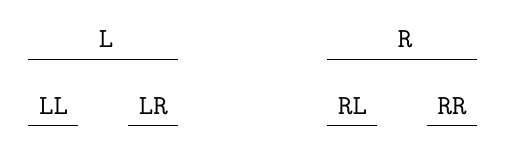
\begin{tikzpicture}[x=0.75pt,y=0.75pt,yscale=-0.8,xscale=0.8]
		%uncomment if require: \path (0,300); %set diagram left start at 0, and has height of 300

		\draw (170,120) -- (200,120);
		\draw (230,120) -- (260,120);
		\draw (350,120) -- (380,120);
		\draw (410,120) -- (440,120);
		\draw (170,80) -- (260,80);
		\draw (350,80) -- (440,80);
		\draw (211,61.4)  node [anchor=north west][inner sep=0.75pt] {$\mathtt{L}$};
		\draw (391,61.4)  node [anchor=north west][inner sep=0.75pt] {$\mathtt{R}$};
		\draw (175,101.4) node [anchor=north west][inner sep=0.75pt] {$\mathtt{LL}$};
		\draw (415,101.4) node [anchor=north west][inner sep=0.75pt] {$\mathtt{RR}$};
		\draw (235,101.4) node [anchor=north west][inner sep=0.75pt] {$\mathtt{LR}$};
		\draw (355,101.4) node [anchor=north west][inner sep=0.75pt] {$\mathtt{RL}$};
		\end{tikzpicture}
	\end{figure}
	\FloatBarrier
	
	As $C_k = \cup_{n=1}^{2^k}I_n^k$, at each subsequent step every interval $I_n^k$ is divided into two sub-intervals, namely \texttt{R} and \texttt{L}.\\	
	Let $x \in T = \cap_{k=1}^\infty C_k$. At step one $x$ can be either in \texttt{L} or in \texttt{R}. If we take $x \in \texttt{L}$, at step two $x$ can be $x \in \texttt{LL}$ or $x \in \texttt{LR}$.\\
	We continue tracing down the intervals where $x$ lies in each $C_k$, thus getting an unique, infinite sequence of \texttt{L} and \texttt{R}.\\
	Then we define a map $f: T \to E = \{\{s_k\}_{k \in \NN} : s_k = \texttt{L} \text{ or } \texttt{R} \quad \forall k\}$.
	
	We could prove that $E$ is uncountable and $f$ is bijective: we would have $|T| = |E|$ that prove our thesis.
	
	\textit{The set $E$ is uncountable:}\\ By contradiction, suppose that $E$ is countable; then we could assign a natural number to every element of $E$:
	$$E = \{ x^{(n)} = \{s_k^{(n)}\}_{k \in \NN} : n \in \NN\}.$$
	We construct a new sequence $x = \{t_n^{(n)}\}_{n \in \NN}$  with 
	\[t_n \coloneqq
	\begin{cases}
	\texttt{L} & \text{if } s_n^{(n)} = \texttt{R} \\
	\texttt{R} & \text{if } s_n^{(n)} = \texttt{L}
	\end{cases}\]
	Clearly $x \in E$, since it is made of \texttt{R} and \texttt{L}, but $t_n \neq s_n^{(n)}$ and thus $x \neq x^{(n)}$ for all $n$. Then $E$ is uncountable.
	
	\textit{The function $f$ is injective:}\\	Let $x,y \in T$ such that $f(x) = f(y)$.\\
	By construction for any $k$ we have that $x$ and $y$ belong to the same $I_n^k$.\\
	As 
	$$
	|I_n^k| 
	= \frac 1{3^k}
	$$ 
	and 
	$$
	|x-y| 
	\leq |I_n^k| 
	= \frac 1 {3^k} 
	\quad \forall k
	,
	$$
	we gain that $x=y$ and $f$ is injective.
	
	\textit{The function $f$ is surjective:}\\
	Let $\{s_k\}_k \in E$. We have to prove that there exists $x \in T$ such that $f(x) = \{s_k\}_k$.\\
	Fix $\{s_k\}_k$ and let $I_{n_k}^k$ be the interval identified by $\{s_k\}_k$ at each step $k$.\\
	In each $k$ we can take 
	$$
	y_k 
	\in I_{n_k}^k \cap T
	, \text{ with, by construction, }
	I_{n_{k+1}}^{k+1} 
	\subset I_{n_k}^k
	.
	$$
	We can assert that $\{y_k\}$ is a fundamental sequence, indeed we have:
	$$
	d_E(y_k, y_{k+1}) 
	< |I_{n_k}^k| 
	= \frac 1 {3^k} 
	\xrightarrow{k \to \infty}
	0
	.
	$$
	Moreover, $([0,1], d_E)$ is complete, indeed it is a closed subset of a complete metric space $(\RR, d_E)$, then $\{y_k\}$ is converging to an $x \in [0,1]$.\\
	As $T$ is compact, it is closed and sequentially closed, so $x \in T$.\\
	
	We have still to prove that $f(x) = \{s_k\}_k$.\\
	By contradiction suppose that there exists a sequence $\{t_k\}_k$ and a certain $\bar k$ for which $t_{\bar k} \neq s_{\bar k}$, and suppose that $f(x) = \{t_k\}_k$.\\
	Obviously $\{t_k\}_k \neq \{s_k\}_k$, indeed we have that for all $k > \bar k$ we have $t_k \neq s_k$.\\
	So $x \in I_{m_1}^{\bar k}$ (the interval represented by $\{t_k\}_k$), but $y_{\bar k}, y_{\bar k + 1}, \ldots$ belongs to $I_{m_2}^{\bar k}$ (represented by $\{s_k\}_k$).\\
	Then we have: 
	$$
	d_E(x, y_{\bar k + p}) 
	> \frac 1 {3^{\bar k}}
	\quad \forall p
	\text{ but }
	y_k 
	\to 
	x
	\text{ as }
	d(x, y_{k+p}) 
	\xrightarrow{p \to \infty}
	0
	.
	$$
	So we have a contradiction, then $f$ is bijective and this ends the proof.		
\end{proof}

\begin{prop}\label{Cantor-set-cardinalityofRR}
	The Cantor set has the same cardinality of $\RR$ and $[0,1]$.
\end{prop}

\paragraph{The generalized Cantor set} Similarly as before, it is construct by removing at each step not a third of the previous interval but a smaller, arbitrary quantity. What we will obtain is a non-zero-measure set which still have useful characteristics.

\begin{defn}
	The \emph{generalized Cantor set} $T$ is defined as follows.\\
	Fix $\eps \in (0, 1)$ and take $C_0^\eps = I_0^{\varepsilon, 0} = [0, 1]$. \\
	We build $C_1^\eps$ by erasing the open middle portion of size $\frac \eps 3$ from $I_0^{\varepsilon, 0}$, and $C_2^\eps$ by erasing the open middle portion of size $\frac {\eps^2} 9$ from $I_0^{\varepsilon, 1}$ and $I_1^{\varepsilon, 1}$, the intervals composing $C_1^\eps$.
	
	Now iterate the process: $C_k^\eps$ is constructed removing open middle portions of size $\left( \frac \eps 3 \right)^k$ from each interval $I_n^{\varepsilon, k-1}$ of $C_{k-1}^\eps$.
	
	The \emph{generalized Cantor set} is defined as:
	$$
		T_\eps 
		= \bigcap_{k=1}^\infty C_k^\eps
	.
	$$
\end{defn}

The generalized Cantor set has many properties analogues to the Cantor set, in particular holds the following propositions:
it is non-empty (\vref{Cantor-set-non-empty}), closed (\vref{Cantor-set-closed}), compact (\vref{Cantor-set-compact}), perfect (\vref{prop-cantor-set-perfect}), does not contains any interval (\vref{Cantor-set-not-contains-open-intervals}) and is uncountable (\vref{prop-cantor-set-uncountable}) with the same cardinality of $\RR$ (\vref{Cantor-set-cardinalityofRR}).\\
Anyway its measure is not zero, indeed it is easy to compute $|T_\eps|$:
$$
\left|T_\eps\right| 
= 1 - \frac \eps 3 - 2 \frac {\eps^2} 9 - \ldots
= 1 - \sum_{k=1}^{+\infty} 2^{k-1} \left( \frac \eps 3 \right)^k
= 1 - \frac 1 2 \sum_{k=1}^{+\infty} \left( \frac {2\eps} 3 \right)^k
= \frac{3(1 - \eps)}{3 - 2\eps} 
> 0
.
$$
You can still prove that $T_\eps$ does not contain any interval: start by computing $\left|I_{n,\eps}^{(k)}\right| \to 0$.

The characteristic function of $T_\eps$, $\Ind_{T_\eps}$ is Lebesgue-integrable:
$$\int_0^1 \Ind_{T_\eps} \, \de \mu = \left|T_\eps\right|.$$ 
Observe that it is not Riemann-integrable; you reader should prove it: the interior of $T_\eps$ is $\varnothing$, its measure is zero, the lower Riemann sum converges to 0, but $\left|T_\eps\right| > 0$, and thus the upper Riemann sum converges to $\left|T_\eps\right|$.

\paragraph{The Vitali--Cantor function} This function, also known as \textit{the devil's staircase}, present many properties in terms of continuity and derivability which make it a good counterexample in many situation. Its definition does not coincide with its construction. 

\begin{defn}\label{Vitali-Cantor-function}
	The \emph{Vitali--Cantor function}, is a function $f: [0, 1] \to [0, 1]$ such that:
	\begin{itemize}
		\item $f(0) = 0$ and $f(1) = 1$;
		\item $f$ is continuous and monotone non-decreasing;
		\item $f$ is derivable almost everywhere in $[0, 1]$, with $f' = 0$ almost everywhere in $[0, 1]$.
	\end{itemize}
\end{defn}

Such function can be obtained through a limit of the following series of function:
\begin{align*}
f_0(x) = & \ x\\[1 em]
f_1(x) = &
\begin{cases}
{\tfrac 3 2} x & \text{if } x \in [0, \tfrac 1 3] \\
{\tfrac 1 2} & \text{if } x \in (\tfrac 1 3, \tfrac 2 3) \\
{\tfrac 3 2} (x - \tfrac 1 3) & \text{if } x \in [\tfrac 2 3, 1] \\
\end{cases}\\[0.5 em]
= & \begin{cases}
\frac 1 2 & \text{if } x \in [0, 1] \setminus C_1 \\
\text{linear} & \text{if } x \in C_1
\end{cases} \\[0.5 em]
= & \int_0^x g_1(t) dt \qquad \text{with} \qquad g_1(t) = \frac 3 2 \Ind_{C_1}(t)\\[1 em]
f_2(x) = &
\begin{cases}
\frac 1 2 & \text{if } x \in [\frac 1 3, \frac 2 3] \\
\frac 1 4 & \text{if } x \in [\frac 1 9, \frac 2 9]  \\
\frac 3 4 & \text{if } x \in [\frac 7 9, \frac 8 9]  \\
\text{linear} & \text{if } x \in C_2
\end{cases} \\[0.3 em]
= & \int_0^x g_2(t) dt \qquad \text{with} \qquad g_2(t) = \left( \frac 3 2 \right)^2 \Ind_{C_2}(t)\\[0.5 em]
\vdots \ &\\[0.3 em]
f_k(x) = & \int_0^x g_k(t) dt \qquad \text{with} \qquad g_k(t) = \left( \frac 3 2 \right)^k \Ind_{C_k}(t)
\end{align*}

The limit of the sequence $\{f_k\}$ is the Vitali--Cantor function, we will prove this through the following propositions. Let's see its graph:
\begin{figure}[htpb]
	\centering
	% cfr. https://tex.stackexchange.com/questions/241622/plotting-the-cantor-function
	\tikzset{
	  if/.code n args=3{\pgfmathparse{#1}\ifnum\pgfmathresult=0
	    \pgfkeysalso{#3}\else\pgfkeysalso{#2}\fi},
	  lower cantor/.initial=.3333, upper cantor/.initial=.6667, y cantor/.initial=.5,
	  declare function={
	    cantor_l(\lowerBound,\upperBound)=
	      (\pgfkeysvalueof{/tikz/lower\space cantor})*(\upperBound-\lowerBound)+\lowerBound;
	    cantor_u(\lowerBound,\upperBound)=
	      (\pgfkeysvalueof{/tikz/upper\space cantor})*(\upperBound-\lowerBound)+\lowerBound;
	    cantor(\lowerBound,\upperBound)=% fun definition
	      (\pgfkeysvalueof{/tikz/y\space cantor})*(\upperBound-\lowerBound)+\lowerBound;},
	  cantor start/.style n args=5{%
	    insert path={(#1,#3)},
	    cantor={#1}{#2}{#3}{#4}{#5}{0},
	    insert path={to[every cantor edge/.try, cantor 1 edge/.try] (#2,#4)}},
	  cantor/.style n args=6{%
	    /utils/exec=%
	      \pgfmathsetmacro\lBx{cantor_l(#1,#2)}%
	      \pgfmathsetmacro\uBx{cantor_u(#1,#2)}%
	%      \pgfmathsetmacro\y{.5*(#3+#4)},% proper definition
	      \pgfmathsetmacro\y{cantor(#3,#4)},% fun
	    style/.expanded={
	      if={#6<#5}{cantor={#1}{\lBx}{#3}{\y}{#5}{#6+1}}{},
	      insert path={
	        to[every cantor edge/.try, cantor 1 edge/.try] (\lBx,\y)
	        to[every cantor edge/.try, cantor 2 edge/.try] (\uBx,\y)},
	      if={#6<#5}{cantor={\uBx}{#2}{\y}{#4}{#5}{#6+1}}{}}}}

	\foreach \level in {0,...,2}{
	\begin{tikzpicture}[line join=round] % cantor 1 edge/.style={move to}
	  \useasboundingbox[draw, scale=4, help lines]
	    (0,0) grid[xstep=1/9, ystep=.25] (1,1);
	  \draw[thick, cantor start={0}{4}{0}{4}{\level}{0}];
	\end{tikzpicture}}
	\caption{Construction of the Vitali--Cantor function.}
\end{figure}
\FloatBarrier
as we can see, it can be considered as a fractal.

\begin{prop}\label{prop-first-vitali}
	For any $k$ we have that $f_k(0) = 0$ and $f_k(1)=1$.
\end{prop}
\begin{proof}
	Considering the properties of the defined integral, as the integral domain is reduced to a point, we have $f_k(0) = 0$.
	The other result can be computed:
	$$
	f_k(1) 
	= \int_0^1 \left( \frac 3 2 \right)^k \Ind_{C_k}(t) \, \dt 
	= \left( \frac 3 2 \right)^k |C_k| 
	= 1
	.
	$$
\end{proof}

\begin{prop}\label{prop-second-vitali}
	For any $k$ we have that $f_k$ is monotonic increasing and Lipschitz-continuous.
\end{prop}
\begin{proof}
	Observe that for any $x < y$ we have:
	$$
	|f_k(y) - f_k(x)| 
	= \abs{\int_x^y g_k(t) \, \dt} 
	= \int_x^y g_k(t) \, \dt 
	\le \left( \frac 3 2 \right)^k \abs{y-x}
	.
	$$
	This fits the Lipschitz-continuity (see definition \vref{defn-lipschitz-continuity}) and shows that it is also bounded.
\end{proof}

\begin{prop}\label{prop-third-vitali}
	The sequence is piece-wise constant.\\
	In particular if  $x \in C_k\comp$, then $f_k(x) = f_{k+m}(x)$ for all $m \in \NN$, and precisely there exists $N_x \in \NN$ such that:
	$$
	f_k(x) 
	= f_{k+m}(x) 
	= \frac{N_x}{2^k} 
	\quad \forall m \in \NN
	.
	$$
\end{prop}
\begin{proof}
	First, we prove the equality. If $x \notin C_k = \bigcup_{n=1}^{2^k} I_n^k$, then there exist $N_x$ intervals $I_n^k$ such that $I_n^k \subset [0, x]$, and $(2^k-N_x)$ intervals $I_k^n$ such that $I_n^k \subset [x, 1]$, thus
	$$f_k(x)
	= \int_0^x \left( \frac 3 2 \right)^k \Ind_{C_k}(t) \, \dt
	= \left( \frac 3 2 \right)^k N_x |I_n^k|
	= \left( \frac 3 2 \right)^k N_x  \left( \frac 1 3 \right)^k
	= \frac{N_x}{2^k}$$
	
	Now we prove the value. If $x \notin C_k$, then $x \notin C_{k+1}$: since each interval $I_n^k$ produces two intervals $I_n^{k+1}$, when we have $N_x$ intervals $I_n^k \subset [0, x]$, then we also have $2N_x$ intervals $I_n^{k+1} \subset [0, x]$. Therefore:
	$$f_{k+1}(x) = \left( \frac 3 2 \right)^{k+1} \cdot 2N_x \cdot |I_n^{k+1}| = \frac{N_x}{2^k}.$$
	Thus $f_k(x) = f_{k+1}(x)$, and by induction $f_k(x) = f_{k+m}(x) \quad \forall m \in \NN$.
\end{proof}

\begin{prop}\label{prop-fourth-vitali}
	Each complementary of a set $C_k$ can be rewritten as an union of open sets, namely:
	$$
	C_k\comp 
	= \bigcup J_n^{(k)}
	,
	$$
	where $J_n^{(k)}$ are open.\\
	Moreover, if $x \neq y$ and $x, y$ are contained in the same $J_n^{(k)}$, then $f_k(x) = f_k(y)$.
\end{prop}
\begin{proof}
	Considering the previous proposition, this follows as $x, y \notin C_k$, and $N_x = N_y$.
\end{proof}

\begin{prop}\label{prop-fifth-vitali}
	The sequence $\{f_k\}$ is fundamental with respect to $d_\infty$.
	Moreover, the limit $f$ exists, $f(0) = 0$, $f(1) = 1$ and $f$ is monotonic increasing.
\end{prop}
\begin{proof}
	Take $x \in C_k\comp$. Then $f_{k+1}(x) = f_k(x)$.\\
	By continuity of $f_k$ and $f_{k+1}$ we have:
	$$
	f_{k+1}(x) 
	= f_k(x)
	\quad \forall x \in \widebar{C_k\comp}
	.
	$$
	Take now $x \in \left( \widebar{C_k\comp} \right)\comp =  \mathring{C_k}$ instead. Then $x \in \mathring{I_n^k} = (a_k, b_k)$: we have $f_{x+1}(a_k) = f_k(a_k)$ and $f_{k+1}(b_k) = f_k(b_k)$.
	
	Using the triangular inequality and the monotonicity of $f$:
	\begin{align*}
	|f_{k+1}(x) - f_k(x)|
	&= |f_{k+1}(x) - f_{k+1}(a_k) + f_{k+1}(a_k) - f_k(x)| \\
	&\le |f_{k+1}(x) - f_{k+1}(a_k)| + |f_k(x) - f_k(a_k)| \\
	&\le (f_{k+1}(b_k) - f_{k+1}(a_k)) + (f_k(b_k) - f_k(a_k)) \\
	&= 2 \cdot (f_k(b_k) - f_k(a_k))\\
	&= 2 \int_{a_k}^{b_k} g_k(t) \,\dt\\
	&= 2 \int_{a_k}^{b_k} \left( \frac 3 2 \right)^k \, \dt\\
	&= 2 \cdot \left( \frac 3 2 \right)^k \cdot \frac{1}{3^k}\\
	&= \frac{1}{2^{k-1}}
	\end{align*}
	And thus:
	\[
	d_\infty(f_{k+1}, f_{k}) 
	\le \frac{1}{2^k-1} 
	\xrightarrow{k \to +\infty} 0
	.
	\]
	Hence $\{ f_k \}$ is a fundamental sequence in $(\Cc^0([0, 1]), d_\infty)$, which is complete, and thus there exists
	$$
	f 
	\in \Cc^0([0, 1]):
	f_k 
	\xrightarrow{d_\infty} f
	.
	$$
	Thus $f(0) = 0$, $f(1) = 1$ and $f$ is monotonic increasing.
\end{proof}

\begin{prop}\label{prop-sixth-vitali}
	The function $f$ is differentiable almost everywhere; where that is possible we have $f'(x) = 0$.
\end{prop}
\begin{proof}
	Let $x \notin T$. Then there exists $k \in \NN$ such that $x \notin C_k$.\\
	But $C_k\comp$ is open, and hence there exists $\eps > 0$ such that $(x - \eps, x + \eps) \in C_k\comp$. Therefore, by what we proved in the previous points (\vref{prop-third-vitali} and \vref{prop-fourth-vitali}), we have that 
	$$
	f_{k+m}(y) 
	= \frac{N_x}{2^k}
	\quad \forall y \in (x - \eps, x + \eps) 
	\quad \forall m \in \NN
	.
	$$
	
	As $m \to + \infty$, we obtain 
	$$
	f(y) 
	= \frac{N_x}{2^k} 
	\quad \forall y \in (x - \eps, x + \eps)
	.
	$$
	This means that $f$ is constant in a neighborhood of $x$, and thus it is differentiable in $x \in T\comp$, with $f'(x) = 0$. Observe that the function $f$ is not differentiable only in $T$: but as $|T| = 0$ we have that $f$ is differentiable almost everywhere.
\end{proof} 

%\input{sections/1_E_1_Cardinalities}

%%%%%%%%%%%%%%%%%%%%%%%%%%%%%%%%%%%%%%%%%%%%%%%%%%%%%%%%
\newpage
\section{Real Analysis}
Now that we have introduced some fundamental notions about set theory and topolgy, we can begin our study of Real Analysis, which is a branch of mathematical analysis that studies real numbers and the most common operations we can do with them: sequences, series, functions, integration.\\
This raises some meaningful questions: how are they defined from a rigorous point of view? Which are their properties? Are there some operations that cannot be done for certain reasons? Which characterizations can we find to connect these structures?\\
In this part we will first introduce measure theory, which as abstract as it may seem, it is essential to define the powerful Lebesgue integral later on. Measure theory also does some \textit{dotting the i's and crossing the t's} on something that the reader may have seen many times in previous courses: probability. Some concepts that maybe did not add up before, now will make sense. We will also explore in a meaningful way the concept of non-measurable sets, which is way more non-trivial than measurable sets.\\
Then, starting from a formal definition of integration according to Lebesgue, we will see some relevant theorems and properties, useful both in pratical and theoretic fields.\\
We will see the two fundamental theorems of calculus, something that the reader may have also seen in a simplified form in previous courses. To this end, we will explore new definitions of continuity.\\
At last, we will give some definitions and useful theorems to deal with measures defined in product spaces.

\newpage
\subsection{Measure theory}
%!TEX root = ../main.tex
Here we try to find a way to measure sets. Considering for instance a non-empty set $\Omega$, how can we define a set function $\mu : \Pc(\Omega) \to [0, +\infty]$ which is interpretable as a \emph{measure} of the set $\Omega$? Are there some properties required?

Two reasonable properties for such function are: 
$$
	\mu(\varnothing) 
	= 0, 
	\quad \mu(A \cup B) 
	= \mu(A) + \mu(B)
	\quad \text{ if } 
	\quad A \cap B 
	= \varnothing
.
$$
Does a function with those properties exist?

\subsubsection{Measurable spaces}
Our first step is to define a good environment in which we can have all the tools we need: let's define on which kind of sets we can search for such measure.

\begin{defn}
  Consider a non-empty set $\Omega$.
  The family of subsets $\mm \subseteq \Pc(\Omega)$ is a \emph{$\sigma$-algebra} of $\Omega$ if:
  \begin{itemize}
    \item the \emph{empty set is included}:
    	$$
    		\varnothing \in \mm
    	;
    	$$
    \item it is \emph{closed with respect to complements}:
    	$$
    		E \in \mm 
    		\implies E\comp \in \mm
    	;
    	$$
    \item it is \emph{closed with respect to countable unions}:
     	$$
     		\{ E_i \}_{i \in \NN} \subseteq \mm 
     		\implies \bigcup_{i \in \NN} \, E_i \in \mm
     	.
     	$$
  \end{itemize}
\end{defn}
It can be easily shown from the definition, that also $\Omega$ itself belongs to the $\sigma$-algebra and, by using the De Morgan's laws, that $\mm$ is closed with respect to countable intersections: 
$$
	\forall \{E_j\}_{j\in \NN} \in \mm 
	\qquad \bigcap_{j \in \NN} \, E_j 
	= \bigcap_{j \in \NN} \, (E_j\comp)\comp 
	=\left( \bigcup_{j \in \NN} \, E_j\comp \right)\comp 
	\in \mm
.
$$
Similarly it can be proved that the difference of sets belonging to the $\sigma$-algebra itself belongs to the $\sigma$-algebra.

The power set $\Pc(\Omega)$ is known to be the trivial $\sigma$-algebra.

This allow us to find the ideal environment for a measure:

\begin{defn}
  Let $\Omega \neq \varnothing$ and $\mm \subseteq \Pc(\Omega)$ be a $\sigma$-algebra.\\
  Then $(\Omega, \mm)$ is a \emph{measurable space}.
\end{defn}

It is easy to show that the intersection of $\sigma$-algebras is still a $\sigma$-algebra.

To many purposes is useful to consider the ``smallest'' $\sigma$-algebra containing a given family of subsets of $\Omega$. The following definition formalize this concept.
\begin{defn}
	Let $\Ec \in \Pc(\Omega)$.\\
	The \emph{$\sigma$-algebra generated by $\Ec$}, written as $\sca{\Ec}$, is defined as the intersection of all the $\sigma$-algebras containing $\Ec$.
  \end{defn}
It's easy to prove that this definition is well-posed, to do that, show that the intersection of those $\sigma$-algebras itself is a $\sigma$-algebra. Furthermore, it's easy to show that such $\sigma$-algebra is actually the smallest.

\begin{exer}
  Let $\Omega \neq \varnothing$.\\
  Consider $\Ec = \{ E_i \}_{i=1,\ldots,N}$ as a partition of $\Omega$: prove that $\sca{\Ec}$ has $2^N$ elements.
\end{exer}

Recalling the concepts of open sets and topological spaces (see definition \vref{topological-spaces}), here is presented a special $\sigma$-algebra which has been defined with a special name due to its relevance.
\begin{defn}
  Let $(X, \tau)$ be a topological space with $X \neq \varnothing$. \\
  We call \emph{Borel $\sigma$-algebra}, denoted by $\Bc(X)$, the $\sigma$-algebra generated by open sets.\\
  All the set that it contains are called \emph{Borel sets}.
\end{defn}

Here some general category of sets which belongs to the Borel $\sigma$-algebra. 
\begin{defn}\label{F-sigma-G-delta}
	We call \emph{$F_\sigma$ sets} every countable union of closed sets.\\
	We call \emph{$G_\delta$ sets} every countable intersection of open sets. \footnotemark{}
\end{defn}
\footnotetext{Felix Hausdorff (1868 - 1942) adopted this convection; \textit{F} is for the French word ``fermé'' which means closed, while $\sigma$ is for ``somme'' which means sum (union) in the same language; on the other hand, \textit{G} is for the German word ``Gebiet'' meaning area or neighbourhood, indicating open set, and $\delta$ is for ``Durchschnitt'' which means intersection.}

Open and closed sets, $F_\sigma$ sets and countable intersections of $F_\sigma$ sets, $G_\delta$ sets and countable unions of $G_\delta$ sets all belongs to the Borel $\sigma$-algebra.

%!TEX root = ../main.tex
\subsubsection{Measurable functions}

We have provide a definition for measurable spaces, but, yes, we still don't know how to measure them. Before that we'll discuss the concept of measurability for functions. The first steps will not involves any kind of function, but we will focus on an easily manageable case. It will be easy to extend those results to the general case.

\begin{defn}
  	Let $(X, \mm)$ be a measurable space, and $(Y, \tau)$ be a topological space. \\
  	We say that $f: X \to Y$ is a \emph{measurable function} if the preimage of any open set is measurable, namely:
  	$$
  		f^{-1}(A) \in \mm 
  		\quad \text{for all } A \in \tau
  	.
  	$$
\end{defn}

Observe that a function defined on two topological spaces, namely $f:(X, \tau_X) \to (Y, \tau_Y)$, if it maps open sets into open sets then it is $\Bc$-measurable with respect to the measurable space $(X, \Bc(X))$. Indeed, for every open set $A \in \tau$, $f^{-1}(A)$ is open in $X$ by definition, and thus $f^{-1}(A) \in \Bc(X)$.

\begin{theo}[Composition of a measurable function with a continuous one]
	Let $f:\; (\Omega, \mm) \to (X, \tau_X)$ be a measurable function and $g:\; (X, \tau_X) \to (Y, \tau_Y)$ be a continuous function.\\
	Then $g \circ f:\; \left(\Omega,\mm \right)\to \left(Y,\tau_Y\right)$ is measurable.
\end{theo}
As we said in the previous remark, $g$ is not only continuous but also $\Bc(X)$-measurable. Here we prove this case, which is more general with respect to the theorem.
\begin{proof}
	Let $A \subset Y$ be an open set, then $g^{-1}\left(A\right)\in \Bc\left(X\right)$. Now let $B \subset X$ be open, and $f^{-1}(B) \in \mm$.
	
	As $\Bc(X)$ is generated by all the open sets in $X$ and is closed with respect to union and complement, $f^{-1}(g^{-1}(A)) \in \mm$ and this means that $g\circ f$ is $\mm$-measurable (in case $A = \varnothing$ we have $g\circ f (A) = \varnothing \in \mm$) .
\end{proof}

If $f$ and $g$ are just measurable, then $g \circ f$ is not necessarily measurable, even if $f$ is continuous.

\paragraph{Measurable functions in $\RR$}There are some important results that holds when working in $\RR$. First, the previous theorem can be extended to the multi dimensional case.
\begin{theo}\label{multiple-measurable-function-composed-contiunuous} 
	Let $\left(u,v\right) : \left(\Omega,\mm\right)\to\RR^2$ be $\mm$-measurable. \\
	Moreover, let $\Phi : \ \RR^2 \to \left(X,\tau \right)$ be continuous.
	
	Then $h=\Phi\left(u,v\right):\ \left(\Omega,\mm\right)\to \left(X,\tau\right)$ is $\mm$-measurable.
\end{theo}
\begin{proof}
	Let $A \subseteq X$ be open. Then $\Phi^{-1}(A)\subseteq \RR^2$ is open. \\
	Thanks to theorem \vref{open-set-RR-intervals}, we have that $\Phi^{-1}(A) = \bigcup_{i \in \NN} I_{i}\times J_{i}$ where $I_{i},\ J_{i} \subset \RR$ are intervals. \\
	Finally, observe that $h^{-1}\left(I_{i}\times J_{i}\right)=u^{-1}\left(I_{i}\right)\cap v^{-1}\left(J_{i}\right) \in \mm$.
\end{proof} 
This theorem has several implications: if $u,v:\left(\Omega,\mm\right)\to\RR^2$ are measurable, than $u\pm v$, $uv$, $|u|$, $u^+$, $u_-$ and other elementary operation with these functions returns $\mm$-measurable functions.

The following proposition shows a topological property of the set $\RR$, it will turn useful in many fields.

\begin{theo} \label{open-set-RR-intervals}
	Every open set $\Omega \in \RR$ can be written in a unique way as countable union of mutually disjoint intervals, namely: $$\Omega = \bigcup_{j=1}^{\infty} I_j \qquad I_j=\left(a_j,b_j\right).$$
	
	Every open set $\Omega \in \RR^N$, with $n>1$, can be written in a unique way as countable union of $n$ intervals,namely:
	$$\Omega = \bigcup_{j=1}^{\infty} I_j \qquad I_j=\left(a_j^1,b_j^1\right)\times\left(a_j^2,b_j^2\right)\times\cdots\times\left(a_j^n,b_j^n\right).$$
\end{theo}
\begin{proof}
	\textit{Step 1. The intervals are well defined}:\\
	First, consider $x \in \Omega$: we need to build the largest open interval $I_x\subset \Omega$ containing $x$.\\
	We define $I_x = (a_x,b_x)$ where:
	$$ 
		a_x 
		\coloneqq \inf \{a < x: (a,x) \subset \Omega \} \ 
		\text{ and } \ b_x \coloneqq \sup \{b>x:(x,b) \subset \Omega \}
	;
	$$
	notice that $I_x \neq \varnothing$, $a_x \neq x$  and $b_x \neq x$ since $\Omega$ is open and $x \in \Omega$.\\
	Certainly we have that $a_x \in [-\infty, x)$ and $b_x \in (x, +\infty]$.\\
	Moreover, we show that $I_x \in \Omega$; let $w \in I_x$, without loss of generality we assume that $x < w < b_x$. Then by the definition of $b_x$, it exists $b > w$ such that $(x,b) \in \Omega$: then $w \in \Omega$.
	
	\textit{Step 2. The set is the union of the intervals}:\\
	Consider the collection of open intervals $\{I_x\}_{x\in \Omega}$. Since each $x\in \Omega$ and $x \in i_x \subseteq \Omega$, then 
	$$
		\Omega 
		= \bigcup_{x\in \Omega} I_x
	.
	$$
	Here we have two problems: first, the family $\{I_x\}_{x\in \Omega}$ may not be disjoint; second the same family can be uncountable.
	
	\textit{Step 3. The family of intervals is disjoint}:\\
	To solve the first problem we have to prove that if $x,y \in \Omega$, then either $I_x = I_y$ or $I_x \cap I_y = \varnothing$.\\
	If $I_x \cap I_y \neq \varnothing$ then $I_x \cup I_y$ is still an open interval, and it contains both $x$ and $y$, and it is a subset of $\Omega$.\\
	Since $I_x$, as we proved before, is the largest open interval in $\Omega$ containing $x$, we have:
	$$
		I_x \supseteq I_x \cap I_y \supseteq I_x 
		\implies I_x = I_x \cup I_y
	.
	$$
	Similarly we can show that $I_x = I_y$.
	
	\textit{Step 4. The family of intervals is countable}:\\
	Since for any $x\in \Omega$ there exists a rational number $q \in I_x \subseteq \Omega$, and we have that $I_x \cap I_q \neq \varnothing$, hence $I_x = I_q$.\\
	This means that: $$\Omega = \bigcup_{x\in\Omega} I_x = \bigcup_{q \in \QQ \cap \Omega} I_q$$
	as $\QQ$ is countable, then $\Omega \cap \QQ$ is countable as well, hence the thesis.	
\end{proof}
This proof can be extended to $\RR^N$ case.

\begin{prop}
	Every open set $\Omega \subset \RR^N$ can be written as a countable union of closed, disjoint cubes, namely:
	$$ \Omega = \bigcup_{j = 1}^{\infty} R_j$$
	where
	$$R_j = [a_j^1,b_j^1]\times[a_j^2,b_j^2]\times\cdots\times[a_j^n,b_j^n]$$
	with
	$$a_j^i < b_j ^i \ \forall i \text{ and } \mathring R_i \cap \mathring R_k = \varnothing \ k \neq i.$$ 
\end{prop}
Observe that $R_j$ must be almost disjoints.


This last results is about the Borel $\sigma$-algebras of $\RR$ and $\RR^\star$; they don't need the entire topology to be generated. 
\begin{theo}\label{borel-sigma-algebra-of-rr}
	The Borel $\sigma$-algebra of $\RR$ and $\RR^\star$ are defined as follows:
	$$\Bc(\RR)=\sca{\{\left(a,b\right)\}_{a,b \in \RR}} \qquad \Bc(\RR^\star )=\sca{\{\left(a,+\infty\right]\}_{a\in\RR}}.$$
\end{theo}
\begin{proof}
	\textit{Proof of the generator sets of $\Bc(\RR)$}:\\
	This first statement follows from theorem \vref{open-set-RR-intervals}.
	
	\textit{Proof of the generator sets of $\Bc(\RR^\star)$}:\\
	For the second one, let us consider the set $\left(a, +\infty\right]$, which is open $\forall a \in \RR$. So we have that:
	$$\Bc(\RR^\star) \supseteq \sca{\{\left(a,+\infty\right]_{a \in \RR}\}} \eqqcolon \mm.$$
	Now we want to prove that $\Bc(\RR^\star) \subseteq \mm$, by checking that the sets $[-\infty, a]$, $(a, b)$, $(b, +\infty]$ are contained in $\mm$ for all $a$, $b$:
	\begin{align*}
	[-\infty, a] &= (a, +\infty]\comp \in \mm \\
	\left[-\infty,a\right) &= \bigcup_{n=1}^\infty \left(-\infty, a - \frac 1 n \right] \in \mm \\
	(a,b) &= \left[-\infty,b\right) \cap \left(a,+\infty\right] \in \mm
	\end{align*}
	The sets $[-\infty, a]$, $(a, b)$, $(b, +\infty]$ form a base for the topology of $\RR^\star$, and thus $\mm \supseteq \Bc(\RR^\star)$.\\
	That proves that $\Bc(\RR^\star) \subseteq \mm$.
\end{proof}


Indeed, those structures are generated as follows: 
	$$\Bc(\RR)=\sca{\{\left(a,b\right)\}_{a,b \in \RR}} \qquad \Bc(\RR^\star )=\sca{\{\left(a,+\infty\right]\}_{a\in\RR}}$$
See proposition \vref{borel-sigma-algebra-of-rr} for the proof of this result.


\paragraph{Measurability for sequence of functions} Now we pose the following problem: having a sequence of measurable function which converges to a limit function, is that function measurable? Before look at these results, recall the notions of \textit{liminf} and \textit{limsup} explained in the appendix.

\begin{theo} \label{lim-are-measurable}
	Let $f_n:\left(\Omega,\mm\right)\to \RR^\star$ be $\mm$-measurable functions for all $n \in \NN$. \\
	Then $\sup f_n$, $\inf f_n$, $\limsup f_n$,  $\liminf f_n$ are all $\mm$-measurable.
\end{theo}
\begin{proof}
	\textit{Step 1. Inferior and superior}:\\ Consider $g(x) \coloneqq \sup f_n(x)$:
	\begin{align*}
	g^{-1}((a, +\infty])
	& = \{ x \in \RR^\star \ |\ \sup f_n(x) > a \}\\
	& = \{ x \in \RR^\star \ |\ \exists \, n : f_n(x) > a \} \\
	& = \{ x \in \RR^\star \ |\ \exists \, n : x \in f_n^{-1}((a, +\infty]) \} \\
	& = \bigcup_{n\in\NN}f_n^{-1}\left(\left(a,+\infty\right]\right)\\
	& \in\mm
	.
	\end{align*}

	We need to prove the measurability only on $(a, +\infty]$, the remaining comes by properties of $\sigma$-algebra and topology; indeed, all the generators of the topology $\tau_C^\star$ have a counterimage in $\mm$.
	
	Consider now $g(x) \coloneqq \inf f_n(x)$. Arguing as before we get: $g^{-1}\left(\left[-\infty,a\right)\right) = \bigcup_{n\in\NN}f_n^{-1}\left(\left[-\infty,a\right)\right)\in\mm$.
	
	\textit{Step 2. Liminf and limsup}:\\
	Then consider $g(x) \coloneqq \limsup f_n(x) = \inf_{n\ge 0}\left(\sup_{k\geq n} f_k(x) \right)$.
	In the previous lines we have shown that $\sup_{k \geq 0} f_k$ is measurable, and so is the function $h_n = \sup_{k \geq n} f_k$, for any $n \in \NN$; the infimum of such sequence, which is $\inf h_n \left(\sup_{k \geq n} f_k\right) = g(x)$, is also measurable as we shown before.
	
	We can argue in a similar way for $\liminf f_n(x)$ and conclude the proof.
\end{proof}

\paragraph{Simple functions} Let consider a simple kind of functions for which is easy to find a measure. Those function will be the prototype of functions in general and though them we will extend their measure to all the measurable functions.

\begin{defn}\label{simple-function}
	Let $\left(\Omega,\mm\right)$ be a measurable space $\left(\Omega \neq \varnothing\right)$.\\
	We say that $s:\Omega \to \RR$ is a \emph{simple function} if it has the following form: $$s(t)=\sum_{n=1}^N a_n\Ind_{E_n}(t)$$
	where $a_j \in \RR$ and $\{E_j\}_{j=1}^N$ is a partition of $\Omega$ made of measurable sets.
\end{defn}

The set function $\Ind_{E}$ the indicator function.

\begin{exam}\label{ex:simple-functions}
	The function: $s(t)=\Ind_{[-\infty,2)}(t)+3\Ind_{[2,3]}(t)-\Ind_{(3,+\infty)}(t)$ is a simple function.
\end{exam}

\begin{figure}[htpb]
	\centering
	\tikzset{every picture/.style={line width=0.75pt}} %set default line width to 0.75pt        

	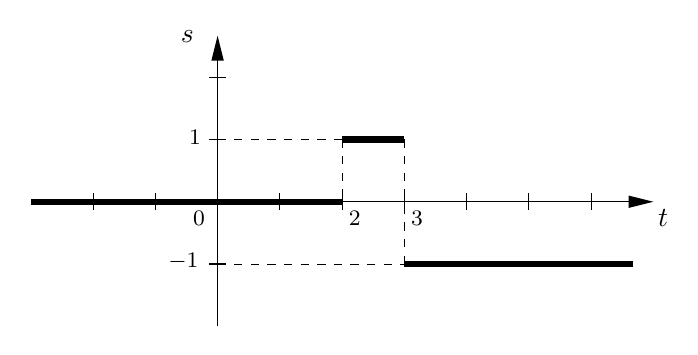
\begin{tikzpicture}[x=0.75pt,y=0.75pt,yscale=-1,xscale=1]
	\draw (80,90) -- (378,90) (110,86) -- (110,94)(140,86) -- (140,94)(170,86) -- (170,94)(200,86) -- (200,94)(230,86) -- (230,94)(260,86) -- (260,94)(290,86) -- (290,94)(320,86) -- (320,94)(350,86) -- (350,94) ;
	\draw [shift={(380,90)}, rotate = 180] [fill={rgb, 255:red, 0; green, 0; blue, 0 }  ][line width=0.08]  [draw opacity=0] (12,-3) -- (0,0) -- (12,3) -- cycle    ;
	\draw (170,150) -- (170,12) (166,120) -- (174,120)(166,90) -- (174,90)(166,60) -- (174,60)(166,30) -- (174,30) ;
	\draw [shift={(170,10)}, rotate = 90] [fill={rgb, 255:red, 0; green, 0; blue, 0 }  ][line width=0.08]  [draw opacity=0] (12,-3) -- (0,0) -- (12,3) -- cycle    ;
	\draw [line width=2.25]    (80,90) -- (230,90) ;
	\draw [dashed, very thin]  (230,60) -- (230,90) ;
	\draw [line width=2.25]    (230,60) -- (260,60) ;
	\draw [line width=2.25]    (260,120) -- (370,120) ;
	\draw [dashed, very thin]  (260,60) -- (260,120) ;
	\draw [dashed, very thin]  (170,60) -- (230,60) ;
	\draw [dashed, very thin]  (170,120) -- (260,120) ;

	\draw (157,93.4) node [anchor=north west][inner sep=0.75pt]  [font=\footnotesize]  {$0$};
	\draw (232,93.4) node [anchor=north west][inner sep=0.75pt]  [font=\footnotesize]  {$2$};
	\draw (155,54.4) node [anchor=north west][inner sep=0.75pt]  [font=\footnotesize]  {$1$};
	\draw (262,93.4) node [anchor=north west][inner sep=0.75pt]  [font=\footnotesize]  {$3$};
	\draw (145,113.4) node [anchor=north west][inner sep=0.75pt]  [font=\footnotesize]  {$-1$};
	\draw (151,6.4) node [anchor=north west][inner sep=0.75pt]  [font=\normalsize]  {$s$};
	\draw (381,92.4) node [anchor=north west][inner sep=0.75pt]  [font=\normalsize]  {$t$};
	\end{tikzpicture}
	\caption{Plot of the function of example \vref{ex:simple-functions}.}
\end{figure}
\FloatBarrier

\begin{theo}
	Let $(\Omega,\mm)$ be a measurable space, with $\Omega \neq \varnothing$.\\
	For any function $f:(\Omega,\mm) \to \left[0,+\infty\right]$, $\mm$-measurable, there exists a sequence of simple functions 
	$$
		\{s_n\}_{n\in \NN}: 
		\ (\Omega,\mm)\to\left[0,+\infty\right]
	$$
	such that:
	\begin{itemize}
		\item the sequence is monotone: 
			$$
				s_n(t) \leq s_{n+1}(t)
				\quad \forall t\in \Omega 
				\quad \forall n\in\NN
			;
			$$
		\item the sequence is dominated: 
			$$
				0 \leq s_n(t) \leq f(t)
				\quad \forall t \in \Omega 
				\quad \forall n\in\NN
			;
			$$
		\item the sequence converges point-wise: 
			$$
				\lim\limits_{n \to + \infty} s_n(t) = f(t) 
				\quad \forall t\in \Omega
			.
			$$
	\end{itemize}
	Moreover, if the function is bounded, namely there exists $M>0$ such that $f(t) < M$ for any $t \in \Omega$, the sequence converges uniformly to $f$ in $\Omega$.
\end{theo}

Notice that $[0,+\infty]$ is a topological space with the topology inducted by $(\RR^\star, \tau_C^\star)$.

The following is a constructive proof in which the sequence object of the theorem is built.

\begin{proof}
	Let $n \in \NN_0$, split $\left[0,n\right)$ in $k=n2^n$ intervals $\left[a_j,b_j\right)$ of length $2^{-n}$.
	
	Take $E_0=f^{-1}(\left[n,+\infty\right])$ and $E_j=f^{-1}([a_j,b_j])$, which are $\mm$-measurable.\\
	%\missingfigure{$E_j=f^{-1}([a_j,b_j])$}
	\begin{figure}[htpb]
		\centering
		\tikzset{every picture/.style={line width=0.75pt}} %set default line width to 0.75pt        

		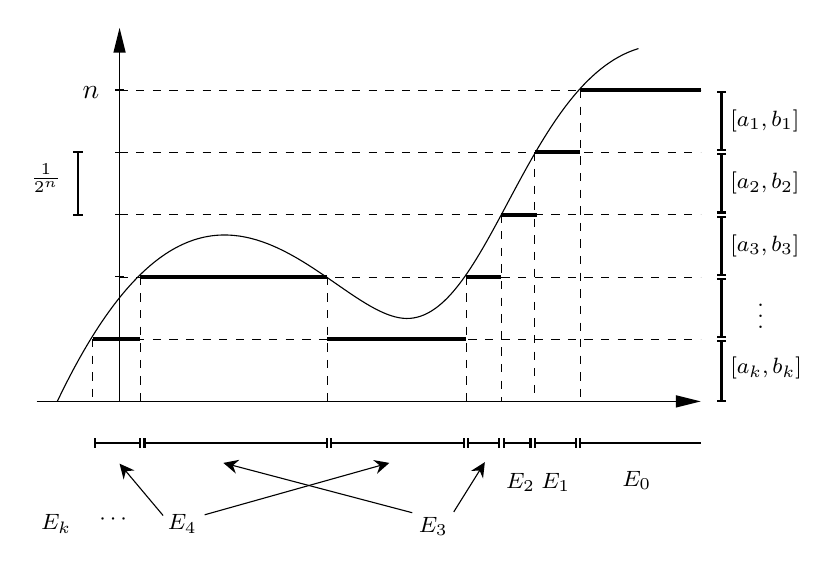
\begin{tikzpicture}[x=0.75pt,y=0.75pt,yscale=-1,xscale=1]
		%uncomment if require: \path (0,303); %set diagram left start at 0, and has height of 303

		\draw    (130,210) .. controls (204,55) and (262,173) .. (300,170) .. controls (338,167) and (357,56) .. (410,40) ;
		\draw [line width=0.75]  [dashed, very thin]  (160,60) -- (440,60) ;
		\draw [line width=0.75]  [dashed, very thin]  (160,90) -- (440,90) ;
		\draw [line width=0.75]  [dashed, very thin]  (160,120) -- (440,120) ;
		\draw  [dashed, very thin]  (160,150) -- (440,150) ;
		\draw  [dashed, very thin]  (160,180) -- (440,180) ;
		\draw  [dashed, very thin]  (170,150) -- (170,210) ;
		\draw  [dashed, very thin]  (260,150) -- (260,210) ;
		\draw  [dashed, very thin]  (327,150) -- (327,210) ;
		\draw  [dashed, very thin]  (344,120) -- (344,210) ;
		\draw  [dashed, very thin]  (360,90) -- (360,210) ;
		\draw  [dashed, very thin]  (382,60) -- (382,210) ;
		\draw  [dashed, very thin]  (147,180) -- (147,210) ;
		\draw [line width=1.5]    (147,180) -- (170,180) ;
		\draw [line width=1.5]    (170,150) -- (260,150) ;
		\draw [line width=1.5]    (327,150) -- (344,150) ;
		\draw [line width=1.5]    (344,120) -- (361,120) ;
		\draw [line width=1.5]    (360,90) -- (382,90) ;
		\draw [line width=1.5]    (382,60) -- (440,60) ;
		\draw [line width=1.5]    (260,180) -- (327,180) ;
		\draw [line width=0.75]    (382,230) -- (440,230) ;
		\draw [shift={(382,230)}, rotate = 180] [color={rgb, 255:red, 0; green, 0; blue, 0 }  ][line width=0.75]    (0,2.24) -- (0,-2.24)   ;
		\draw [line width=0.75]    (360,230) -- (380,230) ;
		\draw [shift={(380,230)}, rotate = 180] [color={rgb, 255:red, 0; green, 0; blue, 0 }  ][line width=0.75]    (0,2.24) -- (0,-2.24)   ;
		\draw [shift={(360,230)}, rotate = 180] [color={rgb, 255:red, 0; green, 0; blue, 0 }  ][line width=0.75]    (0,2.24) -- (0,-2.24)   ;
		\draw [line width=0.75]    (345,230) -- (358,230) ;
		\draw [shift={(358,230)}, rotate = 180] [color={rgb, 255:red, 0; green, 0; blue, 0 }  ][line width=0.75]    (0,2.24) -- (0,-2.24)   ;
		\draw [shift={(345,230)}, rotate = 180] [color={rgb, 255:red, 0; green, 0; blue, 0 }  ][line width=0.75]    (0,2.24) -- (0,-2.24)   ;
		\draw [line width=0.75]    (328,230) -- (343,230) ;
		\draw [shift={(343,230)}, rotate = 180] [color={rgb, 255:red, 0; green, 0; blue, 0 }  ][line width=0.75]    (0,2.24) -- (0,-2.24)   ;
		\draw [shift={(328,230)}, rotate = 180] [color={rgb, 255:red, 0; green, 0; blue, 0 }  ][line width=0.75]    (0,2.24) -- (0,-2.24)   ;
		\draw [line width=0.75]    (172,230) -- (260,230) ;
		\draw [shift={(260,230)}, rotate = 180] [color={rgb, 255:red, 0; green, 0; blue, 0 }  ][line width=0.75]    (0,2.24) -- (0,-2.24)   ;
		\draw [shift={(172,230)}, rotate = 180] [color={rgb, 255:red, 0; green, 0; blue, 0 }  ][line width=0.75]    (0,2.24) -- (0,-2.24)   ;
		\draw [line width=0.75]    (262,230) -- (326,230) ;
		\draw [shift={(326,230)}, rotate = 180] [color={rgb, 255:red, 0; green, 0; blue, 0 }  ][line width=0.75]    (0,2.24) -- (0,-2.24)   ;
		\draw [shift={(262,230)}, rotate = 180] [color={rgb, 255:red, 0; green, 0; blue, 0 }  ][line width=0.75]    (0,2.24) -- (0,-2.24)   ;
		\draw [line width=0.75]    (148,230) -- (170,230) ;
		\draw [shift={(170,230)}, rotate = 180] [color={rgb, 255:red, 0; green, 0; blue, 0 }  ][line width=0.75]    (0,2.24) -- (0,-2.24)   ;
		\draw [shift={(148,230)}, rotate = 180] [color={rgb, 255:red, 0; green, 0; blue, 0 }  ][line width=0.75]    (0,2.24) -- (0,-2.24)   ;
		\draw [line width=0.75]    (450,61) -- (450,89) ;
		\draw [shift={(450,89)}, rotate = 270] [color={rgb, 255:red, 0; green, 0; blue, 0 }  ][line width=0.75]    (0,2.24) -- (0,-2.24)   ;
		\draw [shift={(450,61)}, rotate = 270] [color={rgb, 255:red, 0; green, 0; blue, 0 }  ][line width=0.75]    (0,2.24) -- (0,-2.24)   ;
		\draw [line width=0.75]    (450,91) -- (450,119) ;
		\draw [shift={(450,119)}, rotate = 270] [color={rgb, 255:red, 0; green, 0; blue, 0 }  ][line width=0.75]    (0,2.24) -- (0,-2.24)   ;
		\draw [shift={(450,91)}, rotate = 270] [color={rgb, 255:red, 0; green, 0; blue, 0 }  ][line width=0.75]    (0,2.24) -- (0,-2.24)   ;
		\draw [line width=0.75]    (450,121) -- (450,149) ;
		\draw [shift={(450,149)}, rotate = 270] [color={rgb, 255:red, 0; green, 0; blue, 0 }  ][line width=0.75]    (0,2.24) -- (0,-2.24)   ;
		\draw [shift={(450,121)}, rotate = 270] [color={rgb, 255:red, 0; green, 0; blue, 0 }  ][line width=0.75]    (0,2.24) -- (0,-2.24)   ;
		\draw [line width=0.75]    (450,151) -- (450,179) ;
		\draw [shift={(450,179)}, rotate = 270] [color={rgb, 255:red, 0; green, 0; blue, 0 }  ][line width=0.75]    (0,2.24) -- (0,-2.24)   ;
		\draw [shift={(450,151)}, rotate = 270] [color={rgb, 255:red, 0; green, 0; blue, 0 }  ][line width=0.75]    (0,2.24) -- (0,-2.24)   ;
		\draw [line width=0.75]    (450,181) -- (450,210) ;
		\draw [shift={(450,210)}, rotate = 270] [color={rgb, 255:red, 0; green, 0; blue, 0 }  ][line width=0.75]    (0,2.24) -- (0,-2.24)   ;
		\draw [shift={(450,181)}, rotate = 270] [color={rgb, 255:red, 0; green, 0; blue, 0 }  ][line width=0.75]    (0,2.24) -- (0,-2.24)   ;
		\draw [line width=0.75]    (140,90) -- (140,120) ;
		\draw [shift={(140,120)}, rotate = 270] [color={rgb, 255:red, 0; green, 0; blue, 0 }  ][line width=0.75]    (0,2.24) -- (0,-2.24)   ;
		\draw [shift={(140,90)}, rotate = 270] [color={rgb, 255:red, 0; green, 0; blue, 0 }  ][line width=0.75]    (0,2.24) -- (0,-2.24)   ;
		\draw    (181,265) -- (161.93,242.3) ;
		\draw [shift={(160,240)}, rotate = 49.97] [fill={rgb, 255:red, 0; green, 0; blue, 0 }  ][line width=0.08]  [draw opacity=0] (7.14,-3.43) -- (0,0) -- (7.14,3.43) -- (4.74,0) -- cycle    ;
		\draw    (201,264.64) -- (287.11,240.45) ;
		\draw [shift={(290,239.64)}, rotate = 164.31] [fill={rgb, 255:red, 0; green, 0; blue, 0 }  ][line width=0.08]  [draw opacity=0] (7.14,-3.43) -- (0,0) -- (7.14,3.43) -- (4.74,0) -- cycle    ;
		\draw    (301,263.64) -- (212.9,240.41) ;
		\draw [shift={(210,239.64)}, rotate = 14.77] [fill={rgb, 255:red, 0; green, 0; blue, 0 }  ][line width=0.08]  [draw opacity=0] (7.14,-3.43) -- (0,0) -- (7.14,3.43) -- (4.74,0) -- cycle    ;
		\draw    (321,263.28) -- (334.41,241.83) ;
		\draw [shift={(336,239.28)}, rotate = 122.01] [fill={rgb, 255:red, 0; green, 0; blue, 0 }  ][line width=0.08]  [draw opacity=0] (7.14,-3.43) -- (0,0) -- (7.14,3.43) -- (4.74,0) -- cycle    ;
		\draw    (160,210) -- (160,32) (158,180) -- (162,180)(158,150) -- (162,150)(158,120) -- (162,120)(158,90) -- (162,90)(158,60) -- (162,60) ;
		\draw [shift={(160,30)}, rotate = 90] [fill={rgb, 255:red, 0; green, 0; blue, 0 }  ][line width=0.08]  [draw opacity=0] (12,-3) -- (0,0) -- (12,3) -- cycle    ;
		\draw    (120,210) -- (438,210) ;
		\draw [shift={(440,210)}, rotate = 180] [fill={rgb, 255:red, 0; green, 0; blue, 0 }  ][line width=0.08]  [draw opacity=0] (12,-3) -- (0,0) -- (12,3) -- cycle    ;

		\draw (116,94.4) node [anchor=north west][inner sep=0.75pt]  [font=\footnotesize]  {$\frac{1}{2^{n}}$};
		\draw (141,57) node [anchor=north west][inner sep=0.75pt]    {$n$};
		\draw (401,242.4) node [anchor=north west][inner sep=0.75pt]  [font=\footnotesize]  {$E_{0}$};
		\draw (362,243.4) node [anchor=north west][inner sep=0.75pt]  [font=\footnotesize]  {$E_{1}$};
		\draw (345,243.4) node [anchor=north west][inner sep=0.75pt]  [font=\footnotesize]  {$E_{2}$};
		\draw (303,264.4) node [anchor=north west][inner sep=0.75pt]  [font=\footnotesize]  {$E_{3}$};
		\draw (182,263.4) node [anchor=north west][inner sep=0.75pt]  [font=\footnotesize]  {$E_{4}$};
		\draw (453,68.4) node [anchor=north west][inner sep=0.75pt]  [font=\footnotesize]  {$[ a_{1} ,b_{1}]$};
		\draw (453,187.4) node [anchor=north west][inner sep=0.75pt]  [font=\footnotesize]  {$[ a_{k} ,b_{k}]$};
		\draw (453,98.4) node [anchor=north west][inner sep=0.75pt]  [font=\footnotesize]  {$[ a_{2} ,b_{2}]$};
		\draw (453,128.4) node [anchor=north west][inner sep=0.75pt]  [font=\footnotesize]  {$[ a_{3} ,b_{3}]$};
		\draw (466,153.73) node [anchor=north west][inner sep=0.75pt]  [font=\footnotesize]  {$\vdots $};
		\draw (121,263.4) node [anchor=north west][inner sep=0.75pt]  [font=\footnotesize]  {$E_{k}$};
		\draw (149,263.4) node [anchor=north west][inner sep=0.75pt]  [font=\footnotesize]  {$\cdots $};

		\end{tikzpicture}
		\caption{Construction of approximating simple functions.}
	\end{figure}
	\FloatBarrier
	Define now: 
		$$
			s_n(t)
			\coloneqq n\Ind_{E_0}(t)
			+\sum_{j=1}^{n2^n}a_j \Ind_{E_j}(t)
		.
		$$
	By definition $s_n(t)$ is a simple function for any $n \in \NN$, with $s_n(t) = a_j$ if $f(t) \in [a_j, b_j)$, and $s_n(t) = n$ if $f(t) \in [n, + \infty]$.
	
	\textit{Bullet 1}:\\
	It can be easily proved that $s_n(t) \leq s_{n+1}(t)$ for all $t \in \Omega$ and for all $n \in \NN_0$, since at every step the function either increases or stays put for every $t$.
	
	\textit{Bullet 2}:\\
	Notice the following:
	$$
		f(t) - s_n(t) 
		= f(t) -  n\Ind_{E_0}(t) -\sum_{j=1}^{n2^n}a_i \Ind_{E_i}(t)
		\geq 0
		\quad \forall t \in \Omega
		,
	$$
	indeed, if $t \in E_j = f^{-1}([a_j, b_j))$, we have $f(t) - s_n(t) = f(t) - \frac{j-1}{2^n} = f(t) - a_j \geq 0$.\\
	The case $t \in E_0$ is trivial; we have $f(t) \geq s_n(t)$ for all $t \in \Omega$ and all $n \in \NN$.
	
	\textit{Bullet 3}:\\
	If $t \in \Omega$, whether $f(t) \geq n$ which implies $s_n(t)  = n$ for all $n \in \NN$, or $f(t) < n$ which implies that exists $\bar n = \bar n (t)$ such that 
	$$ 
		0
		\leq f(t) - s_n (t)
		\leq \frac{j}{2^n} - \frac{j-1}{2^n}
		= \frac{1}{2^n}
		\quad \forall n \geq \bar n
	$$
	and
	$$
		\lim\limits_{n \to \infty} s_n(t) 
		= f(t) 
		\quad \forall t \in \Omega.
	$$ 
	
	\textit{Final result}:\\
	Finally notice that if $f$ is bounded, then $\bar n$ does not depend on $t$ anymore, hence the converge is uniform on $\Omega$.
\end{proof}

%!TEX root = ../main.tex
\subsubsection{Positive measures}
Here we introduce a first yet abstract notion of measure: it will not satisfy all of ours expectations but it is the first draft from which we will build an actual measure. 

\begin{defn}\label{defn-positive-measure}
  Let $\Omega$ be a non-empty set and $\mm$ one of its $\sigma$-algebras. We say that a set function $\mu : \mm \to [0, + \infty]$ is a \emph{positive measure} if:
  \begin{enumerate}
    \item the function $\mu$ is \emph{countably additive}, namely for all sequence of disjoint sets $\{ E_j \}_{j \in \NN} \subset \mm$  we have:
    $$
    	\mu \left( \bigcup_{j \in \NN} E_j \right) 
    	= \sum_{j \in \NN} \mu(E_j)
    ;
    $$
    \item it exists at least a set $E\in \Omega$ which has a finite measure, namely:
    $$
    	\mu(E) 
    	< \infty
    .
    $$
  \end{enumerate}
  If $\mu$ is a positive measure $(\Omega, \mm, \mu)$ is called \emph{measure space}.
\end{defn}

Notice that in the countable additivity equality we may have infinity.

If the measure satisfy some specific property it may gain a special name, for example:
\begin{itemize}
	\item a measure $\mu$ is \emph{finite} if $\mu(\Omega) < \infty$;
	\item a finite measure $\mu$ is a \emph{probability measure} if $\mu(\Omega) = 1$;
	\item a measure $\mu$ is \emph{$\sigma$-finite} if there exists $\{E_n\}_{n \in \NN} \subset \mm$ such that $\cup_{n\in \NN} E_n =\Omega$ and $\mu(E_n) < +\infty$;
	\item a positive measure on $\Bc(\Omega)$ is called \emph{Borel measure}.
\end{itemize}

The following are examples of positive measures:
\begin{exam}
	Take $(\Omega, \Pc(\Omega))$.\\
	The \emph{counting measure} $\mu_C$ is defined as follows:
    $$\mu_C(E) \coloneqq \begin{cases}
      n & \text{if } m(E) = n \\
      +\infty & \text{if } m(E) \ge \aleph_0
    \end{cases}
    \quad \forall E \in \mm
    $$
    where $m(E)$ is the magnitude of $E$.
\end{exam}
\begin{exam}
	Take $(\Omega, \Pc(\Omega))$.\\
	The \emph{Dirac measure} (or Dirac mass) $\delta_{t}$ is defined as follows:
    $$\delta_{t}(E) \coloneqq \begin{cases}
      1 & \text{if }\ t \in E \\
      0 & \text{if }\ t \notin E
    \end{cases}
    \quad \forall E \in \mm.
    $$
    Observe that $\delta_{t}$ is also a probability measure.
\end{exam}
\begin{exam}
	Take $\Omega = \{x_n\}_{n \in \NN}$, $\mm = \Pc(\Omega)$.\\
	Let $\{p_n\}_{n \in \NN} \subset \RR^+$ such that $\sum_{n \in \NN} p_n = 1$; $\mu(E) = \sum_{x_n \in E} p_n$ is a probability measure.
\end{exam}

\paragraph{Main properties} The following are seven basic properties of the positive measure. The setting is the measure space $(\Omega, \mm, \mu)$.

\begin{prop}
	Any positive measure of the empty set is zero: 
	$$
		\mu(\varnothing) 
		= 0
	.
	$$
\end{prop}
\begin{proof}
	Take $E \in \mm$ such that $\mu(E) < +\infty$, and let $E_0 = E$, $E_n = \varnothing$ with $n \in \NN_0$. Then we apply countable additivity:
	$$\mu \left( \cup_{j \in \NN} E_j \right) = \sum_{j \in \NN} \mu(E_j)
	\implies \mu(E) = \mu(E) + \sum_{n \in \NN_0} \mu(\varnothing).$$
	Because $\mu(E)$ has finite measure, it has to be $\mu(\varnothing) = 0$.
\end{proof}

\begin{prop}
	Any positive measure is \emph{finitely additive}, namely:
	$$
		\mu\left( \bigcup_{j = 0}^n \, E_j \right) 
		= \sum_{j = 0}^n \mu(E_j)
	.
	$$
\end{prop}
\begin{proof}
	Take a family of disjoint sets $\{E_0, \ldots, E_n\} \subset \mm$, and set $E_m = \varnothing$ for every $m > n$. Using countable additivity, we have:
	$$\mu \left( \bigcup_{j = 0}^n \, E_j \right)
	= \mu \left( \bigcup_{j \in \NN} \, E_j \right)
	= \sum_{j \in \NN} \mu(E_j)
	= \sum_{j = 0}^n \mu(E_j)$$
	and thus $\mu$ is also finitely additive.
\end{proof}

\begin{prop}
	Any positive measure is \emph{monotone increasing} with respect to the partial order given by inclusion, namely:
	$$
		\mu(E) 
		\le \mu(F) 
		\qquad \text{for all } E, F \in \mm 
		\text{ such that } E \subseteq F
	.
	$$
\end{prop}
\begin{proof}
	As $E$ and $(F \setminus E)$ are disjoint, we have:
	$$\mu(F) = \mu(E \cup (F \setminus E)) = \mu(E) + \mu(F \setminus E) \ge \mu(E).$$
\end{proof}

\begin{prop}
	Let $\mu$ be a positive measure and let $E, F \in \mm$ such that $E \subset F$ and $\mu(E) < +\infty$.\\
	Then: 
	$$
		\mu(F \setminus E) 
		= \mu(F) - \mu(E)
	.
	$$
\end{prop}
\begin{proof}
	See the previous proof.
\end{proof}

\begin{prop}
	Let $\mu$ be a positive measure and let $\{ E_n \}_{n \in \NN} \subset \mm$ be an ascending sequence, namely $E_n \subset E_{n+1}$.\\
	Then:
	$$
		\mu(E_n) \to \mu\left( \bigcup_{n \in \NN} E_n \right).
	$$
\end{prop}
\begin{proof}
	We build a sequence $\{F_n\}_{n \in \NN}$ taking $F_n = E_n \setminus E_{n-1}$: so we have $F_0 = E_0$, $F_1 = E_1 \setminus E_0$, and so on.
	$\{F_n\}$ is a family of disjoint sets, with $$\bigcup_{j \in \NN} F_j = \bigcup_{n \in \NN} E_n = E \quad \text{and} \quad \bigcup_{j=0}^n F_j = E_n.$$ 
	Thus we have:
	\begin{align*}
		\mu(E_n) &= \mu \left( \bigcup_{j = 1}^n \, F_j \right)\\
		&= \sum_{j=0}^n \mu(F_j) \xrightarrow{n \to +\infty}
		\sum_{j \in \NN} \mu(F_j) = \mu\left(\bigcup_{j \in \NN} F_j\right) = \mu\left(\bigcup_{n \in \NN} E_n \right).
	\end{align*}
\end{proof}

\begin{prop} \label{prop-mu-descending}
	Let $\mu$ be a positive measure and let $\{ E_n \}_{n \in \NN} \subset \mm$ be a descending sequence, namely $E_n \supset E_{n+1}$.\\
	If $\mu(E_0) < +\infty$, then:
	$$
		\mu(E_n) \to \mu\left( \bigcap_{n \in \NN} E_n \right).
	$$
\end{prop}
This does not hold when $\mu(E_0) = +\infty$. For example, take the measure space $(\NN, \Pc(\NN), \mu_C)$ and the sequence $\{E_n\}_{n \in \NN}$, with $${E_n = \{ n^* : n^* \in \NN, n^* \ge n \} = \{ n, n+1, \ldots \}}$$. Then we have $E_0 \supset E_1 \supset E_2 \supset \cdots$ and $\mu(E_n) = + \infty$ for any $n$, but $E = \cap_{n \in \NN} E_n = \varnothing$.

The reader should try to do this proof before seeing the one provided.
\begin{proof}
	We construct a sequence of ascending sets in order to take advantage of the previous proposition.
	$$
		F_n = E_0 \setminus E_n \quad \forall n \in \NN \qquad \text{so that} \quad F_n \subset F_{n+1}
	.
	$$
	Moreover we have:
	$$
		\mu(F_n) = \mu(E_0)-\mu(E_n)
		\qquad
		\bigcup_{n \in \NN} F_n = E_0 \setminus \bigcap_{n \in \NN} E_n
	,
	$$
	Using the previous property:
	$$
		\mu(F_n) \to \mu\left( \bigcup_{n \in \NN} F_n \right)  
	$$
	Thus we have
	\begin{align*}
		\mu(E_0 \setminus E_n) & \to \mu\left( E_0 \setminus \bigcap_{n \in \NN} E_n \right)\\
		\mu(E_0) - \mu(E_n) & \to \mu(E_0) - \mu\left(\bigcap_{n \in \NN} E_n \right)\\
		\mu(E_n) & \to \mu\left(\bigcap_{n \in \NN} E_n \right)\\
	\end{align*}
	as $n$ goes to $\infty$.
\end{proof}

\begin{prop}
  Any positive measure $\mu$ is \emph{countably subadditive}, namely:
  $$
  	\mu \left( \bigcup_{j \in \NN} E_j \right) 
  	\le \sum_{j \in \NN} \mu(E_j)
  $$
  for any sequence $\{ E_j \}_{j \in \NN} \subset \mm$, where the set are not necessarily disjoint.
\end{prop}
\begin{proof}
  We start by proving that $\mu(E \cup F) \le \mu(E) + \mu (F)$, with $E, F \in \mm$.\\
  We can apply finite additivity and monotonicity on the two disjoint sets $G_1 = E$, $G_2 = F \setminus E$:
  $$
  	\mu(E \cup F) 
  	= \mu(G_1 \cup G_2)
  	\overset{\textit{FA}}{=\vphantom{\le}} \mu(G_1) + \mu(G_2)
  	\overset{\textit{M}}{\le} \mu(E) + \mu(F)
  .
  $$

  Now we generalize this result to finite unions. Let $G_0 = E_0$, $G_n = E_n \setminus \left\{ \cup_{j=0}^{n-1} E_j \right\}$ for all $n>0$; we can easily see that the sets $\{G_j\}$ are disjoint, and thus:
  $$
  	\mu \left( \bigcup_{j = 0}^n E_j \right)
  	= \mu \left( \bigcup_{j = 0}^n G_j \right)
  	\overset{\textit{FA}}{= \vphantom{\le}} \sum_{j = 0}^n \mu(G_j)
  	\overset{\textit{M}}{\le} \sum_{j = 0}^n \mu(E_j)
  .
  $$
  The proof is complete letting $n \to +\infty$.
\end{proof}

\begin{exer}
	Consider a set function $\mu$ that is countably subadditive and finitely additive, and prove it is also countably additive.
\end{exer}

At last, the characterization:
\begin{prop}
	Let $(\Omega, \mm)$ be a measurable space.\\
	A set function $\mu: \mm \to [0,+\infty]$ is a positive measure if and only if it is finitely additive and countably sub-additive.
\end{prop}

\begin{proof}
	The proof of the $\implies$ part is trivial: countable additivity implies sub-additivity and by choosing a suitable collection of sets one easily gets finite additivity.

	To prove the converse we argue as follows.
	Since $\mu \not\equiv+\infty$, there exists $E\in \mm$ such that $\mu(E)<+\infty $. Thus on account of finite additivity:
	$$
	\mu(E)=\mu(E\cup \varnothing)=\mu(E)+\mu(\varnothing),
	$$
	which implies $\mu(\varnothing)=0$. Moreover it's easy to see that $E\subset F$ implies $\mu(E)\le \mu(F)$, also for finite additivity:
	$$
	\mu(F)=\mu((F\setminus E)\cup E)=\mu(F\setminus E)+\mu(E)\geq \mu(E).
	$$
	Consider now $\{E_n\}\subset \mm$ a family of countable disjoint sets. For any $N\in \NN\setminus\{0\}$ using again finite additivity and the property we just showed:
	$$
	\mu\left( \bigcup_{n=1}^{\infty} E_n \right) \geq \mu\left( \bigcup_{n=1}^N E_n \right) = \sum_{n=1}^{N} \mu(E_n) 
	$$
	then taking the limit as $N\to \infty $ we get:
	$$
	\mu\left( \bigcup_{n=1}^{\infty} E_n \right) \geq \sum_{n=1}^{\infty } \mu(E_n) 
	$$
	on the other hand we have the other inequality from the countable sub-additivity, so we have and equality (i.e. countable additivity).
\end{proof}

\paragraph{Uniqueness of a measure} The following theorem is well known in probability for proving the uniqueness of the probability\footnote{In Italian that theorem is known as \textit{teorema delle classi monotone}. See F. Bernardi, G. Cerri, A. Di Nardo, G. Gabrielli, B. Guindani, S. Polito, A. Wussler, Appunti di Probabilità - Edizione $L^p$,	pages 32-34, section 3.1.1, theorem 3.4 .}.
\begin{theo}[Dynkin's lemma] \label{dynkin} \label{unicity-positive-measure}
  Let $\Omega \neq \varnothing$, $\Ec \subset \Pc(\Omega)$, such that $\Ec$ is closed with respect to finite intersection and let a sequence $\{E_n\} \subset \Ec$ exists such that $\Omega = \cup_{n} E_n$.\\
  Let $\mu$ and $\nu$ be two measures on $\mm = \sca{\Ec}$.\\
  If $\mu(E_n) < +\infty$, $\nu(E_n) < +\infty$ for all $n$, and $\mu|_\Ec \equiv \nu|_\Ec$\footnotemark{}, then $\mu \equiv \nu$.
\end{theo}
\footnotetext{That is $\mu(E) = \nu(E) \ \forall E \in \Ec$}

\begin{exam}
  Take $\Omega = \RR$, $\mm = \Bc(\RR) = \sca{\{ (a, b) : a, b \in \RR \}}$. \\
  Suppose that it exists a Borel measure $\mu$ such that $\mu((a, b)) = b - a$: in this case $\mu$ is unique.
  This example can be easily generalized to multidimensional case $(\RR^N, \Bc(\RR^N))$.
\end{exam}

\paragraph{Complete measure} This is another property that we will see is required in a number of further results.
\begin{defn}\label{defn-complete-measure}
  Let $(\Omega, \mm, \mu)$ be a measure space.\\
  We say that $\mu$ is \emph{complete} if, for every $A \in \mm$ such that $\mu(A) = 0$ and for every $E \subset A$, E is $\mm$-measurable.
  % Una misura è completa se tutti i sottoinsiemi di insiemi a misura nulla sono misurabili
\end{defn}
In plain language, a measure is complete if all the subsets of a zero-measure set are measurable. 

\begin{theo}[Completion of a measure space]
  Let $(\Omega, \mm, \mu)$ be a measure space. \\
  Let also ${\mm^* 
  	= \{ P \subset \Omega \ 
  	|\ \exists\ E, F \in \mm : 
  	E \subset P \subset F 
  	\text{ and } \mu(F \setminus E) = 0 \}}
  $, $\mu^*$ such that $\mu^*(P) = \mu(E)$ for every $P \in \mm^*$.

  Then $\mm^*$ is a $\sigma$-algebra, $\mm^* \supset \mm$, and $\mu^*$ is a complete measure. \\
  The measure space $(\Omega, \mm^*, \mu^*)$ is called \emph{completion} of $(\Omega, \mm, \mu)$.
\end{theo}

\begin{proof} 
	\textit{Step 1, $\mm^*$ is a $\sigma$-algebra}:\\
	We prove the consistency of the definition of $\mm^*$ with the definition of $\sigma$-algebra. 
	\begin{itemize}
		\item To check that $\varnothing \in \mm^*$, notice that $\varnothing \in \mm$; so we can simply take $P = E = F = \varnothing$.
		\item To check that $\mm^*$ is closed under complementation, take $P \in \mm^*$, we have $E \subset P \subset F$ with $\mu(F \setminus E) = 0$, so $E\comp \supset P\comp \supset F\comp$ with $\mu(E\comp \setminus F\comp) = 0$, and thus $P\comp \in \mm^*$.
		\item To check that $\mm^*$ is closed under countable union, let $\{P_n\}_{n \in \NN} \subset \mm^*$, then $E_n \subset P_n \subset F_n$ with $\mu(F_n \setminus E_n) = 0$ and $n \in \NN$. \\
		Taking $E = \bigcup_{n \in \NN} E_n \in \mm$, $P \coloneqq \bigcup_{n \in \NN} P_n$, and $F = \bigcup_{n \in \NN} F_n \in \mm$, we have $E \subset P \subset F$. Also:
		$$\mu(F \setminus E)
		= \mu \left(\bigcup_{n \in \NN} (F_n \setminus E_n) \right)
		\le \sum_{n \in \NN} \mu(F_n \setminus E_n) = 0$$
		and thus $\bigcup_{n \in \NN} P_n \in \mm^*$.
	\end{itemize}

	\textit{Step 2, $\mu^*$ is a well-defined set function}:\\
	Namely, we have to show that the value of $\mu^*(P) = \mu(E)$ does not change when choosing a different $E$. \\
	Let $P, E_1, F_1, E_2, F_2 \in \mm$ such that $E_i \subset P \subset F_i$ and $\mu(F_i \setminus E_i) = 0$. \\
	Then we have $E_1 \setminus E_2 \subset P \setminus E_2 \subset F_2 \setminus E_2$, and thus $\mu(E_1 \setminus E_2) \le \mu(F_2 \setminus E_2) = 0$.\\
	Because $E_1 = (E_1 \setminus E_2) \cup (E_1 \cap E_2)$, we have $\mu(E_1) = \mu(E_1 \cap E_2)$. Similarly we can prove that $\mu(E_2) = \mu(E_2 \cap E_1)$, and finally that $\mu(E_1) = \mu(E_2)$.

	\textit{Step 3, $\mu^*$ is a measure}:\\
	Finally we check that $\mu^*$ is indeed a measure. First of all, $\mu^*(\varnothing) = 0$. Then, consider $\{P_n\}_{n \in \NN} \subset \mm^*$ such that $P_i \cap P_j = \varnothing$ when $i \neq j$. For every $n \in \NN$, $E_i \subset P_i \subset F_i$, and thus $E_i \cap E_j = \varnothing$ when $i \neq j$. Therefore:
	$$
		\mu^* \left( \bigcup_{n \in \NN} P_n \right)
		= \mu \left( \bigcup_{n \in \NN} E_n \right)
		= \sum_{n \in \NN} \mu(E_n)
		= \sum_{n \in \NN} \mu^*(P_n)
	.
	$$
\end{proof}

%!TEX root = ../main.tex
\subsubsection{Lebesgue measure}
Our goal is to build a complete measure space on $\RR^N$.
In particular we want a measure defined for all the sets of the Borel $\sigma$-algebra, so we have to define such measure on his $\sigma$-algebra $\mm(\RR^N) \supset \Bc(\RR^N)$.

\paragraph{First attempt} In order to have a spendable definition, we need that our measure $\tilde{\lambda}$ satisfies three properties: first, the measure of rectangles is the product of the euclidean measure of its sides, namely:
$$ 
	\lambda(R) 
	= \prod_{j=1}^{n}(b_j-a_j) 
	\text{ for any } 
	R = (a_1, b_1) \times \cdots \times (a_n, b_n)
;
$$
second, the measure has to be invariant with respect to any translation, namely:
$$
	\lambda (E + x) 
	= \lambda(E) 
	\quad \forall x \in \RR^N 
	\quad \forall E \in \mm(\RR^N)
;
$$
and last, measure isn't \textit{concentrated} somewhere, namely:
$$
	\nexists \ E \in \mm(\RR^N) 
	\quad \text{such that} \quad \lambda(E) > 0 
	\quad \text{and} \quad \forall F \subsetneq E : \lambda(F) = 0
.
$$ 
If such kind of measure does exist, by Dynkin's Lemma (\vref{dynkin}) we know that it is unique.

Another questions is this, assuming that such measure exists, can we have that $\mm(\RR^N) = \Pc(\RR^N)$, that is every subset of $\RR^N$ is measurable? Well, the answer is no, and the explanation requires a little effort.

\begin{defn}
	Let $(\Omega, \mm, \mu)$ be a measure space. \\
	A set $A$ is an \emph{atom} if it is a countable set, has $\mu(A) > 0$, and it does not contain any measurable subset $E$ such that $\mu(E) > 0$.
\end{defn}
\begin{exam}
	Consider $(\Omega, \mm, \mu_t)$, where $\mu_t$ is the Dirac measure. Then $\{t\}$ is an atom.
\end{exam}

Taking account of the previous definition, due to its third property, our measure is surely \emph{non-atomic}. The following theorem is proven through the axiom of choice and the continuum hypothesis:
\begin{theo}[Ulam] \label{theo-ulam}
	The only non-atomic measure on $\Pc(\RR)$ is the \emph{zero measure} $\mu(E) = 0$ for all $E \in \Pc(\RR)$.
\end{theo}
This means that the $\sigma$-algebra on which our measure is built must be strictly smaller than $\Pc(\RR^N)$ and this answers the question. So there are some subsets of $\RR^N$ that can't be measured by a measure with those sole properties.

\paragraph{Outer measure} For the sake of simplicity from now on we will deal with $\RR$ instead of $\RR^N$. It is easy to take the following results to the multidimensional case in which, as theory guarantee, they hold as well. To work around the problem our first step is the following, simpler, definition of something that is not a positive measure. 

\begin{defn}
	We define the \emph{outer measure} $\lambda^\star$ : $\Pc(\RR) \to [0,+\infty]$ as follows:
	$$
		\lambda^\star(E) 
		\coloneqq \inf_{\{I_n\}_{n\in \NN}} \sum_{n \in \NN} \ell(I_n)
	$$
	where $I_n$ is an open interval for any $n$, $\ell(I_n)$ is its length, and $\bigcup_{n \in \NN} I_n \supset E$.
\end{defn}
Notice that it is defined on the power set of $\RR$.

\begin{prop}[Main properties of the outer measure]
	Let $\lambda^\star$ be the outer measure, then:
	\begin{itemize}
		\item the outer measure is monotone increasing, namely:
			$$
				E\subset F \implies \lambda^\star(E)\leq\lambda^\star(F)
			;
			$$
		\item the outer measure is countably subadditive. \label{outer-measure-c-subadd}
		\item for any countable $E \in \Pc(\RR)$, $\lambda^\star(E)=0$;
	\end{itemize} 
\end{prop}

\begin{proof}[Proof of the countably subbaditivity]
	Consider $\{E_n\}_{n \in \NN} \subset \Pc(\RR)$ and fix $\eps>0$. 
	Then, by definition, for all $n \in \NN$ there exists a sequence $\{I_j^n\}_{j \in \NN}$ such that:
	$$
		\bigcup_{j \in \NN}I_j^n \supset E_n
		\quad \text{and} \quad
		\sum_{j \in \NN}\ell(I_j^n)\leq\lambda^\star(E_n)+\frac{\eps}{2^{n+1}}
	.
	$$
	Now set $E \coloneqq \bigcup_{n \in \NN}E_n$, then we have $E \subset \bigcup_{n \in \NN}\bigcup_{j \in \NN}I_j^n$; we can observe that:
	$$
		\lambda^\star(E)
		\leq\lambda^\star\left( \bigcup_{n \in \NN}\bigcup_{j \in \NN}I_j^n \right)  
		\leq\sum_{n \in \NN}\sum_{j \in \NN}\ell(I_j^n)
		\leq\sum_{n \in \NN}\left( \lambda^\star(E_n)+\frac{\eps}{2^{n+1}} \right)  
		=\sum_{n \in \NN}\lambda^\star(E_n)+\eps
	.
	$$
	Since $\eps$ is arbitrary, this gives us sub-additivity.
\end{proof}

\begin{proof}[Proof of measure of countable sets]
	Let us prove that $\lambda^{\star}(\{x_0\})=0$, indeed:
	$$
		\lambda^{\star}(\{x_0\})=\inf_{\eps>0}(x_0+\eps-(x_0-\eps))=\inf_{\eps>0}2\eps=0
	$$
	Then using countable subadditivity we deduce that any countable set has outer measure zero.
\end{proof}

\paragraph{Carathéodory condition} Outer measure is not a positive measure as it is not finitely additive. If it was, it would be a non-atomic measure defined on $\Pc(\RR)$, this contradicts Ulam's theorem (\vref{theo-ulam}).\\
To better understand this issue, consider $E \in \Pc(\RR)$ such that $\lambda^\star(E)> 0$, pick $x \in E$ and set $F=E \setminus \{x\}$. Notice that 
$$
	\lambda^\star(E) 
	= \lambda^\star(F \cup \{x\}) \leq \lambda^\star(F) + \lambda^\star(\{x\}) 
	= \lambda^\star(F)
.
$$
Moreover, by monotonicity $\lambda(F)^* \leq \lambda(E)^*$ so $\lambda^\star(E) = \lambda^\star(F)$. This shown that the outer measure is not non-atomic.\\
Anyway our $\lambda^\star$ has the properties we are looking for: $\lambda^\star((a,b))  = b - a \ \forall a , b \in \RR$ and it is invariant with respect to any translation; a willing reader can try to prove these properties.

All of those remarks are giving us an hint: maybe to make $\lambda^\star$ a measure we only have to reduce the $\sigma$-algebra. So we could move our struggle from the definition of a the measure to a restriction of the $\sigma$-algebra. Indeed, by doing so, we can restore the finite additivity. This reasoning is completed in the following results.

\begin{defn}
	A set $E \in \Pc(\RR)$ satisfies the \emph{Carathéodory condition} if:
	$$
		\lambda^\star(T)
		= \lambda^\star(T\cap E) + \lambda^\star(T\cap E\comp) 
		\quad \text{for any } T \in \Pc(\RR)
	.
	$$
\end{defn}
Actually, ``$\ge$'' is enough in the condition because ``$\le$'' is already given by subadditivity.

\begin{defn}\label{Lebesgue-sets}
	The family of the sets that respect the Carathéodory condition is a $\sigma$-algebra and is called \emph{Lebesgue $\sigma$-algebra}:
	$$\Lc(\RR) \coloneqq \{E \subset \Pc(\RR) : E \text{ satisfy the Carathéodory condition}\}.$$
	Its elements are called \emph{Lebesgue sets}\footnotemark{}.
\end{defn}
\footnotetext{For the proof that $\Lc$ is a $\sigma$-algebra and many other results, see: H. L. Royden, Real Analysis, pages 251-253, section 12.1, theorem 1 .}

The Lebesgue measure fits also for ``smaller'' sets: consider any set $\Omega \in \Lc(\RR)$. We can define $\Lc(\Omega)$ by selecting only the subset which satisfy the Carathéodory condition, and the Lebesgue measure on $\Omega$ is simply the restriction of the Lebesgue measure.

\begin{defn}
	The restriction of $\lambda^\star$ to $\Lc(\RR)$ is called \emph{Lebesgue measure}.	
\end{defn}

To conclude the discussion we come back to the main doubt: is the Lebesgue measure actually a measure? 
Yes, and the following result confirm the conclusion of our quest.

\begin{theo}
	The Lebesgue measure is finitely additive. 
\end{theo}
\begin{proof}
	Consider two disjoint sets $A, B \in \Lc(\RR)$, and let $T= A \cup B$. We have $$\lambda^\star(A\cup B) = \lambda^\star(T) \overset{\textit{CC}}{=} \lambda^\star(T\cap A) + \lambda^\star(T \cap A\comp) = \lambda^\star(A) + \lambda^\star(B).$$ This shows the thesis as it is trivial to extend this argument to any finite number of set.
\end{proof}

\paragraph{Properties and relevant facts about the Lebesgue measure} Here some proposition deduced by previous results to complete our discussion.

\begin{prop}\label{Borel-sets-are-Lebesgue-sets}
	The Lebesgue $\sigma$-algebra contains the Borel $\sigma$-algebra:
	$$\Lc(\RR) \supset \Bc(\RR).$$
\end{prop}
\begin{proof} \textit{Step 0, the goal}:\\
	To complete this proof, thanks to the generative properties of $\sigma$-algebras, is sufficient to prove that $(a,+\infty) \in \Lc(\RR)$, satisfying the Carathéodory condition.\\
	\textit{Step 1, infinite sets}: \\
	Now consider all the subset $T$ of $\RR$.
	If $\lambda^\star(T)=+\infty$, then it is easy to see that $\lambda^\star(T) \geq \lambda^\star(T \cap (a, +\infty)) + \lambda^\star(T \cap (a, +\infty)\comp)$.\\
	\textit{Step 2, finite sets}:\\
	Consider now $T$ such that $\lambda^\star(T)<+\infty$ and fix $\eps > 0$; then there exists a sequence of set $\{I_n\}_{n \in \NN}$ such that:
	$$
		T \subset \bigcup_n I_n
		\quad  \text{and} \quad
		\sum_n \ell(I_n)
		\leq \lambda^\star(T) + \eps
	;
	$$
	by setting $I_n^1 \coloneqq I_n\cap (a,+\infty)$ and $I_n^2 \coloneqq I_n\cap (-\infty,a+\tfrac{\eps}{2^n})$ we have that:
	$$
		\ell(I_n)+\frac{\eps}{2^n}
		\geq \ell(I_n^1)+\ell(I_n^2)
	.
	$$

	Consider now the following two set:
	$$
		T_1
		\coloneqq T\cap (a,+\infty) 
		\text{ and } 
		T_2
		\coloneqq T\cap (-\infty,a]
	.
	$$
	By the previous definition we have that $\bigcup_n I_n^1 \supset T_1$ and $\bigcup_n I_n^2 \supset T_2$. Thus, by monotonicity, $\lambda^\star(T_1)\leq \sum_n\ell(I_n^1)$ and $\lambda^\star(T_2)\leq \sum_n\ell(I_n^2)$.
	
	Summing up, we have:
	\begin{align*}
	\lambda^\star(T_1)+\lambda^\star(T_2) &\leq \sum_n\ell(I_n^1) + \sum_n\ell(I_n^2) \\
	&\leq \sum_n\ell(I_n) + \sum_n\frac{\eps}{2^n} \\
	&\leq \lambda^\star(T) + 2\eps.
	\end{align*}
	Taking $\eps \to 0$ we have that $\lambda^\star(T_1)+\lambda^\star(T_2)  \leq  \lambda^\star(T)$, and the Carathéodory condition holds for $(a, +\infty)$.
\end{proof}

The inclusion is strict, indeed it can be proven that the cardinality of $\Bc(\RR)$ is $2^{\aleph_0}$. However, we have that the \emph{Cantor set} (see definition \vref{Cantor-set}), which belongs to $\Bc(\RR)$ since in the construction we use operations which do not bring us outside the sigma algebra, is uncountable ($\aleph_1$) and L-measurable (zero measure). By completeness of the Lebesgue measure, all its subsets are measurable, hence $\Pc(\Cc)\in\Lc(\RR)$, but its cardinality is at least $2^{\aleph_1}=2^{2^{\aleph_0}}$, hence $\Pc(\Cc)$ cannot be contained in $\Bc(\RR)$.

\begin{prop}
	The Lebesgue measure space $(\RR,\Lc(\RR),\lambda^\star)$ is complete.
\end{prop}
\begin{proof}
	Take $E$, $N$ such that $E \subset N$ and $\lambda(N)=0$. We need to prove that $E$ is measurable.\\
	First of all, for all $T \in \Pc(\RR)$, we have that $T\cap E \subset T\cap N \subset N$, and thus $\lambda^\star(T\cap E)=0$ by monotonicity. \\
	We also have that $T\cap E\comp \subset T$, and so $\lambda^\star(T\cap E\comp)\leq \lambda^\star(T)$.\\
	Summing up, $\lambda^\star(T)\geq \lambda^\star(T\cap E) + \lambda^\star(T\cap E\comp)$, $E$ respects the Carathéodory condition, and thus it is measurable.
\end{proof}
In particular, $(\RR,\Lc(\RR),\lambda^\star)$ is the completion of $(\RR,\Bc(\RR),\lambda^\star)$.
Indeed, the restriction of the measure to the Borel $\sigma$-algebra, namely $\lambda|_{\Bc(\RR)}$, is a Borel measure, but it is not complete.

Let us clarify the relationship between Lebesgue and Borel sets (recall definition \vref{F-sigma-G-delta}).

\begin{prop}
	The following statements are equivalent:
	\begin{enumerate}
		\item $E \in \Lc(\RR)$;
		\item for all $\eps>0$, there exists $A$ open set such that $A\supset E$ and $\lambda(A \setminus E)<\eps$;
		\item for all $\eps>0$, there exists $C$ closed set such that $C\subset E$ and $\lambda(E \setminus C)<\eps$;
		\item there exists a $G_\delta$ set $G \supset E$ such that $\lambda(G \setminus E)=0$;
		\item there exists a $F_\sigma$ set $F \subset E$ such that $\lambda(E \setminus F)=0$. 
	\end{enumerate} 
\end{prop}

Thus every Lebesgue set $E$ can be written as $E=F\cup(E \setminus F)$, where $F$ is a $F_\sigma$ set, and thus $F \in \Bc(\RR)$, $E \setminus F \in \Lc(\RR)$ and $\lambda(E \setminus F) = 0$.

\begin{proof} We will proof that \texttt{1} implies \texttt{2} which implies \texttt{4} which implies \texttt{1}.
	
	\textit{Step 1, \texttt{1} implies \texttt{2}}:\\
	Start by considering $\lambda(E)<+\infty$. Then, for all $\eps>0$ there exists a sequence $\{I_n\}_{n \in \NN} \subset \RR$ such that:
	$$
		\bigcup_{n \in \NN}I_n \subset E, 
		\quad \sum_{n \in \NN}\lambda(I_n)
		\leq \lambda(E) + \eps
	.
	$$ 
	Set $A \coloneqq \bigcup_{n \in \NN}I_n$, then $A \supset E$ and $\lambda(A \setminus E)<\eps$.
	As $\lambda(E)=+\infty$, by setting $E_n=E\cap [-n,n]$ we have $=\cup_{n \in \NN}E_n$ and $\lambda(E_n)<+\infty$.
	
	From the previous point we know that there exists an open set $A_n$ such that:
	$$
		\lambda(A_n \setminus E_n)
		\leq\frac{\eps}{2^{n+1}}
	.
	$$
	Set $A \coloneqq \bigcup_{n \in \NN}A_n \supset E$ and observe that:
	$$
		\lambda(A \setminus E)
		\leq \sum_{n \in \NN}\lambda(A_n \setminus E_n)
		\leq \sum_{n \in \NN}\frac{\eps}{2^{n+1}}
		= \eps
	.
	$$
	This proves the implication.
	
	\textit{Step 2, \texttt{2} implies \texttt{4}}:\\
	Observe that for all $n \in \NN_0$, there exists an open set $A_n \subset E$ such that:
	$$
		\lambda(A_n \setminus E)
		< \frac{1}{n}
	.
	$$
	Set $G \coloneqq \bigcap_{n \in \NN_0}A_n$, then 
	$$
		\lambda(G \setminus E)
		\leq\lambda(A_n \setminus E)<\frac{1}{n} 
		\quad \forall n \in \NN_0
	.
	$$
	Let $n \to +\infty$ to get $\lambda(G \setminus E) = 0$. This concludes this second proof.
	
	\textit{Step 3, \texttt{4} implies \texttt{1}}:\\
	As we can write $E = G \setminus (G \setminus E)$, we have $E \in \Lc(\RR)$. This because $G \in \Bc(\RR)$ and $(G \setminus E) \in \Lc(\RR)$; in particular, we know that its measure is zero.
	
	\textit{Step $\infty$}:\\
	You should prove that \texttt{1} implies \texttt{3} which implies \texttt{5} which implies \texttt{1}. To do this use the complements!
\end{proof}

Finally, observe that $\Lc(\RR) \nsubseteq \Pc(\RR)$ due to Ulam's theorem.

We can extend our considerations about Lebesgue measure to $\RR^N$ and define the measure space $(\RR^N,\Lc(\RR^N),\lambda)$. In the construction of $\lambda^*$ we can simply consider multidimensional intervals and the euclidean $n$-volume:
\begin{align*}
I=(a_1,b_1)\times\cdots\times(a_N,b_N), \qquad V(I)=\prod_{i=1}^{N}(b_i-a_i).
\end{align*}

\paragraph{Vitali's theorem} This theorem conclude our discussion on the Lebesgue theory. It requires the axiom of choice!
\begin{theo}[Vitali]
	Any set $E \in\Lc(\RR)$ with $\lambda(E)>0$ contains a subset which is not Lebesgue-measurable.
\end{theo}

\begin{proof}
	Without loss of generality, we will prove the theorem for the case $E=[0,1]$. 
	
	In $E=[0,1]$, consider the equivalence relation $a \sim b \iff a-b \in \QQ$ and
	take the quotient set $\frac E \sim$. Obviously, one of the equivalence classes
	in this quotient set contains any and all the rational numbers in $E$, because the difference of two rationals is rational, so they are equivalent. And in the other classes there are essentially an irrational and the rational translations. Using the axiom of choice, let us pick an element from each of the equivalence classes, and define $\Vc \subset E$ as the set composed of these picked elements. The set $\Vc$ is called \emph{Vitali set}.
	
	Then we have:
	$$	
		(\Vc+r) \cap (\Vc+s) 
		= \varnothing 
		\quad \forall r,s \in \QQ : r \neq s
	,
	$$ 
	where $(\Vc+a)$ denotes the set created by translating the elements of $\Vc$ by $a$. \\
	Otherwise, there would exist $a, b \in \Vc$, $a \neq b$ (namely $a-b\notin\QQ$) being representative of different classes, such that $a+r = b+s$, that is, $a-b=s-r \in \QQ$. Contradiction.
	
	Again by contradiction, suppose that $\Vc$ is $\lambda$-measurable. As $\RR = \bigcup_{r \in \QQ} (\Vc+r)$, which is a countable union of disjoint sets, we have:
	\begin{align*}
		+\infty &= \lambda(\RR)\\
		& = \lambda \left(\bigcup_{r \in \QQ} (\Vc+r)\right) \\
		& = \sum_{r \in \QQ} \lambda(\Vc+r) &\text{($\sigma$-additivity)}\\
		& = \sum_{r \in \QQ} \lambda(\Vc). &\text{(properties of $\lambda$)}
	\end{align*}
	If $\lambda(\Vc)=0$ we get a contradiction and the proof is finished, let's proceed then with $\lambda(\Vc) > 0$.
	
	Now set $F \coloneqq \bigcup_{r \in \QQ \cap E} (\Vc+r) \subset[0,2]$. Via $\sigma$-additivity, one has:
	$$
		\lambda(F) = \sum_{r \in \QQ \cap E} \lambda(\Vc+r)
		= \sum_{r \in \QQ \cap E} \lambda(\Vc) 
		= + \infty
	.
	$$
	But this is impossible, because $\lambda(F) \le \lambda([0,2]) = 2$ by monotonicity. Therefore, $\Vc$ cannot be $\lambda$-measurable. Hence we get a contradiction and the proof is finished.
\end{proof}

For further reading, try to think (or Google) what is the outer measure of a Vitali set.

%\input{sections/2_1_E_ExercisesOnMeasureTheory}

\newpage
\subsection{Abstract integration}
%!TEX root = ../main.tex
Measures are about sets, but how about functions? Abstract and theoretical concepts that we explored up to now can be employed to produce a notion of integral.

Riemann integral, which is studied in lower calculus courses, take with him many issues and in many cases it does not provide the answers we are looking for. In order to develop a more powerful integral the first steps here are to define a very general notion of integral, the abstract integral, which can be used only on a very basic kind of function, called simple functions, and study some immediate yet useful result.

Before find the solution of our problem in the next section, we will discuss also some fundamental result of derivatives.

\subsubsection{Abstract integral}

The setting is very general; we will not fix neither the measure space nor the measure, for instance we could use the Lebesgue measure as the counting measure. From now on, we only require that $(\Omega, \mm, \mu)$ is a compete measure space.

\begin{defn} \label{defn-int-simple-f}
	We define the \emph{abstract integral} of a simple function
	$s$ as follows:
	$$
		\int_E s \,\de\mu 
		\coloneqq \sum_{j=1}^N a_j \mu(E \cap E_j)
	.
	$$
\end{defn}

Simple functions are defined in definition \vref{simple-function}. Notice that $\int_E s \, \de\mu = \int_\Omega s \Ind_E\, \de\mu$.

Given a simple function and the notion of integral it's possible to define a new measure.
\begin{prop}
	The set function $\nu(E) = \int_E s \, \de\mu$, defined on any $E \in \mm$, is a measure on $\mm$. 
\end{prop}
You can prove this proposition... do it! This result has a great importance as we will see after.

First thing to improve the notion of abstract integral is to expand the range of function that can be measured. The improvement we made in the next definition consist of extend the notion to any positive function; this thanks to combining the abstract integral with the notion of limit.

\begin{defn}
	For any measurable function $f:\Omega\to[0,+\infty]$, we define its
	\emph{Lebesgue abstract integral for positive functions}:
	$$
		\int_E f \,\de\mu 
		\coloneqq \sup\limits_{0\le s\le f} \int_E s \,\de\mu 
		\in [0, +\infty]
	$$
	where $s$ is a simple function.
\end{defn}
To guarantee the measurability of sums ($f+g$) and products ($fg$) of measurable functions we implicitly used an arithmetization similar to the one on $\RR^\star$; the following rules holds for $a \geq 0$:
\begin{gather*}
	a + \infty = + \infty + a = + \infty;\\
	a \cdot (+ \infty) = (+ \infty) \cdot a = +\infty;\\
	0 \cdot (+ \infty) = (+ \infty) \cdot 0 = +\infty.
\end{gather*}
This is formally a partial arithmetization on $[0, +\infty]$.

This integral is a much more general notion compared to the Riemann integral on $\RR$.
With Riemann integrals, we had very strict criteria for integrability;
now almost any function has a Lebesgue integral.
Moreover, with Lebesgue we do not have to build a supplementary notion of improper integral.

The Riemann integral is built starting from intervals (which have an easily
computable size) on $\Omega$, the domain of integration. With the Lebesgue
integral, one is splitting the codomain into intervals instead. Since their
preimages may not be intervals, one needs a measure to define the size of
such preimages. For the Riemann integral, the Peano measure for intervals 
is implicitly used.

\begin{prop}[Basic properties of the Lebesgue integral]
	The following properties holds:
	\begin{enumerate}
		\item \emph{monotonicity with respect to functions}: 
			\begin{center}
				if $f \le g$, then $\int_E f \de\mu \le \int_E g \de\mu \quad \forall E \in \mm$;
			\end{center}
		\item \emph{monotonicity with respect to sets}: 
			\begin{center}
				if $E,F \in \mm$ and $E \subseteq F$, then $\int_E f \, \de\mu \le \int_F f \, \de\mu$;
			\end{center}
		\item \emph{homogeneity}: 
			\begin{center}
				for any $\alpha\ge 0$, $\int_E \alpha f \, \de\mu  = \alpha\int_E f \, \de\mu$;
			\end{center}
		\item \emph{annihilation with respect to null functions}
			\begin{center}
				if $f=0$ in $E$, then $\int_E f \, \de\mu = 0$;
			\end{center}
		\item \emph{annihilation with respect to zero-measure sets}
		 	\begin{center}
		 		if $\mu(E) = 0$, then $\int_E f \de\mu = 0$.
		 	\end{center}
	\end{enumerate}
\end{prop}

The proofs can be easily achieved from foretold definitions. 

%!TEX root = ../main.tex
\subsubsection{Monotone convergence theorem and Fatou's lemma}
There are three important results on exchange between limits and integral of sequences of functions: the Levi's monotone convergence theorem, the Fatou's lemma and the dominated convergence theorem.
This section is devoted to study the first two. The third one will be discussed in the section \vref{dominated-convergence}.

\paragraph{Monotone convergence theorem} The following is a very useful theorem by an Italian mathematician, Beppo Levi. It provides a way to \textit{exchange limits} between integrals and sequences of functions. 

\begin{theo}[Beppo Levi's monotone convergence theorem] \label{monotone-convergence}
	Let $f_n:\Omega \to [0,+\infty]$ be a measurable and monotone non-decreasing sequence of function; that is for any $t \in \Omega$, $f_{n+1}(t) \ge f_n(t)$, for all $n \in \NN$.\\
	Then $f(t) \coloneqq \lim\limits_{n\to\infty} f_n(t)$ is measurable and:
	$$
		\lim\limits_{n \to +\infty} \int_\Omega f_n \, \de\mu 
		= \int_\Omega \lim\limits_{n \to +\infty} f_n \, \de\mu 
		= \int_\Omega f \, \de \mu
	.
	$$
\end{theo}
Notice that, by setting $f = \lim_{n \to +\infty} f_n$, we know that $f$ is
measurable, as it coincides with the supremum (see theorem \vref{lim-are-measurable} and the following proof).

\begin{proof}\textit{Step 0, initial setting}:\\
	Consider the sequence of real numbers $\left\{\int_\Omega f_n \, \de\mu\right\}_{n \in \NN}$, as it is monotone non-decreasing, its limit exists and it's the supremum:
	$$
		\alpha 
		= \lim\limits_{n \to +\infty} \int_\Omega f_n \, \de\mu 
		= \sup\limits_{n \in \NN} \int_\Omega f_n \,\de\mu 
		\quad \in [0,+\infty]
	.
	$$
	
	\textit{Step 1, proof of $\int_\Omega f \de\mu \ge\alpha$}:\\
	Since $f_n(t) \le f(t)$, we have:
	$$
		\alpha = \sup_{n \in \NN} \int_\Omega f_n \de\mu \le \sup_{n \in \NN} \int_\Omega f \de\mu = \int_\Omega f \de\mu.
	$$
	
	\textit{Step 2, proof of $\int_\Omega f \de\mu \le\alpha$}:\\
	Fix $c \in (0,1)$ and $s$, an arbitrary simple function such that $0 \le s \le f$. \\
	Now set 
	$$
		E_n 
		\coloneqq \{t \in \Omega : f_n(t) \ge c s(t)\}
	,
	$$
	where $0 \le c s(t) \le f_n(t) \le f(t)$ for $t \in E_n$.\\
	Recalling that $f_n$ is a non-decreasing sequence, it is easy to see that $E_n$ is ascending, that is $E_1 \subseteq E_2 \subseteq \cdots$ .
	
	Now, take any $t \in \Omega$. If $f(t)=0$, then $s(t)=0$ as well and $t \in E_{n_0}$ for any $n_0$.\\
	If instead $f(t)>0$ ($f$ is non-negative), since $f(t) = \sup_{n \in \NN} f_n(t)$, there is room for one more value between $c s(t)$ and $f(t)$, that is:
	$$
		\exists\, n_0 \in \NN :
		\quad  f(t) \geq f_{n_0}(t) \ge c s(t)
	.
	$$
	Thus $t \in E_{n_0}$. Recall that both the sequence of sets and the sequence of integrand functions are monotonous.\\
	Notice an important step here, $c$ cannot be equal $1$. Indeed, if $c=1$ think of a situation when the limit function $f(t)$ is flat at some point, then the simple function coincides with $f$ in that portion. But if this is the case, we can't find an $n_0$ such that $f_n$ fits in between, unless it reaches the limit in \textit{finite} steps.\footnote{But this hardly ever happens.}
	Since every $t$ is part of a certain $E_n$, it follows that $\Omega = \bigcup_{n \in \NN} E_n$.\\
	Observe that if $c$ were greater than or equal to 1 and also $f(t) = s(t)$ for some $t$, then $t \notin E_n$ for any $n$.
	
	Finally:
	$$
		\alpha\ge\int_\Omega f_n \de\mu 
		\ge \int_{E_n} f_n \de\mu 
		\ge c \int_{E_n} s(t) \de\mu 
		= c \nu(E_n)
	$$ 
	and $c \nu(E_n) \xrightarrow{n\to\infty} c \nu(\Omega)$, therefore $\alpha \ge c 	\nu(\Omega) = c \int_{\Omega} s \de\mu$ for any $c \in (0,1)$ and for any simple function $s$ such that $0 \le s \le f$. \\
	Taking the superior limit on both sides we have:
	$$
		\alpha 
		\ge c \sup_{0 \le s \le f} \int_\Omega s \, \de\mu 
		= c \int_\Omega f \, \de\mu 
		\to \int_\Omega f \, \de\mu 
		\quad \text{as } c \to 1^-
	.
	$$
	Thus we have $\alpha \ge \int_\Omega f \, \de\mu$.
\end{proof}

Observe that, if we have a sequence of simple functions $\{s_n\}_{n\in\NN}$ such that $s_n(t) \uparrow f(t)$ for all $t \in \Omega$, then, thanks to this theorem, we have: $\int_{\Omega}f \, \de\mu = \lim\limits_{n\to \infty}\int_\Omega s_n\, \de\mu$.

Beppo Levi's theorem is a very useful tool in many proof and it has some interesting consequences.
\begin{prop}[Additivity of the abstract integral]
	Let $(\Omega, \mm, \mu)$ be measurable space, $f,g:\Omega \to \left[0,+\infty\right]$ measurable. Then:
	$$\int_{E}(f+g)\de\mu=\int_{E}f \de\mu + \int_{E}g\de\mu$$
\end{prop}

\begin{proof}
	Consider a sequence of simple functions $\{s_n^1\}$, which is monotonically increasing, namely $s_{n+1}^1 \geq s_n^1 \in \Omega$, and converges point-wise to a function $f$, namely 
	$$
		s_n^1(t)
		\uparrow f(t) 
		\quad \forall t \in \Omega
	.
	$$
	Consider also another monotonic sequence of simple function $\{s_n^2\}$ which converges point-wise to $g$.\\
	Define the sequence of the sum: $s_n =s_n^1+s_n^2$; it monotonically converges point-wise to the sum of $f$ and $g$, namely 
	$$
		s_n 
		\uparrow f+g
	.
	$$
	
	You, reader, should prove, from definition \vref{defn-int-simple-f}, that the integral for simple functions is additive\footnote{To prove this, define the integral on $\Omega$ by applying the indicative function to $s$.}:
	$$\int_{E}(s_n^1+s_n^2)\de\mu
	= \int_E s_n^1 \de\mu+ \int_E s_n^2 \de\mu
	= \int_\Omega s_n^1\Ind_E \de\mu+ \int_\Omega s_n^2\Ind_E \de\mu$$
	Now we can use monotone convergence theorem to exchange the limit with the integral obtaining the thesis:
	\begin{align*}
		\int_E (f+g) \de\mu
		&= \int_E \lim_{n \to +\infty}s_n \de\mu\\
		&= \lim_{n\to +\infty} \int_E (s_n^1 + s_n^2) \de\mu\\
		&= \lim_{n\to +\infty} \int_\Omega (s_n^1 + s_n^2)\Ind_E \de\mu\\
		&= \lim_{n\to +\infty} \int_\Omega s_n^1\Ind_E + \int_\Omega s_n^2\Ind_E \de\mu\\
		&= \int_E f \de\mu +\int_E g \de\mu.
	\end{align*}
\end{proof}

This theorem is a version of monotone convergence which holds for series of functions:
\begin{coro}[Monotone convergence theorem for series] \label{theo-beppo-series}
	Let $(\Omega, \mm, \mu)$ be a measure space, and functions $f_n: \Omega \to \left[0, +\infty\right]$ measurable for all $n \in \NN$. \\
	Then $\sum_{n\in\NN}f_n$ converges point-wise to a measurable function $f$, and we have:
	$$\int_\Omega f \de\mu=\int_\Omega \sum_{n\in\NN} f_n \de\mu = \sum_{n\in\NN} \int_\Omega f_n \de\mu.$$
\end{coro}
\begin{proof}
	We have a series of positive functions whose sequence of partial sum is monotone: set $F_k(t) = \sum_{i=0}^{k} f_i(t)$.\\
	The sequence of simple functions $\{s_k\}$ is measurable for any $n\in \NN$ and is monotone: $s_{k+1} \geq s_k$ in $\Omega$; than it converges point-wise to a measurable function $f$.\\
	Using the finite additivity we have:
	$$\int_\Omega F_k \de \mu = \sum_{i=0}^k \int_\Omega f_i \de \mu.$$
	Apply the standard monotone convergence theorem to gain the thesis:
	$$ 
		\int_\Omega f \de \mu 
		= \int_\Omega \lim\limits F_n \de \mu 
		= \lim\limits \int_\Omega F_k \de \mu 
		= \sum_{i=0}^\infty \int_\Omega f_i \de \mu
	.
	$$
\end{proof}

Consider the measure space $(\NN, \Pc(\NN), \mu_c)$, where $\mu_c$ is the counting measure. On this space, the non-negative measurable functions are actually non-negative sequences of real numbers: $f(n)=a_n$ with $n \in \NN$. \\
In this case the corollary implies that we can exchange series:
	$$\sum_{m\in \NN}\sum_{n\in \NN} a_{mn}
	= \sum_{n\in \NN}\sum_{m\in \NN} a_{mn}
	\qquad a_{mn}\geq 0 \quad \forall m, n.
	$$

\paragraph{Fatou's Lemma} The following simple but powerful result, proved for the first time by the french mathematician Pierre Fatou, is more general than the previous, as it does not require the monotonicity of the sequence, but it is restricted to the inferior limit.

\begin{theo}[Fatou's lemma]\label{fatou-lemma}
	Let $f_n : (\Omega, \mm, \mu) \to \left[0, +\infty\right]$ be measurable for any $n \in \NN$. Then:
	$$\int_\Omega \liminf_{n \to +\infty} f_n \,\de\mu \leq \liminf_{n \to +\infty} \int_\Omega f_n \,\de\mu.$$
\end{theo}

Sometimes the strict inequality may hold.
\begin{exam}\label{ex:strict-fatou}
	Take $(\RR, \Lc(\RR), \lambda)$, consider:
	$$ 
		f_n(t) 
		= \begin{cases}
			\frac 1 n \quad &|t| \leq n\\
			0  &|t| > n
		\end{cases}
		\qquad \forall n \in \NN_0
	.
	$$
	\begin{figure}[htpb]
		\centering
		\tikzset{every picture/.style={line width=0.75pt}} %set default line width to 0.75pt
		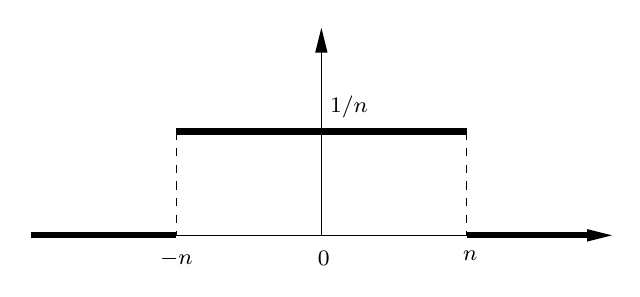
\begin{tikzpicture}[x=0.75pt,y=0.75pt,yscale=-1,xscale=1]
		%uncomment if require: \path (0,257); %set diagram left start at 0, and has height of 257

		\draw (80,170) -- (358,170) ;
		\draw [shift={(360,170)}, rotate = 180] [fill={rgb, 255:red, 0; green, 0; blue, 0 }  ][line width=0.08]  [draw opacity=0] (12,-3) -- (0,0) -- (12,3) -- cycle;
		\draw (220,170) -- (220,72) ;
		\draw [shift={(220,70)}, rotate = 90] [fill={rgb, 255:red, 0; green, 0; blue, 0 }  ][line width=0.08]  [draw opacity=0] (12,-3) -- (0,0) -- (12,3) -- cycle;
		\draw [line width=2.25](150,120) -- (290,120) ;
		\draw  [dashed, very thin]  (290,120) -- (290,170) ;
		\draw  [dashed, very thin]  (150,120) -- (150,170) ;
		\draw [line width=2.25](80,170) -- (150,170) ;
		\draw [line width=2.25](290,170) -- (350,170) ;

		\draw (287,176.4) node [anchor=north west][inner sep=0.75pt]  [font=\footnotesize]  {$n$};
		\draw (223,101.4) node [anchor=north west][inner sep=0.75pt]  [font=\footnotesize]  {$1/n$};
		\draw (141,176.4) node [anchor=north west][inner sep=0.75pt]  [font=\footnotesize]  {$-n$};
		\draw (217,176.4) node [anchor=north west][inner sep=0.75pt]  [font=\footnotesize]  {$0$};
		\end{tikzpicture}
		\caption{Plot of the function of example \vref{ex:strict-fatou}.}
	\end{figure}
	\FloatBarrier
	Then the $\liminf\limits_{n \to + \infty} f_n(t) = 0$ for all $t \in \RR$ but $\int_\RR f_n \de \lambda = 2 > 0 \quad \forall n \in \NN_0$.
\end{exam}


\begin{proof}
	Set $g_n(t) = \inf_{j\geq n}f_j(t)$. So $g_n$ is measurable and $g_{n+1}\geq g_n$ in $\Omega$.\\
	By definition of inferior limit we have:
	$$ \sup_{n\in \NN}g_n = \liminf_{n\to \infty} f_n.$$
	Using the monotone convergence theorem we get:
	$$\lim\limits_{n\to +\infty} \int_\Omega g_n\de \mu 
	= \int_\Omega \lim\limits_{n \to + \infty} g_n \de \mu 
	=\int_\Omega \liminf\limits_{n \to + \infty} f_n \de \mu$$
	By integral's monotonicity we obtain:
	$$\int_\Omega g_n \de\mu 
	\leq \int_\Omega f_n \de\mu;$$
	and considering the previous point we have:
	$$\lim\limits_{n \to + \infty}\int_\Omega g_n \de \mu \leq \liminf_{n \to + \infty} \int_\Omega f_n \de \mu$$
	which prove the thesis.
\end{proof}



%!TEX root = ../main.tex
\subsubsection{Derivative of a measure: definitions}\label{derivative-of-a-measure}

\paragraph{Measures defined through measurable functions} Here we see how a positive measurable function can provide an alternative measure.

\begin{theo}
	Let  $\phi: \Omega \to \left[0, +\infty\right]$ be a measurable function. Consider:
	$$\nu(E)\coloneqq\int_E \phi \,\de\mu \quad \text{for all } E \in \mm.$$
	Then, for any measurable function $f : \Omega \to \left[0, +\infty\right]$, $\nu(E)$ is a measure on $\mm$, and we have:
	$$\int_\Omega f \,\de\nu = \int_\Omega f \phi \,\de\mu.$$
\end{theo}

\begin{proof} \textit{Step 1, $\nu(E)$ is a measure on $\mm$}:\\
	It is easy to see that $\nu(\varnothing)=0 < +\infty$.\\
	Consider a sequence of mutually disjoint set $\{E_j\}_{j \in \NN} \subset\mm$ with $E=\bigcup_{j \in \NN}E_j$; using the monotone convergence for series (see corollary \vref{theo-beppo-series}), we have:
	\begin{align*}
		\nu(E) &= \int_E\phi \,\de\mu
		= \int_\Omega \phi \Ind_E \,\de\mu
		= \int_\Omega \sum_{j\in \NN}\phi \Ind_{E_j} \,\de\mu\\
		&= \sum_{j\in \NN} \int_\Omega \phi \Ind_{E_j} \,\de\mu
		= \sum_{j \in \NN} \int_{E_j} \phi \, \de \mu
		= \sum_{j\in \NN} \nu(E_j)
		;
	\end{align*}
	
	thus $\nu$ is countably additive.
	
	\textit{Step 2, exchange of measures}:\\
	Now let us focus on the second thesis of the theorem. It is enough to prove it when $f=\Ind_E$ with $E \in \mm$; then it can be easily extended to simple function and finally to positive functions by its approximation property. We have:
	$$
	\int_\Omega\Ind_E \,\de\nu 
	= \int_E d \nu 
	= \nu(E) 
	= \int_E \phi \,\de\mu 
	= \int_\Omega \phi \Ind_E \,\de\mu;$$
	that conclude the proof.
\end{proof}

In the first part of this proof we proved the following.
\begin{coro}
	Let $\phi$ be a positive and measurable function, and consider a sequence of disjoint sets $\{E_n\}_{n\in\NN}$. Then:
	$$\int_{\cup_{n \in \NN} E_n} \phi\, \de\mu = \sum_{n\in\NN}\int_{E_n} \phi \, \de\mu.$$
\end{coro}


\paragraph{Radon--Nikodym derivative} Suppose to have two measure, and we need to represent one in terms of the other. Possibly through an integral. This is possible by the followings.
\begin{defn}
	Consider a complete measure space $(\Omega,\mm,\mu)$ and a non-negative measurable function $\phi: \Omega \to [0,+\infty]$. If $\nu$ is such that:
	$$
		\nu(E) 
		= \int_E \phi \, \de \mu 
		\quad \text{for all }  E
	.
	$$
	Then $\phi$ is called \emph{Radon--Nikodym derivative} of $\nu$ with respect to $\mu$ and it is denoted by $\frac {\de\nu }{\de\mu}$.
\end{defn}
The integrand function is called ``derivative'' due to the analogy with the first fundamental theorem of calculus (see theorem \vref{theo-first-fundamental-calculus}) for which we have $F(x) = \int_a^x F'(t) \,\dt$.

For any measurable function $f:\Omega \to \left[0,+\infty\right]$ we can write:
\[
	\int_E f \,\de\nu =\int_E f \phi \,\de\mu = \int_E f \, \frac{\de\nu}{\de\mu} \,\de\mu
\]

Since we give the definition of Radon--Nikodym derivative, we ask ourselves if such function exists positive and measurable. We start observing that whenever the measure $\mu$ is zero on a set $E$, $\nu(E)$ must be zero too (otherwise we would have a null denominator and a non-null denominator). Indeed, if $\int_E f \,\de\nu = \int_E f \, \tfrac{\de\nu}{\de\mu} \,\de\mu$, then we require:
$$
	\mu(E) 
	= 0 
	\implies 
	\nu(E)
	= 0 
	\quad \text{for all } E \in \mm
.
$$
This motivates the following definition.

\begin{defn}
	We say that a measure $\nu$ is \emph{absolutely continuous} with respect to $\mu$, and we write $\nu \ll \mu$, if:
	$$
		\mu(E) 
		= 0 
		\implies \nu(E)
		= 0 
		\quad \text{for any } E \in \mm
	.
	$$
\end{defn}
In plain language, a measure $\nu$ is absolutely continuous with respect to $\mu$ if on all the sets for which $\mu$ is zero, $\nu$ is also zero.

This property holds when a measure can ``control'' the zero of another measure, it acquire a great meaning when considered with the previous definition: the measure $\mu$ controls the measure $\nu$ which was defined through $\mu$.

However, the condition $\nu \ll \mu$ is not sufficient alone for the existence of $\frac{\de\nu}{\de\mu}$; a sufficient condition for its existence in stated by the following theorem.

\begin{theo} [Radon--Nikodym] \label{theo-radon-nikodym}
	Let $(\Omega, \mm,\mu)$ be a complete measure space, and $\nu$, $\mu$ two measures on $(\Omega, \mm)$.\\
	If $\mu$ is $\sigma$-finite and $\nu\ll\mu$, then the Radon--Nikodym derivative $\frac{\de\nu}{\de\mu}$ exists.
\end{theo} 

See definition \vref{defn-positive-measure} for $\sigma$-finite. The theorem will be proved later on section \vref{proof-radon-nikodym}.

If $\mu$ is not $\sigma$-finite, then the existence of $\frac{\de\nu}{\de\mu}$ is not guaranteed.\\	
Indeed, consider the measure space $(\left[0,1\right],\Lc(\left[0,1\right]),\mu_c)$
where $\mu$ is the counting measure and let $\nu =\lambda\ll\mu_c$.
You can prove that there is no measure $\phi:\left[0,1\right] \to \left[0,+\infty\right]$ such that $\lambda(E) = \int_E \phi \, \de \mu_c \quad \forall E \in \Lc(\left[0,1]\right)$.
	
We will see that this is a powerful generalization of the second fundamental theorem of calculus (see theorem \vref{theo-2nd-found-calc}).
%\todo{Consider the following points}
%
%!!!! It is placed here (after fatou's lemma) because it is natural the possibility of define a measure from a measure using the integral
%
%!!!! It is an extension of the second fundamental theorem of calculus
%
%
%\begin{defn}
%	We say that $\mu$ is \emph{$\sigma$-finite} if there exists a sequence $\{E_j\}_{j \in \NN} \subset \mm$ such that:
%	$$\bigcup_{j\in\NN} E_j = \Omega \quad \text{and} \quad \mu(E_j) < +\infty \quad \forall j \in \NN$$
%\end{defn}
%
%\medskip
%\begin{exam}
%	\begin{enumerate}
%		\item The Lebesgue measure on $\RR^N$ is $\sigma$-finite;
%		\item the counting measure on $(\NN, \Pc(\NN)) $ is $\sigma$-finite;
%		\item the counting measure on $(\RR, \Lc(\RR)) $ is not $\sigma$-finite.
%	\end{enumerate}
%\end{exam}
%
%The following theorem states the sufficient conditions for the existence of $\frac{\de\nu}{\de\mu}$.


\newpage
\subsection{Lebesgue Integral}
%!TEX root = ../main.tex
Till now we worked only with positive valued functions, but they are not suitable for many application. The work of Henry Lebesgue (1875 - 1941) was not limited to those function, but it covered the case of a generic real valued function. Our aim now is to define the well-know integral named after him.

\subsubsection{Integrating real valued functions}

The first step is to establish what functions are integrable. Indeed, we already have a notion of Lebesgue integral, even it is limited to real valued functions we can use it to distinguish between functions. Any absolute value of a real valued function is a positive valued function; so the notion we already have can be used to define a space of integrable functions.

\begin{defn}\label{space-lebesgue-integrable-functions}
	Let $(\Omega, \mm, \mu)$ be a measurable space.\\
	We define the space of \emph{Lebesgue-integrable functions} as follows:
	$$
	\Lc_1(\Omega, \mm, \mu)
	\coloneqq \{f:\Omega \to \RR:\; f \text{ measurable and such that } \int_\Omega |f| \,\de\mu 
	< +\infty\}
	.
	$$
\end{defn}

Notice that need the hypothesis of measurability for this definition to have sense; take for instance the space $(\left[0,1\right],\Lc(\left[0,1\right]),\lambda)$, and consider the Vitali set $\Vc \subset [0, 1]$. Define $f$ as follows:
$$
	f(t) 
	\coloneqq \begin{cases}
		1 & \text{if }t \in \Vc \\
		-1 & \text{if }t \in \Vc\comp
	\end{cases}
.
$$
While $f$ is not measurable, $|f|$ is.

Here we can define an integral for real valued functions.

\begin{defn}
	Let $f \in \Lc^1 (\Omega, \mm, \mu)$. We define the \emph{Lebesgue abstract integral} of $f$ as follows:
	$$\int_\Omega f \de\mu \coloneqq \int_\Omega f^+ \de\mu - \int_\Omega f^- \de\mu$$
	where $f^+ = \max\{f,0\}$ and $f^- = -\min\{f,0\}$.\\
	In this case $f$ is called \emph{Lebesgue integrable function}.
\end{defn}

Notice that $0\leq f^+ \leq |f|$ and $0\leq f_- \leq |f|$ are both finite, thus also $\int_\Omega f \de\mu$ is finite, indeed we have just defined the Lebesgue \textit{abstract} integral.

For a complete discussion we present the following proposition. The notion of vector spaces will be discussed later (see definition \vref{defn-vector-spaces}).
\begin{prop}\label{prop-triang-ineq-integral}
	The set $\Lc^1(\Omega,\mm,\mu)$ is a vector space on $\RR$ with respect to the canonical operations $f+g$, $c \cdot f$ ($c \in \RR$).
	Indeed, the following inequalities holds:
	$$
		\left| \int_\Omega f \,\de\mu \right| 
		\leq \int_{\Omega} |f| \,\de\mu,
		\qquad \int_\Omega |f+g| \, \de \mu 
		\leq \int_\Omega|f| \, \de \mu + \int_\Omega |g| \, \de \mu
	.
	$$
\end{prop}
This last property, which is, in some sense, a generalization of triangular inequality, allow us to build an algebraic structure on this set.

Integrating on $\RR$'s intervals, the sign of the integral depends on its orientation. Here we define the actual standard.
\begin{defn}
	Consider $(\RR, \Lc(\RR), \lambda)$, for any interval $(a,b) \subset \RR$ we set this rule to change the orientation of the interval:
	$$\int_{a}^{b} f d \lambda \coloneqq \begin{cases}
	\int_{a}^{b} f d\lambda & \text{if } a < b \\
	0 & \text{if } a=b \\
	- \int_{b}^{a} f d\lambda & \text{if } a > b.
	\end{cases}$$
\end{defn}

Finally, a remark about series and the counting measure. Consider the measure space $(\NN, \Pc(\NN), \mu_c)$: the series $\{a_n\}_{n\in \NN}$ is Lebesgue integrable if and only if $\sum_{n \in \NN}|a_n| < +\infty$.
%!TEX root = ../main.tex
\subsubsection{Dominated convergence theorem} \label{dominated-convergence}
Having defined a general yet powerful notion of integral, our focus now is on building many tools that allow us to work on it. Some results are already been proved, the following result extend the monotone convergence (see \vref{monotone-convergence}) and the Fatou's lemma (see \vref{fatou-lemma}) to real valued functions.

\begin{theo}[Lebesgue's dominate convergence theorem]
	Let $(\Omega, \mm, \mu)$ measure space, $f_n : \Omega \to \RR$ measurable for all $n\in \NN$ such that:
	\begin{itemize}
		\item it point-wise converges $f_n(t) \to f(t)$ as $n \to +\infty$ for any $t \in \Omega$;
		\item exists a dominating function, namely $g:\Omega \to \RR$, which is Lebesgue-integrable and such that $|f_n(t)| \leq g(t)$ for all $t \in \Omega$ and for all $n \in \NN$.
	\end{itemize}
	Then $f_n, f\in \Lc^1(\Omega, \mm, \mu )$, and we have:
	$$\lim_{n\to \infty} \int_{\Omega} |f_n-f|\de\mu = 0$$
\end{theo}

Observe that the thesis implies the following:
$$\lim_{n \to +\infty} \int_\Omega \, f_n \de\mu = \int_{\Omega}\, f \de\mu;$$
indeed:
$$\left| \int_\Omega f_n \de\mu - \int_{\Omega} f \de\mu \right|
\leq \int_{\Omega}|f_n-f| \de\mu \to 0 \quad \text{as } n \to +\infty.$$
This shows how powerful and general is this theorem. In general the issue emerging when using it is to find a proper dominating function.

\begin{proof}
	Using the fact that $|f_n(t)| \leq g(t)$, it is easy to check from the definition that $f_n \in \Lc^1(\Omega, \mm , \mu)$ for any $n \in \NN$.\\
	In addiction, we know $f \in \Lc^1(\Omega, \mm , \mu)$, as $|f(t)| = \lim\limits_{n \to \infty}|f_n(t)|$ for all $n \in \NN$; this because: $$|\ |f(t)| -|f_n(t)|\ | \leq |f(t) - f_n(t)| \to 0.$$
	
	To prove the limit consider $\phi_n = 2g-|f_n-f|$.\\
	We have that $\phi_n$ are measurable, non-negative and converging: $\phi_n(t) \to 2g(t)$ for any $t \in \Omega$.\\
	Owing to Fatou's lemma we have:
	\begin{align*}
		0 \leq \int_{\Omega} 2 g \,\de\mu
		&=\int_{\Omega} \lim_{n \to +\infty} \phi_n \,\de\mu\\
		&\leq \liminf_{n \to +\infty} \int_{\Omega} \phi_n \,\de\mu\\
		&=\int_\Omega 2 g \,\de\mu
		+ \liminf_{n \to +\infty} \int_\Omega(-|f_n-f|) \,\de\mu.
	\end{align*}
	So we get:
	$$ 0 \leq \liminf_{n \to +\infty} \int_\Omega -|f_n-f| \,\de\mu$$
	which implies
	$$ \limsup_{n \to +\infty} \int_\Omega |f_n-f| \,\de\mu \leq 0$$
	and from this we can deduce the thesis:
	$$ \lim_{n \to +\infty} \int_\Omega |f_n-f| \,\de\mu = 0. $$
\end{proof}


\paragraph{Case of series of functions} The theorem can be formulated also for series of function as follows. To deeply understand this results remember that a series can be seen as the sequence of partial sum.

\begin{theo}[Dominate convergence theorem for series]
	Consider a sequence of functions $\{f_n\}_{n \in \NN} \subset \Lc^1(\Omega, \mm, \mu)$ for any $n \in \NN$ such that the series $\sum_{n \in \NN} f_n(t)$ converges point-wise $\forall t \in \Omega$, namely:
	$$\sum_{n\in \NN} \int_\Omega|f_n| \,\de\mu < +\infty.$$
	If exists a function $g \in \Lc^1(\Omega, \mm, \mu)$ such that:
	$$ \left|\sum_{j = 0}^n f_j(t)\right| 
	\leq g(t)
	\quad \forall n \in \NN
	\quad \forall t \in \Omega,$$
	then $\sum_{n\in\NN} f_n$ converges point-wise in $\Omega$ to a function $f\in \Lc^1(\Omega, \mm, \mu)$ and we have:
	$$\int_\Omega f \,\de\mu 
	= \int_\Omega \sum_{n \in \NN} f_n \, \de \mu 
	= \sum_{n\in \NN} \int_\Omega f_n \,\de\mu$$
\end{theo}



\begin{proof}
	Consider $\sum_{n\in \NN}|f_n|$ and observe that, by Beppo Levi's theorem:
	$$
		\int_\Omega \left(\sum_{n\in \NN} |f_n|\right) \,\de\mu 
		= \sum_{n\in \NN} \int_\Omega |f_n| \,\de\mu 
		< +\infty
	.
	$$
	Then $\sum_{n\in \NN} |f_n|$ converges a.e. in $\Omega$ to a $\tilde f \in \Lc^1(\Omega, \mm, \mu)$.
	Thus we also have that $\sum_{n\in \NN} f_n$ (absolutely) converges to some $f$ a.e. in $\Omega$, and moreover:
	$$
		\left| \sum_{n=0}^N f_n (t) \right|
		\leq \sum_{n=0}^N |f_n (t)|
		\leq \sum_{n=0}^{+\infty} |f_n (t)|
		= \tilde f(t)
	$$
	For almost any $ t \in \Omega$ and for all $N$.
	
	Thus we can apply dominated convergence to 
	$$
		F_N(t) 
		\coloneqq \sum_{n=0}^N f_n(t) \to f(t)
	.
	$$
	We have that $f\in \Lc^1(\Omega, \mm, \mu)$, and:
	$$
		\int_\Omega f \,\de\mu
		= \lim\limits_{N \to \infty} \int_\Omega F_N \,\de\mu
		= \lim\limits_{N \to \infty} \sum_{n=0}^N \int_\Omega f_n \,\de\mu
		= \sum_{n\in\NN} \int_\Omega f_n \,\de\mu
	.
	$$
\end{proof}
Notice that if $\int_\Omega \sum_{n \in \NN} |f_n| \,\de\mu < +\infty$ then $\sum_{n \in \NN} |f_n|$ is finite a.e. in $\Omega$ and $\sum f_n$ converges a.e. in $\Omega$.



%!TEX root = ../main.tex
\subsubsection{The almost everywhere concept}
By construction, Lebesgue integral is not conditioned by single points. In particular a countable set of points does not affect the result. At this point we have to ask ourself if this concept holds also for other properties. Suppose for example that a function satisfy a property except for a countable set of points, can we still apply the theorems that requires such property? The goal of this section is to extend all the previous results of abstract integration to functions defined up to a zero-measure set.

\begin{defn}
	A certain property $P(t)$, with $t\in \Omega$ holds \emph{almost everywhere (a.e.)} in $\Omega$ if:
	$$
		\mu(\{ \ 
			t\in \Omega: \neg P(t)
		\ \})
		=
		0
	.
	$$
\end{defn}

\begin{exam}
	The properties $P(t) = \{\sin(t) \neq 0\}$ and $Q(t) = \{\Ind_\QQ=0\}$\footnote{The function $\Ind_\QQ$, which is the indicator function on the rational number set, is called Dirichlet function.} hold a.e.\ in $\RR$.
	
\end{exam}


\paragraph{Extension of the measurability} The first property that we extend to this context from the general one is measurability:
\begin{defn}
	Let $(\Omega, \mm, \mu)$ be a complete measure space and $(X,\tau)$ a topological space.\\
	A function $f:(\Omega, \mm, \mu) \to (X,\tau)$ is \emph{measurable almost everywhere} in $\Omega$ if both
	$$\text{there exists } \Omega_0 \subset \Omega 
	\text{ such that } \mu(\Omega_0\comp)=0$$
	and
	$$f^{-1}(A) \cap \Omega_0 \in \mm 
	\text{ for all open set } A \subset X.$$
\end{defn}

This say that we require that the preimage of the function, intersected with a set $\Omega_0$ whose complement has zero measure, is still measurable: in this case the function is said to be measurable almost everywhere. In this way the function can be defined (or not) in $\Omega_0\comp$ in any manner without affecting its measurability.

It is easy to see that all the results proved so far, in particular Beppo Levi's, Fatou's and Lebesgue's, can be reformulated for functions defined almost everywhere and they still holds.

\paragraph{Essentially boundedness} In this context it is useful to give another definition of boundedness.
\begin{defn}
	A function $f:(\Omega, \mm, \mu) \to \RR$ is \emph{essentially bounded} if exists $M \geq 0$ such that:
	$$\mu (\{t \in \Omega: |f(t)|>M\})=0.$$
\end{defn}

The concept of almost everywhere allow us to redefine the supremum and the infimum of functions as well.
\begin{defn}
	Let $f:\Omega \to \RR$ be a measurable function.\\
	Then we define its \emph{essential supremum} in $\Omega$ as follows:
	$$\underset{t \in \Omega}{\esssup} f\coloneqq \inf \{M \geq 0 : \, \mu (\{t \in \Omega : |f(t)| > M\}) = 0\},$$
	and the \emph{essential infimum} in $\Omega$ as follows:
	$$\underset{t \in \Omega}{\essinf} f\coloneqq \sup \{M \geq 0 : \, \mu (\{t \in \Omega : |f(t)| < M\}) = 0\}.$$
\end{defn}

\begin{exam}
	Consider for example the Dirichlet function $f(t)=\Ind_\QQ(t)$ with $t \in \RR$. It is bounded and 
	$$
		\sup_\RR f 
		= \max_\RR f 
		= 1
	;
	$$ 
	it is essentially bounded as well, however: 
	$$
		\min \{M\geq 0; \, \lambda( t \in \RR : \Ind_\QQ (t) > 1 )\}
		= 0
	,
	$$
	which means 
	$$
		\esssup_\RR f 
		= \essinf_\RR f 
		= 0 
		\neq \sup_\RR f 
		= 1
	.
	$$ 
\end{exam}

\begin{exam}
	Consider now the following function:
	$$ 
		f(t) = \begin{cases}
			t e^{t^2} \quad & t \in \QQ \\
			\sin(t) \quad & t \in \QQ\comp
		;
		\end{cases}
	$$
	we have: 
	$$
		\esssup_\RR f = 1, 
		\quad \essinf_\RR f = -1, 
		\quad \sup_\RR f = + \infty, 
		\quad \inf_\RR f = - \infty
	.
	$$
\end{exam}


\paragraph{Extension of the continuity} Now we can discuss how also continuity can be defined almost everywhere:
\begin{defn}\label{def:continuity-almost-everywhere}
	Let $(\Omega, \Lc(\Omega),\lambda)$ be a complete measure space where $\Omega \subset \RR^N$ is an open set, and $(X,\tau)$ be a topological space.\\
	A function $f:(\Omega, \mm, \mu) \to (X,\tau)$ is \emph{continuous almost everywhere} in $\Omega$ if both
	$$
		\text{there exists } \Omega_0 
		\subset \Omega 
		\text{ such that } \mu(\Omega_0\comp)
		= 0
	$$
	and
	$$
		f^{-1}(A) \cap \Omega_0 
		\text{  is open for all open set } A 
		\subset X
	.
	$$
\end{defn}
Equivalently a function is continuous a.e.\ if the measure of its discontinuity points is zero.

Observe that if a function is continuous a.e.\ then it's Lebesgue measurable a.e..

\begin{prop}
	Consider two continuous functions $f,g: \RR \to \RR$.\\
	If they coincide a.e.\,
	namely
	$$
		f
		=g 
		\ a.e.
		\text{ with respect to } \lambda
	,
	$$
	then they coincide at any point,
	namely:
	$$
		f(t)
		= g(t) 
		\text{ for any } 
		t \in \RR
	.
	$$
\end{prop}
\begin{proof}
	By contradiction, if there exists $x_0 \in \RR$ such that $f(x_0)\neq g(x_0)$
	then by continuity there exists also a $\delta$ such that
	$f(x) \neq g(x)$
	for all $x \in (x_0 - \delta, x_0 + \delta)$.\\
	But then $\lambda((x_0-\delta,x_0+\delta))=2\delta>0$:
	so there exists an interval of positive measure where the two functions are different, so we have a contradiction.
\end{proof}

\begin{exam}
	Consider again the Dirichlet function $f(t)=\Ind_\QQ(t)$; it is nowhere continuous (it is not continuous a.e. in $\RR$).\\
	However $f = 0 \ a.e.$, so $f$ is equal a.e. to a continuous function. This while the Heaviside function $H = \Ind_{[0,+\infty)}$ is continuous a.e. but it is not equal a.e. to any continuous function. You can prove this. The same consideration can be done for the following: 
	$$
		f(x) 
		\coloneqq \begin{cases}
			\frac x{|x|} & x \neq 0 \\ 0 & x=0
			\end{cases}
	.
	$$
\end{exam}

\begin{exam}
	Consider also the function we seen right before: 
	$$ 
		f(t) = \begin{cases}
		t e^{t^2} 
		\quad & t \in \QQ \\
		\sin(t) \quad & t \in \QQ\comp
		;
		\end{cases}
	$$
	we see that it is not bounded but it is essentially bounded. It is continuous in $t=0$; think whether it is continuous elsewhere!
\end{exam}

\begin{exam}
	At last consider the function $f: \RR \to \RR^\star$ defined in this way:
	$$
		f(t) 
		\coloneqq \begin{cases}
			\arctan(t) & t \in \QQ\comp\\
			+\infty & t \in \QQ \cup [0,+\infty)\\
			-\infty & t \in \QQ \cup (-\infty,0]
			;
		\end{cases}
	$$
	this function is equal a.e. to a continuous function but it's nowhere continuous, it isn't bounded while is essentially bounded.\\
	Same result with 
	$$
		f(t) 
		\coloneqq \begin{cases} 
			\sin(t) & f \in \RR \setminus \QQ \\
			-\infty & t \in \QQ_- \\ 
			+\infty & t \in \QQ_+
			.
		\end{cases}
	$$
\end{exam}

\begin{prop}
	Consider a function $f: (\Omega, \Lc(\Omega),\lambda) \to \RR$, with $\Omega \subset \RR^N$.\\
	As $f$ is Lebesgue measurable, there exists a function $g:\Omega\to \RR$ which is Borel measurable and such that $f = g$ a.e.\ in $\Omega$.
\end{prop}

\paragraph{Extension of convergence theorems} The three convergence theorems, which are the Beppo Levi's or monotone convergence theorem (see theorem \vref{monotone-convergence}), the Fatou's lemma (\vref{fatou-lemma}) and the dominated convergence theorem (\vref{dominated-convergence}), can be trivially reformulated for measurable a.e.\ functions.

In addiction we can prove another theorem for convergence of series of function:

\begin{theo}
	Consider a sequence of functions $\{f_n\}_{n \in \NN} \subset \Lc^1(\Omega, \mm, \mu) \ \forall n \in N$ such that the series $\sum_{n \in \NN} f_n(t)$ converges point-wise $\forall t \in \Omega$, namely:
	$$\sum_{n\in \NN} \int_\Omega|f_n| \,\de\mu < +\infty.$$
	Then $\sum_{n\in\NN} f_n$ converges a.e in $\Omega$ to a function $f\in \Lc^1(\Omega, \mm, \mu)$ and we have:
	$$\int_\Omega f \,\de\mu 
	= \int_\Omega \sum_{n \in \NN} f_n \, \de \mu 
	= \sum_{n\in \NN} \int_\Omega f_n \,\de\mu.$$
\end{theo}
\begin{proof}
	The series $\sum_{n\in \NN}|f_n|$ converges to a non-negative function $g$ and, by Beppo Levi's theorem:
	$$ \int_\Omega \left(\sum_{n\in \NN} |f_n|\right) \,\de\mu = \sum_{n\in \NN} \int_\Omega |f_n| \,\de\mu < +\infty.$$
	Then we say that $\sum_{n\in \NN} |f_n|$ converges a.e. in $\Omega$ to $g \in \Lc^1(\Omega, \mm, \mu)$;	we have that $\sum_{n\in \NN} f_n$ absolutely converges to some $f$ a.e. in $\Omega$, and moreover:
	$$
		\left| \sum_{n=0}^N f_n (t) \right|
		\leq \sum_{n=0}^N |f_n (t)|
		\leq \sum_{n=0}^{+\infty} |f_n (t)|
		= g(t)
	$$
	for almost any $t \in \Omega$ and for all $N$.
	
	Thus we can apply dominated convergence to $\sum_{n=0}^N f_n(t) \to f(t)$. \\
	We have that $f\in \Lc^1(\Omega, \mm, \mu)$, and:
	$$
		\int_\Omega f \,\de\mu
		= \lim\limits_{N \to \infty} \int_\Omega \sum_{n=0}^N f_n(t) \,\de\mu
		= \lim\limits_{N \to \infty} \sum_{n=0}^N \int_\Omega f_n \,\de\mu
		= \sum_{n\in\NN} \int_\Omega f_n \,\de\mu
	.
	$$
\end{proof}
Notice that if $\int_\Omega \sum_{n \in \NN} |f_n| \,\de\mu < +\infty$ then $\sum_{n \in \NN} |f_n|$ is finite a.e. in $\Omega$ and $\sum f_n$ converges a.e. in $\Omega$.

\paragraph{Further results} Here we introduce some other results that can be proven at this state of the theory. First we talk about a useful inequality widely used in probability.
\begin{prop}[Chebyshev's inequality]
	Let $f \in \Lc^1(\Omega, \mm, \mu)$ such that $f \geq 0$ a.e. in $\Omega$, $c>0$.\\
	Then the following inequality holds: 
	$$
		\mu(\{t \in \Omega : f(t) \geq c\})
		\leq \frac 1 c \int_\Omega f \,\de\mu
	.
	$$
\end{prop}
This inequality is trivial if we think to its geometrical meaning.
\begin{figure}[htpb]
	\centering
	\tikzset{every picture/.style={line width=0.75pt}} %set default line width to 0.75pt        

	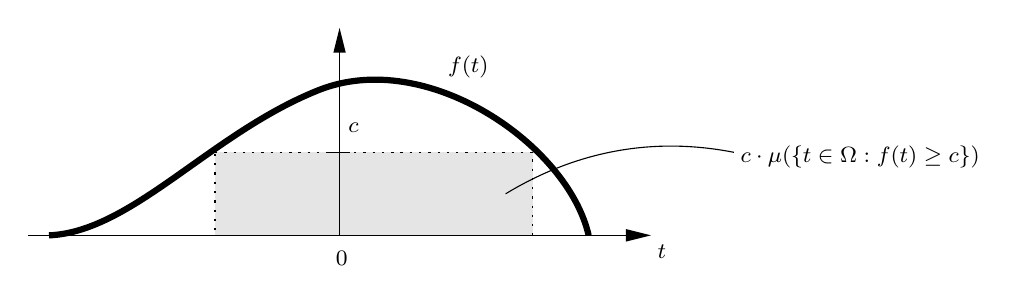
\begin{tikzpicture}[x=0.75pt,y=0.75pt,yscale=-1,xscale=1]
	%uncomment if require: \path (0,257); %set diagram left start at 0, and has height of 257

	\draw (70,170) -- (368,170);
	\draw [shift={(370,170)}, rotate = 180] [fill={rgb, 255:red, 0; green, 0; blue, 0 }  ][line width=0.08]  [draw opacity=0] (12,-3) -- (0,0) -- (12,3) -- cycle;
	\draw (220,170) -- (220,72);
	\draw [shift={(220,70)}, rotate = 90] [fill={rgb, 255:red, 0; green, 0; blue, 0 }  ][line width=0.08]  [draw opacity=0] (12,-3) -- (0,0) -- (12,3) -- cycle;
	\draw [line width=2.25] (80,170) .. controls (120,168.36) and (158,120.64) .. (210,100) .. controls (262,79.36) and (330,126.36) .. (340,170);
	\draw  [fill={rgb, 255:red, 0; green, 0; blue, 0 }  ,fill opacity=0.1 ][dash pattern={on 0.84pt off 2.51pt}] (160,130) -- (313,130) -- (313,170) -- (160,170) -- cycle;
	\draw (300,150) .. controls (334,129.36) and (371,122.36) .. (410,130);
	\draw (225,130) -- (215,130);

	\draw (217,176.4) node [anchor=north west][inner sep=0.75pt]  [font=\footnotesize]  {$0$};
	\draw (271,82.4) node [anchor=north west][inner sep=0.75pt]  [font=\footnotesize]  {$f(t)$};
	\draw (223,114.4) node [anchor=north west][inner sep=0.75pt]  [font=\footnotesize]  {$c$};
	\draw (412,125.4) node [anchor=north west][inner sep=0.75pt]  [font=\footnotesize]  {$c\cdot \mu ( \{t\in \Omega:f( t) \geq c\})$};
	\draw (372,173.4) node [anchor=north west][inner sep=0.75pt]  [font=\footnotesize]  {$t$};
	\end{tikzpicture}
\end{figure}
\FloatBarrier
\begin{proof}
	Consider the following chain of inequalities:
	$$
		\int_\Omega f \, \dmu 
		\geq \int_{\{t \in \Omega : \, f(t) \geq c\}} f \, \dmu
		\geq c \cdot \mu(\{t \in \Omega: \, f(t) \geq c\})
	.
	$$
\end{proof}

Here another useful tool:
\begin{prop} \label{integral-inequality-sigma-finite}
	Let $(\Omega, \mm, \mu)$ be a $\sigma$-finite measure space.\\
	Consider two measurable functions $f,g: \Omega \to [0, +\infty]$ such that:
	$$
		\int_E f \, \de \mu \leq
		\int_E g \, \de \mu
		\quad \text{for all } E \in \mm
	,
	$$
	then $f\leq g$ almost everywhere in $\Omega$.
\end{prop}

Lastly we present a simple yet useful result:
\begin{theo}[Vanishing lemma]\label{vanishing-lemma}
	Let $f\in \Lc^1(\Omega, \mm, \mu)$ such that $f\geq 0$ a.e. in $\Omega$.
	$$
		\text{If }\int_\Omega f \,\de\mu = 0\text{ then }f = 0 \text{ a.e. in } \Omega.$$
\end{theo}
\begin{proof}
	Take the following set for each $n \in\NN_0$:
	$$
		E_n 
		= \{t \in \Omega : f(t) \geq \frac 1 n \} \in \mm
	.
	$$
	Then:
	$$ 
		0 
		= \int_\Omega f \,\de\mu 
		\geq \int_{E_n} f \,\de\mu 
		\geq \frac 1 n \mu (E_n)
		\quad \forall n \in \NN_0
	.
	$$
	Thus $\mu(E_n) = 0$ for all $n \in \NN_0$.
	
	Now suppose there exists $t \in \Omega$  such that $f(t) > 0$.\\
	Then it exists $n_0 \in \NN$ such that $f(t) \geq \frac 1 {n_0}$, and so
	$$t \in E_{n_0}\subset E \text{ where } E = \bigcup_{n\in \NN_0} E_n.$$\\
	Thus $\{t\in \Omega : f(t) > 0\} \subseteq E$, so: 
	$$\mu (E) \le \sum_{n \in \NN} \mu(E_n) = 0.$$
\end{proof}


A brief final remark: consider $\Lc^1(\Omega, \mm, \mu)$ and define $d(f,g) \coloneqq \int_\Omega |f,g| \,\de\mu$. Notice that such function is not a metric: indeed, by the vanishing lemma, $d(f,g)=0 \implies f=g$ not everywhere, but \textit{almost} everywhere $\in \Omega$.\\
To solve the problem, we consider the following equivalence relation: $$f \sim g \iff f=g \text{ a.e. in } \Omega$$
Take the quotient set $X_1 \coloneqq \frac{\Lc^1(\Omega, \mm, \mu)}{\sim}$. Then $d$ is a metric in $X_1$.

%
%
%
%
%\subsection{Comparison between Lebesgue and Riemann integral}
%
%In this section we will consider the space $(\RR, \Lc(\RR), \lambda)$, and we will focus on intervals.
%
%\begin{theo}
%	Let $a,b \in \RR: a<b$, $f:(a,b) \to \RR$ bounded. \\
%	Then $f$ is \emph{Riemann-integrable} in $(a,b)$ if and only if $f$ is continuous a.e. in $(a,b)$.
%\end{theo}
%
%Notice that $\Ind_{\QQ \cap (a,b)}$ is not Riemann integrable, because it is nowhere continuous. But $\Ind_{\QQ \cap (a,b)}=0$ a.e. in $(a,b)$, it is Lebesgue-integrable, and $\int_a^b \Ind_{\QQ \cap (a,b)} \dlam =0$.
%
%More in general, if $f: (a,b) \to \RR$ is Lebesgue-measurable and bounded, then $f$ is Lebesgue integrable.
%
%\begin{theo}
%	Let $f:(a,b)\subset \RR \to \RR$ be bounded and continuous a.e. in $(a,b)$. Then:$$ \underbrace{\int_a^b f(t) \,\dt}_{Riemann}
%	= \underbrace{\int_a^b f(t) \,\dlam}_{Lebesgue}$$
%\end{theo}
%
%For the proof see k-f pp 309-310.
%
%Let us now focus on improper Riemann integrals, where $f$ and/or the integration domain is unbounded. We have: %rewrite
%\begin{theo}
%	Let $f: (a,b) \subseteq \RR \to \RR$, with $a,b\in \RR^\star : a< b$.
%	
%	If $f$ is Riemann integrable in $(a,b)$ in the improper sense and it changes its sign at most a finite number of times, then	$f$ is Lebesgue integrable in $(a,b)$ and the two integrals coincide.
%\end{theo}
%
%\begin{proof}
%	Suppose $f>0$. We can find two sequences, $\{a_n\}_{n\in \NN}$ and $\{b_n\}_{n\in \NN}$, such that $a_n < b_n$, $a_n \downarrow a$, $b_n \uparrow b$, and $(a,b)=\bigcup_{n\in \NN} (a_n,b_n)$.
%	
%	Suppose $f$ is bounded on $(a_n,b_n) \ \forall n \in \NN$.\\
%	Therefore $f$ is Riemann integrable on each $(a_n,b_n)$ and we have:
%	\begin{align*}
%	\underbrace{\int_{a_n}^{b_n} f(t) \,\dt}_{Riemann}
%	&= \underbrace{\int_{a_n}^{b_n} f(t) \,\dlam}_{Lebesgue}
%	\quad \forall n \in \NN
%	\intertext{Set $F_n \coloneqq \bigcup_{j=0}^n (a_j,b_j)$ and $f_n \coloneqq f \Ind_{F_n}$. $f_n \uparrow f$ and, using Beppo Levi's theorem, we have:}
%	\int_a^b f(t) \,\dlam
%	&= \lim_{n \to \infty} \int_a^b f_n(t) \,\dlam
%	= \lim_{n \to \infty} \int_{a_n}^{b_n} f(t) \,\dlam
%	\intertext{By definition of Riemann improper integral, we have:}
%	\int_a^b f(t) \,\dt
%	&= \lim_{n \to \infty} \int_{a_n}^{b_n} f(t) \,\dt
%	\end{align*}
%	Putting all together, we get the thesis.
%\end{proof}
%
%Notice that there functions which are Riemann- but not Lebesgue-integrable.
%\begin{exam}
%	$$f(t)=\frac {\sin t}{t} \quad t \in (0,+\infty)$$
%	$f$ is Riemann-integrable: $\lim\limits_{a \to +\infty} \int_0^a f(t) \,\dt$ exists. However:\todo{Explain better?}
%	$$ \int_0^{+\infty} \left| \frac{ \sin t}{t} \right| \dlam
%	= \int_0^{+\infty}\frac 1 t \dlam = +\infty $$
%	Thus $f$ is not Lebesgue-integrable.
%\end{exam}
%
%%reload
%\medskip
%\begin{exam}
%	Consider the following function:
%	$$f(t)\coloneqq\begin{cases}
%	\sin(t) & \text{if } t \in \RR \setminus \ZZ \\ 
%	+ \infty & \text{if } t \in \ZZ^+ \\ 
%	- \infty & \text{if } t \in \ZZ_-	
%	\end{cases} $$
%	
%	$f$ is essentially bounded and continuous a.e. in $\RR$, and $f(t) = \sin(t)$ a.e. in $\RR$.
%\end{exam}
%
%\medskip
%\begin{exam}
%	Consider the following function:
%	$$f(t)\coloneqq\begin{cases} 
%	\sin(t) 		& \text{if } t \in \left[0,1\right]\cap \left(\RR \setminus \QQ \right) \\
%	+ \infty 	   &  \text{if } t \in \left[0,1\right]\cap \QQ
%	\end{cases}$$
%	
%	$f$ is nowhere continuous, bounded, and measurable. Then that $f$ is Lebesgue integrable, hence $\int_0^1 f(t) \,\dlam$ exists finite.
%	
%	Indeed, $f(t) = \sin (t)$ $a.e.$ in $\left[0,1\right]$, thus:
%	$$\int_0^1 f(t) d \lambda =\underbrace{\int_0^1 \sin t \,\dlam}_{Lebesgue}
%	=\underbrace{\int_0^1 \sin t \,\dt}_{Riemann}$$
%\end{exam}
%
%Notice that there are some functions which are $\Lc$-integrable but they are not even equal a.e. to a R-integrable function. For instance, consider the characteristic function of a generalized Cantor set.

%!TEX root = ../main.tex
\subsubsection{Derivative of a measure: properties}
Now we are ready to proceed in theory development about derivatives. With the definition of almost everywhere we can talk about uniqueness and some properties.

\begin{prop}
	If the hypothesis of the Radon--Nikodym theorem (\vref{theo-radon-nikodym}) hold, then the Radon--Nikodym derivative is unique almost everywhere.
\end{prop}
The reader can easily prove this result using proposition \vref{integral-inequality-sigma-finite}. Do it now before see the following proof!

\begin{proof}
	Consider two Radon--Nikodym derivatives for $\frac{\dnu}{\dmu}$: two positive and measurable function $\phi_1$ and $\phi_2$.\\
	Then we have: $$\int_E \phi_1 \dmu = \int_E \phi_2 \dmu \quad \text{for all } E \in \mm.$$
	From the previously referenced proposition we have both $\phi_1 \geq \phi_2$ and $\phi_2 \geq \phi_1$ a.e.\ in $\Omega$, hence the thesis.
\end{proof}

Moreover, it holds the following.
\begin{prop}
	If the Radon--Nikodym derivative $\phi$ exists and $\mu (\Omega) < +\infty$, then $\phi \in L^1(\Omega, \mm, \mu)$. 
\end{prop}
%
%\begin{rema}
%	$f:\Omega \to \RR$ is measurable. Then:
%	$$f \in L^1(\Omega, \mm, \nu) \iff f \frac{\de\nu}{\de\mu} \in L^1(\Omega, \mm, \mu)$$
%\end{rema}
%The proof of this result is also left as an exercise for the reader.

\paragraph{Basic properties} Here we present some properties of the Radon--Nikodym derivative.

\begin{prop}[Change of measure]
	For any measurable positive function $f:\Omega \to [0,\infty]$ we have:
	$$ \int_\Omega f \, \de \nu = \int_\Omega f \, \frac{\de \nu}{\de \mu} \de \mu.$$
\end{prop}

\begin{prop}[Linearity of the derivative]
	For all $c_1, c_2 \geq 0$ we have:
	$$\dfrac{\de(c_1\nu_1+c_2\nu_2)}{\de\nu} = c_1 \dfrac{\de\nu_1}{\de\mu}+ c_2 \dfrac{\de\nu_2}{\de\mu}.$$
\end{prop}

\begin{prop}[Chain rule]
	Consider three measures $\lambda$, $\nu$ and $\mu$ such that $\lambda \ll \nu \ll \mu$.\\
	Then we have:
	$$\dfrac{\dlam}{\de\mu} =
	\dfrac {\de \lambda}{\de\nu} \dfrac{\de\nu}{\de\mu}.$$
\end{prop}
\begin{proof}
	For every $E \in \mm$ observe that:
	$$
		\lambda(E)
		= \int_E\frac{\dlam}{\de\nu} \,\de\nu
		= \int_E \frac{\dlam}{\de\nu}\frac{\de\nu}{\de\mu} \,\dmu
	;
	$$
	moreover, as $\lambda \ll \mu$, we have that:
	$$
		\lambda(E)
		= \int_E \frac{\dlam}{\de\mu} \de\mu
	,
	$$
	and then, on account of \vref{integral-inequality-sigma-finite}:
	$$
		\frac{\dlam}{\de\mu}
		= \frac{\dlam}{\de\nu}\frac{\de\nu}{\de\mu}
		\quad \text{a.e.}
	.
	$$
\end{proof}

\begin{prop}[Inverse derivative]
	If $\nu \ll \mu$ and $\mu \ll \nu$ then we have:
	$$\dfrac {\de\nu}{\de\mu} =
	\left(\dfrac{\de\mu}{\de\nu}\right)^{-1}.$$
\end{prop}
\begin{proof}
	For every $E \in \mm$ we have that:
	$$\mu(E) =\int_E \de\mu 
	= \int_E \frac{\de\mu}{\de\nu}\de\nu
	= \int_E \frac{\de\mu}{\de\nu}\frac{\de\nu}{\de\mu}\de\mu$$
	thus, always on account of \vref{integral-inequality-sigma-finite}:
	$$1 =
	\frac{\de\mu}{\de\nu}\frac{\de\nu}{\de\mu}
	\quad \text{a.e.}.$$
\end{proof}
%!TEX root = ../main.tex
\subsubsection{Metric spaces and convergences}

In this part we will see how the tools we developed can be deployed in practice. First we extend the notion of Lebesgue integrability by using the concept of almost everywhere. The we see how handle different kind of limits of series of functions.

\paragraph{The space $L^1$} As we discovered that many properties can be useful even when they holds almost everywhere, now we can find a space wider than $\Lc_1$ but whose functions has the same properties.

\begin{defn}\label{L1-space}
	Consider the space $\Lc_1(\Omega, \mm, \mu)$ and define on it the following equivalence relation: 
	$$
		f \sim g 
		\quad \text{ if }  
		f = g 
		\text{ a.e. in }\Omega
	;
	$$
	we define the \emph{space $L_1$} by the quotient set:
	$$L_1(\Omega, \mm, \mu)=\frac{\Lc_1(\Omega, \mm, \mu)}{\sim}.$$
\end{defn}

In plain language, this set contains all the functions which are equal almost everywhere to a function in $\Lc^1$.
For the definition of quotient set see \vref{defn-equiv-class-quot-set}.

Such set is a vector space on $\RR$ with respect to the canonical operations sum $[f]+[g]=[f+g]$ and homogeneity $[c f] = c[f]$, $c \in \RR$.\\
It is also a metric space with respect to the following distance:
$$
	d_1 
	\coloneqq \int_\Omega |f-g| \, \de \mu
	\text{ for all } [f],[g]
	\in L_1(\Omega, \mm, \mu)
,
$$
and is proved that $L^1$ with $d_1$ is a complete metric space.\\
However, $\Lc_1$ isn't a metric space with respect to the distance $d_1$ as $d_1(f,g) = 0$ implies only that $f=g$ a.e. in $\Omega$.

As $L^1$ is a metric space we can develop a proper notion of convergence on it.

\paragraph{Convergence of series of functions} There are four notions of convergence in a measure space: we will introduce the definition and we analyze the relations between them.
\begin{defn}
	Let $(\Omega, \mm, \mu)$ be a complete measure space, and $\{f_n\}_{n\in \NN}$ be a sequence of measurable functions such that $f_n : \Omega \to \RR$:
	\begin{itemize}
		\item we say that $f_n(t)$ \emph{converges point-wise almost everywhere} to $f(t)$ as $n\to \infty$,
			and we write ``$f(t)_n \aeto f(t)$'',
			if we have:
			$$
				\mu (\{t \in \Omega: \lim\limits_{n \to +\infty} f_n(t) \neq f(t)\})
				= 0
			;
			$$
			
		\item we say that $f_n(t)$ \emph{converges uniformly almost everywhere} to $f(t)$ as $n\to \infty$,
			and we write ``$f(t)_n \uaeto f(t)$'',
			if we have:
			$$
				\lim\limits_{n \to +\infty}\underset{\Omega}{\esssup} |f_n-f| 
				= 0
			;
			$$
			
		\item we say that $f_n(t)$ \emph{converges in mean} to $f(t)$ as $n\to \infty$,
			and we write ``$f(t)_n \lto{1} f(t)$'',
			if $\{f_n\}_{n \in\NN} \subset L^1(\Omega, \mm, \mu)$ and: 
			$$
				\lim\limits_{n \to +\infty} \int_\Omega |f_n-f| \,\de \mu 
				= 0
			;
			$$
			
		\item we say that $f_n(t)$ \emph{converges in measure} to $f(t)$ as $n\to \infty$,
			and we write ``$f(t)_n \mto f(t)$'',
			if we have:
			$$
				\forall \varepsilon >0 
				\quad \lim\limits_{n \to +\infty} \mu(\{t\in \Omega : |f_n (t)-f(t)| > \varepsilon \}) 
				= 0
			.
			$$
	\end{itemize}
\end{defn}
To memorize those definition notice that there are some elements that are common; the following observations can help to understand and memorize:
\begin{itemize}
	\item the $\lim_{n \to \infty}$ occurs in all definitions;
	\item all definitions states that some quantity is equal to zero;
	\item all definitions involves the set $\Omega$;
	\item all definitions involves the measure $\mu$, the first and the second through a measure of a set, the third through the integral, and the second through the $\esssup$, which is defined in accordance to a measure.
	\item all definitions involves $f_n - f$, which, in different ways, tends to zero. Also the first contains this subtraction implicitly;
	\item notice that the third definition requires also that the functions are integrable a.e.;
	\item the first definition consist of a measure of the set in which a limit does not occur, viceversa the third is the limit of the measure of a set.
\end{itemize}

It's clear that this definitions are not fully equivalent each other, but they are somehow correlated. Here we try to investigate their relations by declaring and proving some propositions.

Some observation before starting the comparisons. Notice that the main vantage of uniform convergence over point-wise is that with uniform convergence we have not any dependence form the points of the domain $t$.\\ 
Notice that the integral in the mean convergence contains the distance $d_1$ (the module): that is a metric convergence.\\
The convergence in measure is widely used in probability.

\paragraph{Uniform a.e.\ convergence implies point-wise a.e.\ convergence} This result is stated in the following proposition:
\begin{prop}\label{convergence-uniform-implies-point-wise}
	If a series of function converges uniformly almost everywhere, then such series also converges point-wise almost everywhere.
\end{prop}
The proof is very easy. Do it!\\

\paragraph{Point-wise a.e.\ convergence does NOT imply uniform a.e.\ convergence} Consider the following series of functions:
$$f_n(t) = \begin{cases}
nt & \text{if }0 \leq t \leq \frac 1 n \\
2-nt & \text{if }\frac 1 n \leq t \leq \frac 2 n \\
0 & \text{if }\frac 2 n \leq t \leq 1
\end{cases}$$

\begin{figure}[htpb]
	\centering
	\tikzset{every picture/.style={line width=0.75pt}} %set default line width to 0.75pt        

	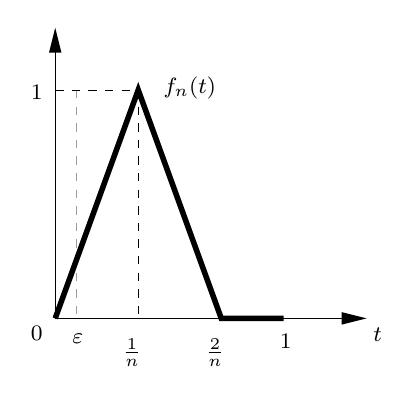
\begin{tikzpicture}[x=0.75pt,y=0.75pt,yscale=-1,xscale=1]
	%uncomment if require: \path (0,257); %set diagram left start at 0, and has height of 257

	\draw [color={rgb, 255:red, 155; green, 155; blue, 155 }  ,draw opacity=1 ] [dashed, very thin]  (230,60) -- (230,170);
	\draw (220,170) -- (368,170);
	\draw [shift={(370,170)}, rotate = 180] [fill={rgb, 255:red, 0; green, 0; blue, 0 }  ][line width=0.08]  [draw opacity=0] (12,-3) -- (0,0) -- (12,3) -- cycle;
	\draw (220,170) -- (220,32);
	\draw [shift={(220,30)}, rotate = 90] [fill={rgb, 255:red, 0; green, 0; blue, 0 }  ][line width=0.08]  [draw opacity=0] (12,-3) -- (0,0) -- (12,3) -- cycle;
	\draw [line width=2] (220,170) -- (260,60) -- (300,170) -- (330,170);
	\draw  [dashed, very thin]  (260,60) -- (260,170);
	\draw  [dashed, very thin]  (220,60) -- (260,60);

	\draw (207,172.4) node [anchor=north west][inner sep=0.75pt]  [font=\footnotesize]  {$0$};
	\draw (251,178.4) node [anchor=north west][inner sep=0.75pt]  [font=\footnotesize]  {$\frac{1}{n}$};
	\draw (327,176.4) node [anchor=north west][inner sep=0.75pt]  [font=\footnotesize]  {$1$};
	\draw (372,173.4) node [anchor=north west][inner sep=0.75pt]  [font=\footnotesize]  {$t$};
	\draw (291,178.4) node [anchor=north west][inner sep=0.75pt]  [font=\footnotesize]  {$\frac{2}{n}$};
	\draw (207,56.4) node [anchor=north west][inner sep=0.75pt]  [font=\footnotesize]  {$1$};
	\draw (271,52.4) node [anchor=north west][inner sep=0.75pt]  [font=\footnotesize]  {$f_n(t)$};
	\draw (227,176.4) node [anchor=north west][inner sep=0.75pt]  [font=\footnotesize]  {$\varepsilon $};
	\end{tikzpicture}
\end{figure}
\FloatBarrier

In this case $f_n(t) \to 0$ for all $t \in \left[0, 1\right]$, and thus $f_n \aeto 0$.\\
However, $\esssup|f_n| = 1$ and so it does not converge to $0$, so $f_n \xslashedrightarrow{\text{u.a.e.}} f=0$.

Notice that to obtain also uniformly convergence we should consider the interval $[\eps, 1]$, with $\eps > 0$.\\
In general this little trick hols, indeed we have:

\begin{prop}[Severini--Egorov]\label{prop-sever-egoro}
	If $\mu(\Omega) < +\infty$ and $f_n \aeto f$, then\footnote{For further discussion, see: R. L. Wheeden, A. Zygmund, Measure and Integral: An Introduction to Real Analysis (2015), page 245, theorem 10.14.}
	$$\text{for all } \varepsilon > 0 \text{ there exists } E \subset \mm$$
	such that 
	$$\mu(E\comp)<\eps \text{ and } f_n \uaeto f \text{ in } E.$$
\end{prop}

This theorem provide us a condition for which point-wise a.e. convergence implies uniform a.e. convergence, restoring the inverse implication.

If $\mu(\Omega)=+\infty$, the theorem might not hold, as shown in the following counterexample. On $(\RR,\Lc(\RR),\lambda)$ take:
	$$f_n(t) = \begin{cases}
	1 & \text{if } t\in\left[n,n+1\right]\\
	0 & \text{elsewhere} .
	\end{cases}$$
\begin{figure}[htpb]
	\centering
	\tikzset{every picture/.style={line width=0.75pt}} %set default line width to 0.75pt        

	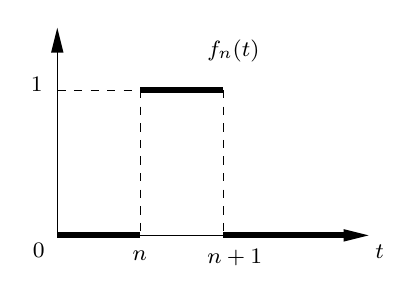
\begin{tikzpicture}[x=0.75pt,y=0.75pt,yscale=-1,xscale=1]
	%uncomment if require: \path (0,257); %set diagram left start at 0, and has height of 257

	\draw    (220,170) -- (368,170) ;
	\draw [shift={(370,170)}, rotate = 180] [fill={rgb, 255:red, 0; green, 0; blue, 0 }  ][line width=0.08]  [draw opacity=0] (12,-3) -- (0,0) -- (12,3) -- cycle    ;
	\draw    (220,170) -- (220,72) ;
	\draw [shift={(220,70)}, rotate = 90] [fill={rgb, 255:red, 0; green, 0; blue, 0 }  ][line width=0.08]  [draw opacity=0] (12,-3) -- (0,0) -- (12,3) -- cycle    ;
	\draw  [dashed, very thin]  (260,100) -- (260,170) ;
	\draw [line width=2.25]    (260,100) -- (300,100) ;
	\draw  [dashed, very thin]  (300,100) -- (300,170) ;
	\draw [line width=2.25]    (220,170) -- (260,170) ;
	\draw [line width=2.25]    (300,170) -- (360,170) ;
	\draw  [dashed, very thin]  (220,100) -- (260,100) ;

	\draw (207,172.4) node [anchor=north west][inner sep=0.75pt]  [font=\footnotesize]  {$0$};
	\draw (372,173.4) node [anchor=north west][inner sep=0.75pt]  [font=\footnotesize]  {$t$};
	\draw (206,92.4) node [anchor=north west][inner sep=0.75pt]  [font=\footnotesize]  {$1$};
	\draw (291,74.4) node [anchor=north west][inner sep=0.75pt]  [font=\footnotesize]  {$f_{n}( t)$};
	\draw (255,176.4) node [anchor=north west][inner sep=0.75pt]  [font=\footnotesize]  {$n$};
	\draw (291,175.4) node [anchor=north west][inner sep=0.75pt]  [font=\footnotesize]  {$n+1$};
	\end{tikzpicture}
\end{figure}
\FloatBarrier
See that $f_n \aeto 0$. However, there exist $\eps>0$ and $E\subset\RR$ such that $\lambda(E)<\eps$ and:
	$$\sup_{\RR \setminus E} |f_n| = 1 \not\to 0  \text{ as } n \to +\infty.$$

\paragraph{Point-wise a.e.\ convergence does NOT imply convergence in mean} Consider the following counterexample.

Take $\Omega = [0, 1]$ and:
$$f_n(t)=\begin{cases}
	n^2 & \text{if } 0\leq t < \frac 1 n \\
	0 & \text{if } \frac 1 n \leq t \leq 1.\\
	\end{cases}$$
Then $f_n$ converges a.e. to $0$, but $\int_{0}^{1} f_n \,\dlam = n$ and its limit is $+\infty$, thus $f_n$ does not converges in mean to $0$.

Also this implication can be restored if we add more strict hypotheses. If a series of functions respects the requirements of the dominated convergence theorem (see \vref{dominated-convergence}) then, if the series converges point-wisely a.e. we have that it converges in mean as well.

\paragraph{Uniform a.e.\ convergence does NOT imply convergence in mean} This can be deduced from the previous results, otherwise it would be a contradiction.

For a counterexample consider the series function $f_n = \tfrac 1 n \Ind_{(0,n)}(t)$, with $n \in \NN_0$.\\
Then $f_n$ converges a.e. to $0$, but $\int_{0}^{+\infty}f_n \, \dlam = 1$ for all $n\in \NN_0$.
Since uniform a.e. convergence implies point-wise a.e. convergence and, with the hypothesis of dominated convergence, it implies the convergence in mean, this convergence can be restored if the hypothesis of that theorem are fulfilled.

\paragraph{Convergence in mean does NOT imply point-wise a.e.\ convergence} In this case, consider the counterexample of the \textit{typewriter sequence}.

Take $\Omega = [0, 1]$ and $\mu = \lambda$, the Lebesgue's measure. For $k \in \NN$ consider $m \in \{0,1,2,\ldots,2^k-1\}$, calculate $n = 2^k + m$ and define:
$$E_n = \left[\frac m {2^k},\frac {m+1}{2^k}\right].$$
We have, for each $k$, a partition of $[0,1]$, where $E_n$ fill the interval from left to right as a typewriter moves each line down and from left to right in each line.
For instance we have the following sets:
\begin{align*}
	k=0 \qquad &  m \in \{0\} \qquad & n = 1 \qquad &  E_1= \left[0, 1\right]\\
	k=1 \qquad &  m \in \{0,1\} \qquad & n = 2 \qquad &  E_2= \left[0, \frac 1 2\right]\\
	& & n = 3 \qquad &  E_3= \left[\frac 1 2, 1\right]\\
	k=2 \qquad &  m \in \{0,1,2,3\} \qquad & n = 4 \qquad &  E_4= \left[0, \frac 1 4\right]\\
	& & n = 5 \qquad &  E_5= \left[\frac 1 4,\frac 1 2\right]\\
	& & n = 6 \qquad &  E_6= \left[\frac 1 2, \frac 3 4\right]\\
	& & n = 7 \qquad &  E_7= \left[\frac 3 4, 1\right]\\
	k=3 \qquad &  m \in \{0,1,2,3,4,5,6,7\} \qquad & n = 8 \qquad &  E_8= \left[0, \frac 1 8\right]\\
\end{align*}
$$\cdots$$
	
Take $f_n = \Ind_{E_n}$, as in figure \vref{fig:typewriter}.
% https://math.stackexchange.com/questions/1412091/the-typewriter-sequence/2894204
\begin{figure}[htpb]
	\centering
	\newcommand{\nMAX}{15} 
	\begin{tikzpicture}[font=\Large,shorten >=-2.5pt,shorten <=-2.5pt,yscale=0.3,xscale=0.3]
	\begin{axis}[
	    axis x line*=bottom,
	    axis y line*=right,
	    axis z line*=left,  
	    plot box ratio = 3 1000 2,
	    view={.3}{.2},  
	    xmin=-0.2,    xmax=1.25,         
	    ymin=0.6,    ymax=\nMAX+0.3,                                 
	    zmin=0,    zmax=1.0,
	    xtick={0,1/8,2/8,3/8,4/8,5/8,6/8,7/8,1},
	    xticklabels={$0$,$\frac{1}{2^3}$,$\frac{2}{2^3}$,$\frac{3}{2^3}$,$\frac{4}{2^3}$,$\frac{5}{2^3}$,$\frac{6}{2^3}$,$\frac{7}{2^3}$,$1$},
	    ytick={0,...,\nMAX},    
	    ztick={0,...,1.0},       
	    xlabel=$x$,
	    ylabel=$n$,
	    zlabel=$f_n(x)$,
	    x label style={at={(axis description cs:0.067,-0.001)},anchor=north},
	    y label style={at={(axis description cs:0.062,0.145)},anchor=south},    
	    z label style={at={(axis description cs:-0.002,0.035)},anchor=south},     
	    yscale=5,
	    xscale=5,
	    legend entries={$f_n(x)=1\,$,
	                    $f_n(x)=0\,$},
	    legend style={at={(0.023,0.14)}},   
	    legend style={nodes={scale=1.5, transform shape}},
	    legend plot pos=right,
	]
	\foreach \n in {1, ..., \nMAX} 
	{
	    \pgfmathsetmacro\k{floor(log2(\n+1e-1))}
	    \pgfmathsetmacro{\xm}{-0.2}
	    \pgfmathsetmacro\xM{1.2}
	    \pgfmathsetmacro\xa{(\n-(2^(\k)))/(2^(\k))}
	    \pgfmathsetmacro\xb{(\n-(2^(\k))+1)/(2^(\k))}
	    \edef\temp
	    {
	        \noexpand\coordinate (d1) at (axis cs:\xm,\n,0);
	        \noexpand\coordinate (d2) at (axis cs:\xa,\n,0);    
	        \noexpand\coordinate (d3) at (axis cs:\xa,\n,1);
	        \noexpand\coordinate (d4) at (axis cs:\xb,\n,1);    
	        \noexpand\coordinate (d5) at (axis cs:\xb,\n,0);        
	        \noexpand\coordinate (d6) at (axis cs:\xM,\n,0);    
	        \noexpand\coordinate (g0) at (axis cs:\xm,\n,1);
	        \noexpand\coordinate (g1) at (axis cs:\xM,\n,1);                
	    }
	    \temp
	    \draw[blue,dashdotted,thick,<-o] (d1)--(d2);
	    \draw[black,dashed,line width=0.04mm,opacity=0.5] (d2)--(d3);
	    \draw[black,dashed,line width=0.04mm,opacity=0.5] (d4)--(d5);       
	    \draw[blue,dashdotted,thick,o->] (d5)--(d6); 
	    \draw[black,dashed,line width=0.04mm,opacity=0.5] (g0)--(g1);
	    \draw[very thick,red,*-*]   (d3)--(d4);   
	}
	\pgfplotsinvokeforeach{0, ..., 8} 
	{
	    \draw[black,dashed,line width=0.06mm,opacity=0.5] (axis cs:#1/8,0,0)--(axis cs:#1/8,\nMAX,0);
	}   
	\addlegendimage{no markers,very thick,red}
	\addlegendimage{no markers,blue,dashdotted,thick}
	\end{axis}
	\end{tikzpicture}
	\caption{The typewriter sequence.}
	\label{fig:typewriter}
\end{figure}

Then
$$\int_0^1 \Ind_{E_n} \,\dlam =
\frac 1 {2^k} = \frac 1 {n-m}
\to 0
\text{ as } n \to +\infty$$
and thus $f_n$ converges in mean to $0$.\\
However, $\lim_{n\to \infty} \Ind_{E_n}(t)$ does not exist for any $t \in \left[0,1\right]$, and thus $f_n$ does not converge point-wise to any function.


We have the following proposition, as we can restore the implication for only a subsequence.
\begin{prop}\label{convergence-mean-implie-subsequence-ae}
	If $f_n \lto{1} f$, then there exists a sub-sequence $\{f_{n_h}\}$ such that $f_{n_h} \aeto f$.
\end{prop}
This is a trivial corollary of the proposition \vref{convergence-mean-implies-convergence-measure} that we will see.	

\paragraph{Convergence in mean does NOT imply uniform a.e.\ convergence} Otherwise we would have a contradiction. To restore the convergence, some additional hypothesis are required.

\paragraph{Convergence in measure does NOT imply point-wise a.e.\ convergence} The counterexample of the \textit{typewriter sequence} fits again.
We know that $\Ind_{E_n}$ does not converge point-wisely to any $f$, but it is easy to check that $\Ind_{E_n} \mto 0$. Indeed:
$$\lambda (\{t\in \left[0,1\right]:\Ind_{E_n}(t) > \delta\} < \frac {1}{2^k}
\quad \forall \delta > 0.$$

Nonetheless, the following result holds.
\begin{prop}\label{convergence-measure-implie-subsequence-ae}
	If $f_n \mto f$, then there exists a sub-sequence $\{f_{n_h}\}$ such that $f_{n_h} \aeto f$.
\end{prop}

\begin{proof}
	Let $\delta_n >0$ such that $\delta_n \to 0$, and $\eps_n > 0$ be such that $\sum_{n\in \NN} \eps_n < +\infty$.\\
	Consider a sub-sequence $\{n_h\}$, with $n_h>n_{h-1}$, such that:
	$$ E_h = \{t \in \Omega:|f_{n_h}(t)-f(t)|>\delta_{n_h}\} \text{ and } \mu(E_h) < \varepsilon_{n_h} . $$
	Set $E=\bigcap_{h\in \NN}E_h$.\\
	Since $\mu(E_h)\leq\sum_{h\in \NN}\eps_{n_h} < +\infty$ and $\{E_h\}$ is monotone decreasing, we have that $\mu(E_h) \downarrow \mu(E)$. \\
	Moreover, $\mu(E_h) \leq \sum_{j=n}^{\infty} \eps_{n_j} \to 0$ as $h \to \infty$, and thus $\mu(E)=0$.
	
	Take now $t\in E\comp$. Then $\exists \, k \in \NN$ such that $t\notin E_k$, that is, $|f_{n_k}(t)-f(t)| \leq \delta_{n_k}$. \\
	Thus $f_{n_h}(t) \to f(t) \enspace \forall h \geq k \enspace \forall t \in E\comp$.
\end{proof}

\paragraph{Point-wise a.e.\ convergence does NOT imply convergence in measure} Nevertheless, we have the following result.

\begin{prop}\label{convergence-point-wise-omega-finite-imply-measure}
	If a series of function converges point-wisely almost everywhere, then such series also converges in measure if $\mu(\Omega) < +\infty$.
\end{prop}
\begin{proof}
	Let $E \in \mm$ such that $\mu(E)=0$ and:
	$$f_n(t) \not\to f(t) \text{ if } t\in E, \quad f_n(t) \to f(t) \text{ if } t\in E\comp.$$
	
	Fix $\delta > 0$ and consider:
	$$A_k(\delta) = \{t \in \RR:|f_k(t)-f(t)| > \delta\}, \quad
	B_n (\delta) = \bigcup_{k=n}^\infty A_k(\delta), \quad
	C(\delta) = \bigcap_{n\in \NN} B_n(\delta).$$
	
	See that $B_n$ is decreasing, namely $B_1 \supset B_2 \supset \cdots \supset B_n$, and $\mu(B_1)<+\infty$.\\
	Then $\mu(B_n(\delta)) \to \mu(C(\delta))$.
	
	Notice that $C(\delta) \subset E$. Indeed:
	\begin{align*}
	t \in C(\delta)
	&\implies f \in B_n(\delta) \ \forall n \in \NN \\
	&\implies \forall n \ \exists \, k \geq n : t\in A_k \\
	&\implies \forall n \ \exists \, k \geq n : |f_k(t)-f(t)|>\delta \\
	&\implies f_n(t) \not\to f(t)
	\implies t \in E
	\end{align*}
	Then $\mu (C(\delta))=0$, and thus $\mu(B_n (\delta)) \to 0$. \\
	However $A_n(\delta) \subset B_n(\delta)$, thus also $\mu (A_n(\delta)) \to 0$ as $n\to \infty$, that is $f_n \mto f$.
\end{proof}

If the hypothesis is not satisfied the thesis is not guaranteed, indeed consider for example that $\mu(\Omega) = +\infty$ and set:
$$f_n(t) = \begin{cases}
1 & \text{if } t\geq n \\
0 & \text{if } t<n
\end{cases} \quad \forall n \in \NN.$$
Then $f_n \aeto 0$, but $\lambda (\{t \in \RR : f_n(t) > \frac 1 2\}) = +\infty$ $\forall n \in \NN$, and thus  $f_n \xslashedrightarrow{\lambda} 0$. Notice that if $\{f_n\}$ would converge in measure then it would necessarily converge to $0$.

\paragraph{Convergence in mean implies convergence in measure} For this last case, the following result holds.
\begin{prop}\label{convergence-mean-implies-convergence-measure}
	If a series of function converges in mean, then such series also converges in measure.
\end{prop}
\begin{proof}
	Fix $\delta > 0$, and set $E(\delta) \coloneqq \{t\in \Omega: |f_n(t)-f(t)| > \delta\}$. We want to prove that $\mu(\delta) \to 0$ as $n \to +\infty$. We have, by monotonicity:
	$$\int_\Omega |f_n-f| \,\de\mu
	\geq \int_{E(\delta)} |f_n-f| \,\de\mu
	\geq \delta\mu(E).$$
	Since $\int_\Omega |f_n-f| \,\de\mu \to 0$ as $n \to +\infty$, then also $\delta \mu(E) \to 0$.
\end{proof}

But the inverse is not true, as shown here.

\paragraph{Convergence in measure does NOT imply convergence in mean} indeed, consider the measure space $(\RR,\Lc(\RR), \lambda)$ and take $f_n(t) \coloneqq n \Ind_{\left[0,\frac 1 n\right]}(t)$.\\
Then $\lambda(\{t \in \RR : f_n(t) > \delta \}) \leq \frac 1 n \to 0$ as $n\to \infty$, and thus $f_n \mto 0$.\\
However $\int_0^1 f_n(t) \,\dlam=1$ as $n\to \infty$, and thus $f_n \xslashedrightarrow{\mu} 0$.



\paragraph{Summary of the relations between kinds of convergence} we stated the following relations between convergences: 

\begin{enumerate}
	\item \emph{uniform a.e.\ convergence implies point-wise a.e.\ convergence}, see theorem \vref{convergence-uniform-implies-point-wise}, whose proof is left to the reader;
	\item \emph{point-wise a.e.\ convergence does NOT imply uniform a.e.\ convergence}, as shown with a counterexample, but the implication can be restored as specified in Severini--Egorov theorem (\vref{prop-sever-egoro});
	\item \emph{point-wise a.e.\ convergence does NOT imply convergence in mean}, as shown with a counterexample, but the implication can be restored if the hypothesis of dominated convergence theorem (\vref{dominated-convergence}) are fulfilled;
	\item \emph{uniform a.e.\ convergence does NOT imply convergence in mean}, as shown with a counterexample, but the implication can be restored if the hypothesis of dominated convergence theorem (\vref{dominated-convergence}) are fulfilled;
	\item \emph{convergence in mean does NOT imply point-wise a.e.\ convergence}, as shown with the typewriter counterexample, but the implication can be restored for a sub-sequence, see proposition \vref{convergence-measure-implie-subsequence-ae};
	\item \emph{convergence in mean does NOT imply uniform a.e.\ convergence} otherwise we would have a contradiction, but the implication can be restored with the tools introduced for the previous cases;
	\item \emph{convergence in measure does NOT imply point-wise a.e.\ convergence}, as shown with the typewriter counterexample, but the implication can be restored for a sub-sequence, see proposition \vref{convergence-mean-implie-subsequence-ae};
	\item \emph{point-wise a.e.\ convergence does NOT imply convergence in measure}, unless the domain has finite measure, see proposition \vref{convergence-point-wise-omega-finite-imply-measure};
	\item \emph{convergence in mean implies convergence in measure}, see theorem \vref{convergence-mean-implies-convergence-measure};
	\item \emph{convergence in measure does NOT imply convergence in mean}, as shown with a counterexample.
\end{enumerate}


\begin{figure}[htpb]
	\centering
	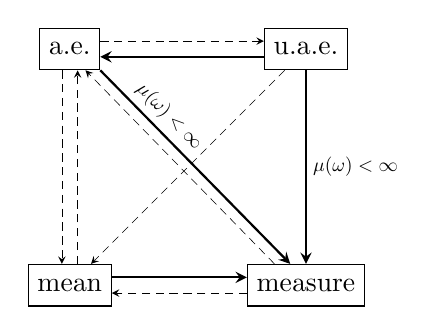
\begin{tikzpicture}
		\tikzset{
		    vertex/.style={rectangle,draw,minimum size=1.5em},
		    edge/.style={->,> = stealth, thick},
		    notimplies/.style={edge,densely dashed, very thin}
		}

		% vertices
		\node[vertex] (ae) at (0,3) {a.e.};
		\node[vertex] (uae) at (3,3) {u.a.e.};
		\node[vertex] (mean) at (0,0) {mean};
		\node[vertex] (measure) at (3,0) {measure};

		%edges
		\draw[edge] ([shift=({0,-0.1})]uae.west) -- ([shift=({0,-0.1})]ae.east) {};
		\draw[edge] ([shift=({0,0.1})]mean.east) -- ([shift=({0,0.1})]measure.west) {};
		\draw[edge] (ae.south east) -- ([shift=({-0.2,0})]measure.north) node[midway,above,sloped,rotate=0,scale=.7,pos=0.3] {$\mu(\omega)<\infty$};
		\draw[edge] (uae) -- (measure) node[midway,right,sloped,rotate=90,scale=.7] {$\mu(\omega)<\infty$};

		\draw[notimplies] ([shift=({0,0.1})]ae.east) -- ([shift=({0,0.1})]uae.west) {};
		\draw[notimplies] (uae) -- (mean) {};
		\draw[notimplies] ([shift=({0.1,0})]mean.north) -- ([shift=({0.1,0})]ae.south) {};
		\draw[notimplies] ([shift=({-0.1,0})]ae.south) -- ([shift=({-0.1,0})]mean.north) {};
		\draw[notimplies] ([shift=({0,-0.1})]measure.west) -- ([shift=({0,-0.1})]mean.east) {};
		\draw[notimplies] ([shift=({-0.4,0})]measure.north) -- ([shift=({0.2,0})]ae.south) {};

	\end{tikzpicture}
	\caption{Summary of the implication of convergences. Solid: implied (potentially under some condition specified along the line); dashed: not implied.}
\end{figure}
\FloatBarrier

To conclude our discussion we present the following result about convergence in measure.
\begin{prop}
	If $f_n\mto f$ and $f_n \mto g$, then $f=g$ a.e.
\end{prop}

The space $L^1$ belongs to the family of functional space called ``$L^p$ spaces''. In particular the distance $d_\infty(f,g) = \esssup |f - g|$ is a metric related to the space $L^\infty$, as $(L^\infty, d_\infty)$ is a metric space. A wider discussion occurs in section \vref{chapter-Lp-spaces}.

%\paragraph{The space $L^\infty$}
%
%The space $\Lc^\infty$ is the set of measurable functions that bounded a.e., namely:
%$$\Lc_\infty(\Omega, \mm, \mu) = \{f_\Omega \to \RR \text{ such that } f \text{ is measurable and essentially bounded}\}.$$
%As we have done for $\Lc^1$ we quotient set with respect to the equivalence relation $f\sim g$ if $f=g$ a.e..
%$$L_\infty(\Omega, \mm, \mu)=\frac{\Lc_\infty(\Omega, \mm, \mu)}{\sim}.$$
%
%Such set is a vector space on $\RR$ with respect to the canonical operations sum $[f]+[g]=[f+g]$ and scalar multiplication $[c f] = c[f]$, $c \in \RR$. It is also a metric space with respect to the distance $$d_\infty = \esssup_\Omega |f-g| \quad [f],[g]\in L_\infty(\Omega, \mm, \mu).$$

\paragraph{Metric convergence} 
Some convergence can be induced by a metric, in such case they are said to be \emph{metric convergences}.\\
The \textit{uniform a.e.\ convergence} is induced by the $d_\infty$ metric; indeed, we have:
$$
	d_\infty(f_n,f) 
	\to 0 
	\iff f_n 
	\uaeto f
.
$$

The \textit{convergence in mean} is a metric convergence too, as it is inducted by $d_1$:
$$
	d_1(f_n,f) 
	\to 0 
	\iff f_n 
	\lto{1} f
.
$$

The \textit{point-wise a.e.\ convergence} is not induced by any metric, so it is not a metric convergence. Some exceptions could occur, in particular when the measure $\mu$ is positive only on a countable set.

The case of \textit{measure convergence} is a bit more complicated. We have to operate on a proper space and define a proper metric.\\
Consider the measure space $(\Omega, \mm, \mu)$ where $\mu$ is finite, and the following space:
$$
	\Fc 
	\coloneqq \{f:\Omega \to \RR \text{ measurable}\}
;
$$
then consider related quotient space $\Uc \coloneqq \frac{\Fc}{\sim}$ defined with the following equivalence relation:
$$
	f
	\sim g 
	\iff 
	f
	=g 
	\quad \text{a.e.}
,
$$
that includes all the functions which are equal a.e.\ to a measurable one.
Now define the following distance:
$$
	d_\mu(f,g) 
	\coloneqq \int_\Omega \frac{|f-g|}{1+|f-g|} \; \de\mu
.$$
This is a metric in $\Uc$ and $(\Uc, d_\mu)$ is a complete metric space.\\
The measure convergence is a metric convergence with the distance $d_\mu$, namely:
$$
	d_\mu(f_n,f) 
	\to 0 
	\iff 
	f_n 
	\mto f 
	\quad \text{as } n \to +\infty
.
$$

%Uniform a.e. convergence and mean convergence are metric convergences:
%$$
%d_\infty(f_n,f) 
%\to 0 
%\iff f_n 
%\uaeto f \text{ and } d_\infty(f_n,f) \to 0 \iff f_n \lto{1} f.$$
%The point-wise a.e. convergence is not induce by any metric, while convergence in measure can be induced by a metric if $\mu(\Omega) < \infty$, and we have:
%$$\rho(f_n,f) = \int_\Omega \frac{|f_n-f|}{1+|f_n-f|} \, \de\mu \iff f_n \mto f.$$
%
%\begin{prop}
%	Consider the measure space $(\Omega, \mm, \mu)$ where $\mu$ is finite, and the following space:
%	$$\Fc \coloneqq \{f:\Omega \to \RR \text{ measurable}\}$$
%	Consider also the related quotient space $\Uc \coloneqq \frac{\Fc}{\sim}$ with the following equivalence relation:
%	$$f\sim g \iff f=g \quad \mu\text{-a.e.}$$
%	Let now:
%	$$d_\mu(f,g) \coloneqq \int_\Omega \frac{|f-g|}{1+|f-g|} \de\mu$$
%	Then $d_\mu$ is a metric in $\Uc$, $(\Uc, d_\mu)$ is a complete metric space\todo{Which $\sigma$-algebra?}, and we have:
%	$$d_\mu(f_n,f) \to 0 \iff f_n \mto f \quad \text{as } n \to +\infty$$
%\end{prop}
%The proof of the two previous results is left as an exercise for the reader.

%\begin{prop}
%	Consider the measure space of essentially bounded measurable functions $B(\Omega,\mm,\mu)$. Let:
%	$$d_B(f,g)\coloneqq\esssup_{\Omega}|f-g|$$
%	Then $d_B$ is a metric and we have:
%	$$d_B(f_n,f) \to 0 \iff f_n \uaeto f \quad \text{as } n \to +\infty$$
%\end{prop}
%
%In general, point-wise convergence is not associate with a metric, with the exception of very special cases (\textit{e.g.} $\mu$ is concentrated on a countable set).


%!!!!! once upon a time, here there was the Radon--Nikodym Derivative


\newpage
\subsection{Fundamental theorems of calculus}
%!TEX root = ../main.tex
This chapters contains the most important results of the real analysis; here we focus on calculus of one-valued functions, then, in the next chapter, we will consider also multi-valued functions. Some of those results are well-known also in lower calculus courses, but here we will approach the problem from a more technical point of view.

%This chapter is a sort of revision on the theory of function of one value. We will see the generalization of some elemental results of calculus.\\
%One of our goal is to find a link between differentiation and integration.\\
%For example consider $a,b\in \RR$, $f\in \Cc([a,b])$, and $F(x) = \int_a^x f(t) \dt$. The theorem of calculus we all know states that $F$ is differentiable in $[a,b]$ and $F'(x)=f(x)$ for all $x \in [a,b]$. How can we extend this result also to Lebesgue integrable functions?

\subsubsection{First fundamental theorem of calculus}

We try to define a generic goal. Consider the measure space $([a,b],\Lc([a,b]),\lambda)$, take $f\in L^1([a,b],\Lc([a,b]),\lambda)$ and set 
$$
	F(x) 
	= \int_a^x f(t)\dlam
,
$$
which properties does $F$ have?

\paragraph{Lebesgue points} First, our focus is on discontinuity points. The first step is to define a new notion for ``continuous points''; on those we are confident that there are no issues with integration and differentiation. 
\begin{defn}
A point $x\in[a,b]$ is a \emph{Lebesgue point} for a function $f$ if there exists a representative $\tilde{f}$ of $f$ ($\tilde f = f$ a.e.) such that:
$$
	\lim\limits_{h\to 0}
	\frac 1 h 
	\int_x^{x+h} |\tilde{f}(t) - \tilde{f}(x)|\, \dt 
	= 0
,
$$
where $h \to 0^+$ if $x=a$ or $h \to 0^-$ if $x=b$.
\end{defn}
The integral uses the $\lambda$ measure, the integral variable $t$ has been written in $\dt$ for clarity.

Notice that $\tilde{f}$ is a representative of the equivalence class $[f]$, given by almost-everywhere equality; it's typical of $\Lc^1$ spaces. 

Lebesgue points do not present discontinuity and are a sort of ``continuous points''; for instance, jump points are not a Lebesgue point; check it by considering:
$$
	f(t) = 
	\begin{cases}
		\frac{t}{|t|} & \text{if } t\in [-1,1] \setminus \{0\} \\
		0 & \text{if } t=0
	.
	\end{cases}
$$

Having checked that jumps are not Lebesgue points, one can wonder if a continuity point is a Lebesgue point. We have the following result.

\begin{theo}
	If $x_0$ is a continuity point for $f$, then $x_0$ is a Lebesgue point for $f$.
\end{theo}

\begin{proof}
	By definition of continuity:
	$$
		\forall \eps >0 \ \ \exists \, \delta :\ \ | x-x_0| < \delta \implies | f( x) -f( x_0)| < \eps ,
	$$
	we evaluate the quantity:
	$$
	\left| \frac{1}{h}\int_{x_0}^{x_0+h}| f( x) -f( x_0)| dt\right| \leq \frac{1}{| h| } \eps | \lambda ( x_0 +h-x_0)| =\frac{|h|}{|h|} \eps =\eps ,\ \forall \eps >0.
	$$
\end{proof}

\begin{theo}\label{theo-lebesgue-points}
	Let $f\in L^1([a,b],\Lc([a,b]),\lambda)$. \\
	Then almost any point $x\in[a,b]$ is a Lebesgue point of $f$. \footnotemark{}
\end{theo}
\footnotetext{For further discussion and a proof, see: W. Rudin, Real and Complex Analysis, 1987, page 138, theorem 7.6.}


\paragraph{The theorem} We are able to state a first description of the relation between differentiation and integration.
\begin{theo}[First fundamental theorem of calculus]\label{theo-first-fundamental-calculus}
	Let $f\in L^1([a,b],\Lc([a,b]),\lambda)$.\\
	The integral function $F(x) = \int_a^x f(t)$ is differentiable a.e.\ and $F'=f$ a.e. in $[a, b]$.
\end{theo}
\begin{proof}
	Let $x\in[a,b]$ be a Lebesgue point of $f$ and $h \neq 0$ such that $x+h \in [a,b]$.
	Notice that we can rewrite the value of a function in the point as follow:
	$$
		f(x) 
		= \lim\limits_{h \to 0}
		\frac 1 h 
		\int_x^{x+h} f(t) \, \dt.$$
	Consider now the incremental quotient of the integral function $F$; we need it equal to function $f$. So we write:
	$$
		\frac{F(x+h)-F(x)}{h}-f(x) 
		= \frac 1 h \int_{x}^{x+h} (f(t)-f(x)) \,\dt
	,
	$$
	then, by triangular inequality (see \vref{prop-triang-ineq-integral}), we have:
	$$
		\left| \frac{F(x+h)-F(x)}{h}-f(x) \right| 
		\leq \frac{1}{|h|} \int_x^{x+h} |f(t)-f(x)| \,\dt
	.
	$$
	Taking the limit for $h \to 0$ or $h \to 0^+$, if $x=a$, or $h \to 0^-$, if $x=b$, we have: 
	$$
		 \frac{1}{|h|} \int_x^{x+h} |f(t)-f(x)| \,\dt
		 \to 0
	.
	$$
	We have proved the theorem for any Lebesgue point, through the previous theorem (\vref{theo-lebesgue-points}) we know that the set of non-Lebesgue points has measure zero; so the thesis is proven.
\end{proof}

But this theorem opens another question: is $F$ continuous in $[a,b]$?
%!TEX root = ../main.tex
\subsubsection{Absolute continuity}
Which functions can be written as integral functions of their derivatives? In order to answer this question we must first to analyze the properties of $F$, and find a property that is stronger than simple continuity.

\begin{defn}\label{def:absolute-continuity}
	A function $f:[a,b]\to \RR$ is \emph{absolutely continuous (AC)} in $[a,b]$ if for every $\varepsilon > 0$ it exists $\delta > 0$ such that:
	$$
		\sum_{n=1}^{N} |f(b_n)-f(a_n)|
		< \varepsilon
	,
	$$
	for all $N\in \NN$, where the intervals $\{(a_n,b_n)\}_{n=1}^N$ are mutually disjoint and such that:
	$$
		\bigcup_{n=1}^{N} (a_n, b_n) 
		\subseteq [a,b] 
		\text{ and } \sum_{n=1}^{N} (b_n - a_n)
		< \delta
	.
	$$
\end{defn}

The definition still holds if $\{(a_n,b_n)\}_{n \in \NN}$ are countable. This notion is more general then uniform continuity or continuity (\vref{uniformly-continuous-functions} and \vref{continuous-functions-general} respectively), indeed the following holds:
\begin{prop}
	If $f$ is absolutely continuous in $[a,b]$, then it is also uniformly continuous in $[a,b]$.
\end{prop}
The converse is false in general, consider this function as a counterexample:
$$
	f(x) = 
	\begin{cases}
		x \sin \frac 1 x & \text{if } x \in [-1,1]\setminus\{0\}\\
		0 & \text{if } x=0
	.
	\end{cases}
$$
We see that $f$ is continuous in $[a,b]$, and thus $f$ is also uniformly continuous (see theorem \vref{Heine-Cantor-theorem}).\\
However, $f$ is not AC in $[a,b]$ by the definition.

\paragraph{Lipschitz continuity} There exists another property of continuity:
\begin{defn}\label{defn-lipschitz-continuity}
	Let $f:[a,b] \subset \RR \to \RR$. We say that $f$ is \emph{Lipschitz continuous} if exists $k > 0$ such that:
	$$
		|f(x)-f(y)| \leq k|x-y| 
		\quad \forall x,y \in [a,b]
	.
	$$
\end{defn}
Observe that the derivative of any Lipschitz continuous function is bounded.

\begin{prop}
	If $f$ is Lipschitz continuous in $[a,b]$, then it is also absolutely continuous in $[a,b]$.
\end{prop}

Again, the converse implication is not guaranteed: consider $[a,b] = [0,1]$ and $f(x)=\sqrt{x}$. While $f$ is uniformly and absolutely continuous, it is not Lipschitz continuous as $\sup_{[0,1]}f'(x)=+\infty$.

\paragraph{Summary of the continuity notions for functions} \todo{complete this with all the definitions of continuity}
\begin{itemize}
	\item The usual (strong) definition of continuity, a function $f:[a,b]\to \RR$ is continuous in $x_0$ if $\forall \eps > 0, \exists\, \delta > 0 : |x-x_{0}|<\delta \implies |f(x)-f(x_0)|<\eps$.
	\item Continuity almost everywhere, see \vref{def:continuity-almost-everywhere}.
	\item Lipschitz continuity, see \vref{defn-lipschitz-continuity}.
	\item Absolute continuity, see \vref{def:absolute-continuity}.
\end{itemize}

\paragraph{Absolute continuity of the integral}

\begin{theo} \label{theo-abs-continuity-int}
	Let $f\in L^1(\Omega, \mm, \mu)$. Then:
	$$\forall \eps > 0 \quad \exists\, \delta > 0 : \quad \int_E |f| \,\de\mu < \eps \qquad \forall E \in \mm : \ \mu(E) < \delta.$$
\end{theo}
\begin{proof}
	Let $\eps >0$. Suppose $f\geq 0$ for simplicity (otherwise is possible to use the same proof for $f^-$ and $f^+$).\\
	There exists a sequence of simple functions $\{s_n\}_{n \in \NN}$ bounded and measurable, such that $0\leq s_n \leq f$ and $s_n \lto{1} f(t)$ in $\Omega$; so (see monotone convergence \vref{monotone-convergence} or dominated convergence \vref{dominated-convergence}) there exists also a measurable and bounded function $g$ such that $$\int_E |f-g| \dmu \leq \frac \eps 2.$$
	
	Set $M=\esssup_{t\in \Omega}|g(t)|>0$ and $\delta=\frac{\eps}{2M}$. Then:
	$$
		\int_E |f| \dmu 
		\leq \int_E |f-g| \dmu + \int_E |g| \dmu 
		< \frac{\eps}{2} + M\mu(E)
		< \frac{\eps}{2} + M\delta
		= \frac{\eps}{2} + M\frac{\eps}{2M}
		= \eps
	$$
	with $\mu(E) < \delta$.
\end{proof}

This corollary applies the previous theorem to the case of the integral function:
\begin{coro} \label{absolute-continuity-integral}
	Let $f\in L^1 ([a,b], \Lc[a,b],\lambda)$, and set:
	$$F(x) = \int_a^x f(t) \,\dlam.$$
	Then the integral function $F$ is absolutely continuous in $[a,b]$.
\end{coro}
\begin{proof}
	Fix $\eps> 0$ and let $\delta > 0 $ given by the previous theorem \vref{theo-abs-continuity-int}. \\
	Let also $N\in\NN$, and $\{(a_n,b_n)\}_{n=1:N }\subset [a,b]$ be a collection of mutually disjoint intervals such that $\sum_{n=1}^{N}(b_n-a_n)< \delta$ and $E=\bigcup_{n=1}^{N} (a_n,b_n)$ with $\lambda(E)<\delta$.\\
	Then we have:
	$$\sum_{n=1}^N |F(b_n)-F(a_n)| 
	= \sum_{n=1}^N \left| \int_{a_n}^{b_n} f(t) \,\dlam \right|
	\leq \sum_{n=1}^N \int_{a_n}^{b_n}|f(t)| \,\dlam
	= \int_E |f(t)| \,\dlam < \eps.$$
	Thus, by the definition, $F$ is absolutely continuous in $[a,b]$.
\end{proof}

For example take $f(t)= \frac 1 {2\sqrt{t}}\in \Lc^1([0,1],\Lc([0,1]),\lambda)$; then we have:
$$ \int_0^x \frac 1 {2\sqrt{t}} \dlam = \sqrt{x}.$$
Thanks to the previous theorem we have that $\sqrt{x}$ is absolutely continuous in $[0,1]$. However we already know that it is not Lipschitz-continuous.

\paragraph{The space of absolute continuous functions} It is easy to see that the set of the function which are absolute continuous on a closed interval is closed with respect to sum and scalar product. Indeed, if $f$ and $g$ are absolutely continuous in $[a,b]$, then $\alpha f + \beta g$ is absolutely continuous too. So the space $$AC([a,b])\coloneqq \{f:[a,b] \to \RR : f  \ AC\text{ in } \Omega\},$$ is a vector space on $\RR$ with respect to the canonical operations.


%!TEX root = ../main.tex
\subsubsection{Second fundamental theorem and bounded variation functions}

We know that if $f\in L^1([a,b], \Lc[a,b], \lambda)$, then $F(x)=\int_0^x f(t) \dt$ is such that $F\in AC([a,b])$ and $F'=f$ a.e. in $[a,b]$.

How can we find, given the functions $F:[a,b]\to \RR$, a complete characterization\footnote{A full characterization means a condition which is necessary and sufficient.} of the following \emph{calculus formula}?

$$F(x)=F(a)+\int_a^x F'(t) \dt \qquad \forall x\in [a,b]$$

These are some necessary conditions:
\begin{itemize}
	\item $F' \in L^1([a,b],\Lc[a,b],\lambda);$
	\item $F \in AC([a,b]).$
\end{itemize}
Now we try to figure out it those conditions can be also sufficient. But first consider these two example.\\
Look at this function: $$F(x)=\begin{cases}
x^2 \sin(\frac{1}{x^2}) &x\in[-1,1] \setminus \{0\}\\
0 &x=0.
\end{cases}$$
The function $F$ is differentiable in $[-1,1]$ but $F'\notin L^1([-1,0])$.

Consider: $$F(x) = \begin{cases}
-1 &x\in [0,1]\\
1&x\in[-1,0)
\end{cases}$$
It is differentiable in $[1,1]$ and $F'=0 \in L^1([-1,1])$, but the calculus formula doesn't hold.

The characterization we are looking for is given by the following theorem:
\begin{theo}[Second fundamental theorem of calculus]   \label{theo-2nd-found-calc}
	A function is absolutely continuous if and only if it is differentiable a.e. in $[a,b]$, its derivative belongs to $L^1$ and for such function holds the calculus formula. Namely:
	$$F\in AC([a,b]) \iff
	\begin{cases}
	F \text{ is differentiable a.e. in } $[a,b]$; \\
	F'\in L^1 ([a,b],\Lc[a,b],\lambda); \\
	F(x) = F(a)+\int_a^x F'(x) \, \dlam \quad \forall x \in [a,b].
	\end{cases}
	$$
\end{theo}
The \textit{sufficient condition} ($\implies$) part is already proven. 


\paragraph{Bounded variation functions} To provide also a demonstration of the necessary part we have to introduce a new class of function.
\begin{defn}
	Given a function $f:[a,b] \subset \RR \to \RR$, and $x,y\in [a,b]$ such that $x<y$, the \emph{total variation} of $f$ in $[x,y]$ is defined as follows:
	$$
	\tv^y_x(f) 
	\coloneqq \sup_{\{t_i\}} \sum_{n=1}^{N}|f(t_n)-f(t_{n-1})|
	,
	$$
	where $x<t_0<t_1<\cdots<t_N<y$.
	
	The function $f$ is said to be a \emph{bounded variation function} in $[a,b]$ if $\tv^b_a (f) < +\infty$.
\end{defn}

Notice that a function $f$ is not a bounded variation function if and only if there exists $x \in (a,b]$ such that $\tv^x_a (f) = +\infty$: intuitively, the total variation quantifies jumps and oscillations of the function.

A sufficient condition for bounded variation is the monotonicity on an interval. Indeed, $\tv_a^b = f(b)-f(a)$ is non-decreasing or $\tv_a^b=f(a)-f(b)$ is non-increasing.
\begin{figure}[htpb]
	\centering
	\tikzset{every picture/.style={line width=0.75pt}} %set default line width to 0.75pt

	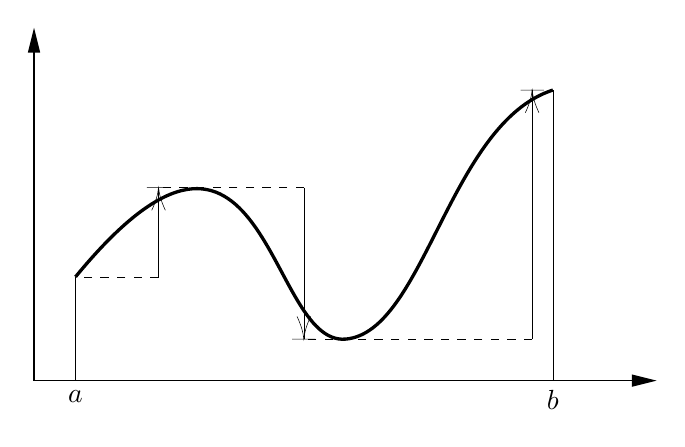
\begin{tikzpicture}[x=0.75pt,y=0.75pt,yscale=-1,xscale=1]
	%uncomment if require: \path (0,303); %set diagram left start at 0, and has height of 303

	\draw [very thick](180,160) .. controls (272,48.03) and (272,193) .. (310,190) .. controls (348,187) and (360,86.03) .. (410,70);
	\draw [very thin](180,160) -- (180,210);
	\draw [very thin](410,70) -- (410,210);
	\draw [very thin] (220,160) -- (220,117);
	\draw [shift={(220,117)}, rotate = 90] [very thin] (0,5.59) -- (0,-5.59)(10.93,-3.29) .. controls (6.95,-1.4) and (3.31,-0.3) .. (0,0) .. controls (3.31,0.3) and (6.95,1.4) .. (10.93,3.29);
	\draw (160,210) -- (160,42);
	\draw [shift={(160,40)}, rotate = 90] [fill={rgb, 255:red, 0; green, 0; blue, 0 } ][line width=0.08] [draw opacity=0] (12,-3) -- (0,0) -- (12,3) -- cycle;
	\draw (160,210) -- (458,210);
	\draw [shift={(460,210)}, rotate = 180] [fill={rgb, 255:red, 0; green, 0; blue, 0 } ][line width=0.08] [draw opacity=0] (12,-3) -- (0,0) -- (12,3) -- cycle;
	\draw [very thin] (290,117) -- (290,190);
	\draw [shift={(290,190)}, rotate = 270] [very thin] (0,5.59) -- (0,-5.59)(10.93,-3.29) .. controls (6.95,-1.4) and (3.31,-0.3) .. (0,0) .. controls (3.31,0.3) and (6.95,1.4) .. (10.93,3.29);
	\draw [dashed, very thin] (220,160) -- (180,160);
	\draw [dashed, very thin] (290,117) -- (220,117);
	\draw [dashed, very thin] (400,190) -- (290,190);
	\draw [very thin] (400,190) -- (400,70);
	\draw [shift={(400,70)}, rotate = 90] [very thin] (0,5.59) -- (0,-5.59)(10.93,-3.29) .. controls (6.95,-1.4) and (3.31,-0.3) .. (0,0) .. controls (3.31,0.3) and (6.95,1.4) .. (10.93,3.29);
	%\draw [line width=0.75] (470,160) -- (470,70);
	%\draw [shift={(470,70)}, rotate = 90] [line width=0.75] (0,5.59) -- (0,-5.59);
	%\draw [shift={(470,160)}, rotate = 90] [line width=0.75] (0,5.59) -- (0,-5.59);

	\draw (180,210) node [below] {$a$};
	\draw (410,210) node [below] {$b$};
	%\draw (476,102.4) node [anchor=north west][inner sep=0.75pt] {$=\mathrm{V}_{a}^{b}$};
	\end{tikzpicture}
\end{figure}
\FloatBarrier

Let us consider some properties.
\begin{prop}
	Let $f$ be a bounded variation function in $[a, b]$.\footnotemark{} Then:
	$$
	\tv^b_a(f) 
	= \tv^c_a(f) + \tv^b_c(f) 
	\quad \forall c \in [a,b].$$
	Moreover the operator $x\mapsto \tv^x_a(f)$ is non decreasing, \textit{i.e.}:
	$$\tv^y_a(f) -\tv^x_a(f) = \tv^y_x(f) \geq 0 \quad \forall x,y: y>x.$$
\end{prop}
\footnotetext{For further discussion, see: A. N. Kolmogorov, S. V. Fomin, Introductory Real Analysis, 1975, page 329, theorem 2.}

Observe that the total variation is \textit{absolute homogeneous}:
$$
\forall c \in \RR 
\quad \tv^y_x(cf)
= \abs{c} \tv^y_x(f)
.
$$

\paragraph{The space of bounded variation functions and the relation with absolute continuous ones} It is easy to see that the set of the bounded variation function on a closed interval is closed with respect to sum and scalar product:
$$BV([a,b])\coloneqq \{G:[a,b]\to \RR : \tv^b_a (G) < \infty\}.$$
 Indeed, if $f$ and $g$ are bounded variation in $[a,b]$ and $\alpha \in \RR$, then:
$$\tv_a^b(\alpha f) = \abs\alpha \tv_a^b(f) \text{ and } \tv_a^b(f+g)= \tv_a^b(f)+\tv_a^b(g).$$

Remember that this point was made also for absolute continuous functions: the spaces of functions with these properties are vector spaces.\\
Also there is a strong relation between these two properties:

\begin{prop}\label{AC-implies-BV} \label{prop-ac-implies-bv}
	If a function $f$ is absolute continuous in $[a, b]$ then it is also bounded variation in $[a, b]$ and $x\mapsto \tv^x_a(f)$ is absolute continuous in $[a, b]$.\footnotemark{}\\
	Namely:
	$$
	f\in AC([a,b]) \implies \begin{cases}
	f \in BV([a,b])\\
	\tv_a^x(f) \in AC ([a,b]).
	\end{cases}
	$$
\end{prop}
\footnotetext{For further discussion, see: A. N. Kolmogorov, S. V. Fomin, Introductory Real Analysis, 1975, page 337, theorem 2.}

\paragraph{Relations with monotonicity and continuity} This new class of function is related to many well-known properties.

In general, uniform continuity does not imply bounded variation; consider the following example:
$$f(x) = \begin{cases}
x \cos \frac 1 x & x \in (0,1] \\
0 & x=0.\end{cases}$$
This function is uniformly continuous in $[0,1]$ (see Heine--Cantor's theorem \vref{Heine-Cantor-theorem}), but it is not bounded variation in $[0,1]$: prove it using the definition on a suitable partition of such interval. Note also that the length of the graph of $f$ is not finite.

Remember that a sufficient condition for bounded variation is the monotonicity on an interval. Moreover, we have the following proposition:
\begin{prop} \label{theo-bv-non-decreasing}
	Every bounded variation function can be written as a difference of two non-decreasing functions.
\end{prop}
\begin{proof}
	Observe that $f(x)=\tv^x_a(f) -[\tv^x_a(f) - f(x)]$. \\ 
	Taking $v(x) = \tv^x_a-f(x)$, by definition of total variation we have:
	$$v(y)-v(x) = \tv_x^y (f) - (f(y)-f(x)) \geq 0 \quad \text{with }y>x$$
	since the total variation can be equal to the jump between $x$ and $y$ (if $f$ is monotone) or greater\footnote{Think, for instance, if it jumps in between.}; and thus $v(x)$ is non-decreasing.
\end{proof}

Due to this fact we understand that every bounded variation function has at most a countable set of jump discontinuities; so those function are Lebesgue-integrable! Namely if $f\in BV([a,b])$ then $f\in L^1([a,b])$.

%Thus such functions are Riemann-integrable where they are bounded variation. Now you reader should motivate why...\\

\begin{theo}
	Any monotone function in $[a,b]$ has finite derivative a.e. in $[a,b]$.\footnotemark
\end{theo}
\footnotetext{For further discussion, see: A. N. Kolmogorov, S. V. Fomin, Introductory Real Analysis, 1975, page 321, theorem 6.}
\begin{coro}\label{coro-deriv-bv}
	Any $f \in BV([a,b])$ has finite derivative a.e. in $[a,b]$. Moreover $f'\in L^1([a,b])$.
\end{coro}

Moreover we have:
\begin{prop}\label{prop-nondecreasing-inequality}
	Let $f: [a,b]\to \RR$ be a non-decreasing function. Then its derivative $f' \in L^1([a,b])$ and we have:
	$$\int_a^b f'(t) \,\dt \leq f(b)- f(a).$$
\end{prop}
\begin{proof}
	Set:
	$$\Phi_n(t) = n \left[ f\left( t + \frac 1 n \right)-f(t) \right]$$
	with $n \in \NN_0$. We extend $f$ after $b$, considering $f(t)=f(b) \ \forall t \in [b,b+\frac 1 n]$.
	
	As $f\in L^1([a,b])$ also $\Phi_n \in L^1([a,b]) \ \forall n \in \NN_0$; and $f'(t) = \lim\limits_{n \to \infty}\Phi_n(t)$ for almost any $t \in [a,b]$ (convergence almost everywhere).\\
	Then we have:
	\begin{align*}
	\int_a^b \Phi_n (t) \,\dt
	&= n \int_a^b \left[ f\left( t + \frac 1 n \right)-f(t) \right] \,\dt
	&(\tau \coloneqq t+ \tfrac 1 n) \\
	&= n\left[\int_{a+\frac 1 n}^{b + \frac 1 n} f(\tau) \,\dt - \int_a^b f(t) \,\dt\right] \\
	&= n\left[\int_{b}^{b + \frac 1 n} f(t) \,\dt - \int_a^{a+\frac 1 n} f(t) \,\dt\right]
	&\text{(monotonicity)} \\
	&\le n f(b) \frac 1 n - n f(a) \frac 1 n
	= f(b) - f(a).
	\end{align*}
	
	We now apply Fatou's lemma, and thus we have:
	\begin{align*}
	\int_a^b f'(t) \,\dt
	&= \int_a^b \lim_{n \to \infty}\Phi_n(t) \,\dt\\
	&\leq \liminf_{n \to \infty} \int_a^b \Phi_n(t) \,\dt \\
	&\leq \int_a^b \Phi_n(t) \,\dt\\
	&\leq f(b) - f(a).
	\end{align*}
	
	Thus $\int_a^b f'(t) \leq f(b)- f(a)$ and $f' \in L^1([a,b])$.
\end{proof}

Observe that the inequality can be strict. Indeed, take:
$$f(x) = \begin{cases}
0 & x\in[0,\frac 1 2) \\
1 & x \in [\frac 1 2, 1];
\end{cases}$$
in this case we get: $\int_0^1 f'(t)\dt = 0 < 1 = f(1) - f(0)$.

The following last theorem provides a sort of generalization of the characterization of the constant function.\footnote{For further discussion see: A. N. Kolmogorov, S. V. Fomin, Introductory Real Analysis, page 339}
\begin{theo} \label{theo-deriv-zero-non-decr-constant}
	Let $G\in AC([a,b])$ be non-decreasing and such that $G'=0$ a.e. in $[a,b]$. \\
	Then $G$ is constant in $[a,b]$.
\end{theo}
The proof of this result is very hard.

\paragraph{Proof of the second fundamental theorem} Now we prove theorem \vref{theo-2nd-found-calc}. The \textit{sufficient condition} part is already proven. We need to prove that if $F \in AC([a,b])$ then $F$ is differentiable a.e. in $[a,b]$, its derivative $F' \in L^1([a,b])$ and the calculus formula holds.
\begin{proof}
	\textit{Necessary condition} $\impliedby$:\\
	Consider a function $F \in AC([a,b])$, we have that (see proposition \vref{theo-bv-non-decreasing} and \vref{prop-ac-implies-bv}):
	$$F=F_1 - F_2 = \tv_a^x (F) - [\tv_a^x(F)-F];$$
	where $F_1, f_2$ are $AC([a,b])$ and non-decreasing.
	
	Thus we can suppose that $F$ is non-decreasing without loss of generality, and prove the theorem in the general case by linearity.\\
	Then, thanks to Corollary \vref{coro-deriv-bv} we have that $F$ is differentiable a.e. in $[a,b]$ and $F' \in L^1([a,b])$.\\
	Now it remains to prove the calculus formula. 
	
	Set:
	$$\Phi(x) = F(x)-\int_a^x F'(t) \,\dt \quad \forall x \in [a,b],$$
	it is $AC([a,b])$. Moreover, since $F$ is non-decreasing, thanks to \vref{prop-nondecreasing-inequality} we have that for all $x_1, x_2 \in [a,b]$ such that $x_1 \leq x_2$:
	$$\Phi(x_1)-\Phi(x_2) = F(x_1)-F(x_2) - \int_{x_1}^{x_2}F'(t) \, \dt \geq 0,$$
	so also $\Phi$ is non-decreasing.
	
	Using the first fundamental theorem of calculus (\vref{theo-first-fundamental-calculus}), we have that $\Phi'=0$ a.e. in $[a,b]$. Then (\vref{theo-deriv-zero-non-decr-constant}) $\Phi$ is constant everywhere in $[a,b]$, namely $\Phi(x)=c$ for any $x\in [a,b]$. Take $x = a$, then $F(a) = c$, and thus:
	$$F(x)=F(a) + \int_a^x F'(t) \,\dt.$$
\end{proof}

Notice that the first theorem was proven with the Lebesgue's point and it was quite trivial. Now we stated that absolute continuity is necessary for the calculus formula.

This is a complete characterization of AC functions: being $L^1$ is not enough for a function to be reconstructed.\\
This theorem is the largest generalization of the calculus formula currently existing.

%!TEX root = ../main.tex
\subsubsection{Further results}

\paragraph{A general version of the change of variable} With this new knowledge we can improve our tools:
\begin{theo}
	Consider a function $g:[a,b]\to [c,d] \in AC([a,b])$, such that it is strictly monotone.\\
	Then, for any $f:[c,d] \to \infty \in L^1([c,d])$ then:
	$$\int_c^d f(t) \, \dt =  \int_a^b f(g(\tau))|g'(\tau) \,\dt = \int_a^b f(g(\tau))\,\de \mu$$
	where $\frac{\de \mu}{\de \tau} = |g'|$, the Radon--Nikodym derivative.
\end{theo}

Notice that the fact that the composition of function is still Lebesgue-integrable is a part of the theorem: the compound function$(f\circ g)|g'|$ is measurable and integrable as a consequence of the assumptions, indeed we have:
$$f \in L^1([c,d]) \iff (f\circ g)|g'|\in L^1([a,b]).$$
The theorem also holds for $f$ just measurable and non-negative. In this case, $f$ is integrable in $[c,d]$ if and only if $(f\circ G) \, |G'|$ is integrable in $[a,b]$.


\paragraph{A sufficient condition for absolute continuity} The following result holds\footnote{For further discussion, see: W. Rudin, Real and Complex Analysis, 1987, page 149, theorem 7.21.}:
\begin{theo}
	Let $f:[a,b]\in\RR \to \RR$. If $f$ is differentiable everywhere in $[a,b]$ and $f' \in L^1([a,b])$, then $f \in AC([a,b])$.
\end{theo}

Consider for example the following function:
$$f(x) = \begin{cases}
x^{\frac 3 2} \sin \frac 1 x & \text{if }x \in \left(0,1\right]\\
0& \text{if }x=0.
\end{cases}$$
Its derivative exists everywhere:
$$f'(x)= \begin{cases}
\frac 3 2 \sqrt x \sin \frac 1 x - \frac {1}{\sqrt{x}} \cos \frac 1 x & \text{if }x\in\left(0,1\right] \\
0 & \text{if }x=0;
\end{cases}$$
In $0$ we computed separately: $\frac{f(h)-f(0)}{h} = \frac{h^{\frac 3 2 } \sin \frac 1 h }{h} \to 0$ for $h \to 0^+$.\\
So $f'$ is not continuous, but it is integrable in $([0,1])$, and thus $f \in AC([0,1])$. Observer also that $f$ is not lipschitz continuous.

What if we have that $f$ is continuous, $f'$ exists a.e., and $f'$ is integrable in $[a,b]$? In this case $f$ might not be $AC([a,b])$: consider for example the Vitali--Cantor function (see definition \vref{Vitali-Cantor-function}).

\paragraph{Comparison between Lebesgue and Riemann integral} There are plenty of definitions for integrals: now we make a comparison between the two integral that we already know. Consider, in this paragraph, the space $(\RR, \Lc(\RR), \lambda)$.
\begin{theo}
	Let $f:(a,b)\subset \RR \to \RR$ bounded. \\
	Then $f$ is Riemann-integrable in $(a,b)$ if and only if $f$ is continuous a.e. in $(a,b)$.
\end{theo}\footnote{For further discussion, see: W. P. Ziemer, Modern Real Analysis, 2017, page 153, theorem 6.19.}

Notice for example that $\Ind_{\QQ \cap (a,b)}$ is not Riemann integrable, because it is nowhere continuous. But $\Ind_{\QQ \cap (a,b)}=0$ a.e. in $(a,b)$, it is Lebesgue-integrable, and $\int_a^b \Ind_{\QQ \cap (a,b)} \dlam =0$.

More in general, if $f: (a,b) \to \RR$ is Lebesgue-measurable and bounded, then $f$ is Lebesgue integrable: indeed, $f$ is measurable.

\begin{theo}
	Let $f:(a,b)\subset \RR \to \RR$ be bounded and continuous a.e. in $(a,b)$. Then the Riemann integral and the Lebesgue integral coincide,\footnotemark{} namely:
	$$ \underbrace{\int_a^b f(t) \,\dt}_{\text{Riemann}}
	= \underbrace{\int_a^b f(t) \,\dlam}_{\text{Lebesgue}}.$$
\end{theo}
\footnotetext{For the proof, see: A. N. Kolmogorov, S. V. Fomin, Introductory Real Analysis, 1975, pages 309-310, theorem 4.}

Consider for example the generalized Cantor set $T_\varepsilon$ of Lebesgue measure $3\frac{1-\varepsilon}{3-2\varepsilon}$. Then $\Ind_{T_\varepsilon}$ is bounded but it is not Riemann integrable since it's discontinuities at each point. Indeed, the interior of $T_\varepsilon$ is empty and $\Ind_{T_\varepsilon}$ has no limit as $x\to x_0$ for any $x_0 \in T_\varepsilon$. Moreover $\Ind_{T_\varepsilon}$ is Lebesgue integrable in $[0,1]$ but it is not equal almost everywhere to any Riemann integrable function.

Let us now focus on improper Riemann integrals:
\begin{theo}
	Let $f: (a,b) \subseteq \RR \to \RR$, with $a,b\in \RR^\star : a< b$.\\
	If $f$ is Riemann integrable in $(a,b)$ in the improper sense and it changes its sign at most a finite number of times, then $f$ is Lebesgue integrable in $(a,b)$ and the two integrals coincide.
\end{theo}

If $f$ changes sign an infinite number of times then the Riemann improper integral can exists but $f$ might not be Lebesgue measurable. Consider the following function:
$$f(t)
=\frac {\sin t}{t}
\quad t \in (0,+\infty).$$
Then $f$ is Riemann-integrable as $\lim\limits_{a \to +\infty} \int_0^a f(t) \,\dt$ exists. However, it is not integrable, indeed:
$$ \int_0^{+\infty} \left| \frac{ \sin t}{t} \right| \dlam 
= \int_0^{+\infty}\frac 1 t \dlam
= +\infty.$$
	
\begin{proof}
	Suppose $f>0$. We can find two sequences, $\{a_n\}_{n\in \NN}$ and $\{b_n\}_{n\in \NN}$, such that $a_n < b_n$, $a_n \downarrow a$, $b_n \uparrow b$, and $(a,b)=\bigcup_{n\in \NN} (a_n,b_n)$. Suppose $f$ is bounded on $(a_n,b_n) \ \forall n \in \NN$.\\
	Therefore $f$ is Riemann integrable on each $(a_n,b_n)$ and we have:
	$$\underbrace{\int_{a_n}^{b_n} f(t) \,\dt}_{\text{Riemann}}
	= \underbrace{\int_{a_n}^{b_n} f(t) \,\dlam}_{\text{Lebesgue}}
	\quad \forall n \in \NN.
	$$
	Set $F_n = \bigcup_{j=0}^n (a_j,b_j)$ and $f_n = f \Ind_{F_n}$. Then $f_n \uparrow f$ and, using monotone convergence, we have:
	$$\lim_{n \to \infty} \int_a^b f_n(t) \,\dlam
	= \lim_{n \to \infty} \int_{a_n}^{b_n} f(t) \,\dlam
	= \int_a^b f(t) \,\dlam.
	$$
	By definition of Riemann improper integral, we have:
	$$\int_a^b f(t) \,\dt
	= \lim_{n \to \infty} \int_{a_n}^{b_n} f(t) \,\dt.
	$$
	Putting all together, we get the thesis:
	$$\lim_{n \to \infty} \int_a^b f_n(t) \,\dlam 
	= \lim_{n \to \infty} \int_{a_n}^{b_n} f(t) \,\dt.
	$$
\end{proof}

Consider now some examples: the function
$$f(t)=\begin{cases}
	\sin(t) & \text{if } t \in \RR \setminus \ZZ \\ 
	+ \infty & \text{if } t \in \ZZ^+ \\ 
	- \infty & \text{if } t \in \ZZ_-	
	\end{cases} $$
 is essentially bounded and continuous a.e. in $\RR$, and $f(t) = \sin(t)$ a.e. in $\RR$.

The function
	$$f(t)=\begin{cases} 
	\sin(t) 		& \text{if } t \in \left[0,1\right]\cap \left(\RR \setminus \QQ \right) \\
	+ \infty 	   &  \text{if } t \in \left[0,1\right]\cap \QQ
	\end{cases}$$
is nowhere continuous, bounded, and measurable. Then that $f$ is Lebesgue integrable, hence $\int_0^1 f(t) \,\dlam$ exists finite.\\
Indeed, $f(t) = \sin (t)$ $a.e.$ in $\left[0,1\right]$, thus:
	$$\int_0^1 f(t) d \lambda =\underbrace{\int_0^1 \sin t \,\dlam}_{\text{Lebesgue}}
	=\underbrace{\int_0^1 \sin t \,\dt}_{\text{Riemann}}.$$


\paragraph{Lebesgue decomposition of bounded variation functions} Any bounded variation function can be written as a sum of three proper function. Let's understand what kind of function they are.

\begin{defn}
	Let $\{x_n\}_{n\in\NN}$ and $\{x_n'\}_{n\in\NN}$ be two sequences of points in $[a,b]$. \\
	Let also $\{h_n\}_{n\in\NN}$, $\{h_n'\}_{n\in\NN} \subset \RR$ such that:
	$$
	\sum_{n\in\NN} |h_n| 
	< +\infty, 
	\qquad \sum_{n\in \NN}|h_n'| 
	< +\infty
	.
	$$
	A function $f$ is called \emph{jump function} if it can be written as:
	$$
	f(x) 
	= \sum_{\substack{n \in \NN:\\ x_n \vphantom{x_n' \le} < x }} h_n 
	+ \sum_{\substack{n \in \NN:\\ x_n'\le x}} h'_n
	.$$
\end{defn}


Notice that the first sum generates a function continuous from the left, the other one from the right.

Jump functions are step function if the sequences $\{x_n\}$ and $\{x'_n\}$ are strictly increasing, but jump functions can be more general.

There is another more explanatory form for writing a jump function $f:[a,b] \to \RR$ where $f(a)=0$. In such case we would have:
$$f(x) = \sum_{n\in\NN}g_n(x) + \sum_{n\in\NN}g'_n(x),$$
where:
$$ g_n(x) = \begin{cases}
0 & a \leq x \leq x_n\\
h_n & x_n < x \leq b
\end{cases} \qquad 
g'_n(x)= \begin{cases}
0 & a \leq x < x'_n\\
h'_n & x_n \leq x \leq b.
\end{cases}
$$

We can provide some example of jump functions. For instance we can define a jump function on $[0,1]$ by setting $x_n=\frac 1 n$ and $h_n = \frac{(-1)^n}{n^{\frac 3 2}}$ with $n \in \NN_0$.
In that case we have $f(\frac{1}{100}) = \sum_{n=101}^{+\infty} \frac{(-1)^n}{n^{\frac 3 2}}$ or $f(\frac{1}{\sqrt{71}}) = \sum_{n=8}^{+\infty} \frac{(-1)^n}{n^{\frac 3 2}}$.

Here an example of a jump function which is not a step function; let $\{x_n\}_{x \in \NN}$ be an enumeration of $\QQ$, and set $h_n = \frac 1 {2^n}$. Thus our function is:
	$$f(x)=\sum_{x_n < x} \frac 1 {2^n}.$$
It can be proven that $f$ is discontinuous at any $x \in \QQ$ and continuous at any $x \in \RR \setminus \QQ$.\footnote{For further discussion, see: A. N. Kolmogorov, S. V. Fomin, Introductory Real Analysis, 1975, pages 315-327.}


Observe that any jump function $f:[a,b] \to \RR$ belongs to $BV([a,b])$,\footnote{What is its total variation?} therefore it is differentiable a.e. in $[a,b]$ and its derivative is zero a.e.. Moreover, as they are bounded, they are also Lebesgue-integrable. 

There exists non-constant functions $f:[a,b] \to \RR$ which are continuous, non-decreasing with zero derivative a.e.; such functions are $BV$ but not $AC$ since the Calculus formula doesn't hold. A counterexample is again the Vitali--Cantor function (see definition \vref{Vitali-Cantor-function}).

Thinking to such counterexample, we can define another kind of function.
\begin{defn}
	A non constant function $f:[a,b] \subset \RR \to \RR$ is a \emph{singular function} (or Cantor-like function) if:
	\begin{itemize}
		\item $f$ is continuous in $[a,b]$;
		\item $f$ is non-decreasing;
		\item $\exists \, f'$ a.e. and $f'=0$ a.e. in $[a,b]$.
	\end{itemize}
\end{defn}

We see lot of kinds of functions: they are somehow related by the following result.
\begin{theo}[Lebesgue decomposition of bounded variation functions]
	Let $f\in BV([a,b])$. Then there exist three functions:
	\begin{itemize}
		\item a function $\phi_1 \in AC([a,b])$;
		\item a singular function $\phi_2$;
		\item a jump function $\phi_3$
	\end{itemize}
	such that $$f= \phi_1+\phi_2+\phi_3 \text{ in }[a,b].$$
\end{theo}\footnote{For further discussion, see: G. Leoni, A First Course in Sobolev Spaces, 2017, page 104, theorem 3.89.}

Notice that, if $f\in BV([a,b])$, then $f'=\phi_1'$ a.e. in $[a,b]$. Thus, as we already know, we cannot in general reconstruct a bounded variation function by integrating its derivative: the calculus formula only reconstructs the $AC$ function of the Lebesgue decomposition, see that if $f' = \phi'_1$ a.e. in $[a,b]$ then: $$\int_a^x f'(t) \dt = \phi_1(x) - \phi_1(a).$$


\newpage
\subsection{Integrals on product spaces}
%!TEX root = ../main.tex
\subsubsection{Product measures}
\todo{part of this can be taken as intro of the subsection.}
In this section we discuss on how to measure a function which domain is not mono-dimensional.
We know yet how the Riemann integration has solved this problem:

%\missingfigure{Here we should put an image of Riemann in $\RR^2$ measure with axis and a proper patatoide.}
\begin{figure}[htpb]
	\centering
	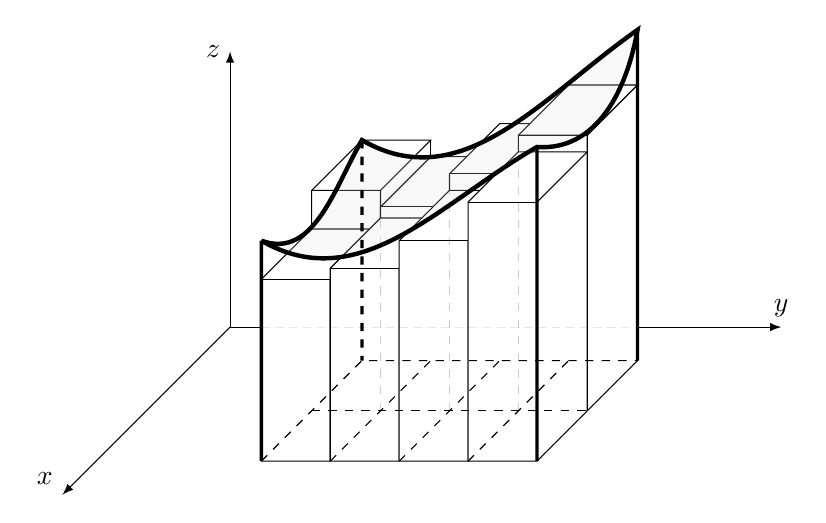
\begin{tikzpicture}[y={(0:1cm)},x={(225:0.86cm)}, z={(90:1cm)},yscale=0.7,xscale=0.7]

	% coordinates for the lower grid
	\path
	  (1,3,0) coordinate (bm0) -- 
	  (4,3,0) coordinate (fm0) coordinate[midway] (lm0) --
	  (4,8,0) coordinate[pos=0.25] (fm1) coordinate[midway] (fm2) coordinate[pos=0.75] (fm3) coordinate (fm4) --
	  (1,8,0) coordinate (bm4) coordinate[midway] (lm4)--
	  (bm0) coordinate[pos=0.25] (bm3) coordinate[midway] (bm2) coordinate[pos=0.75] (bm1);
	\draw[dashed]
	  (lm0) -- 
	  (lm4) coordinate[pos=0.25] (lm1) coordinate[midway] (lm2) coordinate[pos=0.75] (lm3);

	% the blocks
	\DrawBlock{b}{1}{4}
	\DrawBlock{b}{2}{3.7}
	\DrawBlock{b}{3}{4.3}
	\DrawBlock{b}{4}{5}
	\DrawBlock{f}{1}{3.3}
	\DrawBlock{f}{2}{3.5}
	\DrawBlock{f}{3}{4}
	\DrawBlock{f}{4}{4.7}

	\foreach \Point/\Height in {lm1/3.7,lm2/4.3,lm3/5}
	  \draw[ultra thin,dashed,opacity=0.2] (\Point) -- ++(0,0,\Height);

	% the lower grid
	\foreach \x in {1,2,3}
	  \draw[dashed] (fm\x) -- (bm\x);
	\draw[dashed] (fm0) -- (bm0) -- (bm4);
	\draw (fm0) -- (fm4) -- (bm4);
	\draw[dashed] (lm0) -- (lm4);

	% coordinates for the surface
	\coordinate (curvefm0) at ( $ (fm0) + (0,0,4) $ );
	\coordinate (curvebm0) at ( $ (bm0) + (0,0,4) $ );
	\coordinate (curvebm4) at ( $ (bm4) + (0,0,6) $ );
	\coordinate (curvefm4) at ( $ (fm4) + (0,0,5.7) $ );

	% the surface
	\filldraw[ultra thick,fill=gray!25,fill opacity=0.2]
	  (curvefm0) to[out=-30,in=210] 
	  (curvefm4) to[out=-4,in=260]
	  (curvebm4) to[out=215,in=330]
	  (curvebm0) to[out=240,in=-20]
	  (curvefm0);

	% lines from grid to surface
	\draw[very thick,name path=leftline] (curvefm0) -- (fm0);
	\draw[very thick] (curvefm4) -- (fm4);
	\draw[very thick,name path=rightline] (curvebm4) -- (bm4);
	\draw[very thick,dashed] (curvebm0) -- (bm0);

	% coordinate system
	\coordinate (O) at (0,0,0);
	\draw[-latex] (O) -- +(5,0,0) node[above left] {$x$};
	\path[name path=yaxis] (O) -- +(0,10,0) coordinate (yaxisfinal) node[above] {$y$};
	\draw[-latex] (O) -- +(0,0,5) node[left] {$z$};
	\path[name intersections={of=yaxis and leftline,by={yaxis1}}];
	\path[name intersections={of=yaxis and rightline,by={yaxis2}}];
	\draw (O) -- (yaxis1);
	\draw[densely dashed,opacity=0.1] (yaxis1) -- (yaxis2);
	\draw[-latex] (yaxis2) -- (yaxisfinal);

	% for debugging
	%\foreach \Name in {bm0,fm0,lm0,fm1,fm2,fm3,fm4,bm4,lm4,bm1,bm2,bm3,lm1,lm2,lm3,%
	%curvefm0,curvebm0,curvebm4,curvefm4}
	%  \node at (\Name) {\Name};  
	\end{tikzpicture}
\end{figure}
\FloatBarrier

The main idea is to calculate the integral through what we know in one dimension, using the techniques for the integration of one variable:
$$\iint_\Omega f(x,y) \dx \dy=\int_a^b \left( \int_{\Omega_x} f(x,y) \dy \right) \dx=\int_c^d \left( \int_{\Omega_y} f(x,y) \dx \right) \dy$$

Now we need to extend this to the Lebesgue and abstract integral. This technique should be extended to proceed for a very general set. Our goal in this part is to extend the ``reduction'' we have just explained to the Lebesgue integral or, better, to the abstract integral.

\paragraph{Product of $\sigma$-algebras} Our first step is to build a proper $\sigma$-algebra. Let $\left( X, \Mg \right), \; \left(Y, \Ng\right)$ measure spaces, with $X,Y \neq \varnothing$.\\
How can we construct a product $\sigma$-algebra $\Mg\otimes\Ng$ such that the ``restrictions'' of its elements with respect to $X$ (or $Y$) are measurable set in $\Ng$ (or $\Mg$)?

\begin{defn}
	A set $\Rc \in \Pc (X \times Y)$ is a \emph{measurable rectangle} if:
	$$\Rc = A \times B$$
	where $A\in \Mg$ and $B \in \Ng$.
\end{defn}

\begin{defn}
	Let $\Mg $ and $\Ng$ be two $\sigma$-algebra. We define the \emph{product $\sigma$-algebra} as 
	$$\Mg \otimes \Ng \coloneqq \sca{\{A \times B : A \in \Mg, B \in \Ng \}}.$$
	This is the $\sigma$-algebra generated by all the measurable rectangles.
\end{defn}
This is the smallest $\sigma$-algebra containing all the measurable rectangles.
At this point you should be able to prove that $ \Bc(\RR^2) = \Bc(\RR) \otimes \Bc(\RR)$

The symbol $\otimes$ is known as tensor product but we will not study in deep this operation.

\begin{defn}
	Let $E \subset X \times Y$. Then:
	
	$E_x \coloneqq \{y \in Y: (x,y) \in E\} \subset Y$ is called the \emph{$x$-section} of $E$;
	
	$E_y \coloneqq \{x \in X: (x,y) \in E\} \subset X$ is called the \emph{$y$-section} of $E$.
\end{defn}

Notice that, if we have a rectangle $E=A \times B$, then we have $E_x = B$ for all $x \in A$ and  $E_y = A$ for all $y \in B$.\\
Through the last definition we can provide a proper characterization of the product $\sigma$-algebra $\Mg \otimes \Ng$:

\begin{prop}[characterization of the product $\sigma$-algebra] \label{prop-charact-Mg-x-Ng}
	Consider a generic rectangle $E \subset X \times Y$.\\
	We can define $\Mg \otimes \Ng$ as follows:
	\begin{align*}
		\Mg \otimes \Ng
		&=\{E \in \Mg \otimes \Ng \text{ such that } E_x \in \Ng\quad \forall x \in X\} \\
		&=\{E \in \Mg \otimes \Ng \text{ such that }E_y \in \Mg\quad \forall y \in Y\}
	\end{align*}
\end{prop}

\begin{proof}
	Set 
	$$\Cc \coloneqq \{E\in \Mg \otimes \Ng :\  E_x \in \Ng \  \forall x \in X\}.$$
	Obviously $\Cc \subseteq  \Mg \otimes \Ng$, and any measurable rectangle is in $\Cc$. To prove the opposite relation, we just need to prove that $\Cc$ is a $\sigma$-algebra as $\Mg \otimes \Ng$ is the generated minimal $\sigma$-algebra.

	First, it is easy to see that any measurable rectangle belongs to $\Cc$, namely for any $A \in \Mg$ and $B \in \Ng$, $A \times B \in \Cc$. In particular, $X \times Y \in \Cc$.
	
	Then, notice that if $E \in \Cc$ then $(E\comp)_x =(E_x)\comp \in \mm$, which in turn implies $E\comp \in \Cc$.

	Finally, consider $E = \bigcup_{n \in \NN} E_n$ with $E_n \in \Cc$. Then:
	$$E_x = \left( \bigcup_{n \in \NN} E_n \right)_{X}
	= \bigcup_{n \in \NN} (E_n)_x$$
	The same goes for y-sections.
\end{proof}

There may exist a set $E$ such that $E_x \in \Ng$ for all $x \in X$ and $E_y \in \Mg$ for all $y \in Y$ but $E \notin \Mg \otimes \Ng$.\footnote{For further discussion, see: E. Hewitt, K. Stromberg, Real and Abstract Analysis, page 393, exercise 21.26.}

\paragraph{Measurable functions} Now that we have a proper structure we can talk about measurability.

\begin{defn}
	Let $f: X \times Y \to \RR$, or $[0,+\infty]$, be defined everywhere.\\
	Then we define the \emph{x-section $f^x$} and the \emph{y-section $f^y$} of $f$ by setting:
	$$f^x:Y\to \RR,\quad f^x(y) \coloneqq f(x,y)\quad \forall x \in X \text{ fixed};$$
	$$f^y:X\to \RR,\quad f^y(x) \coloneqq f(x,y)\quad \forall y \in Y \text{ fixed}.$$
	(Pay attention: those symbols are not partial derivatives.)
\end{defn}
Notice that it's superfluous now to say ``everywhere'' because there is still no measure.

\begin{prop}
	If $f:(X \times Y, \Mg \otimes \Ng) \to \RR$, or $[0, +\infty]$ is $(\Mg \otimes \Ng)$-measurable, then:
	$$f^x\text{ is }\Ng\text{-measurable}\quad \forall x \in X;$$
	$$f^y\text{ is }\Mg\text{-measurable}\quad \forall y \in Y.$$ 
\end{prop}
\begin{proof}
	Let $A \subseteq f(X \times Y)$ be open. Then:
	$$E = f^{-1}(A)=\{(x,y) \in X\times Y: f(x,y) \in A\} \in \Mg \otimes \Ng.$$
	Therefore for any $A$ we have (see characterization of product $\sigma$-algebra, proposition \vref{prop-charact-Mg-x-Ng}):
	\begin{alignat*}{2}
		E_x = (f^x)^{-1}(A) &= (f^x)^{-1}(A)\ \in \Ng \quad &&\forall x \in X, \\
		E_y = (f^y)^{-1}(A) &= (f^y)^{-1}(A)\ \in \Mg \quad &&\forall y \in Y.
	\end{alignat*}
	This means that $f^x$ and $f^y$ are measurable with respect to the corresponding $\sigma$-algebras.
\end{proof}


\paragraph{Product measure} Now our setting is quite ready: the last theoretical concept that has to be extended is the measure itself. Consider the measure spaces $(X,\Mg, \mu)$, $(Y,\Ng, \nu)$. We would like to build a new measure space with $X \times Y$ and $\Mg \otimes \Ng$. Which \textit{measure} could be suitable?

First, take into account the following result.
\begin{prop} \label{fin-meas-cart-integrable}%prop3
	Let $\mu$, $\nu$ two $\sigma$-finite measures, and $E\in \Mg \otimes \Ng$. Then:
	\begin{itemize}
		\item $ x \to \nu(E_x)$ is $\Mg$-measurable;
		\item $y \mapsto \mu(E_y)$ is $\Ng$-measurable;
		\item $\int_x \nu(E_x) \,\dmu = \int_y \mu (E_y) \,\dnu$.
	\end{itemize}
\end{prop}\footnote{To see the proof: A. N. Kolmogorov, S. V. Fomin, Introductory Real Analysis, 1975, pages 356-359, theorem 3.}

The previous proposition suggests the following.
\begin{defn}
	Consider the set function $\mu \otimes \nu : \Mg \otimes \Ng \to [0,+\infty]$ defined as follows:
	$$
	(\mu \otimes \nu)(E) 
	\coloneqq  \int_X\nu(E_x) \dmu 
	= \int_Y \mu (E_y) \dnu 
	\quad \forall E \in \Mg \otimes \Ng
	.
	$$
	Then $\mu \otimes \nu$ is a $\sigma$-finite measure and is called \emph{product measure} of $\mu$ and $\nu$.
\end{defn}

Observe that for any measurable rectangle 
$$
R
=A\times B 
\in \Mg \otimes \Ng
$$
we have
$$
(\mu \otimes \nu)(R)
=\mu(A) \cdot \nu(B)
.
$$

In general, $\mu \otimes \nu$ is not complete even if $\mu$ and $\nu$ are so (see definition \vref{defn-complete-measure}).
\begin{exam}
	Take the sets $X=Y=[0,1]$ with $\sigma$-algebras $\Mg=\Ng=\Lc([0,1])$ and measure $\mu = \nu = \lambda$. \\
	Then let $A\in \Lc ([0,1])$ such that $\lambda(A)=0$, and $B \in \Lc ([0,1])$ such that $\lambda(B)>0$.
	So we have $(\lambda \otimes \lambda)(A \times B)=0$. \\
	Now consider the Vitali set $U \subset B$:  $A \times U \subset A \times B$ so $A \times U \notin \Lc([0,1]) \otimes \Lc([0,1])$.\\
	So $A\times U$ is zero-measure subset of the $\sigma$-algebra but it is not measurable then, by definition the measure $\lambda \otimes \lambda$ is not complete.
\end{exam}


%!TEX root = ../main.tex
\subsubsection{Integrals and Fubini--Tonelli's theorems} We have build all the ingredients to define the abstract integral on a multidimensional space. Consider the measurable space $(X\times Y, \Mg \otimes \Ng, \mu \otimes \nu)$. In case $ E \in \Mg \otimes \Ng$ the \textit{reduction formula} for characteristic functions holds:
$$\int_{X\times Y} \Ind_E \,\de(\mu \otimes \nu)
= (\mu \otimes \nu)(E) = \int_X \nu (E_x) \dmu = \int_Y \mu (E_y) \dnu$$


This formula can be generalized: the following result shows that it can be extended to measurable functions. This results is made of two theorem which are different assumptions but the same final result, the \textit{iterated integral formula}.

As painful as it may be to state and comment this two theorems separately for an association named ``Fubini$\otimes$Tonelli'', this course requires to at least understand where each one comes from and why they work so well together.\footnote{Somehow like the pieces of Exodia.} 

\begin{theo}[Tonelli] %1885-1946
	Consider the measure space $(X\times Y,\, \Mg \otimes \Ng,\, \mu \otimes \nu)$, and let $f$ be a function $(\Mg \otimes \Ng)$-measurable and defined everywhere in $X\times Y$.\\
	If the function is non-negative, namely $0\leq f \leq +\infty$, then we have the \emph{iterated integral formula}:
	$$
	\int_{X\times Y} f \, \de (\mu \otimes \nu)
	= \int_X \left( \int_Y f^x \, \dnu \right) \, \dmu
	= \int_Y \left( \int_X f^y \, \dmu \right) \, \dnu.
	$$
\end{theo}
Observe that the first part of the iterated integral formula is actually an abstract integral, as it is defined on a measure.

For this next theorem we require also completeness for both measures.

\begin{theo}[Fubini]% 1879-1943
	Consider the measure space $(X\times Y,\, \Mg \otimes \Ng,\, \mu \otimes \nu)$, and let $f$ be a function $(\Mg \otimes \Ng)$-measurable and defined everywhere in $X\times Y$.\\
	If $f$ is such that $\int_{X\times Y} |f| \, \de (\mu \otimes \nu) < +\infty$, then we have: 
	\begin{alignat*}{2}
		f^x &\in L^1(Y, \Ng, \nu) \quad &&\text{for almost any } x \in X; \\
		f^y &\in L^1(X, \Mg, \mu) \quad &&\text{for almost any } y \in Y.
	\end{alignat*}
	Moreover:
	\begin{align*}
		x & \mapsto \int_Yf^x\dnu\in L^1(X,\Mg, \mu); \\
		y & \mapsto \int_Xf^y\dmu\in L^1(Y,\Ng, \nu).
	\end{align*}
	Finally, the iterated integral formula holds.
\end{theo}

%
%\begin{theo}[Fubini--Tonelli] \label{fub-ton}
%	Let $\mu$, $\nu$ $\sigma$-finite and complete respectively on $\Mg$, $\Ng$. \\
%	Consider the measure space $(X\times Y,\, \Mg \otimes \Ng,\, \mu \otimes \nu)$, and let $f$ be a function $(\Mg \otimes \Ng)$-measurable and defined everywhere in $X\times Y$.
%	
%	\emph{Tonelli} \\%1885-1946
%	If the function is non-negative, namely $0\leq f \leq +\infty$, then we have the \emph{iterated integral formula}:
%		$$
%			\int_{X\times Y} f \, \de (\mu \otimes \nu)
%			= \int_X \left( \int_Y f^x \, \dnu \right) \, \dmu
%			= \int_Y \left( \int_X f^y \, \dmu \right) \, \dnu.
%		$$
%	\emph{Fubini} \\ % 1879-1943
%	If $f$ is such that $\int_{X\times Y} |f| \, \de (\mu \otimes \nu) < +\infty$, then we have: 
%		\begin{alignat*}{2}
%			f^x &\in L^1(Y, \Ng, \nu) \quad &&\text{for almost any } x \in X; \\
%			f^y &\in L^1(X, \Mg, \mu) \quad &&\text{for almost any } y \in Y.
%		\end{alignat*}
%		Moreover:
%		\begin{align*}
%			x & \mapsto \int_Yf^x\dnu\in L^1(X,\Mg, \mu); \\
%			y & \mapsto \int_Xf^y\dmu\in L^1(Y,\Ng, \nu).
%		\end{align*}
%		Finally, the iterated integral formula holds.
%\end{theo}
%Observe that the first part of the iterated integral formula is actually an abstract integral, as it is defined on a measure.\\ The completeness is required only for the Fubini part.

\begin{coro}
	Let $\mu$, $\nu$ $\sigma$-finite and complete respectively on $\Mg$, $\Ng$. \\
	Consider the measure space $(X\times Y,\, \Mg \otimes \Ng,\, \mu \otimes \nu)$, and let $f$ be a function $(\Mg \otimes \Ng)$-measurable and defined everywhere in $X\times Y$.\\
	If, in addition, we have that:
	$$
	\int_X \left( \int_Y |f^x| \,\dnu \right) \,\dmu
	= \int_Y \left( \int_X |f^y| \,\dmu \right) \,\dnu
	.
	$$
	Then we have:
	$$\int_{X \times Y} |f| \,\de (\mu \otimes \nu) < +\infty$$
	and the iterated integral formula holds.
\end{coro}
\begin{proof}[Proof of the corollary]
	Consider $|f|$: using Tonelli's theorem, we deduce that:
	$$\int_{X \times Y} |f| \,\de (\mu \otimes \nu) < +\infty,$$
	so we can apply Fubini's theorem and obtain the iterated integral formula.
\end{proof}

Thanks to Fubini's theorem if we have $\sum_{i,j \in \NN}|a_{ij}| < +\infty$, then:
$$\sum_{i \in \NN} \left(\sum_{j \in \NN} a_{ij}\right) =\sum_{j \in \NN} \left(\sum_{i \in \NN} a_{ij}\right),$$
and the double series converges.\\
Set $X=Y=\NN$, $\Mg = \Ng = \Pc(\NN)$ $\mu= \nu= \mu_c$, and the measure $\mu_c \otimes \mu_c$ is defined with the convention $0 \cdot \infty = 0$.
	
\paragraph{Completion of a product measure} Consider two complete measure space $(X, \Mc, \mu)$ and $(Y, \Nc, \nu)$ with $\sigma$-finite measure. Then $(X\times Y, \Mg \otimes \Ng, \mu \otimes \nu)$ is not complete, but we can consider its completion:
$$(X\times Y, (\Mg \otimes \Ng)^*, (\mu \otimes \nu)^*).$$
Then Fubini--Tonelli's theorem can be relaxed:

\begin{theo}
	If $(X\times Y, (\Mg \otimes \Ng)^*, (\mu \otimes \nu)^*)$ is the completion of $(X\times Y, \Mg \otimes \Ng, \mu \otimes \nu)$ and $f: X \times Y \to \RR$, or $[0, \infty]$, is $(\Mg \otimes \Ng)^*$-measurable, then Fubini--Tonelli's theorem hold but the inner integrals and the iterated integral formula are defined almost everywhere.
\end{theo}

If we case of the Lebesgue measure we have:
\begin{prop}
	The completion of
	$$(\RR^N \times \RR^M, \; \Lc(\RR^N) \otimes \Lc(\RR^M),\; \lambda_N \otimes \lambda_M)$$
	is
	$$(\RR^{N+M}, \; \Lc \left( \RR^{N+M} \right), \; \lambda_{N+M}).$$
\end{prop}

Observe that $(\RR \times \RR, \; \Lc(\RR) \otimes \Lc(\RR),\; \lambda \otimes \lambda)$ is not complete.\\
Take $A \in \Lc(\RR)$ such that $\lambda(A)=0$ and $B \in \Lc(\RR)$ such that $\lambda(B)>0$.\\
Consider then a Vitali set $\Vc \subset B$. The rectangle $\Rc = A \times B$ is such that $(\lambda \otimes \lambda)(\Rc)=0$ but $A \times \Vc \subset \Rc$ and $(A \times \Vc)_x = \Vc \notin \Lc(\RR)$ so that $A \times \Vc \notin \Lc(\RR) \otimes \Lc(\RR)$. 

%\subsubsection{Change of variables in $\RR^N$} %this part was not treated in slides.
%
%The following result holds:
%\begin{theo}
%	Let $\Omega$, $\Omega' \subseteq \RR^N$ be homomorphic open sets, and let $\boldsymbol\Phi:\Omega' \to \Omega$ be a diffeomorphism (\textit{i.e.} an homomorphism of class $\Cc^1$).\\
%	Consider $E\subset \Omega, E' \subset \Omega'$ $\Lc$-measurable sets such that $\boldsymbol\Phi(E')=E$. Then:
%	$$f\in \Lc^1(E,\Lc(E), \mu) \iff ( f\circ \boldsymbol){\Phi} |J \boldsymbol{\Phi}| \in \Lc^1 (E', \Lc(E'), \lambda)$$
%	where $\frac{\dmu}{\dlam}=|\det J\boldsymbol{\Phi}|$. If so, then $\int_E \dmu=\int_{E'} (f \circ \boldsymbol{\Phi}) \frac{\dmu}{\dlam} \,\dlam$.
%\end{theo}

%What's the meaning of homomorphic? GG 


%%%%%%%%%%%%%%%%%%%%%%%%%%%%%%%%%%%%%%%%%%%%%%%%%%%%%%%%
\newpage
\section{Functional Analysis}
Real analysis is somehow a generalization of basic calculus notions. We have seen functions, integrals and in the end we have seen the second theorem of calculus which is a generalization of the Calculus Formula.\\
At the beginning of this book we introduced topological spaces which are geometrical notions. From now on, these two parts will meet with functional analysis.\\
This is the field of mathematics in which relations between functional spaces are studied. If in real analysis we worked in finite dimensional space, now we extend our scope to infinite dimensional spaces, which elements are functions.\\
First we study such spaces which are, as we see, a generalization of euclidean spaces, and in a second step we will study operator between those spaces. We will focus on linear operators.

\subsection{Banach spaces}
%!TEX root = ../main.tex
\subsubsection{Vector spaces}

We are now entering an infinite-dimensional world. %introduction to functional analysis

Now we will introduce vector spaces on $\RR$. In some contexts other fields are considered, like $\CC$ for quantum mechanics applications.
\begin{defn}\label{defn-vector-spaces}
	Consider the set $V\neq \varnothing$.\\
	A tuple $(V,+,\cdot,\RR)$ is a \emph{vector space} on $\RR$ if the \textit{sum of vectors} law $$u + v$$ follows these properties:
	\begin{itemize}
		\item \emph{commutativity}: $$u+v = v+u;$$
		\item \emph{associativity}: $$u + (v+w) = (u+v)+ w;$$
		\item \emph{existence of null element}, called zero vector: $$u+0 = u;$$
		\item \emph{existence the inverse element}: $$u + (-u) = 0;$$ 
	\end{itemize}
	and the \textit{multiplication of a vector by a scalar} law $$\alpha v \text{ with }\alpha \in \RR$$ follows these properties:
	\begin{itemize}
		\item \emph{distributivity with respect to the scalar product}: $$\alpha(\beta v)=(\alpha \beta) v;$$
		\item \emph{existence of the identity element}: 
		$$1 u = u;$$
		\item \emph{distributivity with respect to the sum in $\RR$}: $$(\alpha + \beta)v = (\alpha v)+(\beta v);$$  
		\item \emph{distributivity with respect to the sum in $V$}: $$\alpha(v+u) = (\alpha v) + (\alpha u ).$$
	\end{itemize}
	The elements of $V$ are called \emph{vectors}.
\end{defn}

Generalizing the two operation we have the so called \textit{finite linear combination of vectors}: 
$$
\sum_{j=1}^N \alpha_j v_j
.
$$

Numerical set $\RR^N$, with the foretold structure, is a vector space for any $n$.

A vector space is simply an algebraic structure, there is no topology yet so there is no order. 

\begin{defn}
	Consider a vector space $V \subseteq \RR$. \\
	A subset of vectors $A \subset V$ is \emph{linearly independent} if, for any $\{v_1,\ldots, v_N\} \subset A$ and for any $\alpha_1,\ldots,\alpha_N \in \RR$, we have:
	$$\sum_{i=1}^N \alpha_i v_i = 0 \implies \alpha_1=\cdots =\alpha_N = 0.$$
\end{defn}

\paragraph{Basis and dimension} Can we write for each element of the space as a linear combination of a special restricted subset of other elements? Yes, that subset of elements is a basis for the vector space, and for each vector space we may have more than one basis.

\begin{defn}
	Consider a vector space $V \subseteq \RR$. \\
	A subset of vectors $A\subset V$  is an \emph{algebraic} or \emph{Hamel basis} if it is linearly independent and maximal, that is there are no elements which can be added to it without losing linear independence.
\end{defn}

So, if $A$ is an algebraic basis if $V$, then every element of $V$ can be written as a finite linear combination of elements of $A$.

\begin{theo}[foundamental theorem of linear algebra] \label{fond-lin-alg}
	Every vector space on $\RR$ has at least one algebraic basis.
\end{theo}
To prove this theorem if $V$ has at least two elements, in the Zermelo--Fraenkel theory, we need the axiom of choice. To be more precise, Andreas Blass proved in 1984 that this theorem is equivalent to the axiom of choice.

\begin{prop}
	Let $V$ a vector space on $\RR$.\\
	Then all its algebraic basis has the same cardinality.
\end{prop}

\begin{defn}
	The \emph{dimension} of a vector space is the cardinality of one of its algebraic basis.
\end{defn}

\begin{exam}
	For example consider the space of the algebraic polynomials:
	$$
	\Pc(x)
	= \left\{ 
	f(x) 
	= \sum_{j=0}^n a_i x^i :\;  
	n \in \NN; \; x, a_0, \ldots, a_n \in \RR 
	\right\}
	.
	$$
	Since the two canonical operations $P+Q$ and $\alpha P$ can be defined, then $\Pc$ is a vector space on $\RR$. We have that $\dim \Pc=\aleph_0$ and one of his algebraic basis is $\{1,x,x^2,x^3,\ldots,x^n,\ldots \}.$
\end{exam}
\begin{exam}
	Consider also the space of continuous functions:
	$$
	\Cc(\RR)
	=\{ 
		f: \RR \to \RR \, :\,  
		f \text{ continuous in } \RR
	\}
	.
	$$
	We can define the two canonical operations over $\Cc(\RR)$: indeed, $\alpha f + \beta g \in \Cc(\RR)$ for all $\alpha, \beta \in \RR$ and for all $f,g \in \Cc(\RR)$.\\
	Then $\Cc(\RR)$ is a vector space on $\RR$ and $\dim\Cc(\RR) \geq \aleph_0$ since $\Pc(x)$, from the previous point, is a subspace of $\Cc(\RR)$.
	
\end{exam}
	

\begin{defn}
	A set $W$ is a \emph{subspace} of the vector space $V$ if $$W \subset V$$ and it is closed with respect to vector sum and scalar product, namely
	$$\alpha v + \beta u \in W$$ for all $\alpha, \beta \in \RR$ and for all $v, u \in W$.
\end{defn}

%!TEX root = ../main.tex
\subsubsection{Normed vector spaces} In the section assigned to topology (see section \vref{topology-section}) we have extensively used the notion of distance between two elements. How to adapt that notion to ``label'' each element of a set, and in particular of a vector space, capturing its ``largeness''? Here we define the norm, which is a function that assign a real positive number to each element of the vector space. As we will see later, norm and distance are strictly related to each other, in particular the norm can be seen as the distance of the element from the zero element.

\begin{defn}\label{defn-norm}
	Let $X$ be a vector space.\\
	A function $\norm{\cdot}_X : X \to \left[0, +\infty\right)$ is called \emph{norm} in $X$ if the following properties hold:
	\begin{itemize}
		\item \emph{non-negativity}:
		$$
		\norm x \geq 0
		\quad \forall x \in X
		;
		$$
		\item \emph{annihilation}:
		$$
		\norm{x}=0 
		\iff x=0
		;
		$$
		\item \emph{homogeneity with respect to scalar multiplication}:
		$$
		\norm{\alpha x}
		=|\alpha| \norm{x}
		\quad \forall \alpha \in \RR
		\quad \forall x \in X
		;
		$$ 
		\item \emph{triangular inequality}: 
		$$
		\norm{x+y}
		\leq \norm{x}+\norm{y}
		\quad \forall x, y \in X
		.
		$$
	\end{itemize}
	
	The tuple $(X,\norm{\cdot}_X)$ is called \emph{normed vector space}.
\end{defn}

In the setting of Euclidean spaces, the norm is interpreted as the vector length; here we have a generalization.

Notice that any normed vector space $(X,\norm{\cdot}_X)$ is always a metric space with respect to the metric induced by the norm. This can be done by defining the distance as follows: $$d(x,y)=\norm{x-y} \quad \forall x,y \in X.$$
In particular, it is also a topological space with respect to the inducted topology.

The backward implication is not always true; indeed, a metric space $(X,d)$ is not necessarily a normed vector space, for example consider a ball in $\RR^3$ with the euclidean distance; it is not closet with respect to the sum.

Notice that a metric is necessarily induced by a norm unless it is translation invariant and homogeneous.

\begin{prop}\label{norm-inequality}
	The function $x \to \norm{x}$ is continuous with respect to the metric.\\
	Indeed, the following formula holds:
	$$
		| \; \norm{x} - \norm{y} \; | 
		\leq \norm{x-y}
	.
	$$
\end{prop}
This is a sort of inverse triangular inequality: it allows to control the  difference of norms. Prove it!

\begin{prop}
	Any norm on $\RR^N$ with canonical operations has the following form: 
	$$
		\norm{u}
		= c|u| \quad \text{for some } c>0
	.
	$$
\end{prop}

Now consider some examples of norm.
\begin{exam}
	Consider $x\in X = \RR^N$, with $n \geq 2$, let $p \in [1, +\infty)$. The following are norms:
	$$
		\norm{x}_p \coloneqq \left(\sum_{j=1}^n |x_j|^p\right)^{1/p}
		\qquad \norm{x}_\infty \coloneqq \max\{|x_1|,\ldots,|x_n|\}
	.
	$$
\end{exam}
\begin{exam}		
	The space of all continuous function
	$$
		\Cc([a,b]) 
		\coloneqq \{f : [a,b]\to \RR \text{ continuous in } [a,b]\}
	$$
	is a vector space. An example of a norm in $\Cc([a,b])$ is 
	$$
		\norm{f}_\infty 
		\coloneqq \max_{t\in[a,b]}\abs{f(t)}
		.
	$$
\end{exam}
\begin{exam}
	There exist examples of norms for other functional spaces: a norm for $L^1(\Omega, \mm, \mu)$ is 
	$$
		\norm{f}_1 
		\coloneqq \int_\Omega |f(t)| \dmu
	;
	$$
	while a norm for $L^\infty (\Omega, \mm, \mu)$ is 
	$$
		\norm{f}_\infty 
		\coloneqq \esssup_\Omega |f(t)|
	.
	$$
\end{exam}
\begin{exam}
	The set of converging series 
	$$
		l^p 
		\coloneqq \left\{\{x_n\}_{n\in\NN} \subset \RR : \sum_{u\in \NN} |x_u|^p < +\infty \right\}
	$$ 
	is a vector space with respect to the canonical operations (you should prove it), consider $X=\{x_n\}_{n\in \NN} \in l_p$. Then 
	$$
		\norm{x}_p 
		\coloneqq \left(\sum_{n\in \NN} |x_n|^p\right)^\frac 1 p
	$$ 
	is a norm in $l^p$.
\end{exam}
\begin{exam}
	Take now 
	$$
		l^{\infty}  
		\coloneqq \{\{x_n\}_{n\in\NN} \subset \RR : \{x_n\}_{n \in \NN} \text{ bounded}\}
		;
	$$ 
	this is a normed vector space as well and a norm in $l^{\infty} $ is 
	$$
		\norm{x}_\infty
		=\sup_{n\in \NN} |x_n|
		.
	$$
\end{exam}

\paragraph{Sequences} As we have done at the beginning with metric spaces, having define a notion of distance allow us to discuss about sequences and their convergence in those new spaces.
\begin{defn}
	Let $(X,\norm{\cdot})$ be a normed vector space.\\
	We say that $\{x_n\}_{n \in \NN}\subset X$ \emph{converges} to an element $x\in X$ if:
	$$
		\forall \varepsilon > 0 \ 
		\exists \, n_0 = n_0(\eps) \in \NN : \quad
		d(x_n, x) = \norm{x_n-x} < \varepsilon \quad
		\forall n > n_0
		.
	$$
	In this case we write $\lim_{n \to \infty}x_n = x$ or, equivalently $x_n \to x$ as $n \to \infty$.
\end{defn}

Observe that $x_n \to x$ if and only if $\norm{x_n - x} \to 0$ as $n \to \infty$.

Notice that we have (see proposition \vref{norm-inequality}):
$$
	x_n \to x 
	\implies \norm{x_n} \to \norm{x} 
	\quad \text{as } n \to +\infty
.
$$

Remember that a converging sequence is fundamental but the converse is not true, think to $(\QQ, \norm{\cdot})$.

\begin{defn}
	Let $(X,\norm{\cdot})$ be a normed vector space.\\
	$\{x_n\}_{n\in\NN}$ is a \emph{fundamental sequence} (or Cauchy sequence) in $X$ if: $$\forall \eps > 0 \ \exists\; n_0=n_0(\eps)\in \NN : \quad
	\norm{x_n-x_m} < \eps \quad \forall n,m > n_0.$$
\end{defn}

A converging sequence is always fundamental as well, but the converse does not hold in general. For example consider the $\norm{f}_1$ in $\Cc([a,b])$.

\begin{defn}
	Let $(X,\norm{\cdot})$ be a normed vector space, \\
	We say that $E \subset X$ is \emph{bounded} if exists $M >0$ such that:
	$$E\subseteq \{x\in X: \ \norm{x} < M \} = B_M(0);$$
	where $B_M(0)$ is a \emph{ball} centered in $0$ of radius $M$.
\end{defn}

As any sequences still remains a set of elements, this definition fit with sequences; indeed, it's easy to see that any fundamental sequence is bounded. As we will see, this will be still valid for series as well.
Observe also that if $a_n \to a$ in $\RR$ and $x_n \to x$ in $(X, \norm{\cdot})$ then $a_n x_n \to a x$ in $X$.

The following holds for both metric and topological spaces:
\begin{prop}
	Let $A \subset X$, where $X$ is a normed vector space.\\
	Then $x^\star \in X$ is a cluster point\footnotemark{} for $A$ if and only if:
	$$
		\exists	\, \{x_n\} 
		\subset A
		: \ x_n 
		\neq x^\star 
		\quad \forall n 
		\in \NN 
		\quad \text{ and } 
		\quad x_n
		\to x^\star
		.
	$$
\end{prop}
\footnotetext{Recalling definition \vref{topological-structure-metric-spaces} or \vref{topological-structure-topological-spaces}, cluster points are also known as accumulation points. Those points are the ones which has at least one other point of the same set in any of their neighborhood.}

Keep in mind that all the topological notion on those two kind of space depends only on the notion of sequence or neighborhoods respectively.


\paragraph{Series} Having a vector space structure and a topology we can introduce something new which can't be explained with the theory of metric spaces only.

\begin{defn}
	Let $(X,\norm{\cdot})$ be a normed vector space.\\
	Consider a sequence $\{x_n\}_{n \in \NN} \subset X$: the sequence of partial sums 
	$$
		S_n 
		\coloneqq \sum_{j=0}^n x_j
	,
	$$
	is called \emph{series} of the elements $x_n$ and is denoted by
	$$
		\sum_{n\in \NN} x_n
	.
	$$	
	We say that such a series \emph{converges} to some $x\in X$ in $(X,\norm{\cdot})$ if we have 
	$$
		\norm{S_n - x} 
		\to 0
		\text{ as }
		n \to \infty
	.
	$$
\end{defn}

It's important to remember that a series is defined upon a sequence, it is a new sequence of which the element $n$ is the sum from element $0$ to element $n$ of the given series. Now let's dive into this new concept.

\begin{prop}[generalized triangular inequality] \label{generalized-triangular-inequallity}
	If $\sum_{n\in \NN} x_n$ converges in $(X,\norm{\cdot})$, then we have: 
	$$
		\norm{\sum_{n\in\NN} x_n} 
		\leq \sum_{n \in \NN} \norm{x_n}
	.
	$$
\end{prop}

\begin{proof}

	\textit{Step 0:}\\
	If $\sum_{n \in \NN} \norm{x_n}=+\infty$, the inequality holds.
	
	\textit{Step 1:}\\
	We have to prove that the sequence of absolute values is fundamental; consider $m > n$ and define 
	$S_m 
	= \sum_{i=0}^m x_i$ 
	and 
	$S_n 
	= \sum_{i=0}^m x_j$
	:
	$$
		\norm{ S_m - S_n} 
		= \norm{ \sum_{i=n+1}^m x_i} 
		\leq \sum^m_{i=n+1}\norm{x_i} 
		\xrightarrow{n,m \to +\infty} 0
	,
	$$
	where the inequality is true due to the triangular inequality, and the limit is because $\norm{S_n -x } \to 0$ with $x$ finite. As the sequence of absolute values converges, it is fundamental.
	
	\textit{Step 2:}\\
	Observe that $S_n \to \sum_{i \in \NN} x_i$ as $n \to \infty$, and thanks to the continuity of the norm, under the same conditions, we have that 
	$$\norm{S_n} 
	\to \norm{\sum_{i \in \NN} x_i}
	.
	$$
	
	\textit{Step 3:}\\
	Again, using the triangular inequality, we have that:
	$$
	\norm{\sum_{i=1}^n x_i} 
	\leq \sum_{i=1}^n \norm{x_i}
	\quad \forall n \in \NN
	;
	$$
	both the members of the inequality converges when $n \to \infty$ and we have the thesis.
\end{proof}

\paragraph{Separability} Here we remember some topological notions.

\begin{defn}
	Let $(X,\tau)$ be a topological space.\\
	We say that $E\subset X$ is \emph{dense} in $X$ if $\widebar E = X$
\end{defn}

\begin{defn}
	A topological space $(X,\tau)$ is \emph{separable} if $X$ contains a countable dense set.
\end{defn} 

\begin{exam}
	The space of $\RR^N$ with the standard metric topology, like $(\RR^N, \norm{\cdot}_p)$, is separable $p\in[1,+\infty]$, with $E=\QQ^n$.
	
	Moreover, $(\Cc([a,b]),\norm{\cdot}_\infty) $ is separable, as we can see from the following result.
\end{exam}

At last, a relevant result about continuous function approximation.
\begin{theo}[Stone--Weierstrass]\label{theo-stone-weierstrass}
	Let $\Pc([a,b])$ be the subspace of algebraic polynomials. \\
	Then $\Pc([a,b])$ is dense in $(\Cc([a,b]),\norm{\cdot}_\infty)$.
\end{theo}
This means that any continuous function can be approximated as precisely as desired by a polynomial.

\paragraph{Norms equivalence} As we have done with metrics also for norm we have a notion of equivalence (see definition \vref{equivalent-metrics}).

\begin{defn}
	Let $(X,\norm{\cdot}_\clubsuit), (X,\norm{\cdot}_\spadesuit)$ be normed vector spaces. \\
	We say that the norms $\norm{\cdot}_\clubsuit$ and $\norm{\cdot}_\spadesuit$ are \emph{equivalent} in $X$ if:
	$$
	\exists \, m,M >0 : \quad 
	m\norm{\cdot}_\clubsuit 
	\leq \norm{\cdot}_\spadesuit 
	\leq M\norm{\cdot}_\clubsuit 
	\quad \forall x \in X
	.
	$$
\end{defn}

Observe that two normed space on the same set with two equivalent norm have the same induced topology: same open sets, same closed sets, same convergent sequences.

\begin{prop}
	In a finite dimensional vector space, all norms are equivalent.
\end{prop}

\begin{proof}
	Without loss of generality, we will prove that in $\RR^N$ all the norms are equivalent. 
	Consider the norm $\norm{\cdot}_1$ and let $\norm{\cdot}$ be any other norm; we have to prove that:
	$$
	m \norm{x}_1 
	\leq \norm{x} \leq M \norm{x}_1
	.
	$$
	
	\textit{Second inequality}:\\
	Take the canonical basis in $\RR^N$: $\{\mathbf e_j\}^N_{j=1} = \{\mathbf e_1,\ldots, \mathbf e_N\}$, so that $\mathbf x=\sum_{j=1}^N \alpha_j \mathbf e_j$ and $\norm{\mathbf x}_1 = \sum^N_{j=1}|\alpha_j|$; we have:
	$$
	\norm{\mathbf x}
	=\norm{\sum_{j=1}^{N}x_j \mathbf e_j} 
	\leq \sum_{j=1}^{N} |x_i|\norm{\mathbf e_i} 
	\leq M \sum_{i=1}^N|x_j| 
	= M \norm{\mathbf x}_1
	,
	$$
	where $M= \max\limits_{j\in\{1,\ldots,N\}}\norm{\mathbf e_i}$ and so $\norm{\mathbf x} \leq M \norm{\mathbf x}_1$.
	
	\textit{First inequality}:\\
	Set $\phi(\mathbf x) = \norm{\mathbf x}$, by norm continuity $\phi$ is continuous in $\RR^N$; in particular, it is continuous on the compact set $K = \{\mathbf x \in \RR^N : \norm{\mathbf x}_1 = 1\}$, so we have:
	$$ 
	\abs{ \phi(\mathbf x) - \phi(\mathbf x_0) } 
	\leq \norm{\mathbf x - \mathbf x_0} 
	\leq M \norm{\mathbf x - \mathbf x_0}_1
	.
	$$
	
	Thus $\phi$ has a minimum $m\geq 0$ on $K$ due to the Weierstrass theorem, and we have:
	$$
	\phi\left(\frac{\mathbf x}{\norm{\mathbf x}_1}\right) 
	\geq m \quad 
	\forall \mathbf x \in \RR^N
	.
	$$
	It must be $m>0$: indeed, if $m=0$ for some $\mathbf x_m$, then $\mathbf x_m = \mathbf 0 \notin K$.
	
	Finally we have $\norm{\mathbf x} = \phi(\mathbf x) \geq m \norm{\mathbf x}_1$ for all $\mathbf x \in \RR^N$.

	Alternatively, one could use the BIM corollary \vref{coro-equiv-norm-banach} to prove this second point.
\end{proof}

It can be proved that any vector space $V \subseteq R^N$, with $K = \dim V$ is isomorphic to $\RR^K$, that is there exists a linear bijection $F: V\to \RR^K$.
In particular, the previous theorem holds for any finite-dimensional vector space on $\RR^N$.

Moreover, consider two vector spaces, namely $V_1$ and $V_2$, whose dimensions are $N_1$ and $N_2$ respectively. If they are linearly isomorphic, then $N_1=N_2$. In particular $\RR$ and $\RR^N$, with $N>1$, cannot be linearly isomorphic, even if they are equivalent as sets. 

Examples of equivalent norms are presented together with examples of Banach spaces in next section.

%!TEX root = ../main.tex
\subsubsection{Banach spaces}

\begin{defn}
	A normed vector space $(X,\norm{\cdot})$ is a \emph{Banach space} if it is complete\footnotemark{} with respect to the metric induced by the norm.
\end{defn}
\footnotetext{See definition \vref{complete-space-defn}, a metric space is complete if any fundamental sequence converges.}

Here a first but relevant observation.
\begin{prop}
	Every closed subspace of a Banach space is a Banach space itself.
\end{prop}

Consider now some examples.
\begin{exam}
	The normed vector spaces $(\RR^N, \norm{\cdot}_p)$ are Banach spaces $\forall p \in [1,\infty]$. All those norms are equivalent each other.
\end{exam}
\begin{exam}
	The normed vector spaces $(l^p,\norm{\cdot}_p)$ are Banach spaces $\forall p \in [1,\infty]$.
\end{exam}
\begin{exam}
	The normed vector space of the continuous functions $(\Cc([a,b]),\norm{\cdot}_\infty)$ is a Banach space. Indeed, if $\norm{f_n-f}\to 0$, then:
	$$
	\forall \eps 
	> 0 
	\ \exists
	\, n_0
	=n_0(\eps) 
	\in \NN 
	: \quad	|f_n(t)-f(t)|
	\leq \max_{t \in [a,b]} |f_n(t)-f(t)| 
	< \eps
	.
	$$
	Moreover, as $\norm{\cdot}_\infty$ is not equivalent to the integral norm $\norm{\cdot}_1$, $(X, \norm{\cdot}_1)$ is not a Banach space.\\
	In $X=\Cc^1([a,b])$ the norm $\norm{\cdot}_{\infty, 1}$ is equivalent to:
	$$
	\norm{f} 
	= |f(a)| + \norm{f'}_\infty
	.
	$$
\end{exam}
\begin{exam}
	Let $k\in \NN_0$ and define the following space:
	$$
	\Cc^k([a,b]) 
	\coloneqq \{
		f:[a,b]\to \RR : 
		f^{(i)}\in \Cc([a,b]) \ 
		\forall i = 1,\ldots,k 
	\}
	.
	$$
	Its norm is
	$$
	\norm{f}_{\infty,k}
	\coloneqq 
	\sum_{j=0}^{k} \norm{f^{(i)}}_\infty
	.
	$$
	Then $(\Cc^k([a,b]),\norm{\cdot}_{\infty,k})$ are Banach spaces.
\end{exam}
\begin{exam}
	Consider the following space:
	$$\Cc^\infty([a,b]) \coloneqq \{f:[a,b]\to \RR : \exists\; f^{(i)} \in \Cc ([a,b]) \ \forall i\in \NN \}.$$
	It is a vector space, but there does not exist a norm such that it becomes a Banach space. However, it is a complete metric space with the norm:
	$$d_\infty(f,g) = \sum_{j=0}^\infty 2^{-j} \frac{\norm{f^{(j)}-g^{(j)}}_\infty}{1+\norm{f^{(j)}-g^{(j)}}_\infty}.$$
\end{exam}

Also the space of absolute continuous function is Banach.
\begin{exam}
	Let $X = AC[a,b]$. You should prove that 
	$$
	\norm{f}_\star 
	= |f(a)| + \norm{f'}_1
	$$ 
	is a norm in $X$, then see the next.
	
	Here we prove that $(AC([a,b]), \norm{\cdot}_\star)$ is a Banach space.\\
	Consider a fundamental sequence of absolute continuous function $\{f_n\}_{n\in \NN}$. We have to check that this sequence converges to an absolute continuous function.\\
	Take the sequence $\{f_n(a)\}_{n\in\NN}$, it is fundamental and converges in $(\RR, \abs{\cdot})$, so we write $f_n(a) \to \alpha$.\\
	Consider also $\{f_n'\}_{n\in\NN}$, it's fundamental as well and exists $g \in L^1([a,b])$ such that $\norm{f_n - g}_1 \to 0$ for $n \to \infty$.
	
	By calculus formula we have a relation between those sequences, indeed:
	$$
	f_n(t) 
	= f_n(a) + \int_a^t f_n'(\tau) \de \tau 
	\quad t 
	\in [a,b]
	.
	$$
	As $f_n'$ converges to $g$, it does also the integral, indeed, for all $t \in [a,b]$ we have:
	$$
	\left| \; \int_a^t(f_n'-g)(\tau) \de \tau \; \right|
	\leq \int_a^b \left | \; (f_n'-g)(\tau) \right| \de \tau
	=  \norm{f_n' -g}_1 \to 0
	\quad \text{as}
	\quad n
	\to \infty
	.
	$$
	This implies that $f_n$ converges point-wise (and uniformly) in $[a,b]$ to a function $f$ defined by:
	$$
	f(t) 
	= \alpha + \int_a^t g(\tau)\de\tau
	\quad t 
	\in [a,b]
	,
	$$
	so that $f(a)= \alpha$ and $f' = g$ a.e. in $[a,b]$.\\
	By properties of absolutely continuous functions (see, in particular, \vref{theo-abs-continuity-int}), $f \in AC([a,b])$ and $\norm{f_n - f}_\star \to 0$ as $n \to \infty$.\\
	Hence, $(AC([a,b]), \norm{\cdot}_\star)$ is a Banach space.
	
	Moreover, $AC([a,b])$ the following norm is equivalent to the one we present:
	$$
	\norm{f} 
	= |f(a)| + \norm{f'}_1
	;
	$$
	also this norm makes $AC([a,b])$ a Banach space.
\end{exam}

\begin{exam}
		The space $BV([a,b])$ is a Banach space with respect to the norm 
		$$
		\norm{f} 
		= \norm{f}_1 + \tv^b_a (f)
		,
		$$
		but $\norm{\cdot}_{AC}$ is not a norm in $X$.
\end{exam}


Finally, notice that in an infinite dimensional vector space it's possible to construct non-equivalent norms such that all of them make it a Banach space.

\paragraph{Schauder bases} Similarly to the algebraic basis for vector space, can we write any element of a Banach space as a sum of a series of a given sequence of elements? Yes, what we obtain is a sort of weak version of the algebraic basis, as we will see this new basis is for a set which is dense in the original space.

\begin{defn}
	Let $(X,\norm{\cdot})$ be a normed vector space on $\RR$, $\{x_n\}_{n \in \NN}\subset X$, and set:
	$$E = \left\{\sum_{n=0}^k \alpha_n x_n : \ \alpha_0, \ldots, \alpha_k \in \RR, \  k\in \NN \right\}.$$
	Then the sequence $\{x_n\}_{n \in \NN}$ is a \emph{Schauder basis} if $E$ is dense in $X$.
\end{defn}

In other words, a sequence is a Schauder basis in $X$ if the set of its finite linear combinations with rational coefficients is dense in $X$.

One can easily figure out the following result:
\begin{prop}
	If a normed vector space has a Schauder basis, then it is separable.
\end{prop}  
In general, the reverse is not true.\footnote{Proved by Per Henrik Enflo (Stockholm, 1944) in 1975. Thanks to this proof, he won a goose as a prize.}

Observe that $\{x^n\}_{n \in \NN}$ is a Schauder basis for $(\Cc([a,b]),\norm{\cdot}_\infty)$ (see the Stone--Weierstrass theorem \vref{theo-stone-weierstrass}).


\paragraph{Characterization of Banach spaces} Here we provide one characterization through the following theorem. It states that a normed vector space $(X,\norm{\cdot})$ is a Banach space if and only if any absolutely convergent series converges in $X$.\footnote{Remember that a series $\sum_{n\in\NN} x_n$ converges absolutely if $\sum_{n\in\NN}\norm{x_n}$ converges.}

\begin{theo} \label{theo-banach-space-charact}
	Let $(X, \norm{\cdot})$ be a normed vector space. \\
	Then:
	$$
		{\scriptstyle (X,\norm{\cdot})\ \text{is a B-space} \iff \left[\forall \{x_n\}_{n\in\NN} \subset X,\ \ \sum_{n\in\NN} \norm{x_n} < +\infty \implies \sum_{n \in \NN} x_n < +\infty \right]}
	$$
\end{theo}

\begin{proof}\textit{Necessary condition} $\implies$:\\
	Having that $(X, \norm{\cdot})$ is Banach, it's enough to prove that $\sum_{n\in\NN} x_n$ is fundamental. Again by hypothesis, $\sum_{n\in\NN} \norm{x_n} < +\infty$.\\
	Define $S_n = \sum_{i=0}^{n} x_i$; taking $m > n$, we have:
	$$\norm{ S_m - S_n}
	= \norm{\sum_{i=n+1}^m x_i} 
	\leq \sum^m_{i=n+1}\norm{x_i}
	\to 0
	\quad \text{as}
	\quad n,m \to +\infty 
	;
	$$
	hence $\sum_{n\in\NN} x_n$ is fundamental and, being in a Banach space, it converges.
		
	\textit{Sufficient condition} $\impliedby$:\\
	Consider a Cauchy sequence $\{x_n\}_{n \in \NN}$.
	We can construct a sub-sequence $\{x_{n_h}\}_{h \in \NN_0}$ such that:
	$$
	\norm{x_{n_{h+1}}-x_{n_h}}
	\leq \frac 1{h^2} 
	\quad \forall h \in \NN_0
	.
	$$
	Then, by hypothesis, the series $\sum_{h\in\NN_0} (x_{n_{h+1}}-x_{n_h})$, which is telescopic, converges to some $x \in X$, and so the sequence of partial sums does:
	$$
	S_{h+1} = 
	x_{n_{h+1}}-x_{n_1} 
	\to x 
	\in X 
	\quad \text{as } 
	h
	\to \infty
	,
	$$
	which means $x_{n_{h+1}} \to x+x_{n_1} \in X$ as $h\to \infty$.\\
	From a known result, since we had a Cauchy sequence and we've been able to extract a converging subsequence, then also the Cauchy sequence converges, namely $\{x_n\}_{n \in \NN}$ converges.
\end{proof}

\paragraph{Finite dimensional Banach spaces} Here we have another topological notion that we will try to analyze in the context of Banach spaces. We have seen this property yet, recall definitions of compact space \vref{compact-space-defn} and sequentially compact space \vref{seq-compact-space-defn}, as well Bolzano--Weierstrass theorem \vref{bolzano-weierstrass-theo}, the theorem of characterization of compact spaces \vref{characterization-compact-spaces} and Heine--Borel's \vref{heine-borel-theo}. 

Bolzano--Weierstrass states that in a metric space on $\RR^N$, with any metric, from any bounded sequence can be extracted a converging subsequence. Now we know that some metrics coupled with $\RR^N$ constitutes a Banach space. The following theorem uses the ``Bolzano--Weierstrass'' property to characterize finite-dimensional Banach spaces.

\begin{theo}[characterization of finite-dimensional Banach spaces] \label{characterization-finite-banach-theo}
	A Banach space $(X,\norm{\cdot})$ is finite-dimensional if and only if from any bounded sequence it is possible to extract a converging subsequence.
\end{theo}

\paragraph{Frederic Riesz's theorem}\footnotemark{} From the previous results we can deduce that any compact set in a Banach space is closed and bounded. The following result try to understand how the  converse can be true, and an answer is provided by its corollaries.
\footnotetext{Frigyes Riesz was an hungarian mathematician whose name is often spelled ``Frederic''. Other Riesz theorem are named after his younger brother Marcel.}

\begin{theo}[Frederic Riesz]\label{theorem-riesz}
	Let $(X, \norm{\cdot})$ be a a normed vector space.\\
	If the closure of the unit ball $B \subset X$ is compact then $X$ is finite-dimensional.
\end{theo}

To prove this we will use the following.

\begin{lemm}
	If $(X, \norm{\cdot})$ is a normed vector space and $Y \subsetneq X$ is a closed (linear) subspace then, for all $\varepsilon > 0$, there exists $x \in X$ such that:
	$$
	\norm{x} 
	= 1 
	\quad \text{and} 
	\quad d(x,y) 
	\geq 1 - \varepsilon
	\quad \forall y \in Y
	.
	$$
\end{lemm} 

\begin{proof}
	Let $y \in X \setminus Y$, and fix $y \in Y$. We have that $d(y,Y) = \norm{x -y} > 0$ as $Y$ is closed.\\
	Suppose that $\varepsilon \in (0,1)$, then choose $z \in Y$ for which:
	$$ 
	d
	\leq \norm{y-z} 
	\leq \frac{d}{1-\varepsilon}
	.
	$$
	Setting:
	$$
	x 
	= \frac{y-z}{\norm{y-z}}
	\notin Y,
	$$
	we have for any $u \in Y$ that:
	$$ 
	\norm{x-u} 
	= \norm{ \frac{y-z}{\norm{y-z}} - u } 
	\geq \frac{d}{\norm{y-z}} 
	\geq 1-\varepsilon
	,
	$$
	since $z + \norm{y-z}u \in Y$.
	
	If $\varepsilon > 1$ then the proof is trivial.
\end{proof} 

Now we can proceed.

\begin{proof}[Proof of the Frederic Riesz's theorem.]
	By contradiction suppose that $X$ is infinite-dimensional.\\
	Then we can find a sequence of finite-dimensional subspaces $\{E_n\}_{n\in \NN}$ such that $E_{n-1} \subsetneq E_n.$\\
	Thanks to the previous lemma, we can construct a sequence $\{x_n\}_{n \in \NN}$ picking up an element from each set as follows:
	$$x_n \in E_n, \quad \norm{x_n} = 1, \quad d(x_n, E_{n-1})\geq \frac{1}{2}.$$
	In particular, we have $\norm{x_n - x_m} \geq \frac 1 2$ for $n \neq m$. This means that $\{x_n\}_{n \in \NN}$ is bounded but has no convergent sequence. This is a contradiction with the characterization of finite-dimensional Banach spaces (see theorem \vref{characterization-finite-banach-theo}), so the proof is complete.
\end{proof}

Frederic Riesz's theorem has many consequences.

\begin{coro}
	A Banach space if finite-dimensional if and only if any bounded and closed subset is compact. 
\end{coro}

\begin{coro}
	Let $(X, \norm{\cdot})$ be an infinite-dimensional normed vector space.\\ 
	Then any compact set has an empty interior; that is it doesn't contains any ball.
\end{coro}

\paragraph{A compactness criterion for the space of continuous functions} Our goal now is to deduce a compactness criterion for the \textit{infinite-dimensional} Banach spaces of continuous functions. The following theorem is the first step.

\begin{theo}[Ascoli--Arzelà] \label{theo-ascoli-arzela}
	Consider the metric space $(\Cc([a,b]),\norm{\cdot}_\infty)$, and let $\{f_n\}_{n \in \NN} \subset \Cc([a,b])$.\\
	If $\{f_n\}_{n \in \NN}$ is:
	\begin{itemize}
		\item\emph{bounded}, namely:
		$$
		\exists \, M > 0 : \quad 
		\sup_{n \in \NN} \norm{f_n}_\infty 
		\leq M
		;
		$$
		\item\emph{equicontinuous}, namely:
		\begin{align*}
		&\forall \eps > 0 \ 
		\exists \, \delta = \delta (\eps) > 0:\\
		&\forall t_1, t_2 \in [a,b] : 
		\ |t_1-t_2|< \delta
		\implies
		|f_n(t_1)-f_n(t_2)|
		<\eps
		\quad \forall n 
		\in \NN
		;
		\end{align*}
	\end{itemize}
	then there exists a subsequence $\{f_{n_h}\}_{h\in\NN}$ such that $f_{n_h} \to f$ in $(\Cc([a,b]), \norm{\cdot}_\infty)$.
\end{theo}

Notice that as $f_{n_h} \to f$ in norm $\norm{\cdot}_\infty$, the convergence is uniform.


\begin{proof}
	The goal of this proof is to extract a subsequence which converges uniformly, that is a convergence with respect to the infinity norm.
	
	\textit{Step 1}: Let $\{q_j\}_{j\in\NN}$ be an enumeration of $\QQ \cap [a,b]$.
	
	Consider first $\{f_n(q_0)\}_{n \in \NN}$: because of boundedness, it is bounded in $\RR$, so we can use Bolzano--Weierstrass (see theorem \vref{bolzano-weierstrass-theo}) and assert that there exists a subsequence $\{f_{n_{k_0}}(q_0)\}_{k_0\in\NN}$ which converges.
	
	Consider now $\{f_{n_{k_0}}(q_1)\}_{k_0 \in \NN}$: it is bounded as well, and there exists $\{f_{n_{k_1}} (q_1)\}_{k_1 \in \NN}$ which converges.

	Notice that $\{f_{n_{k_1}}(q_0)\}_{k_1 \in \NN}$ also converges.
	
	Repeating this argument for every element in $\{q_j\}_{j \in \NN}$ using a Cantor diagonalization argument (the one used to prove that $\QQ$ is countable), we get a sequence of functions $\{f_{n_h}(t)\}_{h \in \NN}$ which converges point-wise for $t = q_j$.

	\begin{figure}[htpb]
		\centering
		\tikzset{every picture/.style={line width=0.75pt}} %set default line width to 0.75pt        

		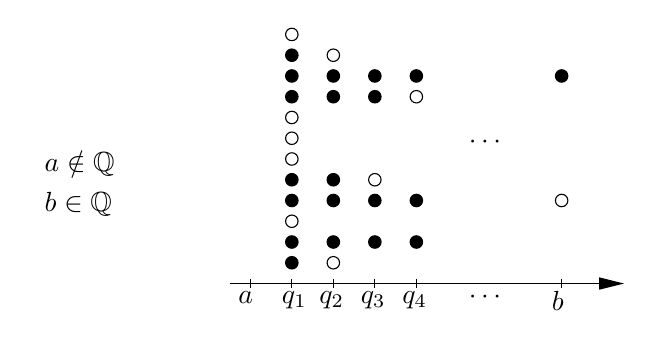
\begin{tikzpicture}[x=0.75pt,y=0.75pt,yscale=-1,xscale=1]
		%uncomment if require: \path (0,300); %set diagram left start at 0, and has height of 300

		\draw    (130,180) -- (318,180) ;
		\draw [shift={(320,180)}, rotate = 180] [fill={rgb, 255:red, 0; green, 0; blue, 0 }  ][line width=0.08]  [draw opacity=0] (12,-3) -- (0,0) -- (12,3) -- cycle    ;
		\draw  [fill={rgb, 255:red, 0; green, 0; blue, 0 }  ,fill opacity=1 ] (157,170) .. controls (157,168.34) and (158.34,167) .. (160,167) .. controls (161.66,167) and (163,168.34) .. (163,170) .. controls (163,171.66) and (161.66,173) .. (160,173) .. controls (158.34,173) and (157,171.66) .. (157,170) -- cycle ;
		\draw  [fill={rgb, 255:red, 0; green, 0; blue, 0 }  ,fill opacity=1 ] (157,160) .. controls (157,158.34) and (158.34,157) .. (160,157) .. controls (161.66,157) and (163,158.34) .. (163,160) .. controls (163,161.66) and (161.66,163) .. (160,163) .. controls (158.34,163) and (157,161.66) .. (157,160) -- cycle ;
		\draw   (157,150) .. controls (157,148.34) and (158.34,147) .. (160,147) .. controls (161.66,147) and (163,148.34) .. (163,150) .. controls (163,151.66) and (161.66,153) .. (160,153) .. controls (158.34,153) and (157,151.66) .. (157,150) -- cycle ;
		\draw  [fill={rgb, 255:red, 0; green, 0; blue, 0 }  ,fill opacity=1 ] (157,140) .. controls (157,138.34) and (158.34,137) .. (160,137) .. controls (161.66,137) and (163,138.34) .. (163,140) .. controls (163,141.66) and (161.66,143) .. (160,143) .. controls (158.34,143) and (157,141.66) .. (157,140) -- cycle ;
		\draw  [fill={rgb, 255:red, 0; green, 0; blue, 0 }  ,fill opacity=1 ] (157,130) .. controls (157,128.34) and (158.34,127) .. (160,127) .. controls (161.66,127) and (163,128.34) .. (163,130) .. controls (163,131.66) and (161.66,133) .. (160,133) .. controls (158.34,133) and (157,131.66) .. (157,130) -- cycle ;
		\draw   (157,120) .. controls (157,118.34) and (158.34,117) .. (160,117) .. controls (161.66,117) and (163,118.34) .. (163,120) .. controls (163,121.66) and (161.66,123) .. (160,123) .. controls (158.34,123) and (157,121.66) .. (157,120) -- cycle ;
		\draw   (157,110) .. controls (157,108.34) and (158.34,107) .. (160,107) .. controls (161.66,107) and (163,108.34) .. (163,110) .. controls (163,111.66) and (161.66,113) .. (160,113) .. controls (158.34,113) and (157,111.66) .. (157,110) -- cycle ;
		\draw   (157,100) .. controls (157,98.34) and (158.34,97) .. (160,97) .. controls (161.66,97) and (163,98.34) .. (163,100) .. controls (163,101.66) and (161.66,103) .. (160,103) .. controls (158.34,103) and (157,101.66) .. (157,100) -- cycle ;
		\draw  [fill={rgb, 255:red, 0; green, 0; blue, 0 }  ,fill opacity=1 ] (157,90) .. controls (157,88.34) and (158.34,87) .. (160,87) .. controls (161.66,87) and (163,88.34) .. (163,90) .. controls (163,91.66) and (161.66,93) .. (160,93) .. controls (158.34,93) and (157,91.66) .. (157,90) -- cycle ;
		\draw  [fill={rgb, 255:red, 0; green, 0; blue, 0 }  ,fill opacity=1 ] (157,80) .. controls (157,78.34) and (158.34,77) .. (160,77) .. controls (161.66,77) and (163,78.34) .. (163,80) .. controls (163,81.66) and (161.66,83) .. (160,83) .. controls (158.34,83) and (157,81.66) .. (157,80) -- cycle ;
		\draw  [fill={rgb, 255:red, 0; green, 0; blue, 0 }  ,fill opacity=1 ] (157,70) .. controls (157,68.34) and (158.34,67) .. (160,67) .. controls (161.66,67) and (163,68.34) .. (163,70) .. controls (163,71.66) and (161.66,73) .. (160,73) .. controls (158.34,73) and (157,71.66) .. (157,70) -- cycle ;
		\draw   (157,60) .. controls (157,58.34) and (158.34,57) .. (160,57) .. controls (161.66,57) and (163,58.34) .. (163,60) .. controls (163,61.66) and (161.66,63) .. (160,63) .. controls (158.34,63) and (157,61.66) .. (157,60) -- cycle ;
		\draw   (177,170) .. controls (177,168.34) and (178.34,167) .. (180,167) .. controls (181.66,167) and (183,168.34) .. (183,170) .. controls (183,171.66) and (181.66,173) .. (180,173) .. controls (178.34,173) and (177,171.66) .. (177,170) -- cycle ;
		\draw  [fill={rgb, 255:red, 0; green, 0; blue, 0 }  ,fill opacity=1 ] (177,160) .. controls (177,158.34) and (178.34,157) .. (180,157) .. controls (181.66,157) and (183,158.34) .. (183,160) .. controls (183,161.66) and (181.66,163) .. (180,163) .. controls (178.34,163) and (177,161.66) .. (177,160) -- cycle ;
		\draw  [fill={rgb, 255:red, 0; green, 0; blue, 0 }  ,fill opacity=1 ] (177,140) .. controls (177,138.34) and (178.34,137) .. (180,137) .. controls (181.66,137) and (183,138.34) .. (183,140) .. controls (183,141.66) and (181.66,143) .. (180,143) .. controls (178.34,143) and (177,141.66) .. (177,140) -- cycle ;
		\draw  [fill={rgb, 255:red, 0; green, 0; blue, 0 }  ,fill opacity=1 ] (177,130) .. controls (177,128.34) and (178.34,127) .. (180,127) .. controls (181.66,127) and (183,128.34) .. (183,130) .. controls (183,131.66) and (181.66,133) .. (180,133) .. controls (178.34,133) and (177,131.66) .. (177,130) -- cycle ;
		\draw  [fill={rgb, 255:red, 0; green, 0; blue, 0 }  ,fill opacity=1 ] (177,90) .. controls (177,88.34) and (178.34,87) .. (180,87) .. controls (181.66,87) and (183,88.34) .. (183,90) .. controls (183,91.66) and (181.66,93) .. (180,93) .. controls (178.34,93) and (177,91.66) .. (177,90) -- cycle ;
		\draw  [fill={rgb, 255:red, 0; green, 0; blue, 0 }  ,fill opacity=1 ] (177,80) .. controls (177,78.34) and (178.34,77) .. (180,77) .. controls (181.66,77) and (183,78.34) .. (183,80) .. controls (183,81.66) and (181.66,83) .. (180,83) .. controls (178.34,83) and (177,81.66) .. (177,80) -- cycle ;
		\draw   (177,70) .. controls (177,68.34) and (178.34,67) .. (180,67) .. controls (181.66,67) and (183,68.34) .. (183,70) .. controls (183,71.66) and (181.66,73) .. (180,73) .. controls (178.34,73) and (177,71.66) .. (177,70) -- cycle ;
		\draw  [fill={rgb, 255:red, 0; green, 0; blue, 0 }  ,fill opacity=1 ] (197,160) .. controls (197,158.34) and (198.34,157) .. (200,157) .. controls (201.66,157) and (203,158.34) .. (203,160) .. controls (203,161.66) and (201.66,163) .. (200,163) .. controls (198.34,163) and (197,161.66) .. (197,160) -- cycle ;
		\draw  [fill={rgb, 255:red, 0; green, 0; blue, 0 }  ,fill opacity=1 ] (197,140) .. controls (197,138.34) and (198.34,137) .. (200,137) .. controls (201.66,137) and (203,138.34) .. (203,140) .. controls (203,141.66) and (201.66,143) .. (200,143) .. controls (198.34,143) and (197,141.66) .. (197,140) -- cycle ;
		\draw   (197,130) .. controls (197,128.34) and (198.34,127) .. (200,127) .. controls (201.66,127) and (203,128.34) .. (203,130) .. controls (203,131.66) and (201.66,133) .. (200,133) .. controls (198.34,133) and (197,131.66) .. (197,130) -- cycle ;
		\draw  [fill={rgb, 255:red, 0; green, 0; blue, 0 }  ,fill opacity=1 ] (197,80) .. controls (197,78.34) and (198.34,77) .. (200,77) .. controls (201.66,77) and (203,78.34) .. (203,80) .. controls (203,81.66) and (201.66,83) .. (200,83) .. controls (198.34,83) and (197,81.66) .. (197,80) -- cycle ;
		\draw  [fill={rgb, 255:red, 0; green, 0; blue, 0 }  ,fill opacity=1 ] (217,160) .. controls (217,158.34) and (218.34,157) .. (220,157) .. controls (221.66,157) and (223,158.34) .. (223,160) .. controls (223,161.66) and (221.66,163) .. (220,163) .. controls (218.34,163) and (217,161.66) .. (217,160) -- cycle ;
		\draw   (217,90) .. controls (217,88.34) and (218.34,87) .. (220,87) .. controls (221.66,87) and (223,88.34) .. (223,90) .. controls (223,91.66) and (221.66,93) .. (220,93) .. controls (218.34,93) and (217,91.66) .. (217,90) -- cycle ;
		\draw  [fill={rgb, 255:red, 0; green, 0; blue, 0 }  ,fill opacity=1 ] (217,80) .. controls (217,78.34) and (218.34,77) .. (220,77) .. controls (221.66,77) and (223,78.34) .. (223,80) .. controls (223,81.66) and (221.66,83) .. (220,83) .. controls (218.34,83) and (217,81.66) .. (217,80) -- cycle ;
		\draw    (160,178) -- (160,182) ;
		\draw    (180,178) -- (180,182) ;
		\draw    (200,178) -- (200,182) ;
		\draw    (220,178) -- (220,182) ;
		\draw    (140,178) -- (140,182) ;
		\draw    (290,178) -- (290,182) ;
		\draw   (287,140) .. controls (287,138.34) and (288.34,137) .. (290,137) .. controls (291.66,137) and (293,138.34) .. (293,140) .. controls (293,141.66) and (291.66,143) .. (290,143) .. controls (288.34,143) and (287,141.66) .. (287,140) -- cycle ;
		\draw  [fill={rgb, 255:red, 0; green, 0; blue, 0 }  ,fill opacity=1 ] (287,80) .. controls (287,78.34) and (288.34,77) .. (290,77) .. controls (291.66,77) and (293,78.34) .. (293,80) .. controls (293,81.66) and (291.66,83) .. (290,83) .. controls (288.34,83) and (287,81.66) .. (287,80) -- cycle ;
		\draw  [fill={rgb, 255:red, 0; green, 0; blue, 0 }  ,fill opacity=1 ] (197,90) .. controls (197,88.34) and (198.34,87) .. (200,87) .. controls (201.66,87) and (203,88.34) .. (203,90) .. controls (203,91.66) and (201.66,93) .. (200,93) .. controls (198.34,93) and (197,91.66) .. (197,90) -- cycle ;
		\draw  [fill={rgb, 255:red, 0; green, 0; blue, 0 }  ,fill opacity=1 ] (217,140) .. controls (217,138.34) and (218.34,137) .. (220,137) .. controls (221.66,137) and (223,138.34) .. (223,140) .. controls (223,141.66) and (221.66,143) .. (220,143) .. controls (218.34,143) and (217,141.66) .. (217,140) -- cycle ;

		\draw (154,182.4) node [anchor=north west][inner sep=0.75pt]    {$q_{1}$};
		\draw (284,182.4) node [anchor=north west][inner sep=0.75pt]    {$b$};
		\draw (172,182.4) node [anchor=north west][inner sep=0.75pt]    {$q_{2}$};
		\draw (192,182.4) node [anchor=north west][inner sep=0.75pt]    {$q_{3}$};
		\draw (212,182.4) node [anchor=north west][inner sep=0.75pt]    {$q_{4}$};
		\draw (244,182.4) node [anchor=north west][inner sep=0.75pt]    {$\cdots $};
		\draw (133,182.4) node [anchor=north west][inner sep=0.75pt]    {$a$};
		\draw (244,107.9) node [anchor=north west][inner sep=0.75pt]    {$\cdots $};
		\draw (33,111.4) node [anchor=north west][inner sep=0.75pt]    {$ \begin{array}{l}
		a\notin \QQ\\
		b\in \QQ
		\end{array}$};
		\end{tikzpicture}
	\end{figure}
	\FloatBarrier
	
	\textit{Step 2}: Then fix $\eps > 0$. Via equicontinuity, we find $\delta=\delta(\eps)>0$ such that: $$|f_{n_h}(t_1)-f_{n_h}(t_2)|<\tfrac{\eps}{3} \quad \forall t_1,t_2 \in [a,b] :|t_1-t_2|<\delta \quad \forall h \in \NN.$$
	
	Consider now a family of intervals $I_i=\{[a_j, b_j]\}^N_{j=1}$ such that $b_j-a_j < \delta$ and $\cup_{j=1}^N [a_j,b_j]=[a,b]$. Then, for any $i$, we can choose $q_i \in I_i$, because $\QQ$ is dense in $\RR$.
	
	Observe that there exists $h_0(\eps) \in \NN$, independent of $j$, such that\footnote{Since this can be done for any $j$, it's enough to take the biggest, as $N$ is finite.}:
	$$|f_{n_h}(q_j)-f_{n_{h'}}(q_j)|\leq \tfrac{\eps}{3} \quad \forall h,h' > h_0 \quad \forall j = 1, \ldots, N.$$
	
	\textit{Step 3}: Let $t\in[a,b]$. Then $t \in I_i$ for some $i \in 1:N$, thus $|t-q_i|<\delta$. Therefore we have, for any $h, h'>h_0$:
	\begin{align*}
	|f_{n_h}(t)-f_{n_{h'}}(t)|
	&\leq |f_{n_h}(t)-f_{n_h}(q_j)|+|f_{n_h}(q_j)-f_{n_{h'}}(q_j)|+|f_{n_{h'}}(q_j)-f_{n_{h'}}(t)| \\
	&\le \tfrac{\eps}{3}+\tfrac{\eps}{3}+\tfrac{\eps}{3}\\
	&= \eps
	\end{align*}
	
	Thus $\{f_{n_h}\}$ is a uniform Cauchy sequence, that is a Cauchy sequence with respect to $\norm{\cdot}_\infty$, and it converges in the Banach space $(\Cc([a,b]),\norm{\cdot}_\infty)$.
\end{proof}


Also it can be shown that the boundedness and equicontinuity are also necessary for compactness in $(\Cc([a,b]), \norm{\cdot}_\infty)$.

Actually, equicontinuity and equiboundedness are also necessary conditions: namely, if $K \subset \Cc([a,b])$ is compact, then any $\{f_n\}\subset K$ satisfies them.

How this theorem is related to compactness? Apparently in the theorem formulation there is no mention to compactness but we see in the following example that exists a strong relation.

\begin{exam}
	Consider the following subset of $(\Cc([a,b]), \norm{\cdot}_\infty)$: 
	$$ 
	E_M 
	= \{
	f \in \Cc^1([a,b]) :\ 
	\norm{f}_\infty + \norm{f'}_\infty \leq M
	\}
	$$
	for some given $M > 0$.
	
	Thanks to the Ascoli--Arzelà theorem, we can prove that $E_M$ is sequentially compact, and so it is also compact. Indeed, take a sequence $\{f_n\}_{n\in \NN} \subset E_M$: it is bounded and, owing to the Lagrange theorem, we have: 
	$$
	\abs{f_n(x) - f_n(y)} 
	\leq M \abs{x-y} 
	\quad \forall x,y \in [a,b], \ 
	\forall n \in \NN
	.
	$$
	Thus the sequence is also equicontinuous so it contains a subsequence which converges uniformly to some $f \in E_M$.
\end{exam}






%!TEX root = ../main.tex
\subsubsection{\texorpdfstring{$L^p$}{Lp} spaces} \label{chapter-Lp-spaces}
As we have seen in Banach spaces examples, we are interested in investigating whether functional spaces are Banach. Our goal in this section is to prove that the spaces related to Lebesgue-integrable functions are Banach. First recall the definition of the space of Lebesgue-integral function $\Lc^1$  (see definition \vref{space-lebesgue-integrable-functions}) and the definition of the space $L^1$ (see definition \vref{L1-space}). Here we define many other spaces related to those; a relevant fact is that all these spaces have a vector space structure.

\begin{defn}
	Let $(\Omega,\mm,\mu)$ be complete measure space and fix $p \in [1,\infty)$.
	$$
	\Lc^p(\Omega, \mm, \mu) 
	\coloneqq\{
		f:\Omega \to \RR \text{ measurable} :
		\enspace |f|^p \in \Lc^1(\Omega, \mm,\mu)
		\}
	;
	$$
	or, equivalently:
	$$\Lc^p(\Omega, \mm, \mu) \coloneqq\{f:\Omega \to \RR \text{ measurable} : \enspace \int_\Omega |f|^p \dmu < \infty\}.$$
	
	In addition, we define:
	$$
	L^p(\Omega,\mm,\mu)
	\coloneqq\frac{\Lc^p(\Omega,\mm, \mu)}{\sim}
	$$
	where the equivalence relation is $f \sim g \iff f=g$ almost everywhere with respect to  $\mu$ in $\Omega$. 
\end{defn}

Since the inequality 
$$
\left(\frac{x+y}{2} \right)^p 
\leq \frac 1 2 |x|^p + \frac 1 2 |y| ^ p 
\quad \forall	\, x,y 
\geq 0
$$
holds, then $L^p(\Omega,\mm,\mu)$ is a vector space on $\RR$ with respect to the standard operations: $\{f\}+\{g\}$, $\alpha\{f\}$.

For each of those spaces we can define its associated norm.
\begin{defn}
	Let $p\in[1, +\infty)$. \\
	Then 
	$$
	\norm{f}_p 
	\coloneqq\left(\int_\Omega |f|^p \dmu \right)^{\frac 1 p}
	$$ 
	is a norm in $L^p(\Omega, \mm, \mu)$.
\end{defn}
The reader should check this definition satisfy all the property required to a norm, except for the triangular inequality property which coincides with the Minkowsky's theorem (see \vref{prop-mink-ineq}), which will be presented here.

\begin{defn}
	We define:
	$$
		\Lc^\infty(\Omega, \mm, \mu) 
		\coloneqq\{f:\Omega \to \RR \text{ measurable} : \enspace \esssup f < +\infty\}
	;
	$$
	and with the same equivalence relation of the previous definition we set:
	$$
		L^\infty(\Omega,\mm,\mu) 
		\coloneqq\frac{\Lc^\infty(\Omega,\mm, \mu)}{\sim}
	.
	$$
\end{defn}

Notice that also $L^\infty$ is a vector space on $\RR$. 

\begin{defn}
	The following
	$$
		\norm{f}_\infty
		\coloneqq \esssup_\Omega \left(|f|\right)
	$$ 
	is a norm in $L^\infty(\Omega, \mm, \mu)$.
\end{defn}

Then we have for $p \in [1, \infty]$ that $(L^p(\Omega, \mm, \mu), \norm{\cdot}_p)$ are normed vector spaces.
Notice that $L^p$ with those norms are not normed vector spaces as $\norm{f}=0$ implies that $f=0$ except for a null measure set, while the definition requires that this holds anywhere in $\Omega$.

From those norm it's easy to obtain a notion of metric for each $p$, called $d_p$. We have already introduced those in the chapter about topology (\vref{topology-section}). With $L^p$ spaces, those distances defines metric spaces. However, $\Lc^p$ aren't a metric spaces with respect to $d_p$ as $d_p(f,g) = 0$ implies only that $f=g$ a.e.\ in $\Omega$.


\paragraph{Relevant inequalities} Here are presented three well-known inequalities which are extremely useful for the development of the theory. In order to make the steps more clear, here we do not used the norm notation, but we added this convention at the end of each proposition.

\begin{defn}
	Let $p\in(1, +\infty)$.\\
	The number $q \in (1, +\infty)$ is called the \emph{conjugate} of $p$ if 
	$$\tfrac 1 p + \tfrac 1 q = 1.$$
	By extension, the conjugate of $p=1$ is $q=\infty$ and of $p=\infty$ is $q=1$.
\end{defn}

Sometimes the conjugate of $p$ is written as $p^\star$.

\begin{prop}[Young's inequality] \label{young-ineq}
	For all $a,b > 0$ we have:
	$$ab\leq \frac{a^p}{p} + \frac{b^q}{q},$$
	where $p \in (1, \infty)$ and $q$ is its conjugate index.
\end{prop}
\begin{proof}
	Fix $b>0$ and take $\phi(a) \coloneqq \frac{a^p}{p} + \frac{b^q}{q} - ab$ on $(0,\infty)$.\\
	Proof follows from the fact that $\phi$ is convex with a positive absolute minimum.
\end{proof}

\begin{prop}[Hölder's inequality]
	Consider two function $f\in L^p(\Omega,\mm,\mu)$, $g \in L^q(\Omega,\mm\,\mu)$, with $p \in (1, \infty)$ and $q$ its conjugate index.\\	
	Then $f,g \in L^1(\Omega,\mm,\mu)$, and:
	$$
	\int_\Omega |fg|\,\dmu 
	\leq 	\left( \int_\Omega |f|^p \, \dmu \right )^{1/p}
			\left( \int_\Omega |g|^q \, \dmu \right )^{1/q}
	.
	$$
	In terms of norms, this equality can be written as:
	$$
	\norm{fg}_1
	\leq \norm{f}_p \cdot \norm{g}_q
	.
	$$
\end{prop}
\begin{proof}
		Suppose $p\in(1, +\infty)$ and $f$, $g > 0$ a.e. Consider:
		$$F(t)=\frac{f(t)}{(\int_\Omega|f(t)|^p \,\dmu)^{1/p}}
		\quad \text{and} \quad
		G(t)=\frac{g(t)}{(\int_\Omega|g(t)|^q \,\dmu)^{1/q}}$$
		
		Using Young's inequality (\vref{young-ineq}), we get:
		\begin{align*}
			|FG| &\leq \tfrac 1 p |F|^p + \tfrac 1 q |G|^q \\
		   	\int_\Omega|FG| \,\dmu &\leq \tfrac 1 p \int_\Omega|F|^p \,\dmu + \tfrac 1 q \int_\Omega|G|^q \,\dmu \\
			&\leq \tfrac 1 p \int_\Omega \abs{\frac{f(t)}{(\int_\Omega|f(t)|^p\,\dmu)^{1/p}}}^p \,\dmu + \tfrac 1 q \int_\Omega \abs{\frac{g(t)}{(\int_\Omega|g(t)|^q\,\dmu)^{1/q}}}^q \,\dmu \\
			&= \tfrac 1 p + \tfrac 1 q = 1 \\
			\int_\Omega |fg| \,\dmu &\leq \left(\int_\Omega |f|^p \,\dmu\right)^{1/p}\left( \int_\Omega |g|^q\right)^{1/q}
		\end{align*}
		
		When $p=1, q=\infty$, the proof is trivial:
		$$\int_\Omega|fg|\leq \int_\Omega |f| \esssup\limits_\Omega |g| \dmu = \esssup\limits_\Omega |g| \int_\Omega |f| \dmu$$
		
		When $p= +\infty$:
		$$\int_\Omega|fg| \dmu \leq \esssup\limits_\Omega |f| \int_\Omega |g| \dmu$$
\end{proof}

Another proof consist of considering: $$\norm{fg} = \int_\Omega \frac{\norm{g}_q^{\frac 1 p}}{\norm{f}_p^{\frac 1 q}} f \cdot \frac{\norm{f}_p^{\frac 1 q}}{\norm{g}_q^{\frac 1 p}} g,$$ apply the young inequality and operate the proper calculations. 

\begin{prop}[Minkowsky's inequality]\label{prop-mink-ineq}
	Let $f, g \in L^p(\Omega,\mm,\mu)$ and $p \in (1, \infty)$.\\
	Then:
	$$\left(\int_\Omega |f+g|^p \dmu \right)^{\frac 1 p} \leq \left(\int_\Omega |f|^p \dmu\right)^{\frac 1 p}+\left(\int_\Omega |g|^p \dmu\right)^{\frac 1 p}.$$
	In terms of norms, this equality can be written as:
	$$
	\norm{f+g}_p
	\leq \norm{f}_p + \norm{g}_p
	$$
\end{prop}

Observe that this result shows the triangular inequality for the $p$ norms.

\begin{proof}
	The prove in case of $p=1$ is trivial, here the general case:
	\begin{align*}
		\int_\Omega |f+g|^p \dmu &= \int_\Omega |f+g| |f+g|^{p-1} \dmu \\
		&\leq \int_\Omega |f||f+g|^{p-1}\dmu + \int_\Omega |g||f+g|^{p-1} \dmu \\
		& \leq \left(\int_\Omega |f|^p \dmu\right)^{\frac 1 p}
		\left(\int_\Omega|f+g|^p \dmu\right)^{\frac{p-1}{p}} \\
		&\qquad + \left(\int_\Omega |g|^p \dmu\right)^{\frac 1 p}\left(\int_\Omega|f+g|^p\dmu\right)^{\frac{p-1}{p}} \\
		& = \left[\left(\int_\Omega |f|^p \dmu\right)^{\frac 1 p}+\left(\int_\Omega |g|^p \dmu\right)^{\frac 1 p}\right] \left( \int_\Omega |f+g| ^p \dmu\right)^{\frac{p-1}{p}}.
	\end{align*}
	As $f+g \in L^p(\Omega, \mm, \mu)$ the thesis follows.
\end{proof}

\paragraph{Relationship between $L^p$ spaces} Now we try to understand how those spaces are related and some of their properties. The $L^p$ spaces, if $\mu$ is finite, make up an ascending chain (see definition \vref{chain-defn}) with respect to the inclusion. The greater is $p$, the less functions belongs. Indeed we have the following result:
\begin{prop}\label{prop-relations-between-Lp}
	If $\mu(\Omega) < +\infty$ and $1 \leq s \leq r \leq \infty$, we have:
	$$L^r(\Omega,\mm,\mu)\subseteq L^s(\Omega,\mm,\mu)$$
	and the norm can be controlled:
	$$\norm{f}_s \leq \left(\mu(\Omega)\right)^{\frac 1 s - \frac 1 r}\norm{f}_r.$$
\end{prop}
\begin{proof}
	Suppose $r\leq \infty$ and take $f\in L^r(\Omega, \mm, \mu)$ and apply the Hölder's inequality with $q = \frac r s$ and $p = \frac{r}{r-s}$:
	$$
	\norm{f}_s^s
	=\int_\Omega |f|^s \dmu 
	= \int_\Omega 1 \cdot |f|^s 
	\leq 
		\left(\int_\Omega \dmu\right)^{\left(\frac{r-s}{r} \right)}
		\left(\int_\Omega |f|^{s \cdot \frac r s} \dmu\right)^{\frac s r }
	= \mu(\Omega)^{\left(\frac{r-s}{r} \right)}\norm{f}_r^s
	$$
	where and the thesis follows.
	In case of $r=\infty$, we could repeat the same argument, but there is a simpler way:
	$$
	\int_\Omega |f|^s \dmu 
	\leq \int_\Omega \esssup_\Omega (|f|^s) \dmu 
	\leq \int_\Omega (\esssup_\Omega |f|)^s \dmu 
	= \mu(\Omega)\norm{f}^s_\infty
	.
	$$
\end{proof}
In such case, $L^1$ contains all functions that belong to $L^p$ for any $p$.

However, if $\mu(\Omega)=\infty$, then the former inclusion does not hold in general, consider the following example.
\begin{exam}
	Consider $(\RR, \Lc(\RR), \lambda)$ and let:
	$$f_\alpha(x) \coloneqq \frac{1}{x^\alpha}\Ind_{[1,\infty]} \quad \text{with } \alpha \in (0,1).$$
	So $f_\alpha \in L^r$ for any $r > \alpha^{-1}$, but $f_\alpha \notin L^s$ for any $s \in [1, \alpha^{-1}].$
\end{exam}

\paragraph{The $l^p$ spaces}  The chain of inclusions can be descending in a very special case. Indeed, we can define 
$$
l^p
\coloneqq L^p(\NN,\Pc(\NN),\mu_c)
$$
and the following proposition holds:
\begin{prop}
	For $1 \leq s \leq r \leq \infty$ we have:
	$$ l^s \subseteq l^r, \qquad \norm{f}_r \leq \norm{f}_s.$$
	The inclusion is strict if $s \neq r$.
\end{prop}
\begin{proof}
	We recall that $l^p$ spaces are correspondent to $L^p(\NN ,\Pc(\NN) ,\mu_c)$, with the counting measure.

	\textit{Step 1}: Let us prove that $l^p \varsubsetneq l^{\infty}$ for any $p\in [ 1,+\infty )$.

	Consider $x\in l^p$, then\footnote{This very first point is what can't be done in $L^p$ spaces, namely if $f\in L^p$ then not necessarily $f(x)\to 0$ as $x\to \infty $. Indeed take $p=1$ and consider $f(x) =\Ind_{\{n,n+1/n^2\}}(x)$ where $n\in \NN$. You can easily check that its $L^1$ norm converges $(\sum _{n\in \NN} 1/n^2 < +\infty)$, however its limit as $x\to \infty $ is not $0$.}
	$$
		\sum\limits _{n\in \NN}| x_n| ^{p} < +\infty \implies  | x_n| \to 0 \ \text{as} \ n\to  +\infty 
	$$
	In particular, $\{x_n\}_{n\in \NN}$ is bounded, so that $\sup _{n\in \NN}| x_n| < +\infty $, hence $x\in l^{\infty}$. Moreover $l^p \neq l^{\infty}$, indeed consider the sequence $x=\{x_n\}_{n\in \NN}$ defined as $x_n =1$ for any $n\in \NN$, which belongs to $l^{\infty}$ (its norm is $1$) but not to $l^p$, since $\sum _{n\in \NN} 1^{p}$ diverges.

	\textit{Step 2}: Let us prove that $l^r \subset l^s$ for any $1\leq r< s< +\infty $.

	Consider $x\in l^r$, we can assume $x\neq 0$ (the sequence with all zeros). Define now
	$$
		y=\{y_{n}\}_{n\in \NN} ,\ \ y_{n} =\frac{x_n}{\norm{x}_r} .
	$$
	Observe that $y\in l^r$, indeed $l^r$ is a vector space, and
	$$
		\norm{y}_r = \norm{\frac{x}{\norm{x}_r}}_r =\frac{1}{\norm{x}_r}\norm{x}_r =1
	$$
	This implies that
	$$
		|y_{n}| \leq 1,\ \forall n\in \NN \ \ \implies  \ \ | y_{n}| ^{s} \leq | y_{n}| ^{r} \ \ \implies  \ \ \sum\limits _{n\in \NN}| y_{n}| ^{s} \leq \sum\limits _{n\in \NN}| y_{n}| ^{r} < +\infty ,
	$$
	hence $y\in l^s$ and $x=y\cdot \norm{x}_r \in l^s$ (also $l^s$ is a vector space).

	Moreover, $l^r \neq l^s$, indeed consider
	$$
		x=\{x_n\}_{n\in \NN} ,\ \ x_n =\frac{1}{n^{1/r}}
	$$
	then
	\begin{align*}
		\sum\limits _{n\in \NN}| x_n| ^{r} &=\sum\limits _{n\in \NN}\frac{1}{n} \ =+\infty \ \ \implies  \ \ x\notin l^r\\
		\sum\limits _{n\in \NN}| x_n| ^{s} &=\sum\limits _{n\in \NN}\frac{1}{n^{s/r}} < +\infty \ \ \implies  \ \ x\in l^s
	\end{align*}
\end{proof}


Remember that a function defined on $\NN$ can be seen as a sequence.

\paragraph{$L^p$ spaces are Banach spaces} The following is a very relevant result.

\begin{theo}\label{Lp-norm-banach}
	$(L^p(\Omega,\mm,\mu), \norm{\cdot}_p)$ is a Banach space for any $p \in [1, +\infty]$.
\end{theo}

\begin{proof} \textit{Case $p \in [1, +\infty)$}:\\
	We are going to use the characterization of Banach spaces through the convergence of series (see theorem \vref{theo-banach-space-charact}): a series converges only if converges the series of absolute values.
	
	\textit{Step 0}: Let $\{f_n\}_{n \in \NN} \subset L^p$ be such that $\sum_{n\in\NN} \norm{f_n}_p<+\infty$.\\
	We need to prove that $\sum_{n\in\NN} f_n$ converges in $L^p(\Omega,\mm,\mu)$, from the characterization we have the thesis.
	
	\textit{Step 1, convergence in $\Omega$}: Set $g_h(t) = \sum_{n=0}^{h}|f_n(t)|$; from Minkowsky's inequality we have that $g_h \in L^p$  (see proposition \vref{prop-mink-ineq}):
	$$
		\norm{g_h}_{L^p} 
		\leq \sum_{n=0}^h \norm{f_n}_p
		\leq \sum_{n\in \NN} \norm{f_n}_p 
		< + \infty \quad
		\forall h \in \NN
	.
	$$
	
	Since $g_h$ is an increasing sequence, by monotone convergence (see theorem \vref{monotone-convergence}) we have:
	$$
		\lim_{h \to +\infty} \int_\Omega |g_h(t)|^p \,\dmu
		= \int_\Omega \lim_{h \to +\infty} |g_h(t)|^p \,\dmu
		= \int_\Omega g (t)^p \,\dmu
	$$ 
	where $g(t) = \lim_{h \to +\infty}g_h(t)$ and, as its norm is bounded, $g \in L^p$ (the absolute value can be removed as $g$ is positive by definition).\\
	Thus $|g(t)| < +\infty$ for almost any $t$ in $\Omega$.
	
	Therefore we have 
	$$
		\sum_{n\in \NN} f_n(t) 
		< +\infty
		\quad \text{for almost any } t
	,
	$$ 
	the series converges almost everywhere in $\Omega$.
	
	\textit{Step 2, convergence in $L^p$}: Set now:
	$$
		S(t)
		=\sum_{n\in \NN} f_n(t) 
		\text{ and } 
		S_h(t)
		=\sum_{n=0}^{h} f_n(t)
	.
	$$
	For almost any $t \in \Omega$, using the triangular inequality, we have:
	$$
		|S(t) - S_h(t)|^p 
		= \abs{\sum_{n = h+1}^{+\infty} f_n(t)}^p
		\leq \left( \sum_{n \in \NN} |f_n(t)| \right)^p
		= (g(t))^p \in L^1
	.
	$$
	Then, using dominated convergence (see theorem \vref{dominated-convergence}), we have 
	$\norm{S-S_h}_p \to 0 \text{ as } h\to +\infty$, that is $\sum_{n\in\NN} f_n$ converges in $L^p$.
	
	By the characterization theorem, the proof of the considered case is complete.
	
	\textit{Case $p = \infty$, step 1}:\\
	Let $\{f_n\}_{n\in\NN}\subset L^\infty(\Omega,\mm,\mu)$ be a Cauchy sequence, and take those two sets:
	\begin{align*}
		A_n 
		&= \{
			t\in \Omega : 
			\ |f_n(t)|>\norm{f_n}_\infty
		\} \\
		B_{m,n} 
		&= \{
			t\in \Omega : 
			\ |f_n(t)-f_m(t)|>\norm{f_n-f_m}_\infty
		\}
	\end{align*}
	where the inequalities are given by definition of the essential supremum. Notice that we defined those two sequences of sets which catch discontinuity points in the domain, for each $f_n$.\\
	We have
	$$
		\mu(A_n) 
		= \mu(B_{m,n})
		= 0
		\quad \forall m,n 
		\in \NN
	, 
		\quad \text{and}
		\quad E 
		= \left(\bigcup_{n \in \NN} A_n \right)
		\cup \left(\bigcup_{m,n\in \NN}B_{m,n}\right)
	$$
	has zero measure.
	
	Then, for all $t \in E\comp$, we have that the sequence $\{f_n(t)\}_{n\in\NN}$ converges to some measurable $f$. Moreover $f \in L^\infty(\Omega,\mm,\mu)$ since $\{f_n(t)\}_{n\in\NN}$ is bounded in $L^\infty(\Omega,\mm,\mu)$, as it is a fundamental sequence.
	
	\textit{Step 2}: On the other hand, for any $\varepsilon > 0$ there is $n_0 = n_0(\varepsilon) \in \NN$ such that, for all $t \in E\comp$, we have:
	$$
		| f_n(t) - f_m(t) | 
		\leq \norm{f_n - f_m}_\infty < \varepsilon 
		\quad \forall m,n > n_0
	.
	$$
	As $m \to \infty$ we have:
	$$
		|f_n(t)-f|  
		\leq \varepsilon 
		\quad \forall n > n_0, 
		\quad \forall t \in E\comp
	$$
	from which we deduce that $\norm{f-f_n}_\infty \to 0$ as $n \to \infty$.\\
	And the proof is complete.
\end{proof}


\paragraph{The case $p \in (0,1)$} When $L^p$ spaces have $p$ less than $1$ things are not going straight. Those spaces does not have a vector space structure and is not possible to define a norm on them; but it is feasible to prove that $d_p(f,g)= \int_\Omega|f-g|^p \,\dmu$ is a metric and the corresponding $L^p(\Omega,\mm,\mu)$ is complete with respect to $d_p$.

However, the reverse Minkowsky's inequality holds:
$$
	\left(\int_\Omega(|f|+|g|)^p\dmu \right)^{\frac 1 p}
	\ge \left(\int_\Omega|f|^p\dmu\right)^{\frac 1 p}+\left(\int_\Omega|g|^p\dmu\right)^{\frac 1 p}
.
$$
Thus $\left(\int_\Omega |f|^p \dmu\right)^{\frac 1 p }$ is not a norm, because it does not respect the triangular inequality.
Anyway, inclusion chain follows the same rules as for $p>1$; if $\mu(\Omega)< \infty$ then we have:
$$
	L^r(\Omega, \mm, \mu) 
	\subseteq L^s(\Omega, \mm, \mu)
$$
for $0 < s \leq r \leq \infty$.
%!TEX root = ../main.tex
\subsubsection{Convergence and separability in \texorpdfstring{$L^p$}{Lp} spaces}


\paragraph{Convergence} Here some results on sequence of function convergence for those spaces.

\begin{prop}
	Let $p \in [1, +\infty)$, $\{f_n\} \subset L^p(\Omega,\mm,\mu)$ be a $L^p$-converging sequence.\\
	Then $\{f_n\}$ contains a subsequence which converges a.e. in $\Omega$.
\end{prop}

\begin{proof} The case $p = \infty$ is obvious while the case $p=1$ is already proved (see \vref{convergence-mean-implie-subsequence-ae}). Let's argue for the other cases.
	As $\{f_n\}_{n \in \NN} \to f$, we can apply the Chebyshev's inequality. Consider $\delta > 0$, we have:
	\begin{align*}
	\int_\Omega |f_n - f|^p \dmu
	&\geq \int _{\{t \in \Omega:\ |f_n - f | > \delta\}} |f_n(t) - f(t)|^p \dmu \\
	&\geq \delta^p \mu(\{t \in \Omega: \ |f_n - f| > \delta \}).
	\end{align*}
	This shows that $\{f_n\}_{n\in \NN}$ converges in measures, and the thesis follows (see theorem \vref{convergence-measure-implie-subsequence-ae}).
	%	Observe that $\{f_n\}_{n\in \NN}$ is a Cauchy sequence in $L^p$. Then we can construct a subsequence $\{f_{n_h}\}$ such that:
	%	$$\norm{f_{n_{h+1}}-f_{n_h}}_p\leq \frac{1}{h^2}$$
	%	Let $F_h \coloneqq f_{n_{h+1}}-f_{n_h}$. Therefore we have $\sum_{n \in \NN} \norm{F_h}_p < +\infty$.
	%	Then, arguing as in the proof of theorem \vref{theo-banach-space-charact}\todo{Check ref}, we deduce that $\sum_{h\in \NN_0} F_h$ converges a.e. to some $\tilde f \in L^p$. Then we have:
	%	\begin{align*}
	%	f_{n_{h+1}} &=f_{n_1}+\sum_{k=1}^h\left(f_{n_{h_{k+1}}}-f_{n_{h_k}} \right) \\
	%	f_{n_{h+1}} &\to f_{n_1}+\tilde f \in L^p \quad \text{a.e. in }\Omega
	%	\end{align*}
\end{proof}

Moreover we have the following result:

\begin{prop}
	Let $\{f_n\}\subset L^p(\Omega,\mm,\mu)$ with $p \in [1,\infty)$. \\
	If $f_n \to f$ in $L^p$ and $f_n \to g$ a.e. in $\Omega$, then $f=g \ a.e.$ in $\Omega$.
\end{prop}

\begin{proof}
	\begin{align*}
	\int_\Omega |f-g|^p \, \dmu
	&= \int_\Omega \lim\limits_{n\to+\infty}|f-f_n|^p \,\dmu\\ 
	&\leq \liminf_{n \to +\infty}\int_\Omega |f-f_n|^p \,\dmu & \text{(Fatou's lemma)}\\
	& = 0
	\end{align*}
	Thus $f=g$ a.e. in $\Omega$.
\end{proof}


\paragraph{A compactness criterion in $L^p$ spaces} Here we present a historically relevant result. First we introduce the notion of the shift operator.

\begin{defn}
	Given a function $f : \RR \to E$ and a shift value $h \in \RR$, the \emph{shift operator} is defined as follows:
	$$
	\tau_h f(x) 
	\coloneqq f(x+h)
	.
	$$
\end{defn}

The shift operator essentially evaluate the function after changing its argument, increasing or decreasing it.

\begin{theo}[Kolmogorov--Riesz--Frechét]\label{theo-KRF}
	Let $p\in [1, +\infty)$, and a bounded set $\Fc \subset L^p(\RR^N, \Lc(\RR^N),\lambda)$.\\
	If\footnote{This hypothesis can be equivalently formulated as follows: $\norm{\tau_h f - f} \to 0 \text{ as }\norm{h}_2 \to 0 \text{ uniformly in }\Fc$.} $\forall \eps > 0 \enspace \exists\, \delta = \delta (\eps) > 0$ such that:
	$$
	\norm{\tau_hf-f}_p < \eps \quad
	\forall f \in \Fc \quad
	\forall h \in \RR^N :\ \norm{h}_2 < \delta,
	$$
	for all $h\in\RR^N$ such that $|h| < \delta$ and any $f \in \Fc$, then $\Fc|_\Omega$ is precompact\footnote{A precompact set, also known as relatively compact subspace, is a subset whose closure is compact.} in $L^p(\RR^N, \Lc(\RR^N),\lambda)$ for any $\Omega \subset \RR^N$ of finite measure.
	
	Viceversa, if $E|_\Omega$ is precompact the above condition holds along with the \textit{tail condition}: for any $\eps > 0$ there exists $\Omega \subset \RR^N$ bounded and measurable such that $L^p$-norm of $f$ on $\Omega\comp$ is less then $\eps$ for all $f \in E$.
	%	$\forall \Omega \in \Lc(\Omega)$ such that $\lambda(\Omega)<+\infty$ we have that:\todo{Triple check}
	%	$$\overline{\Fc |_\Omega}^{\,L^p} = \overline{\left\{f|_\Omega : f \in \Fc \right\}}^{\,L^p} \text{ is compact in } L^p(\Omega, \Lc(\Omega), \lambda)$$
\end{theo}
%
%
%\begin{coro}
%	Let the hypotheses of the previous theorem hold.
%	If the following \emph{tail condition} also holds:
%	\begin{equation}
%	\forall \eps > 0 \quad \exists \, \Omega \in \Lc (\RR^N) \text{ bounded}:
%	\quad \norm{f}_{L^p(\RR^N \setminus \Omega)} <\eps \quad \forall f \in \Fc
%	\label{theo-rfk-tail-cond} \tag{$\star\star$}
%	\end{equation}
%	then $\widebar{\Fc}^{L^p}$ is compact in $L^p(\RR^N,\Lc(\RR^N),\lambda)$.
%	Moreover \eqref{theo-rfk-cond-1} and \eqref{theo-rfk-tail-cond} are also necessary.
%\end{coro}



\paragraph{Separability of $L^p(\RR)$} Here we discuss of $L^p$ spaces defined on $\RR$. Our goal now is to prove the following theorem (recall definition \vref{defn-separable-space}); to do that we need some other result.
\begin{theo}\label{Lp-separable}
	$L^p(\RR^N, \Lc(\RR^N), \lambda)$ is separable for all $p \in [1, +\infty)$.
\end{theo}
Observe that $p = \infty$ is excluded, we will face this case later. The proof will handle only the case $N = 1$. 

The pathway to prove this result will be the following.
\begin{enumerate}
\item[0.] $\Pc_{\QQ}([a,b])$ is dense in $\Cc([a,b])$ with the infinity norm (Stone--Weierstrass theorem).
\item Approximation of finite supported functions with $g\in \Cc_C(\RR)$ (Lusin theorem).
\item $\Sc(\RR)$ dense in $L^p(\RR)$ but not countable.
\item $\Cc_C(\RR)$ dense in $L^p(\RR)$ but not countable.
\item $\{P_m\Ind_{[-n,n]}\}$, the set of algebraic polynomials with restricted support, dense in $L^p(\RR)$ and countable.
\end{enumerate}

Meanwhile, notice the following, which is a weaker result highlighting the importance of topology:
\begin{prop}
	Let $\Omega \in \Lc(\RR)$ and take $E \coloneqq \{v \in L^p(\RR): v=0 \enspace \text{a.e. in }\Omega\comp\}$. \\
	Then $E$ is separable for any $p \in [1,\infty)$ with respect to the inherited topology, that is the topology on $E$ created by intersecting the open sets of $L^p(\RR)$ with $E$ itself.
\end{prop}
% (Indeed an open disc in $ \RR^3$ è chiuso perchè le sfere non entrano nel disco. se invece prendo l'intersezione delle sfere con il disco allora posso dire che è aperto)
% So it is important to specify the topology.


\paragraph{Continuous function with compact support} Let's build the tools that we will use for the proof.

\begin{defn}
	Let $g = \Omega \subseteq \RR \to \RR$ be continuous.\\
	The following set is called the \emph{support} of $g$:
	$$\supp(g) \coloneqq \overline{\{x \in \Omega: g(x) \neq 0\}}.$$
\end{defn}
In other words, the support is the subset of the domain of a function in which it has a value different from zero.

\begin{exam}
	Let: $$g(x) \coloneqq \begin{cases}
	e^{-\frac{1}{1-x^2}} & \text{if }|x| < 1 \\
	0 & \text{if }|x| \geq 1
	\end{cases}$$
	In this case $\supp(g) = [-1,1]$.
\end{exam}

Support is hence a set, and we know that there exist many kind of sets. In particular we are interested in the case of such set is compact.

\begin{defn}
	Let $\Omega \subseteq \RR$.
	$$
		\Cc_C(\Omega) 
		\coloneqq \{ f: \Omega \to \RR \text{ continuous with compact support} \}
	.
	$$
\end{defn}

We have define the set of continuous functions with compact support; the following result states that any Lebesgue measurable function can be approximated with one of those functions (similar to Stone--Weierstrass \vref{theo-stone-weierstrass}).

\begin{theo}[Lusin]\label{theo-lusin}
	Let $f:\RR\to \RR $ be Lebesgue measurable and let $\Omega \in \Lc(\RR)$ such that $\lambda (\Omega) < +\infty$. \\
	If $f(x)=0$ for any $\forall x \in \Omega \comp$, then for all $\eps > 0$ exists a function $g \in \Cc_C (\RR)$ such that:
		$$
		\lambda(
			\{
				x \in \RR : f(x) \neq g(x))
			\}
		) 
		<\eps
		,
		$$
	and one can always choose $g$ such that:
		$$
		\sup_{\RR}(g) 
		\leq \sup_{\RR}(f)
		.
		\footnotemark{}
		$$
\end{theo}
\footnotetext{For further discussion and a proof, see: W. Rudin, Real and Complex Analysis, 1987, page 55, theorem 2.24.}


\paragraph{Density of simple functions with finite measure support} Here we define another set of functions.

\begin{defn}
	Let $\Sc(\RR)$ be the \emph{set of simple functions with finite measure support}, namely:
	$$
	\Sc 
	\coloneqq 
	\left\{
		s:\RR\to\RR\text{ simple function such that }
		\lambda(\{ t\in\RR, s(t) \neq 0 \}) 
		< +\infty
	\right\}
	.
	$$
\end{defn}

Observe that, if $s \in \Sc(\RR)$ then it necessarily takes non-zero values on finite measure sets only. Therefore $s \in L^p(\RR)$ for all $p \in [1, \infty)$ since its range is finite.

\begin{theo}
	The set of simple functions with finite measure support	$\Sc(\RR)$ is dense in $L^p(\RR)$ for all $p \in [1,\infty)$.
\end{theo}

\begin{proof}
	Observe first that $\Sc(\RR) \subset L^p(\RR)$.\\
	Let $f\in L^p$ non-negative. We already know that there exists a sequence of simple functions $\{s_n\}_{n\in\NN}$ such that $0\leq s_n \leq f$ and $s_n \uparrow f$ a.e. in $\RR$ as $n \to +\infty$.\\	
	Since $f\in L^p$, $s_n \in L^p$. For $s_n$ to be both piece-wise constant and integrable, it must be zero as $t \to \pm\infty$, and thus $s_n \in \Sc$. \\
	Observing that $0\leq|f - s_n|^p \leq |f|^p$ a.e. in $\RR$, via dominated convergence we have that $\norm{f - s_n}_p \to 0$ as $n \to +\infty$.
\end{proof}

\paragraph{Density of $\Cc_C(\RR)$} Also the set of continuous function has some interesting density property.
\begin{theo}
	The set of continuous function with compact support $\Cc_C (\RR)$ is dense in $L^p(\RR)$ for all $p \in [1,\infty)$.
\end{theo}

Moreover consider $L^p(\RR)$ as a metric space with distance $d_p(f,g) = \norm{f-g}_p$ is the completion of the metric space $(\Cc_C(\RR), d_p)$ for each $p \in [1, \infty)$. If $p=1$, this fact essentially says that the Lebesgue integral is the ``natural'' generalization of the Riemann integral.

\begin{proof}
	Fix $\eps>0$ and consider $f \in L^p(\RR)$.
	Thanks to the density of $\Sc(\RR)$ we can find a simple function $s\in \Sc(\RR)$ such that:
	$$ \norm{f-s}_p < \eps.$$
	Then, using Lusin's theorem (\vref{theo-lusin}), we can find  a function $g\in \Cc_C(\RR)$ such that  $\norm{g}_\infty \leq \norm{s}_\infty$ and
	$$\lambda\{(x \in \RR: \ g(x) \neq s(x))\} < \frac{\eps^p}{2}.$$
	
	Therefore,
	\begin{align*}
	\norm{g-s}_p^p & =\int_{\RR}| g-s|^p \de\lambda =\int_{E}| g-s|^p \de\lambda \\
				   & \leq \int_{E}(|g|+|s|)^p \de\lambda \leq \lambda (E) \cdot 2\norm{s}_{\infty}^p < \frac{\eps^p}{2} 2\norm{s}_{\infty}^p =( \eps \norm{s}_{\infty})^p
	\end{align*}
	so we conclude:
	$$\norm{f-g}_p \leq \norm{f-s}_p + \norm{g-s}_p < \eps + \eps \norm{s}_\infty$$.
\end{proof}

\paragraph{Proof of the separability of $L^p(\RR)$} Now we have all tools to proceed with this proof.
\begin{proof}[Proof of \vref{Lp-separable}, case $N=1$ and $p \in [1,\infty)$.]
	Let $f\in L^p(\RR)$ and fix $\eps >0$. Because $\Cc_C(\RR)$ is dense in $L^p(\RR)$, there exists $g \in \Cc_C(\RR)$ such that $$\norm{g-f}_p < \frac{\eps}{2}.$$
	
	Since $\supp(g)$ is compact, and thus bounded, there exists $n \in \NN_0$ such that $\supp(g) \subseteq [-n,n]$. Moreover, there exists a polynomial $P_m$ with rational coefficients such that:
	$$
		\norm{g-P_m}_\infty 
		< \frac{\eps}{2(2n)^{\frac 1 p}}
	,
	$$
	this because the set of polynomials, which is countable, contains any approximation of a continuous function by Stone--Weierstrass (see theorem \vref{theo-stone-weierstrass}).
	
	Thus we have (recall proposition on relationship between $L^p$ spaces \vref{prop-relations-between-Lp}):
	\begin{align*}
	\norm{f - P_m\Ind_{[-n,n]}}_p &\leq \norm{f-g}_p+\norm{g - P_m\Ind_{[-n,n]}}_p\\
	&\le \frac \eps 2 + \left( \int_{-n}^{n}| g - P_m\Ind_{[-n,n]}|^p \,\dlam \right)^\frac{1}{p}\\
	&< \frac \eps 2 + \norm{[g- P_m\Ind_{[-n,n]}]}_\infty(2n)^{\frac 1 p}\\
	&< \eps
	\end{align*}
	The set $\{P_m\Ind_{[-n,n]}\}$ is countable and dense in $L^p$, and then the thesis is proven.
\end{proof}

\paragraph{Non-separability of $L^\infty(\RR)$} We concentrated to specific cases avoiding a too much large generality to avoid excessive complexity. This is the remaining case: the prove here is for the mono-dimensional case but it can easily extended.

\begin{theo}
	The space $L^\infty(\RR^N, \Lc(\RR^N), \lambda)$ is \textit{not} separable for any $N$.
\end{theo}

\begin{proof}[Proof of case $N=1$.]
	Consider the following uncountable set:
	$$\{\Ind_{[-\alpha,\alpha]}\}_{\alpha > 0} \subset L^\infty(\RR).$$
	
	Observe that $\norm{\Ind_{[-\alpha,\alpha]} - \Ind_{[-\beta,\beta]}} = 1$ if $\alpha \neq \beta$.
	
	Thus the following family of balls
	$$B_{\alpha} = \left\{ f\in L^\infty(\RR) : \norm{f-\Ind_{[-\alpha,\alpha]}}_\infty < \tfrac 1 2 \right\}$$
	are mutually disjoint and uncountable.
	
	Suppose now $L^\infty(\RR)$ is separable, that is there exists $E \subset L^\infty(\RR)$ which is countable and dense. Then any ball $\Bc_{\alpha}$ must contain at least one element of $E$. The balls are disjoint, and thus every ball must contain a different element of $E$. However $E$ is countable and we have uncountably many balls, so we have a contradiction: we cannot find any countable dense set in $L^\infty(\RR)$.
\end{proof}

\paragraph{Some final results} The following remarks complete our discussion.

In general, $L^\infty(\Omega)$ is not separable when $\mu(\Omega) = \infty$.

The space $l^p$ is separable if $p\in [1,\infty)$: $l^\infty$ is not separable.

The metric space $(\Cc_C(\RR),d_p)$ where $p\in [1,+\infty)$ and $d_p(f,g) = \norm{f-g}_p$ is not complete, its completion is $(L^p(\RR), d_p)$; the metric space $(\Cc_C(\RR), d_\infty)$ is not complete as well, but its completion is $(\Cc_0(\RR), d_\infty)$ where $$\Cc_0(\RR) \coloneqq \{f \in \Cc(\RR): \ \lim\limits_{|x| \to \infty} f(x) = 0\}.$$ 

The Banach space $(\RR^N, \norm{\cdot}_p)$ can be identified with an $L^p$ space; indeed, set $E=\{1, \ldots, N\}$ and consider $L^p(E, \Pc(E), \mu_c)$ with $p \in [1,\infty]$.

\newpage
\subsection{Linear operators}
%!TEX root = ../main.tex
The goal here is to study functions between Banach spaces. In linear algebra we have already seen functions between finite spaces, but here the topic is to deal with the infinite dimensionality. \\
Functions of this kind are called \emph{operators} or \emph{maps}. An operator from a vector space to $\RR$ is called \emph{functional}.\footnote{\itatrasl{funzionale}}


\subsubsection{Definition of linear operator and boundedness}

Throughout this section, let $(X,\norm{\cdot}_X)$ and $(Y,\norm{\cdot}_Y$) be two normed vector spaces on $\RR$. We'll use the compact notation ``$Tx$'' in place of ``$T(x)$'', if this does not imply contradictions.

\medskip
\begin{defn}
	A map $T:X \to Y$ is called \emph{linear operator} if:
	$$
		T(\alpha x_1 + \beta x_2) 
		= \alpha T x_1 + \beta T x_2 
		\quad \forall \alpha, \beta \in \RR, 
		\quad \forall x_1, x_2 \in X
	.
	$$
\end{defn}

Linearity immediately allows us to prove that $L(0)=0$. Indeed, $L(\alpha f) = \alpha L(f)$, choose $\alpha = 0$.

\begin{defn}
	We say that $T:X\to Y$ linear operator is \emph{bounded} if there exists $M > 0$ such that:
	$$
		\norm{Tx}_Y 
		\leq M\norm{x}_X 
		\quad \forall x \in X
	$$
	or, equivalently, if it maps bounded sets into bounded sets.
\end{defn}
Observe that, having not defined an ``operator norm'' yet, the boundedness relies only on the norm of the image set.

Here some examples of linear operators in different spaces.
\begin{exam}
	Consider the finite case $X=\RR^N,$ $Y=\RR^m$.\\
	The well-known representation theorem states that a linear operator $T : X \to Y$ can be represented by a matrix $ A \in \RR^{m\times n}$, which depends on the bases we chose for $X$ and $Y$, such that $Tx=Ax^T$. \\
	Apply the euclidean norm:
	$$
		\norm{Tx}_2\leq M \norm{X}_2 
		\quad \text{with}
		\quad M 
		= \left(\sum_{j=1}^{m}\sum_{i=1}^{n}|a_{ij}^2|\right)^{\frac 1 2}
	.
	$$
	Thus any linear $T$ is bounded in any norm, as they are all equivalent.
\end{exam}
\begin{exam}
	Consider $X=Y=L^2([0,1])$. Fix $k \in L^2([0,1]^2)$, and let:
	$$Tu(x) \coloneqq \int_0^1 k(x,y) \, u(y) \, \dy.$$
	This is known as the Hilbert--Schmidt operator: it is linear and bounded. We want to prove that $Tu \in L^2([0,1])$ for any $u \in L^2([0,1])$.
	Via the Hölder inequality, we get:
	$$	
		(Tu(x))^2
		=\left(\int_0^1 k(x,y) \, u(y) \,\dy\right)^2
		\leq\left(\int_0^1 k(x,y)^2\,\dy\right) \left(\int_0^1 u(y)^2\,\dy\right)
	.
	$$
	Integrating both sides in $x$ we get:
	$$
		\int_0^1 (Tu(x))^2 \,\dx
		\leq \norm{k}^2_{L^2([0,1]^2)}  \norm{u}^2_{L^2([0,1])}
	,
	$$
	where, defining $M = \norm{k}^2_{L^2([0,1]^2)}$, we have:
	$$ \norm{Tu}^2_{L^2([0,1])} \leq M\norm{u}^2_{L^2([0,1])}.$$
	Then $T$ is linear and bounded from $L^2([0,1])$ into itself.
\end{exam}
\begin{exam}
	Consider $X=L^p(\Omega, \mm, \mu)$, $Y = L^q(\Omega, \mm, \mu)$, with $p$ fixed and conjugate of $q$; consider also $g \in Y$. \\
	Then $$T_g:f \to T_g(f) = \int_\Omega fg \,\dmu$$ is a linear functional, and it is bounded via the Hölder inequality: $|T_g(f)| \le \int_\Omega |fg| \,\dmu \le \norm{f}_p \norm{g}_q$.
\end{exam}

\paragraph{Boundedness is equivalent to continuity} See this first result.
\begin{theo}
	Let $T:X\to Y$ be a linear operator. The following statement are equivalent:
	\begin{itemize}
		\item $T$ is bounded;
		\item $T$ is Lipschitz continuous in $X$;
		\item $T$ is continuous at $x=0$.
	\end{itemize}
\end{theo}
\begin{proof} We will prove the pairwise implications.\\
	\textit{A bounded linear operator is continuous in its domain.}\\
	Let $x_0\in X$, $\{x_n\}_{n\in \NN} \subset X$ such that $x_n \to x_0$ in $X$. Then:
	$$
		\norm{Tx_n-Tx_0}_Y
		=\norm{T(x_n-x_0)}_Y 
		\leq M\norm{x_n-x_0}_X 
		\to 0
	\quad \text{as } n \to +\infty$$
	Thus $T{x_n} \to Tx_0$ in $Y$.
	
	\textit{A linear operator continuous in its domain is continuous in $x=0$.}\\
	This point is trivial.
	
	\textit{A linear operator continuous continuous in $x=0$ is bounded.}\\
	Suppose, by contradiction, that:
	$$
	\forall n \in \NN_0 \quad
	\exists\, x_n \in X \setminus \{0\} : \quad
	\norm{Tx_n}_Y \geq n\norm{x_n}_X.
	$$
	Then take $z_n = \frac{x_n}{n\norm{x_n}_X}$. Observe that $z_n \to 0$ in $X$. Moreover:
	$$
	Tz_n 
	= T \left( \frac{x_n}{n\norm{x_n}_X} \right)
	=\frac{1}{n\norm{x}_X} Tx_n
	$$
	and
	$$
	\norm{Tz_n}_Y 
	=\frac{1}{n\norm{x_n}_X}\norm{Tx_n}_Y
	\geq 1.
	$$
	Notice that, for any linear operator $T$, we have $T(0) = 0$. However, $Tz_n \not\to T(0) = 0$, and thus $T$ is not continuous.
\end{proof}
Then, as when an operator is continuous in $0$ then is continuous everywhere, the point $0$ can be changed with any other point in this theorem: this, as we have seen in the proof, is possible due to linearity.


\begin{exam}
	Consider the normed vector space $X=(\Cc^1([-1,1]),\norm{\cdot}_\infty)$, which is not a Banach space, and consider a linear functional defined as follows:
	$$
		Tf 
		= f'(0)
		.
	$$
	Let $f_n(t) = \frac{\sin(nt)}{n}$ for $n \in \NN_0$: we have $\norm{f_n}_\infty \to 0$ as $n \to \infty$.\\
	However, $Tf_n=1$ for any $n \in \NN_0$, thus $Tf_n \not \to T(0) = 0$ and so $T$ is not continuous at $0$, and it is \textit{not} bounded.
\end{exam}

In this example $X$ is not a Banach space: finding an example of linear unbounded operator between infinite dimensional Banach spaces, even a functional, is technically very difficult: the Axiom of Choice is required.

\paragraph{Sets of linear operators and norms} Here we define the sets which contains linear operators.

\begin{defn}
	Let $X$ and $Y$ two real vector spaces. Then the \emph{set of linear operators} form $X$ to $Y$ is: 
	$$\Lc(X,Y) = \{T:X\to Y\ : \ T \text{ linear operator}\}.$$
	On the same setting, the \emph{set of linear bounded operators} is:
	$$\Bc(X,Y) = \{T:X\to Y\ : \ T \text{ linear bounded operator}\}.$$
\end{defn}

Notice that, if $X$ is infinite-dimensional, then $\Bc(X,Y) \subsetneq \Lc(X,Y)$.

Both of them are vector spaces:
\begin{prop}
	The spaces $\Lc(X,Y)$ and $\Bc(X,Y)$ are vector space with respect to the standard operations.
\end{prop}

Now, recalling that boundedness in defined on the norm of the image space, we define a norm for bounded operators:

\begin{defn}
	The norm for $\Bc$ is: 
	$$
		\norm{T}_{\Bc(X,Y)} 
		\coloneqq \sup_{\norm{x}_X \leq 1} \norm{Tx}_Y
	.
	$$
\end{defn}

If $T \in \Bc(X,Y)$ then $\norm{Tx}_Y \leq M$ for all $x \in X$ such that $\norm{x}_X \leq 1$.\\
Then follows that $$\sup_{\norm{x}_X \leq 1} \norm{Tx}_Y$$ is finite (the reader should prove here that this is a norm, do it!).\\
So, with the norm previously defined, $\Bc(X,Y)$ is also a normed vector space.

This norm can be rewritten in many other forms, providing different interpretations, like specified by the following.

\begin{prop}
	These equalities hold:
	$$
		\norm{T}_{\Bc(X,Y)}
		\coloneqq \sup_{\norm{x}_X \leq 1} \norm{Tx}_Y
		= \sup_{\norm{x}_X=1}\norm{Tx}_Y
		= \sup_{x\in X}\frac{\norm{Tx}_Y}{\norm{x}_X}
		.
	$$
\end{prop}
Where the first alternative differs from the definition by the set they pick $x$.

\begin{proof}
	First, as $\{x : \norm{x}_X \leq 1\} \supseteq \{x : \norm{x}_X = 1\}$, we have: 
	$$
		\sup_{\norm{x}_X \leq 1}\norm{Tx}_Y 
		\geq \sup_{\norm{x}_X = 1} \norm{Tx}_Y
		.
	$$
	On the other hand, if $\norm{x}_X \leq 1$, then we have, if $x \neq 0$,
	$$
		\norm{Tx}_Y 
		= \norm{x}_X\norm{T\left(\frac{x}{\norm{x}_X}\right)}_Y 
		\leq \norm{T\left(\frac{x}{\norm{x}_X}\right)}_Y
		= \frac{1}{\norm{x}_X} \norm{Tx}_Y
		.
	$$
	We want to maximize the LHS, which is the same as minimizing the RHS, which can be done by taking $\norm{x}_X$ as biggest as possible ($\norm{x}_X=1$). Hence 
	$$
		\sup_{\norm{x}_X\leq 1}\norm{Tx}_Y 
		= \sup_{\norm{x}_X=1}\norm{Tx}_Y
		.
	$$
	The remaining equality is obvious for $x \neq 0$, since
	$$
		\frac{\norm{Tx}_Y}{\norm{x}_X} 
		= \norm{T\left(\frac{x}{\norm{x}_X}\right)}_Y
		.
	$$
\end{proof}

Having defined those norms an observation is required; the operator norm is defined from the norm of the image space. Then, boundedness of the operator can depend on the norm of the image space.

\paragraph{Dual spaces} In next chapters we will deeply develop the concept of duality. We present here this definition for a complete dissertation of the matter.

\begin{defn} \label{defn-dual-star}
	Consider $X$ vector space and $Y=\RR$.\\
	The space $X' \coloneqq \Lc(X, \RR)$ is said to be the \emph{algebraic dual space} of $X$.\\
	The space $X^\star \coloneqq \Bc(X, \RR)$ is said to be the \emph{topological dual space} of $X$.
\end{defn}

From now on in this book, when we write ``dual space'' without further specifications, we are referring to \textit{topological} dual space.

Recalling that operators which have $\RR$ as image set are called functional, notice that here we defined the sets of linear functionals and bounded functionals respectively.

\paragraph{The set of bounded linear operators can be a Banach space} Consider the following theorem.
\begin{theo}\label{theo-Bc-banach}
	If $Y$ is a Banach space, then $\Bc(X,Y)$ is a Banach space.
\end{theo}

Observe that the condition is on the image space, similarly to the boundedness that depends on the norm of the image space, also completeness relies on the same.

\begin{proof}
	Let $\{T_n\}_{n\in\NN}\subset \Bc(X,Y)$ be a fundamental sequence.\\
	Then$\{T_n x\}_{n\in\NN_0}$ is also a fundamental sequence in $Y$ so it converges to some $y \in Y$ for each $x \in X$.\\
	Set now $Tx = y$; the operator $T$ is clearly linear; we have to prove that T is bounded.
	
	Fixed some $\varepsilon > 0$, there exists $\bar n = \bar n(\eps) \in \NN$ such that:
	$$
		\norm{T_n x - T_m x}_Y
		\leq \norm{T_n-T_m}_{\Bc(X,Y)}\norm{x}_X
		< \eps\norm{x}_X
		\quad \forall n,m \geq\ \bar n
		\quad \forall x \in X
		.
	$$
	Now let $n$ go to $+\infty$ and we have:
	$$
		\norm{Tx-T_mx}
		<\eps\norm{x}_X
		\quad \forall m \geq n
		\quad \forall x \in X
		.
	$$
	And so
	$$
		\norm{Tx}_Y
		\leq \norm{Tx-T_m x}_Y + \norm{T_m x}_Y
		\leq (\eps+M)\norm{x}_X
		\quad \forall x \in X
	$$
	as $\{T_m\}_{m \in \NN}$ is bounded by some $M > 0$.\\
	Therefore $T \in \Bc(X,Y)$ and
	$$
		\norm{T-T_m}_{\Bc(X,Y)} 
		\leq \varepsilon 
		\quad \forall m > n_0
		.
	$$
\end{proof}

Now observe that, since $\RR$ with $p$ norm is Banach, then for any $X$ the space $\Bc(X, \RR)$ is Banach as well.

%!TEX root = ../main.tex
\subsubsection{Isomorphism} The notion of isomorphism is widely used in mathematics. When we have two analogous structures then a bijection between them which preserves their operation is an isomorphism.
Here we discuss the linear isomorphism of normed vector spaces through linear operators and its implications. In this case we have to preserve the operation and the continuity. 

\paragraph{Linear isomorphism} Here we analyze the intertwining of three properties of an operator, that are linearity, boundedness and invertibility. If an operator satisfy those properties then it preserve the structure of the spaces on which it works. Then we have an isomorphism.
\begin{defn}
	Let $X$ and $Y$ two normed vector spaces.\\
	If there exists $T \in \Bc(X,Y)$, such that $T^{-1} \in \Bc(Y,X)$, then $X$ and $Y$ are \emph{isomorphic} and $T$ is a \emph{linear isomorphism}.
\end{defn}
Later we will prove a results which states that any bijective operator in $\Bc(Y,X)$ has those properties and it is a linear isomorphism (see bounded inverse mapping \vref{bounded-inverse-theo}).

\begin{theo}
	Every real normed vector space $X$ on $\RR$ of dimension $N$ is linearly isomorphic to $\RR^N$ with any given norm.
\end{theo}

\begin{coro}
	Let $X$ be a normed vector space on $\RR$.\\
	Then any finite dimension subspace of $X$ is closed in $X$.
\end{coro}

The proof of these last two results can be a good exercise for the reader. You should do this!

\paragraph{Image and kernel} Consider the following definition.
\begin{defn}
	Let $T\in \Bc(X,Y)$. We define the following sets:
	\begin{align*}
	\Im(T) &\coloneqq \{y\in Y: \ \exists \, x \in X, \ Tx=y\} \subset Y,
	\text{as the \emph{image} of $T$ and} \\
	\Ker(T) &\coloneqq \{x \in X : \ Tx=0\} \subset X,
	\text{as the \emph{kernel} of $T$.}
	\end{align*}
\end{defn}
Those are subspaces of $Y$ and $X$, respectively.\\
\begin{prop}
	If a linear operator is bounded, then its kernel is closed.
\end{prop}
Try to prove this!

\begin{prop}
	The operator $T \in \Lc(X,Y)$ is injective if and only if $\Ker(T) = \{0\}$.
\end{prop}

\paragraph{Isometries} Consider the following definition. Observe that here we have no request on boundedness.

\begin{defn}
	We say that $T\in \Lc(X,Y)$ is an \emph{isometry} if:
	$$\norm{Tx}_Y = \norm{x}_X \quad \forall x \in X.$$
\end{defn}

Observe that if $T$ is an isometry then is also bounded:
\begin{prop} \label{prop-isometries}
	If $T$ is an isometry, then $\norm{T}_{\Bc(X,Y)}=1$ and $T$ is injective.
	Moreover, if $X$ is a Banach space, $\Im(T)$ is closed.
\end{prop}


\begin{exam}
	Consider $Z=L^p(\Omega, \mm, \mu)$ for $p \in (1, \infty)$.\\
	Take $g\in X = L^q(\Omega, \mm, \mu)$ where $q$ is the conjugate of $p$ and define
	$$L_g(f)= \int_\Omega f g \, \dmu \quad \forall f \in Z.$$
	It's easy to check that $L_g \in Y = Z^\star$.
	The linear map $T:X \to Y$ defined by $T(g) = L_g$ is an isometry, indeed, we have:
	$|L_g(f)| \leq \norm{f}_Z \norm{g}_X$ and, via Hölder inequality we get:
	$$
		\norm{L_g}_{X^\star}
		= \sup_{\norm{f}_Z = 1} \abs{\int_\Omega fg \, \dmu}
		\leq\norm{g}_X
	.
	$$
	Moreover, if we choose $$\tilde f = \frac{|g|^{q-2}g}{\norm{g}_X^{q-1}},$$ provided that $g \neq 0$ and $p \neq 1$, we have $\tilde f \in Z$ and\footnote{Try this!}
	$$
		T(g)(\tilde f) 
		= L_g(\tilde f) 
		= \norm{g}_X
		\text{ implies }
		\norm{T(g)}_Y 
		= \norm{g}_X
	.
	$$
\end{exam}

\paragraph{Continuous injections} Consider the following definition:
\begin{defn}
	Let $(X, \norm{\cdot}_X)$ and $(Y, \norm{\cdot}_Y)$ be normed vector spaces, and $X \subset Y$.\\
	Define:
	$$
		J:X\to Y, 
		\quad Jx 
		= x 
		\quad \forall x \in X
		.
	$$
	If 
	$$
		x_n \spaceto{X} x \quad
		\text{ then } \quad
		x_n \spaceto{Y} x
		,
	$$
	then the map $J$ is called \emph{continuous injection} from $X$ to $Y$, and it is denoted by 
	$$
		X 
		\hookrightarrow Y
		.
	$$
\end{defn}

This definition holds even when the norms are different.

\begin{exam}
	Let $\Omega \in \Lc(\RR^N)$, with $\lambda(\Omega)<+\infty$.
		$$L^r(\Omega) \hookrightarrow L^s(\Omega) \quad \forall r \geq s : \enspace r,s \in (1,+\infty]$$
		Indeed, from $\norm{f}_x \leq C_{\lambda(\Omega)}\norm{f}_\Omega$, we have that $f_n \lto{r} f \implies f_n \lto{s} f$.
\end{exam}
\begin{exam}
	 $l^r \hookrightarrow l^s \quad \forall r \leq s \; (r,s \in [1,\infty])$
\end{exam}
\begin{exam}
	$(\Cc([a,b]), \norm{\cdot}_\infty) \hookrightarrow(\Cc([a,b],\norm{\cdot}_1)$
\end{exam}
\begin{exam}
	$BV([a,b])\hookrightarrow L^1([a,b])$
\end{exam}
\begin{exam}
	$AC([a,b]) \hookrightarrow (\Cc([a,b]),\norm{\cdot}_\infty)$
\end{exam}
Prove as an exercise the last two examples, using the fundamental theorem of calculus! Remember that $\norm{f}_{AC} = \norm{f}_1 + \norm{f'}_1$.

\begin{prop}
	Let $X\hookrightarrow Y$ and $C \subset X$. \\
	Then $C$ closed in $Y$ implies $C$ closed in $X$.
\end{prop}

\begin{proof}
	Indeed $J$ is continuous, so $J^{-1}(C)=C$ is closed in $X$.
\end{proof}
To prove the previous proposition one can argue that, as $J$ is continuous, $J^{-1}(C)=C$ and so it is closed in $X$.
%!TEX root = ../main.tex
\subsubsection{Baire's categories} This section shows some results which are another insight in the algebraic structures we have worked with. In this section $X$ can be either a normed vector space $(X, \norm{\cdot}_X)$ or a metric space $(X,d)$.

First, recall the definition of nowhere dense set (\vref{defn-density}); $E\subset X$ is \textit{nowhere dense} if $\mathring{\bar{E}} = \varnothing$ (the interior of the closure of $E$ is empty), or equivalently if the closure of $E$ does not contain any ball.\\
Observe that this is not true of dense set, consider for example $\QQ$ in $\RR$, the closure of the internal point of $\QQ$ is not empty.
%Observe that for a nowhere dense set the set of internal points of its closure is empty, but in general it is not empty the closure set of its internal point. Consider for example $\QQ$ in $\RR$.
Indeed, for $X=\RR$, $\NN$ and $\ZZ$ are nowhere dense.

For any Banach space $X$, a finite-dimensional subspace $Y \subsetneq X$ is nowhere dense with respect to the topology of $X$.

A compact set in an infinite-dimensional Banach space is nowhere dense also.

Every subspace $V \subsetneq \RR^N$ of dimension $M<N$ is nowhere dense, with respect to the topology of $\RR^N$.

Both the Cantor set and its generalized counterpart are nowhere dense.

\paragraph{First and second category} Consider the following definition.
\begin{defn}
	We say that $E\subset X$ is \emph{first category} if it is a countable union of nowhere dense sets.\\
	Otherwise we say that $E$ is \emph{second category}.
\end{defn}
First category sets are very small in measure: they are also called \emph{meagre sets}.

\begin{exam}
	Consider $X = \RR$ and $E=\QQ$. Notice that $\bar{E}=\bar{\QQ}=\RR$, and $\mathring{\bar{\QQ}}=\RR$, thus $\QQ$ is not nowhere dense: $\QQ$ is first category, since is a countable union of single points.\\
	Notice that $\QQ$ is an $F_\sigma$ set, but it is not closed. \\
	Moreover, $\RR \setminus \QQ = \bigcap_{n\in \NN} A_n$, where $A_n=\{x_n\}\comp$. Every $A_n$ is open and dense, and thus $\RR\setminus \QQ$ is $G_\delta$, but it is not open (see definition \vref{F-sigma-G-delta}).
\end{exam}

\begin{prop}
	There exists subsets $E \subset \RR$ which are either first category and $\lambda(E)>0$ or second category and $\lambda(E)>0$.\\
	Also $\RR$ can be written as follows: $$\RR=E_1 \cup E_2$$ where $E_1$ is first category and $\lambda(E_2)=0$. 
\end{prop}

Observe that the union of two first category is still first category, and $\RR$ is not first category. Thus $E_2$ must be second category.

\paragraph{Baire's theorem} The following is a topological theorem which is a cornerstone in functional analysis.
\begin{theo}[Baire]
	Any complete metric space is second category with respect to its metric.
\end{theo}

\begin{proof}
	Let $X$ be the space in question. By contradiction, suppose:
	$$X=\bigcup_{n=1}^{\infty} C_n \quad \text{with } C_n \text{ closed and such that } \mathring{C_n}=\varnothing \quad \forall n \in \NN_0.$$
	Then define $A_n = C_n\comp$ which are open $\forall n \in \NN_0$.
	
	Let $x_1\in A_1$. Then there exists $\varepsilon_1 < 1$ such that $\overline{B(x_1, \varepsilon_1)} \subset A_1$.\\
	Since $C_2$ cannot contain all $B(x_1,\varepsilon_1)$, then there exists $x_2$ contained in the open set $A_2 \cap B(x_1,\varepsilon_1) \neq \varnothing$.\\
	Thus we can find $\varepsilon_2 < \frac 1 2$ such that $\overline{ B(x_2,\varepsilon_2)}\subset A_2 \cap B(x_1,\varepsilon_1)$.\\
	Iterating this argument, we can construct a decreasing sequence of closed balls:
	$$\overline{B(x_1,\varepsilon_1)} \supset \overline{B(x_2,\varepsilon_2)} \supset \overline{B(x_3,\varepsilon_3)} \supset  \cdots  \supset \overline{B(x_n,\varepsilon_n)} \supset  \cdots$$
	such that $\varepsilon_n < \frac{1}{2^n}$ and $\overline{B(x_{n+1},\varepsilon_{n+1})} \subset A_{n+1} \cap B(x_n, \varepsilon_n)$.
	
	Therefore $\{x_n\}_{x\in\NN_0}$ is a Cauchy sequence as $$d(x_n, x_m) \leq \frac{1}{2^{m-1}} \quad n \geq m \geq 1,$$
	so $x_n \to x$ for some $x\in X$, because $X$ is complete. Thus there exists $n_0 \in \NN_0$ such that $x\in C_{n_0}$.
	
	On the other hand,  we have $x_n \subset \overline{B(x_{n_0}, \varepsilon_{n_0})}\subset A_{n_0} =C_{n_0}\comp \enspace \forall n \geq n_0 $, and thus $\{x\}=\cap_{n\geq n_0} B(x_n, \varepsilon_n) \subset A$, so $x$ also belongs to $A_{n_0}= C_{n_0}\comp$, which is a contradiction.
\end{proof}

\begin{coro}
	An infinite dimensional Banach space cannot have a countable algebraic basis.
\end{coro}
\begin{proof}
	Suppose that exists a sequence $\{x_n\}_{n\in\NN}\subset X$ is a Hamel basis of the Banach space $X$ and consider the space generated by the linear combination of those vectors, namely:
	$$V_n = \sca{\{x_0,x_1,\ldots,x_n,\ldots\}}$$
	Then $\mathring{\widebar{V}}_n=\mathring{V}_n=\varnothing$ for any $n$, but $X=\bigcup_{n\in\NN}V_n$, so it is first category. This contradicts Baire's theorem, and thus the supposition is false.
\end{proof}

\begin{coro} \label{coro-inters-dense}
	Let $(X,\norm{\cdot})$ be a Banach space (or $(X,d)$ a complete metric space).\\
	Then, the intersection of any countable family of open dense sets is dense.
\end{coro}
\begin{proof}
	Let $\{A_n\}_{n \in \NN}$ such that $A_n$ open and dense $({\bar A}_n=X)$ $\forall n \in \NN$. Suppose by contradiction that:
	$$C=\overline{\bigcap_{n\in\NN}A_n} \subsetneq X$$
	Thus $C$ is closed, $\mathring{C}$ is open, and there exists $B \subset E\comp$ closed ball in $X$ such that:
	$$\left(\bigcap_{n\in \NN}A_n\right) \cap B = \varnothing.$$
	Then:
	$$
	\bigcup_{n \in \NN}\left(A_n\comp \cap B\right)= B.
	$$
	We also have:
	$$\mathring{\overline{A_n\comp \cap B}} \subset \mathring{\overline{A_n\comp}}= \mathring{A_n\comp} = \varnothing$$
	and so
	$$
	\mathring{\overline{A_n\comp \cap B}} = \mathring{A_n\comp}.$$
	If $\mathring{A_n\comp}$ wouldn't be the emptyset, there would exist a ball $\tilde B$ such that $\tilde B \subset A_n\comp$, but $\widebar{A_n}=X$.
	Therefore, $\mathring{\overline{A_n\comp \cap B}} = \varnothing$, $(A_n\comp \cap B)$ is nowhere dense, and we deduce that $B$ is first category.
	However, $B$ is complete metric space since it's closed, and because of Baire's theorem it should be second category, which is a contradiction.
\end{proof}

As an exercise, consider $X$ Banach space and $C\subset X$ closed. Prove that $\mathring C = \varnothing$ if and only if $A=C\comp$ is dense.

%!TEX root = ../main.tex
\subsubsection{Uniform boundedness principle} Here we see how Baire's theorem has a topological relevance.

\begin{defn}
	A family $\Fc \subset \Bc(X,Y)$ is \emph{point-wise bounded} if for each $x \in X$ there exists $M_x >0$ such that:
	$$
	\sup_{T \in \Fc} \norm{Tx}_Y
	\leq M_x.$$
\end{defn}

\begin{defn}
	A family $\Fc \subset \Bc(X,Y)$ is \emph{uniformly bounded} in $\Fc \subset \Bc(X,Y)$ if exists $M>0$ such that:
	$$
	\sup_{T \in \Fc} \norm{T}_{\Bc(X,Y)}
	\leq M.$$
\end{defn}

Then we have the following, which is known also as \emph{uniform boundedness principle}.

\begin{theo}[Banach--Steinhaus] \label{theo-banach-steinhaus}
	Let $(X,\norm{\cdot}_X)$, $(Y,\norm{\cdot}_Y)$ be real Banach spaces, and consider a family $\Fc \subset \Bc(X,Y)$.\\
	If $\Fc$ is point-wise bounded then it is uniformly bounded.
\end{theo}
\begin{proof}
	For each $n \in \NN_0$, define:
	$$C_n = \{x \in X : \norm{Tx}_Y \leq n \enspace \forall T \in \Fc \}.$$
	Each $C_{n}$ is closed, indeed consider $x_n \in C_n,x_n\to x$. Since $T$ and the norm are continuous, $\norm{Tx}_Y =\lim\nolimits _{n\to +\infty} \norm{Tx_n}_Y \leq n_0$ then $x\in C_{n_0}$.\\
	Moreover, on account of the point-wise boundedness, we have
	$$ X = \bigcup_{n\in\NN} C_n.$$
	
	Via Baire's theorem, at least one of the $C_n$ is not nowhere dense, namely there is $n_0 \in \NN$ such that $\mathring{C_{n_0}} \neq \varnothing$.
	
	Hence there exists $\eps >0$ and $x_0 \in X$ for which we find a ball $\overline{\Bc(x_0,\eps)} \subset C_{n_0}$.
	
	Now, if $\norm{z}_X \leq \eps$, then $x_0 + z \in \overline{B(x_0,\eps)}$. Therefore, $\forall T \in \Fc$:
	$$\norm{Tz}_Y \leq \norm{T(x_0+z)}_Y + \norm{Tx_0}_Y \leq 2 n_0 \quad \forall T \in \Fc.$$
	
	Finally, observe that, for any $T \in \Fc$ and for $x \neq 0$:
	$$\norm{Tx}_Y = \frac{\norm{x}_X}{\varepsilon} \norm{T\left( \frac{\eps x}{\norm{x}_X} \right)}_Y \leq \frac{2 n_0}{\eps}\norm{x}_X.$$
	
	Thus, setting $M = \frac{2 n_0}{\eps}$, we get the thesis.
\end{proof}

Actually, we do not need $(Y, \norm{\cdot}_Y)$ to be a Banach space. Indeed, we applied Baire's theorem using the completeness hypothesis only on $X$.

\paragraph{Consequences} This theorem has many consequences:

\begin{coro}
	Let $X$, $Y$ be Banach spaces and consider $\Fc \subset \Bc(X,Y)$.\\
	If $\Fc$ is not uniformly bounded then there exists a $G_\delta$-set $G$ dense in $X$ such that:
	$$ \sup_{T \in \Fc} \norm {Tx}_Y = \infty \quad \forall x \in G.$$
\end{coro}

Recall that $G_\delta$-sets are countable intersection of open sets.

\begin{proof}
	Consider the family of closed sets $\{C_n\}_{n\in \NN}$ defined in the proof of Banach--Steinhaus theorem \vref{theo-banach-steinhaus}. Then $\mathring{C}_n= \varnothing \enspace \forall n \in \NN$: otherwise we could find a uniform bound as before.
	
	Define now:
	$$ A_n = C_n\comp = \{x\in X : \exists \, T\in \Fc \text{ s.t. } \norm{Tx}_Y > n\};$$
	so $A_n$ is open and dense in $X$.
	
	Then set 
	$$G = \bigcap_{n\in\NN} A_n.$$
	Notice that $G$ is $G_\delta$ and is dense in $X$ (see corollary \vref{coro-inters-dense}).
	
	Therefore:
	$$\sup_{T \in \Fc}\norm{Tx}_Y > n \quad \forall x \in G \quad \forall n \in \NN_0.$$
\end{proof}

\begin{theo}[Alternative formulation of Banach--Steinhaus]
	Let $X$, $Y$ be Banach spaces and consider $\Fc \subset \Bc(X,Y)$. \\
	Then either $\Fc$ is uniformly bounded or it's unbounded on a $G_\delta$-set dense in X.
\end{theo}

As an exercise, prove that for any fixed $\alpha \in \RR$, setting $L_\alpha x= \alpha x$ for all $x \in X$ where $X$ is a Banach space, the family $\{T_\alpha\}_{\alpha \in \RR}$ is unbounded at any $x \neq 0$.

\begin{coro} \label{coro-UBP-conv}
	Let $\{T_n\}_{n\in\NN}\subset\Bc(X,Y)$ such that $\{T_n x\}$ converges in $X$. \\
	Then there exists a unique $T \in \Bc(X,Y)$ such that: $$T_n x \spaceto{Y} Tx \quad \forall x \in X \quad \text{ as } n \to \infty.$$
\end{coro}

\begin{proof}
	By hypothesis, $T_n x \to y$ in $Y$ as $n \to +\infty$. Therefore we can define a unique $T\in \Lc(X,Y)$ by setting $Tx=y$. Moreover, every $T_n$ is bounded, and so:
	$$
	\forall x \quad \exists \, M_x>0: \quad
	\sup_{n\in\NN}\norm{T_nx }_Y \leq M_x.
	$$
	Via Banach--Steinhaus theorem, $\exists \, M > 0$ such that $\sup_{n \in \NN} \norm{T_n}_{\Bc(X,y)}\leq M$. Then:
	$$\norm{Tx}_Y = \lim_{n \to \infty}\norm{T_n x}_Y \leq \left( \limsup_{n\to \infty} \norm{T_n}_{\Bc(X,Y)}\right) \norm{x}_X \leq M \norm{x}_X $$
	and this implies $T \in \Bc(X,Y)$.
\end{proof}

In general $\norm{T_n - T}_{\Bc(X,Y)} \not\to 0$.

It's easy to check that there exists $T \in \Lc(X,Y)$ defined as the point-wise limit on $X$ of the sequence $\{T_n\}_{n \in \NN}$.\\
Therefore, thanks to the uniform boundedness principle, we have that $\{T_n\}_{n \in \NN}$ is uniformly bounded by some constant $M>0$.\\
Hence we have:
$$
	\norm{Tx}_Y
	= \lim\limits_{n \to \infty} \norm{T_nx}_{Y}
	\leq M \norm{x}_X
$$
so that $T$ is also bounded.

%!TEX root = ../main.tex
\subsubsection{Open mapping, bounded inverse mapping and closed graph theorem}
In this chapter we state three theorems which are related to the uniform boundedness principle. As we'll see, those results are equivalent each other.

%%%%% Questo andrebbe piazzato da qualche parte un po' meglio.
%First, a general note. In general, a continuous functions does not map open sets into open sets only. For example, take:
%$$f(x) = e^x \cos(x) \quad x \in \RR$$
%$f((-\infty,0))$ is not open, and $f(\{-n\pi, n \in \NN \})$ is not closed.

\paragraph{Open mapping and bounded inverse mapping theorems} As we have done with functions, here we discuss the condition on the inverse of a given operator.

\begin{theo}[open mapping]
	Let $(X, \norm{\cdot}_X)$, $(Y, \norm{\cdot}_Y)$ be Banach spaces. \\
	If $T \in \Bc (X,Y)$ is surjective, namely $T(X) = Y$, then it maps open sets in open sets.
\end{theo}

The proof is based on Baire's theorem and is quite long.\footnote{For further discussion, see: H. Brezis, Functional Analysis, Sobolev Spaces and Partial Differential Equations, 2010, page 35, theorem 2.6.}

\medskip
\begin{theo}[bounded inverse mapping]\label{bounded-inverse-theo}
	If $T\in \Bc(X,Y)$ bijective, then $T^{-1} \in \Bc(Y,X)$.
\end{theo}
Observe than $T$ is an isomorphism.

\begin{proof}
	Observe that $T^{-1}$ is well defined from $Y$ to $X$ with $T^{-1} \in \Lc(Y,X)$.\\
	To prove that $T^{-1}$ is bounded, it's enough to prove its continuity. Consider a open set $A\subset X$, then $(T^{-1})^{-1}(A) = T(A)$ is open, thanks to the open mapping theorem.
\end{proof}

The problem of solving the equation $Tx=y$, where $T \in \Bc(X,Y)$ and $y \in Y$ is given is well posed if it has a unique solution $x$ for each fixed $y \in Y$ and such $x$ continuously depends on $y$.\\
We can say that this problem is well posed if and only if for each $y \in Y$ the equation $Tx = y$ has a solution and $\ker(T)=0$.

Here we can briefly discuss about norm equivalence in Banach space. Indeed, working with these spaces we can have a simpler criteria than definition \vref{equivalent-metrics}. The following result shows how.

\begin{coro} \label{coro-equiv-norm-banach}
	Let $(X,\norm{\cdot}_\spadesuit)$ and $(X, \norm{\cdot}_\clubsuit)$ be two Banach spaces. \\
	If there exists $M > 0$ such that 
	$$
		\norm{x}_\spadesuit 
		\leq M \norm{x}_\clubsuit 
		\quad \forall x \in X
		,
	$$
	then $\norm{\cdot}_\spadesuit$ and $\norm{\cdot}_\clubsuit$ are equivalent.
\end{coro}

\begin{proof}
	Consider the identity operator $I:(X, \norm{\cdot}_\spadesuit) \to (X, \norm{\cdot}_\clubsuit)$. \\
	As $I$ is bijective and continuous, due to \vref{bounded-inverse-theo}, its inverse $I^{-1} = I$ is continuous and there exists $k>0$ such that
	$$
		\norm{x}_\clubsuit 
		\leq k \norm{x}_\spadesuit 
		\quad \forall x \in X
	;
	$$
	this thanks to the boundedness, having $\norm{I x} \leq k \norm{x}$.
	
	Set now $k = \frac{1}{m}$, we have:
	$$
		m \norm{x}_\clubsuit 
		\leq \norm{x}_\spadesuit 
		\quad \forall x \in X
	,
	$$
	restoring the full condition.
\end{proof}

\paragraph{Closedness of an operator and closed graph theory} Consider this definition.

\begin{defn}
	If $X$, $Y$ are vector spaces and $T \in \Lc(X,Y)$ then:
	$$ \Gc(T) = \{(x,y) \in X \times Y : y = Tx\}$$
	is called \emph{graph} of $T$.
\end{defn}

Observe that $\Gc(T)$ is a subspace of $X \times Y$ which is a vector space in a canonical way.
It is easy to prove that $T \in \Bc(X,Y)$ has a closed graph in $X \times Y$. Do it!

\begin{prop}
	Let $(X,\norm{\cdot}_X)$, $(Y,\norm{\cdot}_Y)$ be Banach spaces.\\
	Then the vector space $X \times Y$ is a Banach space with respect to the norm:
	$$ \norm{(x,y)}_{X\times Y} \coloneqq \norm{x}_X + \norm{y}_Y.$$
\end{prop}
This norm is equivalent to $\norm{(x,y)}_{p} = \left(\norm{x}_X^p+\norm{y}_Y^p\right)^{\frac 1 p}$ with $p \in [1, +\infty)$, or to $\norm{(x,y)}_\infty = \max\{\norm{x}_X, \norm{y}_Y\}$.

\begin{defn}
	We say that $T \in \Lc(X,Y)$ is \emph{closed} if 
	$$
		x_n \spaceto{X} x 
		\quad \text{implies} \quad 
		T x_n \spaceto{Y} Tx
	.
	$$
	% if $(x_n \spaceto{X} x) \wedge (T x_n \spaceto{Y} y)$ implies $Tx = y$.
\end{defn}

The following result has a very simple proof, but its inverse, which is presented right after, is very important in the development of theory.
\begin{prop}
	If $T \in \Bc (X,Y)$, then $T$ is closed.
\end{prop}

\begin{proof}
	If exists $T^{-1} \in \Bc(Y,X)$ then, fixing $y_0 \in Y$ and $x_0 = T^{-1}y_0$, we have:
	$$
		\forall \eps > 0 
		\quad \exists \, \delta = \delta_0(\eps, y_0) > 0 : 
		\  Tx \in \Bc_Y(y_0, \eps) 
		\quad \forall x \in B_X(x_0,\delta)
	.
	$$
\end{proof}

\begin{theo}[closed graph theorem]
	If $X$ and $Y$ are Banach spaces, then every closed linear operator is bounded.
\end{theo}

To prove the theorem we will use the following norm, known as the \emph{graph norm}:
$$
	\norm{x}_{\Gc} 
	\coloneqq \norm{x}_X+\norm{Tx}_Y
.
$$
Before the proof check that this is actually a norm

\begin{proof} 
	\textit{Step 1:} First, we have to prove that $(X,\norm{\cdot}_{\Gc})$ is a Banach space: consider a fundamental sequence $\{x_n\}_{n\in\NN} \subset X$: it is a fundamental sequence with respect to $\norm{x}_X$ and $\{Tx_n\}_{n\in \NN}$ is fundamental in $Y$.\\
	Then $(X,Y)$ are Banach spaces, and, for some $x \in X$ and some $y \in Y$, we have:
	$$
		x_n \xrightarrow{(X,\norm{\cdot})} x 
		\quad \text{and} \quad 
		Tx_n \xrightarrow{(Y,\norm{\cdot}_Y)} y
	.
	$$
	
	Thus $T$ is closed, $y=Tx$, so $\{x_m\}_{n \in \NN}$ converges with respect to $\{\norm{\cdot}_{\Gc}\}$, namely: 
	$$
		x_n \xrightarrow{(X,\norm{\cdot}_{\Gc})} x
	.
	$$
	Therefore we have $(X,\norm{\cdot}_X)$ $(X,\norm{\cdot}_{\Gc})$ Banach spaces.
	
	It is easy to see that:	$$\norm{x}_X \leq \norm{x}_{\Gc} \quad \forall x \in X.$$
	
	\textit{Step 2}: Now we can apply corollary \vref{coro-equiv-norm-banach},  the two norms are equivalent and, in particular, we have:
	$$
		\exists \, M > 1 : 
		\quad \norm{x}_{\Gc} 
		\leq M \norm{x}_X 
		\quad \forall x \in X
	.
	$$
	
	Then, by definition of $\norm{x}_{\Gc}$:
	$$
		\exists \, M > 1 : 
		\quad \norm{Tx}_Y \leq (M - 1) \norm{x}_X 
		\quad \forall x \in X
	.
	$$
	and thus $T$ is bounded.
\end{proof}

We have proven that open mapping implies bounded inverse, which in turn implies closed graph. However, it can also be proven that closed graph implies open mapping: therefore, these theorems are equivalent.

Observe that a non-linear mapping may have a closed graph without being continuous:
\begin{exam}
	Take $f: \RR \to \RR$ defined by $f(t)=t^{-1}$ if $t \neq 0$ otherwise $f(0) = 0$.\\
	This isn't linear nor continuous but it have a closed graph.
\end{exam}

\paragraph{Sum up} Let us retrace our steps: we have used Baire's theorem (1899) to prove the uniform boundedness principle (1927) and the open mapping theorem (Banach–Schauder, 1929), which is equivalent to bounded inverse and closed graph theorems.

\begin{prop}
	A linear operator $T\in \Lc(X,Y)$ is closed if and only if $\Gc(T)$ is a closed subspace of $X \times Y$.
\end{prop}

Hence we conclude 
$T\in \Bc(x,y)$ if and only if $\Gc(T)$ is closed in $X\times Y$.

\begin{exam}
	A non-linear operator can have a closed graph without being continuous. For instance, take:
	$$f(t) \coloneqq \begin{cases}
	\frac 1 t & \text{if } t \neq 0 \\
	0 & \text{if } t=0
	\end{cases}
	.
	$$
\end{exam}

%\begin{rema}
%	Let $X,Y$ Banach spaces, $T \in \Bc (X,Y)$. Is it true that for each $y \in Y$, there exists a unique $x \in X$ such that $Tx=y$, and when $y$ is \textit{small} (with respect to $\norm{\cdot}_Y$) then $x$ is \textit{small} (with respect to $\norm{\cdot}_X$)?
%	
%	That is equivalent to saying that the equation $Tx=y$ is \emph{well-posed}.
%	
%	Thanks to open mapping and bounded inverse, we have:
%	$$Tx=y \text{ is well posed} \iff \Im(T)=Y \wedge \Ker(T) = \{0\}$$
%	
%	Notice that $T^{-1}$ is continuous, hence $y_n \spaceto{Y} y \implies x_n = T^{-1}y_n \spaceto{X} x = T^{-1}y$).
%\end{rema}


\newpage
\subsection{Duality}
%!TEX root = ../main.tex
We have already introduced two kind of dual spaces, we will develop those notions and the properties which they imply. 

Moreover we will introduce the notion of reflexivity which is a crucial property to develop more tools for applications.

\subsubsection{Dual spaces}
Recalling the definition \vref{defn-dual-star}, given the normed vector space $X$, its \emph{topological dual space} is the space of all linear bounded functional $T: X \to \RR$, namely:
$$
	X^\star
	\coloneqq \Bc(X,\RR) 
	= \{T\in\Lc(X, \RR): \quad T \text{ bounded}\}
,
$$
and its norm is:
$$
	\norm{L}_\star 
	\coloneqq \sup_{\norm{x}_X=1} |Lx|
.
$$
Notice that $X^\star$ is always a Banach space (see theorem \vref{theo-Bc-banach}).

Now consider the following two results which we will use them later.

\begin{prop}\label{x-y-isomorphic-dual}
	If $X$ and $Y$ are isomorphic normed vector spaces, then $X^\star$ and $Y^\star$ are isomorphic.
\end{prop}
\begin{proof}
	Consider an isomorphism $J: X \to Y$.
	
	Give $L \in X^\star$ and define:
	$$\Lambda y = L J^{-1} y \quad \forall y \in Y.$$
	
	Thus we have a linear map $\tilde J: X^\star \to Y^\star$ by setting:
	$$\tilde J L = \Lambda \quad \forall L \in X^\star.$$
	
	Now it's easy to prove that $\tilde J$ is bounded, injective and surjective.
	
	Therefore, thanks to the bounded inverse mapping theorem (see \vref{bounded-inverse-theo}), we have that $\tilde J$ is an isomorphism.	
\end{proof}

Moreover, the following proposition holds.
\begin{prop}
	If $X$ is infinite dimensional, then $X^\star \subsetneq X'$.
\end{prop}

\paragraph{Characterization of linear bounded functionals}
\begin{theo}
	Let $L \in X'$ such that $L \neq 0$.\\
	Then the following statements are equivalent:
	\begin{enumerate}
		\item $L \in  X^\star$;
		\item $\Ker(L)$ is closed;
		\item $\overline{\Ker(L)} \subsetneq X$, that is $\Ker{L}$ is not dense in $X$.
	\end{enumerate}
	\label{theo-charact-bdd-functionals}
\end{theo}
\begin{proof} We prove the pairwise implications.
	
	\textit{Proof of $L \in X^\star$ implies $\Ker(L)$ is closed}:\\
	Take a sequence $x_{n}$ belonging to the Kernel, that is, $Lx_{n}=0$, converging to some $x$. We want to show that $Lx=0$, but since $L$ is bounded (i.e. continuous), this is a sequence of zeros which converges to $0$, hence $L(0)=0$, so $x\in \Ker(L)$.
	
	\textit{Proof of $\Ker(L)$ is closed implies $\Ker{L}$ is not dense in $X$}:\\	
	By contradiction, suppose $\overline{\Ker(L)} =X$. As $\Ker(L)$ is closed by hypothesis we have $\Ker(L) = X$, but then it would be $L \equiv 0$, which goes against the hypothesis.
	
	\textit{Proof of $\Ker{L}$ is not dense in $X$ implies $L \in X^\star$}:\\	
	Again by contradiction, let $L \notin X^\star$, and $x \in X$ such that $Lx = \alpha \neq 0$, namely $x \notin \Ker(L)$.\\	
	Let $\eps > 0$. Since $L \notin X^\star$, namely $L$ is unbounded, then $\exists \, y \in B(0,\eps)$ such that $Ly = \beta$ with $|\beta|>|\alpha|$.\\
	Set $\gamma = -\frac \alpha \beta$: we have $|\gamma|<1$.\\
	Observe now that 
	$$
		L(x + \gamma y) 
		= Lx + \gamma Ly 
		= 0
		,
	$$ and thus $z = x+\gamma y \in \Ker(L)$, with $z \in B(x,\eps)$.\\
	\begin{figure}[htpb]
		\centering
		\tikzset{every picture/.style={line width=0.75pt}} %set default line width to 0.75pt        
		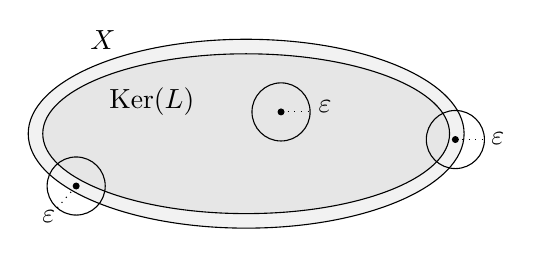
\begin{tikzpicture}[x=0.75pt,y=0.75pt,yscale=-0.7,xscale=0.7]
		%uncomment if require: \path (0,300); %set diagram left start at 0, and has height of 300

		\draw   (374,129) .. controls (374,117.95) and (382.95,109) .. (394,109) .. controls (405.05,109) and (414,117.95) .. (414,129) .. controls (414,140.05) and (405.05,149) .. (394,149) .. controls (382.95,149) and (374,140.05) .. (374,129) -- cycle ;
		\draw  [dotted]  (394,129) -- (414,129) ;
		\draw  [fill={rgb, 255:red, 0; green, 0; blue, 0 }  ,fill opacity=0.05 ] (100,125) .. controls (100,89.1) and (167.16,60) .. (250,60) .. controls (332.84,60) and (400,89.1) .. (400,125) .. controls (400,160.9) and (332.84,190) .. (250,190) .. controls (167.16,190) and (100,160.9) .. (100,125) -- cycle ;
		\draw  [fill={rgb, 255:red, 0; green, 0; blue, 0 }  ,fill opacity=0.05 ] (110,125) .. controls (110,94.62) and (172.68,70) .. (250,70) .. controls (327.32,70) and (390,94.62) .. (390,125) .. controls (390,155.38) and (327.32,180) .. (250,180) .. controls (172.68,180) and (110,155.38) .. (110,125) -- cycle ;
		\draw  [fill={rgb, 255:red, 0; green, 0; blue, 0 }  ,fill opacity=1 ] (392,129) .. controls (392,127.9) and (392.9,127) .. (394,127) .. controls (395.1,127) and (396,127.9) .. (396,129) .. controls (396,130.1) and (395.1,131) .. (394,131) .. controls (392.9,131) and (392,130.1) .. (392,129) -- cycle ;
		\draw   (113,161) .. controls (113,149.95) and (121.95,141) .. (133,141) .. controls (144.05,141) and (153,149.95) .. (153,161) .. controls (153,172.05) and (144.05,181) .. (133,181) .. controls (121.95,181) and (113,172.05) .. (113,161) -- cycle ;
		\draw  [dotted]  (120,176) -- (133,161) ;
		\draw  [fill={rgb, 255:red, 0; green, 0; blue, 0 }  ,fill opacity=1 ] (131,161) .. controls (131,159.9) and (131.9,159) .. (133,159) .. controls (134.1,159) and (135,159.9) .. (135,161) .. controls (135,162.1) and (134.1,163) .. (133,163) .. controls (131.9,163) and (131,162.1) .. (131,161) -- cycle ;
		\draw   (254,110) .. controls (254,98.95) and (262.95,90) .. (274,90) .. controls (285.05,90) and (294,98.95) .. (294,110) .. controls (294,121.05) and (285.05,130) .. (274,130) .. controls (262.95,130) and (254,121.05) .. (254,110) -- cycle ;
		\draw  [dotted]  (274,110) -- (294,110) ;
		\draw  [fill={rgb, 255:red, 0; green, 0; blue, 0 }  ,fill opacity=1 ] (272,110) .. controls (272,108.9) and (272.9,108) .. (274,108) .. controls (275.1,108) and (276,108.9) .. (276,110) .. controls (276,111.1) and (275.1,112) .. (274,112) .. controls (272.9,112) and (272,111.1) .. (272,110) -- cycle ;

		\draw (417,122.4) node [anchor=north west][inner sep=0.75pt]    {$\varepsilon $};
		\draw (141,52.4) node [anchor=north west][inner sep=0.75pt]    {$X$};
		\draw (154,91.4) node [anchor=north west][inner sep=0.75pt]    {$\mathrm{Ker}( L)$};
		\draw (108,176.4) node [anchor=north west][inner sep=0.75pt]    {$\varepsilon $};
		\draw (298,100.4) node [anchor=north west][inner sep=0.75pt]    {$\varepsilon $};
		\end{tikzpicture}
	\end{figure}
	\FloatBarrier
	Then\footnote{Remember that saying that $\forall x\in X,\forall \varepsilon  >0,\exists \, z\in \Ker(L) ,z\in B( x,\varepsilon )$ is a way to say that $\Ker(L)$ is dense in $X$.} $\overline{\Ker(L)}=X$, which is a contradiction.
\end{proof}


\paragraph{Duality in $L^p$ spaces} The following two theorems, the first for the case $p \in (1, \infty)$ and the second for the case $p=1$, discuss duality for functional spaces $L^p$.

Notice that if we are working on $L^p$, with $p \in (1, \infty)$, then we can find $g \in L^q$ for which
$$
	Lg(f)
	= \int_\Omega f g \, \dmu
	\quad \text{where }Lg \in (L^p)^\star
	.
$$

The following theorem goes further providing a complete characterization.

\begin{theo}\label{theo-duality-l-p-1-infinity}
	Let $(\Omega, \mm, \mu)$ a complete measure space.\\
	Consider $L^p(\Omega, \mm,\mu)$ for any fixed $p \in (1, \infty)$.\\
	If $\Lambda \in (L^p(\Omega, \mm, \mu))^\star$ then there exists a unique $g \in L^q(\Omega, \mm, mu)$ where $q$ is the conjugate index of $p$, such that:
	$$\Lambda (f) = \int_\Omega f g \dmu \quad \forall f \in L^p(\Omega, \mm, \mu).$$
	Moreover, we have:
	$$\norm{\Lambda}_{(L^p(\Omega, \mm, \mu))^\star} = \norm{g}_{L^q(\Omega, \mm, \mu)}.$$
	Hence $(L^p(\Omega, \mm, \mu))^\star$ and $L^q(\Omega, \mm, \mu)$ are isometrically isomorphic through $T: \Lambda \mapsto g$.
\end{theo}

This one instead develops the case in which $p = 1$ and $q = \infty$.

\begin{theo}\label{theo-duality-l-p-1}
	Let $\Omega \in \Lc(\RR^N)$ and consider $L^1(\Omega, \Lc(\Omega), \lambda)$.\\
	If $\Lambda \in (L^1(\Omega, \mm, \mu))^\star$ then there exists a unique $g \in L^\infty(\Omega, \mm, \mu)$ such that:
	$$\Lambda (f) = \int_\Omega f g \dmu \quad \forall f \in L^1(\Omega, \Lc(\Omega), \lambda).$$
	Moreover, we have:
	$$\norm{\Lambda}_{(L^1(\Omega, \Lc(\Omega), \lambda))^\star} = \norm{g}_{L^\infty(\Omega, \Lc(\Omega), \lambda)}.$$
	Hence $(L^1(\Omega, \mm, \mu))^\star$ and $L^\infty(\Omega, \mm, \mu)$ are isometrically isomorphic through $T: \Lambda \mapsto g$.
\end{theo}

Pay attention to the main difference: the second result only holds in $\RR^N$ with the Lebesgue measure, while the first one holds in a general metric space.

We need more tools to discuss the case $p=\infty$, we will come back to this at page \pageref{paragraph-duality-p-infinity}.

%!TEX root = ../main.tex
\subsubsection{Hahn--Banach theorem and consequences}
In this section we see the first very relevant theorem for dual spaces: we will see some of its implications, which are many. It was proved by these two mathematician independently in late Twenties. Here is reported the analytic version, but it was also proved a geometric version.\footnote{For further discussion, see: H. Brezis, Functional Analysis, Sobolev Spaces and Partial Differential Equations, 2010, page 4, section 1.2.}
\begin{theo}[Hahn--Banach]
	Let $(X, \norm{\cdot})$ be a real normed vector space and $Y \subset X$ a non-empty subspace. \\
	If $L_0 : Y^\star \to \RR$ then there exists $L \in X^\star$, called the extension of $L_0$ such that:
	$$
		\norm{L}_{X^\star} 
		= \norm{L}_{Y^\star}, 
		\quad L|_Y 
		= L_0
		.
	$$
\end{theo}

\begin{proof}
	
	\textit{First step: construct an extension by adding a dimension to the original subspace.}\\
	Let $x \notin Y$ and set the following:
	$$Z_1 = \{y + \lambda x : \ y \in Y, \ \lambda \in \RR \},$$
	$$L_1 (y + \lambda x) = L_0 y + \lambda \beta,$$
	where $Z$ is a subspace of $X$ and $\beta \in \RR$ is such that we have a control for the norm:
	$$
		|L_1 ( y + \lambda x)|
		=|L_0 y + \lambda \beta|
		\leq \norm{L_0}_{Y^\star} \norm{y + \lambda x}
		,
	$$
	for all $y \in Y$ and all $\lambda \in \RR$. This gives us $\norm{L_1}_{Z^\star_1} \le \norm{L_0}_{Y^\star}$. On the other hand:
	$$Z^\star_1 \supset Y^\star \implies \norm{L_1}_{Z^\star_1} \geq \norm{L_1}_{Y^\star} = \norm{L_0}_{Y^\star}$$
	Hence we have the equality:
	$$\norm{L_1}_{Z^\star_1} = \norm{L_0}_{Y^\star}, \quad L_1|_Y = L_0.$$
	
	\textit{Second step: extension to the complete space.}\\
	Consider now the non-empty family of all possible extensions:
	$$ \Sc = \{ (L,Z): Y \subseteq Z \subseteq X, L \in Z^\star, \norm{L}_{Z^\star} = \norm{L_0}_{Y^\star}, L|_Y = L_0 \}.$$
	Notice that $(L_1, Z_1) \in \Sc$.
	Introduce the partial\footnote{The inclusion induces a partial order: having a set included in the other or viceversa are not the only two possibilities.} order relation:
	$$(L',Z') \leq (L'', Z'') \iff Z' \subset Z'' \text{ with } L''|_{Z'} = L'.$$
	
	Consider a chain (totally ordered subset) $\Cc \neq \varnothing$ of $\Sc$ and set: 
	$$ \tilde Z = \bigcup_{Z: (L,Z) \in \Cc} Z.$$
	
	Observe that $\tilde Z$ is a subspace of $X$, since at every step we're adding to the union another subspace.
	
	If $x \in \tilde Z$ then $x$ belongs to some $Z$ such that $(L,Z) \in \Cc$ and also to all $Z'$ such that $(L', Z') \in \Cc$ and $Z \subset Z'$.\\
	Recalling that $L'|_Z = L$ we can define a linear bounded operator $\tilde L : \tilde Z \to \RR$ by setting:
	$$\tilde Lx = Lx,$$
	where $L$ is associated to the $Z$ where we first encounter $x$.\\
	It's clear that $(\tilde L, \tilde Z)$ is an upper bound for $\Cc$.\\
	Hence $\Sc$ is an inductive set (see definition \vref{chain-defn}) and, by Zorn's Lemma (see proposition \vref{lemma-zorn}), it has a maximal element, namely $(L^\cdot, Z^\cdot)$.\\
	Suppose that $Z^\cdot \subsetneqq X$, then we can construct (see the beginning of this proof) an extension of $(L^\cdot, Z^\cdot)$ but this contradicts its maximality.\\
	Thus $Z^\cdot = X$ and $L^\cdot$ is the required extension.
\end{proof}

Notice that we did not even require completeness for $X$.

% \begin{prop}
% 	If $Y$ is dense in $X$ and $X$ is a Banach space, then $L_0 : Y^\star \to \RR$ has a unique extension $L: X^\star \to \RR$.
% \end{prop}
% 
% In general there is not any necessary and sufficient condition to uniqueness.

% \begin{proof}\todo{check accurately this proof}
% 	Let $x \in X \setminus Y$. Then there exists a sequence $\{y_n\} \subset Y$ such that $y_n \to x$. Thus:
% 	$$|L_0y_n - L_0y_m| \leq M\norm{y_n - y_m}$$
% 	Therefore $\{L_0 y_n\}$ is a Cauchy sequence and there exists $\beta \in \RR$ such that $Ly_n \to \beta$.
% 	
% 	Defining $Lx=\beta$, we have that $|Lx|\leq M \norm{x} \enspace \forall L \in X^\star$, and $L|_y =L_0 \enspace \forall x \in X$
% \end{proof}

%\begin{exam}
%	Consider $X = L^\infty(\RR)$, $Y = C_c(\RR) \subset X$. Let $L_0 f \coloneqq f(0) \quad \forall f \in Y$. \\
%	$L_0$ is linear and $|L f| \leq \norm{f}_\infty \ (M=1) \enspace \forall f \in X$
%	
%	Applying Hahn--Banach theorem, we deduce that:
%	$$\exists \, L \in (L^\infty)^\star : \quad L |_y =L_0 \ \wedge \ |Lf| \leq \norm{f}_\infty \quad \forall f \in X$$
%	
%	However, there does not exist $g \in L^1(\RR)$ such that $L f = \int_{\RR} f g \,\dlam$. \\
%	Indeed, consider $f \in \Cc(\RR)$ such that $f(0) = 0$. If we assume that a suitable $g$ exists, then $\int_{\RR} f g \dlam = 0$. This implies $g=0$ a.e. in $\RR$,\todo{proved at recitation} but then $L \equiv 0$, which is a contradiction.
%	
%	$$(L^\infty(\RR))^\star \supsetneq \todo{???}Y
%	= \left\{ L_g \in (L^\infty)^\star: \enspace L_g f = \int_\RR f g \,\dlam \quad \forall f \in L^\infty (\RR) \right\}$$
%\end{exam}

\paragraph{Relevant consequences} Using the Hahn--Banach theorem we can prove the following three corollaries.

\begin{coro} \label{prop-conseq-HB-1}
	If $x \in X$, with $x\neq 0$, then there exits $L_x \in X^\star$ such that $\norm{L_x}_{X^\star} = 1$ and $L_xx = \norm{x}$.
\end{coro}

\begin{proof}
	Let $Y  \{\lambda x : \lambda \in \RR \}$ and $L_0(\lambda x) = \lambda \norm{x}$. \\
	So $L_0$ is linear and $|L_0(\lambda x)| \leq \norm{\lambda x} \; (M=1)$.\\	
	Notice that $\norm{L_0}_{(Y)^\star}= 1$ so we can simply apply Hahn-Banach theorem.
\end{proof}

\begin{coro} \label{prop-conseq-HB-2}
	Let $x,z \in X$ are such that $Lx=Lz$ for all $L \in X^\star$.\\
	Then $x=z$, that is the elements of $X^\star$ separate the points in $X$.
\end{coro}

\begin{proof}
	By contradiction: let $\tilde x = x-z \neq 0$. Then, using the previous corollary, we find $L\in X^\star$ such that $L\tilde x = \norm{x} \neq 0$, and $Lx \neq Lz$, which is absurd.
\end{proof}

\begin{coro} \label{prop-conseq-HB-3}
	Let $Y \subsetneq X$ be a closed subspace and $x\notin Y$. \\
	Then $L \in X^\star$ such that $Lx \neq 0$ and $L|_Y =0$.
\end{coro}

\begin{proof}
	Let
	$$Z = \{y+\lambda x : y \in Y, \lambda \in \RR\} \subset X \text{ and } L_0(\lambda x  + y) = \lambda.$$
	Then $L_0$ is linear, $L_0 x = 1 \neq 0$, and $\Ker(L_0)= Y$ is closed.\\
	Thus $L_0$ is bounded on $Z$ (due to \vref{theo-charact-bdd-functionals}), and we can apply Hahn--Banach theorem getting the thesis.
\end{proof}

\paragraph{Duality in $L^p$ spaces}\label{paragraph-duality-p-infinity} In the previous chapter we discussed duality when $p\in(1,\infty)$ (\vref{theo-duality-l-p-1-infinity}) and when $p=1$ (\vref{theo-duality-l-p-1}), now with these results we can discuss the remaining case: $p=\infty$.

Consider a function $g\in L^1(\Omega, \Lc(\Omega), \lambda)$, we set:
$$\Lambda_g(f) = \int_\Omega f g \dlam \quad \forall f \in L^\infty(\Omega, \Lc(\Omega), \lambda).$$
We have that $\Lambda_g(f) \in (L^\infty(\Omega, \Lc(\Omega), \lambda))^\star)$ with the norm:
$$\norm{\Lambda_g}_{(L^\infty(\Omega, \Lc(\Omega), \lambda))^\star} = \norm{g}_{L^1(\Omega, \Lc(\Omega), \lambda)}.$$
Observe that the isometry $T: g \mapsto  \Lambda_g$ is not surjective. Indeed, consider $L:(\Cc_C(\RR^N), \norm{\cdot}_\infty) \to \RR$ defined by
$$L(f) = f(0) \quad \forall f \in \Cc_C(\RR^N).$$
Thanks to the Hahn--Banach theorem, $L$ can be extended to an element $\Lambda \in (L^\infty(\RR^N))^\star$.
However, there is no $g \in L^1(\RR^N)$ such that: $$\Lambda(f) = \int_{\RR^N}fg \dlam \quad \forall f \in L^\infty(\RR^N).$$

Suppose that such $g \in L^1(\RR^N)$ exists. Then:
$$\int_{\RR^N} fg \dlam = 0 \quad \forall f \in \Cc_C^\infty(\RR^N) \text{ such that } f(0) = 0.$$

We have the following result which is analogous to the vanishing lemma.
\begin{prop}
	If $\Omega \subseteq \RR^N$ is an open set and $u \in L^1(\Omega)$ is such that: $$\int_\Omega f u \dlam = 0 \quad \forall f \in \Cc_C^\infty (\Omega)$$
	then $u=0$ almost everywhere in $\Omega$.
\end{prop}

Reloading the previous discussion we can take $\Omega = \RR^N \setminus\{0\}$ and conclude $g=0$ almost everywhere in $\RR^N$.\\
Therefore $L(f) = f(0) = 0$ for all $f \in \Cc_C^\infty (\RR^N)$, and we have a contradiction.

%!TEX root = ../main.tex
\subsubsection{Reflexivity}
Since from a space we have constructed its topological dual, we can construct the topological dual of this last one. This is called bidual as we will state soon. But how many times we can redo this process? At a certain point must we stop? Sometimes yes, because the bidual is very similar to the original space, or even it can be the original space itself.

\begin{defn}
	Consider $(X, \norm{\cdot})$ be a real normed vector space.
	The dual of its dual, namely $(X^{\star\star}, \norm{\cdot}_{\star\star})$, is called \emph{bidual}.
\end{defn}

Now we will try to figure out how $X^{\star\star}$ is related to $X$?

Fix $x\in X$ and let
$$\Lambda_x : X^\star \to \RR, \ 
\Lambda_x L\mapsto Lx
\quad \forall L \in X^\star.$$
Observe that $\Lambda_x$ is linear and also bounded: indeed, we have: 
$$|Lx|\leq \norm{L}_\star \norm{x} \quad \forall L \in X^\star.$$
Thus we have $\Lambda_x \in X^{\star\star}$ and $\norm{\Lambda_x}_{\star\star} \leq \norm{x}$.

Moreover, we can find $L\in X^\star$ such that $\norm{L}_\star = 1$ and $Lx=\norm{x}$ (see corollary \vref{prop-conseq-HB-1}), and thus the maximum is achieved:
$$\norm{\Lambda_x}_{\star \star} = \norm{x}.$$

\begin{defn}
	Let  $\tau : X \to X^{\star\star}$ a map defined as $\tau x = \Lambda_x$ where
	$\Lambda_x L\mapsto Lx$ $\forall L \in X^\star$.
	Then $\tau$ is a linear isometry called \emph{canonical map}, and we have:
	$$\norm{\Lambda_x}_{\star\star} = \norm x.$$
\end{defn}

Observe that $\tau(X)$ is a closed subspace of $X^{\star\star}$ but it does no coincide with it in general. 
If they coincide we have:

\begin{defn}
	A normed vector space $X$ linearly isomorphic and isometric to $X^{\star\star}$ is said to be \emph{reflexive}.
In that case we have:$$\tau(X) = X^{\star\star}.$$
\end{defn}

There are some Banach spaces $X$ which are not reflexive, but are linearly isometric and isomorphic to $X^{\star\star}$ through a different isomorphism.\footnote{This was proved by R. C. James in 1951}\\
Moreover observe that any finite dimensional Banach space $(X,\norm{\cdot})$ is reflexive as they are linear isomorphic to $(\RR^N, \norm{\cdot}_2)$.

\begin{prop}
	If a normed vector space $X$ is reflexive, then it is also a Banach space.
\end{prop}

Indeed, $X$ is isomorphic to its bidual, which is always a Banach space.

\begin{theo} \label{theo-lin-iso-reflex}
	Let $(X,\norm{\cdot})$ be reflexive. \\
	If $X$ is linearly isomorphic to $Y$, then $Y$ is reflexive too.
\end{theo}

\begin{proof}
	Let $J:X \to Y$ be a linear isomorphism, and $L \in X^\star$. Then (see \vref{x-y-isomorphic-dual}) we know that there exists $\tilde J:X^\star \to Y^\star$.
	
	Consider $\tilde \Lambda \in Y^{\star\star}$, $\tilde L \in Y^{\star}$. Observe that
	$$
		\tilde \Lambda \tilde L = \tilde \Lambda \tilde J L
	$$
	We define $\Lambda : X^\star \to \RR, \Lambda \in X^{\star\star}, \ L\mapsto \tilde \Lambda \tilde L$.\\
	Since $X$ is reflexive, there exists a unique $x \in X$ such that $\Lambda L = L x$. So we have
	$$
		\tilde \Lambda \tilde L = \Lambda L = L x = L J ^{-1} y = \tilde L y
	$$.
\end{proof}

\begin{theo}\label{theo-x-ref-iff-x-star-ref}
	A space $X$ is reflexive if and only if $X^{\star}$ is reflexive.
\end{theo}

\begin{proof}\textit{Necessary condition} $\implies$:\\
	By contradiction: suppose $\tau(X) \subsetneq X^{\star\star}$, where $\tau$ is the canonical map.
	Since $\tau$ is an isometry and $X^\star$ is a Banach space (see \vref{theo-Bc-banach}) and thus $\tau(X)$ is a closed subspace (see proposition \vref{prop-isometries}).\\
	Therefore, there exists $G : X^{\star\star} \to \RR$, such that $G\not \equiv 0$ and $G|_{\tau(X)}=0$ (see \vref{prop-conseq-HB-3}).\\
	Observe that $G$ belongs to the tridual of $X$, namely:	$G \in (X^{\star\star})^{\star}$.\\
	We have:
	$$G \Lambda_x = 0 \quad \forall x \in X,$$
	where $\Lambda_x = \tau x \in \tau(X) \subsetneq X^{\star\star}$.
		
	But $X^\star$ is reflexive, thus $\tau(X^\star) = X^{\star\star\star}$ and, using the canonical map between $X^\star$ and $X^{\star\star\star}$,
	we have that there exists only one $L\in X^\star$ such that: 
	$$G \Lambda_x =
	\Lambda_x L
	\quad \forall \Lambda \in X^{\star\star}$$
	with $L=\tau^{-1}(G)$. 
	
	Finally, using the canonical map between $X^\star$ and $X^{\star\star}$, one can observe that
	$$G \Lambda_x =
	\Lambda_x L=
	Lx = 0
	\quad \forall x \in X.$$
	Therefore $L \equiv 0$ and $G \equiv 0$ as $\norm{L}_\star = \norm{G}_{\star\star\star}$ which is a contradiction.
	
	\textit{Sufficient condition} $\impliedby$:\\
	If $X$ is reflexive then it is linear isometric and isomorphic to $X^{\star\star}$. Thus we can apply the previous problem: $X^{\star\star}$ is reflexive and then $X^{\star} $ is reflexive.
\end{proof}

\begin{theo}
	If $X$ is reflexive, then any closed subspace of $X$ is reflexive.
\end{theo}

\begin{proof}
	Let $Y \subset X$ be a non-empty closed subspace of $X$. $Y$ is a Banach space.\\
	Let also $\Lambda_0 \in Y ^{\star\star}$, and the mapping $\Lambda_{\sharp} : X^\star \to \RR, \ L \mapsto \Lambda_0 (L|_Y) \in \RR$. $\Lambda_{\sharp} \in X^{\star\star}$.
	$X$ is reflexive, and thus there exists a unique $x_0\in X$ such that $\Lambda_{\sharp} L = L x_0$.
	
	Suppose $x_0 \notin Y$ by contradiction. Then we can find $L_0 \in X^{\star}$ such that $L_0 x_0 \neq 0$, $L_0 |_Y =0$ (see proposition \vref{prop-conseq-HB-3}).
	However
	$$L_0 x_0 = \Lambda_{\sharp} L_0 = \Lambda_0 (L_0 |_Y) =0$$

	Contradiction, therefore $x_0 \in Y$.
	
	Now, for any $\tilde L \in Y^\star$, there exists its Hahn-Banach extension $L \in X^\star$, and we have:
	$$\Lambda_0\tilde L = \Lambda_0(L|_Y) = \Lambda_{\sharp} L = L x_0 = \tilde L x_0.$$
\end{proof}

\paragraph{Relation between dual spaces and separability} Now we have the tools to set up a proper discussion on how separability is kept or inherited by the dual.

\begin{theo}
	If $X^\star$ is separable then $X$ is separable as well.
\end{theo}

\begin{proof}
	Let $\{L_n\}_{n\in\NN}\subset X^\star$ be dense in $X^\star$.\\
	Then for any $n \in \NN$, there exists $x_n \in X$ such that $\norm{x_n}=1$ and
	$$|L_n x_n| \geq \frac 1 2 \norm{L_n}_{\star}
	= \frac 1 2 \sup_{\norm{x} = 1} |L_n x|.$$
	Set now:
	$$E = \left\{ \sum_{j=0}^{N} \alpha_j x_i : N \in \NN, \ \alpha_j \in \QQ \right\}$$
	We have $E$ is countable and $Y=\widebar E\subset X$ is a closed subspace.
	
	By contradiction, suppose $Y \subsetneq X$. We find $L \in X^\star$ such that $L\not\equiv 0$ and $L|_Y =0$ (see corollary \vref{prop-conseq-HB-3}). Since $\{L_n\}_{n\in\NN}$ is dense, we have:
	$$\forall \eps > 0 \quad \exists\, n_0 \in \NN : \enspace \norm{L-L_{n_0}} < \eps.$$
	But the corresponding $x_{n_0}$ belongs to $E \subseteq Y$, and thus $Lx_{n_0} = 0$. Therefore:
	\begin{align*}
		\frac 1 2 \norm{L_{n_0}}_\star &\leq |L_{n_0}x_{n_0}|= |L_{n_0}x_{n_0}-Lx_{n_0}|\\
		&\leq \norm{L_{n_0}-L}_\star\norm{x_{n_0}} < \eps.
	\end{align*}
	Summing up, we have
	$$\norm{L}_{\star} \leq \norm{L-L_{n_0}}_\star + \norm{L_{n_0}}_\star \leq \eps + 2 \eps \quad \forall \eps > 0$$
	and thus $L \equiv 0$, which is a contradiction.
\end{proof}

\begin{theo}\label{x-sep-ref-then-x-star-sep}
	If $X$ is separable and reflexive then $X^\star$ is separable.
\end{theo}

\begin{proof}
	If $X$ is reflexive and separable, then immediately we have that $X^{\star\star}$ is separable, you can check this.\\
	Then, from the previous point, $X^\star$ is separable.
\end{proof}



\paragraph{Reflexivity on $L^p$ spaces} Also for functional spaces we can have reflexivity.\\
Indeed, we can show that $L^p(\Omega, \mm, \mu)$ is reflexive for any $p \in (1,\infty)$.\\
In general $L^1(\Omega, \mm, \mu)$ and $L^\infty(\Omega, \mm, \mu)$ are not reflexive. Consider the case $\Omega=\RR$ with the Lebesgue measure, $L^1$ is separable but $L^\infty$ is not. If $L^1$ were reflexive, it's separable, then (\vref{x-sep-ref-then-x-star-sep}) $(L^1)^\star$ would be separable. This would make $L^\infty \approx (L^1)^\star$ separable, which is false. On the other hand, if $L^\infty$ were reflexive, then $(L^1)^\star$ would be reflexive, then (\vref{theo-x-ref-iff-x-star-ref}) also $L^1$ would be reflexive: this is false as we've just seen.

\paragraph{Sufficient condition for reflexivity} We know that if $X$ is reflexive, then any bounded sequence contains a weakly-converging subsequence.\\
We can apply the first consequence of the Hahn--Banach theorem (see proposition \vref{prop-conseq-HB-1}),
to $X^{\star\star}$, $\forall L \in X^\star \enspace \exists \, \Lambda_L \in X^{\star\star}$
with norm 1 and such that $\Lambda_L L = \norm L_{\star}$.\\
If $X$ is reflexive, then $\forall L \in x^\star \enspace \exists \, x = \tau^{-1} (\Lambda_L)$ with
norm 1 and s.t. $Lx = \Lambda_L L = \norm L_{\star}$, \textit{i.e.} one for which the norm is attained.

\begin{defn}
	Consider a real Banach space $(X, \norm{\cdot})$.\\
	We say that $X$ is \emph{strictly convex}, s.c., if for all distinct $x,y \in X$ such that $\norm{x}\leq 1$ and $\norm{y}$ it follows: 
	$$
		\norm{\frac{x+y}{2}} 
		< 1
		.
	$$
	We say that $X$ is \emph{uniformly convex}, u.c., if for all $\varepsilon > 0$ there exists $\delta > 0$ such that, if $x, y \in X$ are such that $\norm{x} \leq 1$, $\norm{y} \leq 1$, $\norm{x-y} > \varepsilon$ then 
	$$
		\norm{\frac{x+y}{2}}
		< 1 - \delta
		.
	$$
\end{defn}
This last property entails that if two points $x$ and $y$ are in the closed unit ball, even on the boundary, then their mean point must lie deep inside that same unit ball.

Observe that a uniform convex space is also strictly convex.

The space $(\RR^N, \norm{\cdot}_p)$ with $N \geq 2$ is uniformly convex if and only if $p \in (1,\infty)$, but for $p=1$ and $p=\infty$ is not even strictly convex.

It can be shown that, given a real normed vector space $X$, the Hahn--Banach extension is unique if $X^\star$ is strictly convex.\footnote{A.E. Taylor proved in 1939 that the condition is sufficient while S. Foguel in 1958 proved that is also necessary.}

\begin{theo}[Milman--Pettis]\label{theo-milman-pettis}
	Any real uniform convex Banach space is reflexive.
\end{theo}

The converse is not true. More precisely, there are some infinite-dimensional reflexive Banach spaces which are not linearly isomorphic to a uniformly convex space.\footnote{Proven by M.M. Day in 1941.}

Remember that any finite-dimensional Banach space is reflexive: uniform continuity isn't, indeed, a necessary condition.

Now consider the $\RR^N$ cases; the spaces $(\RR^2, \norm{\cdot}_\infty)$ and $(\RR^2, \norm{\cdot}_1)$ both have ``square'' unit balls: we can check that they are not uniformly convex spaces.\\
However, we know that both of them are reflexive and linearly isomorphic to $(\RR^2, \norm{\cdot}_2)$ which is uniformly convex.
Indeed,	we can prove that $(\RR^N, \norm{\cdot}_2)$ is reflexive for any $n$.\footnote{This via uniform convexity, via equivalence of weak and strong convergence and Bolzano-Weierstrass' theorem or via James' theorem.}\\
Spaces $L^p(\Omega,\mm,\mu)$ with $p \in (1,+\infty)$ are reflexive.

\paragraph{Clarkson's inequalities}We could also prove it via Milman--Pettis and the following inequalities.

\begin{prop}
	Let $f,g \in L^p(\Omega, \mm, \mu)$ with $p \in (1, \infty)$.\\
	The \emph{Clarkson's inequalities} holds:
	\begin{align*}
		\norm{\frac{f+g}{2}}_p^p +
		\norm{\frac{f-g}{2}}_p^p
		&\le \frac 1 2
		\left( \norm f_p^p + \norm g_p^p \right) \quad
		&p \in [2,\infty)
		\\
		\norm{\frac{f+g}{2}}_p^q + 
		\norm{\frac{f-g}{2}}_p^q
		&\le \left( \frac 1 2 \norm f_p^p + 
		\frac 1 2 \norm g_p^p \right)^{\nicefrac q p} \quad
		& p \in (1,2)		
	\end{align*}
	Where $q$ is $p$'s conjugate.
\end{prop}

\paragraph{Characterization of reflexivity} As we have seen uniform convexity is only a sufficient conditions but there exist some necessary and sufficient conditions for reflexivity.

\begin{theo}[James]
	Let $X$ be a Banach space.
	Then $X$ reflexive if and only if any $L \in X^\star$ has a maximum on the unit ball.
\end{theo}

The implication is trivial: if $L\in X^\star$ then by applying HB first corollary (\vref{prop-conseq-HB-1}) on $X^{\star}$ there exists $\Lambda \in X^{\star\star}$ such that $\norm{\Lambda}_{\star\star} =1$ and $\Lambda L=\norm{L}_\star$; therefore, for $x = \tau^{-1}(\Lambda)$ we have $Lx=\norm{L}_\star$ with $\norm{x} = 1$.


%$X$ is reflexive if and only if $\forall L \in X^\star \exists \, x \in X$ with norm 1 such that:
%$$Lx = \norm L_\star = \max_{\norm{\widetilde x} = 1} L \widetilde x$$
%For $(\RR^N, \norm{\cdot}_2)$ we know that any $L \in (\RR^N)^\star$ has a unique representation vector $\vec a \in \RR^N$ such that $L \vec x = \sca{\vec a, \vec x}$.
%Choosing $\vec x = \frac{\vec a}{\norm{\vec a}}$, we get:
%$$L \vec x = \frac{\norm{\vec a}^2}{\norm{\vec a}} = \norm{\vec a} = \norm L_\star$$
%The norm is attained and thus $(\RR^N, \norm{\cdot}_2)$ is reflexive.



%%%%%%%%%%%%%%%%%%


















%!TEX root = ../main.tex
\subsubsection{Weak convergence}
From now on, let $(X, \norm{\cdot})$ be a Banach space.
\begin{defn}
	We say that he sequence $\{x_n\} \subset X$ \emph{weakly converges} to $x \in X$ if, for all $ L \in X^\star$ we have:
	$$L x_n \to L x \text{ as }  n \to \infty;$$
	in such case we will write:
	$$x_n \wto X.$$
\end{defn}

From now on, we will refer to $x_n \to x$ as \emph{strong convergence}.\\
Observe that the strong convergence implies the weak one. Indeed, if $x_n \to x$ in $X$, then $|Lx_n-Lx| \leq \norm{L}_\star \norm{x_n-x} \to 0$ for any $L \in X^\star$, and thus $x_n \wto x$.\\
In general, the converse is not true; consider the following example:
\begin{exam}
	Take $X=L^2([-1,1])$ and let $f_n(t) = \sin(nt)$, with $n \in \NN$.\\
	Clearly $f_n \not \to 0$, but it is easy to prove that $f_n \wto 0$: since $(L^1)^\star \approx L^\infty$, 
	we have:
	$$\int_{-1}^1 f_n(t) g(t) \, \dt \to 0 \quad \forall g \in L^\infty ([-1,1]).$$
	Check this as an exercise.
\end{exam}

You can show also that if $X$ is finite dimensional then the converse holds.\\
Indeed: consider $(\RR^N, \norm{\cdot}_2)$. If $x_n \wto x$, then $L x_n \to L x \enspace \forall L \in (\RR^N)^\star$. \\
But, $\forall L \in (\RR^N)^\star$, $\exists! \ a \in \RR^N: L y=\sca{a, y}$, thus:
$$\sca{a, x_n} \to \sca{a, x} \quad \forall a \in \RR^N$$
Taking $ a = e_j$, we have $x_n^j \to x^j$, i.e. strong convergence in each coordinate.

This implies that $x_n \to x$ in $\norm{\cdot}_\infty$ so, by equivalence: $ x_n \to x$ in $\norm{\cdot}_2$ and in every norm which makes $\RR^N$ a Banach space.

By isometry, we deduce that in any finite dimensional Banach space the weak convergence implies the strong one.

Finally notice that weak and strong convergence are equivalent in $l^1$.%\footnote{Proven by Schur.}

\paragraph{Basic properties} We can easily deduce some properties of this new kind of convergence.

\begin{prop}
	The weak limit is unique.
\end{prop}
\begin{proof}
	Suppose $(x_n \wto x) \wedge (x_n \wto \tilde x)$ with $x \neq \tilde x$.\\
	Then for any $L \in X^\star$, $(Lx_n \to L x )$ and $(Lx_n \to L\tilde x)$.\\
	The strong limit is unique, so $Lx = L\tilde x$ for any $L \in X^\star$, and finally using HB second corollary \vref{prop-conseq-HB-2} we get $x = \tilde x$.
\end{proof}

\begin{prop}
	If $x_n \wto x$, then $\{x_n\}$ is bounded in $X$.
\end{prop}
\begin{proof}
	A sequence $\{Lx_n\}$ is bounded for each $L \in X^\star$ since it's a convergent sequence in $\RR$.\\
	Set $T_n L = L x_n$ for any $L \in X^\star$.
	Applying the uniform boundedness principle (see theorem \vref{theo-banach-steinhaus}) to $\{T_n\} \subset X^\star$ we have that there exists $M>0$ such that: $$\norm{T_n}_{\star\star} \leq M.$$
	Moreover, for each $n \in \NN$, we can find (\vref{prop-conseq-HB-1}) $L_n \in X^\star$ such that $\norm{L_n}_\star = 1$ and $L_nx_n = \norm{x_n}$.
	So we have: $$\norm{x_n}= |L_nx_n| = |T_nL_n| \leq \norm{T_n}_{\star\star} \underbrace{\norm{L_n}_\star}_{=1} \leq M.$$
\end{proof}

\begin{prop}
	The norm function is lower semi-continuous with respect to the weak convergence, namely if $x_n \wto x$ then: $$\norm{x} \leq \liminf\limits_{n\to\infty} \norm{x_n}.$$
\end{prop}
\begin{proof}
	Using HB first corollary (\vref{prop-conseq-HB-1}), let $L \in X^\star$ such that norm $\norm{L} = 1$ and $Lx = \norm{x}$. We have that:
	$$0 < \norm{x} = L x
	= \lim_{n\to +\infty}L x_n
	= \lim_{n\to +\infty}|L x_n|
	= \liminf_{n\to +\infty}|L x_n|\leq \liminf_{n\to\infty}\norm{x_n}.$$
	We can put the absolute value in $|Lx_n|$ because the limit is the norm of $x$, which is non negative.
\end{proof}

\begin{prop}
	If $x_n \wto x$ and $L_n \xrightarrow{X^\star} L$, then $L_n x_n \to L x$.
\end{prop}
\begin{proof} As $n \to +\infty$ we have:
	\begin{align*}
		L_n x_n - L x_n &= |(L_n-L)|x_n \leq \norm{L_x -L}_\star M \to 0 \\
		&\\
		L_n x_n - Lx &= L_n x_n - L x_n + Lx_n - Lx \\
		&= (L_n x_n - L x_n) + L(x_n - x) \to 0.
	\end{align*}
\end{proof}

What happens to the weak convergence when $Y\neq \RR$? We have the following result.

\begin{prop}
	Let $X$, $Y$ be Banach spaces and $T \in \Bc(X,Y)$.
	Then $ x_n \wto x$ implies $T x_n \wto Tx$.
	In this case we say that $T$ is \emph{weak-weak continuous}. 
	\label{prop-bdd-weak-weak}
\end{prop}
\begin{proof}
	Let $L \in Y^\star$.\\
	The mapping $x \mapsto LTx$ is an element of $X^\star$.\\
	Now set $\Lambda x = L T x$ with $\Lambda \in X^\star$.\\
	We have $\Lambda x_n \to \Lambda x$ as $x_n \wto x$; so we have:
	$$LTx_n \to LTx \quad \forall L \in Y^\star$$
	that is the definition of $Tx_n \wto Tx$.
\end{proof}

\begin{prop}
	Let $X$ be reflexive.
	If $\{Lx_n\}$ converges for any $L \in X^\star$, then there exists a unique $x \in X$ such that $x_n \wto x$.
\end{prop}
\begin{proof}
	Fix $n\in \NN$, then let $\{T_n\}_{n\in \NN}\subset X^{\star\star}$ such that $T_nL = L x_n$ for each $L \in X^\star$.\\
	We have (see corollary \vref{coro-UBP-conv}) that $\{T_n\}$ converges point-wise to some $T \in X^{\star\star}$.\\
	Setting $x = \tau^{-1}(T)$ we have $Lx_n = T_n L \to TL = Lx$ for any $L \in X^\star$.
	The thesis is proven.	
\end{proof}

\paragraph{Weak$^{\star}$ convergence} Analogously, we can define a weak convergence notion also for functionals.
\begin{defn}
	We say that $\{L_n\}\subset X^\star$ \emph{weakly$^\star$ converges} to $L \in X^\star$ if, for all $x \in X$ we have:
	$$L_n x \to Lx\text{ as }n \to \infty;$$
	in such case we will write:
	$$L_n \wsto L.$$
\end{defn}

In $X^\star$, both weak convergence and weak$^\star$ convergence are defined, but the latter is weaker. Indeed:
\begin{alignat*}{4}
	L_n \wsto L && \iff & \; L_n x \to L x \quad &&\forall L\in X \\
	L_n \wto L && \iff & \; \Lambda L_n \to \Lambda L \quad &&\forall \Lambda\in X^{\star\star} \vphantom{\wsto} \\
	L_n \wsto L && \implies & \; \Lambda L_n \to \Lambda L \quad &&\forall \Lambda \in \tau(X)
\end{alignat*}
where $ \Lambda L_n = L_n x$, $ \Lambda L = L x$. Therefore, such convergences are equivalent if and only if $\tau(X)=X^{\star\star}$, that is if and only if $X$ is reflexive.
 
If $X$ is not reflexive we still have $L_n \wto L \implies L_n \wsto L$.


Arguing as before we have the following properties
\begin{prop}
	\Fixvmode
	\begin{itemize}
		\item The weak$^\star$ limit is unique;
		\item If $L_n \wsto L$ then $\{L_n\}$ is bounded in $X^\star$;
		\item The norm is lower semi-continuous with respect to the weak$^\star$ convergence, that is, if $L_n \wsto L$ then $\norm{L}\leq \liminf\limits_{n \to \infty}\norm{L_n}_\star$;
		\item If $(x_n \to x)$ and $(L_n \wsto L)$ then $L_x x_n \to L X$.
	\end{itemize}
\end{prop}

\paragraph{A weak$^\star$ compactness criterion}

\begin{theo}[Banach--Alaoglu] \label{theo-banach-alaoglu}
	Let $X$ be a separable Banach space. \\
	Then any bounded sequence $\{L_n\}_{n \in \NN} \subset X^\star$ contains a subsequence which weakly$^\star$ converges to some $L\in X^\star$.
\end{theo}

Separability is necessary, consider the following example.
\begin{exam}
	Take $X = l^\infty$ and $\{L_n\}_{n\in\NN} \subset X^\star$ such that:
	$$L_n x = x_n \quad \forall x = \{x_n\}_n \in l^\infty.$$
	Notice that $L_n$ is obviously bounded, namely $\norm{L_n}_\star \le 1$, because $\abs{L_n x} \le \norm{x}_\infty$. \\
	Anyway $L_n$ does not contain any weakly$^\star$ convergent sub-sequence: if there exists any $\{L_{n_k}\}_k$, taking $x = \{(-1)^{n_k}\}_{n_k \in \NN}$ we reach a contradiction $L_{n_k} x = (-1)^{n_k}$ does not converge as $n \to +\infty$.
\end{exam}

\begin{proof}
	First, let $M = \sup_{n\in\NN}\norm{L_n}_\star \in [0, +\infty)$.\\
	Consider a sequence $\{x_k\}_{k\in \NN} \subset X$ dense in $X$.\\
	Take the sequence $\{L_n x_0\}_{n \in \NN} \subset \RR$ which is bounded. By Bolzano--Weierstrass theorem (\vref{bolzano-weierstrass-theo})  there exists a converging subsequence $\{L_{n_{j_0}}x_0\}_{j_0 \in \NN}$.\\
	Take also the bounded sequence $\{L_{n_{j_0}} x_1\}$: there exists a converging subsequence $\{L_{n_{j_1}} x_1\}_{j_1 \in \NN}$.\\
	
	By diagonalization (see for analogy the proof of Ascoli--Arzelà theorem  \vref{theo-ascoli-arzela}) we can extract $\{L_{n_h}\}_{h \in \NN}$ such that $\{L_{n_j} x_k\}_{j\in \NN}$ converges for any $k \in \NN$ with respect to $j$.
	
	Consider $x \in X$ and fix $\eps >0$. Via separability, we can find $x_k$ such that $\norm{x-x_k}\leq \frac{\eps}{2M}$.

	Observe now that:
	$$ |L_{n_i}x-L_{n_j}x| \leq |L_{n_i} x - L_{n_i}x_k|+|L_{n_i}x_k-L_{n_j}x_k|+|L_{n_j}x_k-L_{n_j}x|. $$
	We have:
	\begin{align*}
		|L_{n_i} x - L_{n_i}x_k| &\leq M \norm{x-x_k}\leq \tfrac \eps 2, \\
		|L_{n_j}x_k-L_{n_j}x| &\leq M \norm{x-x_k}\leq \tfrac \eps 2.
	\end{align*}
	Moreover, $\{L_{n_j} x_k\}_{j\in\NN}$ converges as it is a fundamental sequence, and we can find $j' \in \NN$ such that:
	$$|L_{n_i} x_k - L_{n_j}x_k | \leq \eps \quad \forall i,j \geq j'.$$
	Summing up:
	$$|L_{n_i}x-L_{n_j}x| \leq 2 \eps \quad \forall i, j \ge j'.$$

	Therefore $\{L_{n_j} x\}$ is a Cauchy sequence and converges. Via an implication of the uniform boundedness principle (see corollary \vref{coro-UBP-conv}), there exists $L \in X^\star$ such that $L_{n_j}x \to L x \enspace \forall x \in X$. An this concludes the proof.
\end{proof}

\begin{exam}
	Consider the space $(\Omega, \Lc(\Omega), \lambda)$ with $\Omega \subseteq \RR^N$ and $\lambda(\Omega) >0$, and a sequence $\{f_n\}_{n\in\NN}\subset L^\infty (\Omega)$. \\
	Set: $$L_n(g) = \int_\Omega f_n g \, \dlam \quad \forall g \in L^1(\Omega).$$
	If $\{f_n\}_{n\in\NN}$ is bounded, then $\{L_n\}_{n \in \NN}$ is bounded in $(L^1(\Omega))^\star$.\\
	By Banach--Alaoglu theorem, as $L^1(\Omega)$ is separable, we can extract a subsequence $\{L_{n_h}\}_{h \in \NN}$ which weakly$^\star$ converges to an $L \in (L^1(\Omega))^\star$, namely: $$L_{n_h} (g) \to L(g) \quad \forall g \in L^1(\Omega) \quad \text{as }h \to \infty.$$
	Moreover, we know that exists a unique $f \in L^\infty (\Omega)$ such that:
	$$L(g) = \int_\Omega f g \, \dlam \quad \forall g \in L^1(\Omega).$$
	Therefore the weak$^\star$ convergence can be written in terms of integrals as follows:
	$$\int_\Omega f_{n_h} g \,\dlam \to \int_\Omega f g \,\dlam \quad \forall g \in L^1(\Omega, \mm, \mu) \quad \text{as }h \to \infty.$$
\end{exam}

This is an example of the statement ``for any bounded sequence in $L^\infty(\Omega)$ we can extract a weakly$^\star$ convergent subsequence''.

Remember also that $L^1(\Omega,\mm,\mu)$ is separable if, for instance, $\Omega \in \Lc(\RR^N) = \mm$.
It may not be separable in some extremely pathological cases.



\paragraph{Considering also the reflexivity} Reflexivity is a strong assumption. Can we say more if $X$ is also reflexive?
\begin{prop}
	If $X$ is separable and reflexive, then any of its bounded sequences contains a weakly-converging sub-sequence.
	\label{prop-coro-BA}
\end{prop}
\begin{proof}
	Let $\{x_n\}_{n\in\NN}\subset X$ a bounded sequence.\\
	As $X^\star$ is separable we can apply the Banach--Alaoglu theorem to $\{\tau(x_n)\}_{n \in \NN}\subset X^{\star\star}$, which is bounded since $x_n$ is a bounded sequence and the canonical map is isometric, and find $\{\tau(x_{n_h})\}_{h \in \NN}$ such that $$\tau(x_{n_h}) \wsto \Lambda$$ as $h \to \infty$ for some $\Lambda \in X^{\star\star}$.\\
	Thanks to the reflexivity of $X$ we have that $x = \tau^{-1}(\Lambda)$ and $$x_{n_h} \wto x$$ as $h\to\infty$.
\end{proof}

\paragraph{Another characterization for reflexivity} Actually we can say much more: separability is not necessary in statement \vref{prop-coro-BA}. Moreover the converse holds:
\begin{theo}[Eberlin--Šmulian] \label{theo-eberlin-smulian}
	If $X$ is a Banach space in which any bounded sequence contains a weakly-converging subsequence, then $X$ is reflexive.
\end{theo}

	Let $\{f_n\}_n \subseteq L^p(\Omega, \Lc(\Omega), \lambda)$ with $p \in (1,+\infty)$ and $\lambda(\Omega) > 0$.\\
	We know that $L^p$ is separable, and hence $(L^p)^\star \approx L^q$, with $p,q$ conjugates: operators on $L^p$ can be represented as integrals with an appropriate $L^q$ function.\\
	If $\{f_n\}$ is bounded, then there exists a subsequence $\{f_{n_k}\}$ and a function $f \in L^p$ such that $\int_\Omega f_{n_k} g \,\dlam \to \int_\Omega fg \,\dlam \enspace \forall g \in L^q$, and, in particular, $L_g f = \int_\Omega fg \,\dlam$ and $L_g \in (L^p)^\star \approx L^q$.\\
	Summing up, if $p\in(1,\infty)$, from any bounded sequence in $L^p(\Omega)$ we can extract a weakly convergent subsequence.
%
%\paragraph{A sufficient condition for strong convergence}
%\begin{prop}
%	Let $(X, \norm \cdot)$ be an uniformly convex Banach space. \\
%	If a sequence $\{x_n\}_n \subseteq X$ is such that $x_n \wto x$ and $\limsup_{n} \norm{x_n} \le \norm x$, then $x_n \to x$.
%\end{prop}
%The assumptions of the theorem imply the lower semi-continuity of the norm, namely $\norm x \le \liminf \norm{x_n}$, and thus the convergence of the norm: $\norm{x_n} \to \norm x$.\todo{Ref?}
%
%\begin{proof}
%	The case $x=0$ is trivial. If $x \neq 0$, set $\lambda_n \coloneqq \max\{\norm{x_n}, \norm x\} \enspace \forall n \in \NN$.
%	The convergence of the norm entails that $\lambda_n \to \norm x$.
%	
%	Now set $y_n \coloneqq \frac{x_n}{\lambda_n}$ and $y \coloneqq \frac{x}{\norm x}$.
%	The reader should check that, as $n = +\infty$, $y_n \wto y$.
%	
%	Via the semi-continuity of the norm, since $\frac{y_n + y}{2} \wto \frac{2y}{2} = y$, we have:
%	\begin{align*}
%	\norm y &\le \liminf \norm{\frac{y_n+y}{2}}
%	\intertext{But $\norm y = 1$ and $\norm{y_n} \le 1$, hence:}
%	1 = \norm y &\le \liminf \norm{\frac{y_n+y}{2}} \le \limsup \norm{\frac{y_n+y}{2}} \\
%	&\le \limsup \tfrac 1 2 \norm{y_n} + \tfrac 1 2 \norm{y} \le \tfrac 1 2 + \tfrac 1 2 = 1
%	\end{align*}
%	That is, $\lim_{n} \norm{\frac{y_n+y}{2}} = 1$.
%	
%	Suppose now, by contradiction, that $y_n \not\to y$. Then we can find a non-Cauchy subsequence, namely there exist $\eps_0 > 0$ and $\{y_{n_k}\}$ such that:
%	$$\norm{y_{n_k}-y_{n_k'}} > \eps_0 \quad \forall k,k' \in \NN$$
%	Since $X$ is uniformly convex:
%	$$\exists \, \delta_0 > 0 : \enspace 1-\delta > \norm{\frac{y_{n_k}+y_{n'_k}}{2}} \not\to 1$$ which is a contradiction, and thus $y_n \to y$. Since $\lambda_n \to \norm x$ as well, one has $x_n \to x$.
%\end{proof}
%

%!TEX root = ../main.tex
\subsubsection{Linear compact operators}
Now we see a further property for linear operator. Here we require an improvement of the image of the operator that paves the way to new results.

Throughout this section, let $(X, \norm{\cdot}_X)$, $(Y, \norm{\cdot}_Y)$ be Banach spaces.
\begin{defn}
	A linear operator $K \in \Lc(X,Y)$, $K:X \to Y$ is \emph{compact} if for any bounded set $B \subseteq X$ the image $KB$ is precompact in $Y$, i.e. $\overline{KB}$ is compact.
	Their space is defined as $$\Kc(X,Y) \coloneqq \{ K \in \Lc(X,Y) \text{ compact} \}.$$
\end{defn}

The term precompact means that its closure is compact.

In other words, any bounded sequence $\{y_n\}_n \subseteq KB$ contains a converging subsequence which limit needs not to be in $KB$.

If $X=Y$, then often it is written as $\Kc(X)$.

\begin{prop}
	Any compact operator is bounded.
	\label{prop-compact-bdd}
\end{prop}
\begin{proof}
	Take the unit ball $B = B_1(0) \subseteq X$.\\
	As $KB$ is precompact, $\overline{KB}$ is compact, so it is is also bounded.\\
	Therefore there exists $M > 0$ such that:
	$$
		\norm K_\star 
		= \sup\limits_{x \in \widebar B} \norm{Kx} 
		\le M
	$$ 
	that is, $K \in \Bc(X,Y)$.
\end{proof}

\begin{defn}
	A linear operator is \emph{finite-rank} if its image is finite dimensional. 
\end{defn}

\begin{prop}
	A finite-rank bounded operator is also compact. 	
\end{prop}
Indeed, notice that if $T \in \Bc(X,Y)$ and $Y$ is finite-dimensional then $T$ is compact.\\
However, there are compact operators which are not finite-rank: consider $(C([a,b]), \norm{\cdot}_\infty)$ and, for each $u \in C([a,b])$, set:
$$Ku(t) = \int_a^t u(s) \ds \quad \forall t \in [a,b].$$
The linear operator $K: C([a,b]) \to C([a,b])$ is compact (see Ascoli--Arzelà theorem \vref{theo-ascoli-arzela}), indeed we have $\Im(K)=\{f \in \Cc^1([a,b]): f(a) = 0\}$.

Note also that if $X$ and $Y$ are infinite-dimensional, then $\Kc(X,Y) \subsetneq \Bc(X,Y)$. \\ 
An example of bounded, non-compact operator is the identity map, if $X=Y$ infinite-dimensional.

%\begin{rema}
%	In terms of sequences: $\forall \{ x_n \} \subset X$ bounded $\exists \, \{x_{n_h}\}$ such that $\{ K x_{n_h}\}$ converges to some $y \in Y$
%\end{rema}

\begin{defn}
	If $Y$ is a subspace of $X$ and the identity $I : Y \to X$ is compact we say that $Y$ is \emph{compactly embedded} in $X$ and we write: $$Y \hookrightarrow\hookrightarrow X.$$
\end{defn}

\begin{prop}
	Let $X$ be an infinite dimensional Banach space.\\
	Then a compact operator $K:X \to X$ cannot be bijective.
\end{prop}

\begin{proof}
	By contradiction, take $\{y_n\}_{n \in \NN} \subset B$, where $B$ is the unit ball of $X$.\\
	Consider now $x_n = K^{-1} y_n$: the sequence $\{x_n\}_{n \in \NN}$ is bounded, as $K^{-1}$ is bounded.\\
	Since $\{y_n\}_{n \in \NN}$ contains a convergent sub-sequence, $B$ is compact, which is a contradiction to \vref{theorem-riesz}.
\end{proof}


\paragraph{Characterization for compact operators} To prove directly the compactness is not an easy task, anyway we can find a criterion to do the job.

\begin{theo}[Compactness characterization] \label{theo-compact-charact}
	If $K \in \Kc(X,Y)$ and $x_n \wto  x$, then: $$ K x_n \to Kx.$$
	This means that $K$ is \emph{weak-strong continuous}.
	
	Moreover, if $X$ is reflexive and $K \in \Bc(X,Y)$ is weak-strong continuous, then $K$ is also compact.
\end{theo}


\begin{proof} The two parts will be proved separately.\\
	\textit{Proof of the first part:}\\ 
	Suppose $K \in \Kc(X,Y)$ and $x_n \wto x$. Being also bounded (see \vref{prop-compact-bdd}), $K$ is weak-weak continuous (see \vref{prop-bdd-weak-weak}), namely $Kx_n \wto Kx$.\\
	If $\{x_n\}$ is bounded, we have that $\{Kx_n\}$ is also bounded and contains a strongly convergent subsequence, and $\{Kx_n\}$ has a non-empty and bounded class limit.
	
	Let $y$ be a limit point: there exists $\{K x_{n_h}\}_{h \in \NN}$ such that $Kx_{n_h} \to y$ and in particular $Kx_{n_h} \wto y$.\\
	Therefore $y = Kx$ is the only limit point: we have that $K$ is weak-strong continuous, namely $Kx_n \to Kx$.
	
	\textit{Proof of the second part:}\\ 
	Suppose now that $K \in \Bc(X,Y)$ is weak-strong continuous, consider a bounded set $E \subset X$  and the sequence $\{y_n\}_{n\in\NN} \subset KE$.\\
	Then there exists $x_n \in E$ such that $Kx_n = y_n$ for every $n \in \NN$.\\
	
	Using the reflexivity of $X$ we can apply the corollary \vref{prop-coro-BA} to the BA theorem\footnote{Remember that separability was not necessary, even though to prove it without this assumption, we can't take advantage of the Banach-Alaoglu theorem.} and find $\{x_{n_h}\}_{h \in \NN}$ such that $x_{n_h}\wto x$. Hence $Kx_{n_h} \to Kx$ and $KE$ is precompact. This entails $K \in \Kc(X,Y)$.
\end{proof}

We have seen that $\Kc(X,Y)$ is a subspace of $\Bc(X,Y)$. We are now going to prove that $\Kc(X,Y)$ is closed.

\begin{theo}
	The space of compact operators $\Kc(X,Y)$ is a closed subspace of $\Bc(X,Y)$.\\
	This means that $\Kc(X,Y)$ is a Banach space with respect to the induced norm.
\end{theo}
\begin{proof} \textit{For simplicity, we will prove the theorem when $X$ is also reflexive.}\\
	Consider a converging sequence $\{K_n\}_{n\in\NN} \subset \Kc(X,Y)$, such that there exists: $$K \in \Bc(X,Y) : \enspace \norm{K_n-K}_{\Bc(X,Y)}\to 0 \quad \text{as } n \to +\infty.$$
	We are left to prove that $K$ is compact, namely $K \in \Kc(X,Y)$, by showing that it is weak-strong continuous (see the theorem stating the characterization of the compactness \vref{theo-compact-charact}).
	
	Let $\{x_n\}$ such that $x_n \wto x$; as $\{x_n\}_{n\in\NN}$ is bounded there exists $M > 0$ such that $\norm{x_n}_X \leq M$, and we have:
	\begin{align*}
		\norm{Kx_n - Kx}_Y 
		& \leq \norm{Kx_n-K_j x_n}_Y + \norm{K_jx_n- K_j x}_Y + \norm{K_j x- K x}_Y\\
		& \leq 2M \norm{K-K_j}_{\Bc(X,Y)} + \norm{K_jx_n- K_j x}_Y
	\end{align*}
	Let $\eps > 0$ be fixed. Then exists $j_0 \in \NN$ such that $$\norm{K_j -K}_{\Bc(X,Y)} < \frac{\eps}{3M} \quad \forall j \geq j_0.$$
	Therefore:
	$$\norm{Kx_n - K_j x_n}_Y 
	\leq M \cdot \norm{K-K_j}_{\Bc(X,Y)} < \tfrac \eps 3
	\quad
	\forall j \geq j_0
	.$$
	Moreover, since $x_n \wto x$, via lower semi-continuity we have:
	$$
	\norm{K_jx-Kx}_Y 
	\leq \liminf_n \norm{K_j x_n-Kx_n}_Y \le \tfrac \eps 3
	\quad
	\forall j \geq j_0
	.$$
	Fix $j=j_0$. Since $K_{j_0} \in \Kc(X,Y)$, there exists $n_0 \in \NN$ such that:
	$$
	\norm{K_{j_0}x_n - K_{j_0}x}_Y 
	< \tfrac \eps 3
	\quad
	\forall n \geq  n_0
	.$$
	
	Summing up:
	$$\forall \eps > 0 \quad \exists \, n_0=n_0(\eps) \in \NN : \enspace \norm{Kx_n -Kx}_y < \eps \quad \forall n \geq n_0$$
	Thus $Kx_n \spaceto{Y} Kx$, and $K$ is compact.
\end{proof}

\paragraph{The approximation problem} The previous theorem has an immediate consequence:
\begin{prop}
	If we have a converging sequence of finite-rank linear  operators, then its limit is a compact operator.
\end{prop}
The converse of this proposition is known as \emph{approximation property}: is any $K \in \Kc(X,Y)$ the limit of a sequence of finite rank operators, with respect to the operator norm? 

In general it is not: Per Enflo proved in 1973 that there exists a Banach space which is separable but it does not have any Schauder basis and so the approximation property does not hold.

We know that the approximation property holds if $Y$ has a Schauder basis or if $Y$ is a Hilbert spaces (see definition \vref{defn-hilbert-spaces}).

%neumann series, min 8 of lesson 30/11/2020

\paragraph{First example of compact operator} We are now going to introduce a class of linear compact operators, from $L^p$ to $L^q$.\\
Consider $(\Omega, \Lc(\Omega), \lambda)$ with $\Omega \in \Lc(\RR^N)$
and $G \in L^q(\Omega \times \Omega)$ with respect to the Lebesgue measure in $\RR^{2N}$
for some $q \in (1, \infty)$.

For any $u \in L^p(\Omega)$, where $p$ is the conjugate of $q$, set
$$K_G u(x) = \int_\Omega G(x,y) u(y) \,\dy$$
for all $u \in L^p(\Omega)$ and for almost any $x \in \Omega$.
The function $G$ is called \emph{kernel} of the operator $K_G$.

Using Hölder's inequality we have:
$$
	|K_G u(x)|^q
	\leq \left( \int_\Omega |G(x,y)| \ |u(y)| \,\dy \right)^q
	\leq \norm{G(x, \cdot)}_q^q\norm{u}_p^q
$$
for almost any $x \in \Omega$. This implies that:
$$
	\norm{K_G}_{q}
	\leq \norm{G}_{q} \norm{u}_{p}
	\quad \forall u \in L^p(\Omega)
	.
$$
Then we deduce that $K_G$ is linear and bounded from $X=L^p(\Omega)$ and $Y=L^q(\Omega)$.

%Let us prove that $K_G \in \Kc(X)$; we can use the characterization given by \vref{theo-compact-charact}. %è certamente cannata ma può avere un suo perché
Let $\{u_n\}_{n\in \NN} \subset L^p(\Omega)$ be such that $u_n \wto u$.\\
Define the converging sequence:
$$\Phi_n(x) = K_G(u_n - u)(x) = \int_\Omega G(x,y)(u_n - u)(y) \, \dy \to 0$$
for almost any $x \in \Omega$. Notice that we have:
$$|\Phi_n(x)|^q \leq \norm{G(x, \cdot)}^q_q \norm{u_n - u}_q^q \leq M \norm{G(x, \cdot)}_q^q  = F(x)$$
for almost any $x \in \Omega$ since $\{u_n\}_{n \in \NN}$ is bounded in $L^p(\Omega)$.

On the other hand, $F \in L^1(\Omega)$. Therefore (see dominated convergence theorem \vref{dominated-convergence}):
$$ \norm{K_G(u_n -u)}_q \to 0 \text{ as } n \to \infty.$$
Hence $K$ is weak-strong continuous so it's compact since $L^p(\Omega)$ is reflexive.

In case of $p=q=2$ we have the following definition.

\begin{defn}
	Let $G \in L^2(\Omega \times \Omega)$, for all $u \in L^p(\Omega)$ the operator
	$$K_G u(x) = \int_\Omega G(x,y) u(y) \,\dy$$
	is called \emph{Hilbert--Schmidt} operator with kernel $G$.
	
	The set of all Hilbert--Schmidt operators is a subspace of $\Kc(L^2(\Omega))$.
\end{defn}

\paragraph{Second example of compact operator}
Let's set: 
$$X_p = \{f \in AC([a,b]): \ f' \in L^p((a,b))\} 
\subseteq AC([a,b])$$
where $p \in [1,\infty]$. We know that $X_p$ can be identified with some \textit{Sobolev space}
$$W^{1,p}((a,b)) \coloneqq \{f \in L^p([a,b]) : \ Df \in L^p ((a,b))  \}$$
where $Df$ is the distributional derivative, namely:
$$\int_a^b Df \phi \, \dt =
-\int_a^b f \phi' \, \dt
\quad \phi \in \Cc_C^\infty(((a,b)).$$

In particular we have that $AC([a,b])$ can be identified with $W_1^1((a,b))$ since each equivalence class contains one and only one continuous representative.

It's easy to prove that $W^{1,p}(a,b)$ is a Banach space with respect to the norm:
$$\norm{f}_{\spadesuit, p} = |f(a)| + \norm{Df}_p$$
which is equivalent to 
$$\norm{f}_{1, p} = \norm{f(a)}_{p} + \norm{Df}_p.$$

Consider now the identity application:
$$I: (W^{1,p}((a,b)), \norm{\cdot}_{\spadesuit, p}) \to (\Cc([a,b]), \norm{\cdot}_\infty), \quad I f=f.$$

Using Ascoli--Arzelà theorem (\vref{theo-ascoli-arzela}) we can prove that $I$ is compact if $p \in (1,\infty]$.
Thus we have
$$W^{1,p} ((a,b)) \hookrightarrow \hookrightarrow \Cc([a,b]) \quad \forall p > 1.$$

Let $\{f_n\}_{n \in \NN} \subset W^{1,p}((a,b))$ be bounded by a constant $M > 0$.
Observe that
$$f_n(t)= f_n(a) + \int_a^t Df_n(r) \, \dr \quad t \in [a,b].$$

Then, using Hölder's inequality, we get
\begin{align*}
	|f_n(t)| & \geq |f_n(a)| + \int_a^b |Df_n(r)| \, \dr \\
	& \geq |f_n(a)| + (b - a)^{\frac 1 q} \norm{Df_n}_p\\
	& \max\{1, (b-a)^{\frac 1 q} \}\norm{f_n}_{\spadesuit,p}
\end{align*}
where $q \in [1, \infty)$ is the conjugate of $p$. Thus we find:
$$\norm{f_n}_\infty \leq \max \{1, (b-a)^{\frac 1 q}\}M \quad \forall n \in \NN.$$

Observe now that 
$$f_n(t)- f_n(s) = \int_s^t Df_n(r)\, \dr \quad t,s \in [a,b].$$

Using again Hölder's inequality we find:
\begin{align*}
	|f_n(t) - f_n(s)| &\leq |\int_s^t |Df_n(r) \, \dr|\\
	& \leq |t-s|^{\frac 1 q} \norm{Df_n}_{p} \\
	& \leq M |t-s|^{\frac 1 q}.
\end{align*}

Then $\{f_n\}_n\in\NN$ is bounded and equicontinuous. Using Ascoli--Arzelà theorem we deduce that there exists a subsequence $I f_{n_h} = f_{n_h}$ for $h \in \NN$ and $f\in C([a,b])$ such that $\norm{f_{n_h}-f}_\infty \to 0$ as $h \to \infty$. Thus $I$ is compact.

\paragraph{The Fredholm alternative in Banach spaces}
Surjectivity and injectivity of an operator are strongly related to the solvability of a certain equation somehow associated to the operator itself. The following results will handle a scenario where the operator $I-K$ for some $K$ compact.

\begin{theo}
	Let $X$ be a Banach space and $K \in \Kc(X)$. Then 
	\begin{itemize}
		\item $\Ker(I-K)$ is finite dimensional;
		\item $\Im(I-K)$ is closed;
		\item $\Ker(I-K) = \{0\}$ if and only if $\Im(I-K) =X$.
	\end{itemize}
\end{theo}
This result will be proven for Hilbert spaces (see \vref{theo-fredholm-h-spaces}).

\medskip
\begin{coro}[Fredholm's alternative]
	\label{coro-fredholm-b-spaces}
	Let $K \in \Kc(x)$. Given $y \in X$, consider the functional equation:
	$$
		x-Kx=y
	$$
	Then either the equation has a unique solution for any $y \in Y$ or $x-Kx=0$ has at $n>1$ linearly independent solutions.
\end{coro}

\begin{coro}
	Let $X$ finite dimensional and $K \in \Kc(X)$.\\
	Then the operator $K$ is injective if and only if it is also surjective.
\end{coro}

Otherwise if $X$ is infinite-dimensional then there are linear operator which are injective but non surjective or viceversa.
\begin{exam}
		Consider $X=l^2$ and $x= \{x_1,x_2,\ldots,x_n,\ldots\} \in X$, take:
		$$
		Rx = \{0, x_1, x_2, \ldots, x_n, \ldots\}, \qquad Lx = \{x_2,x_3, \ldots, x_n, \ldots\}.
		$$
		We have that $R$, the right shift, is injective but not surjective while $L$, the left shift, is surjective but not injective.
\end{exam}

%
%\begin{exam} Let us apply the theorem to Hilbert--Schmidt operators.
%	
%	Consider $K_G \in \Kc(x)$ where $X=L^2([0,1])$. Suppose that $\norm{G}_{L^2([0,1]^2)} < 1$. If there exists $u \in X$ such that $u-K_G u = 0$, then $u=0$. 
%	
%	Indeed, if $u=K_Gu$, then:
%	$$\norm{u}_{L^2([0,1])} = \norm{K_G u}_{L^2([0,1])} \leq \norm{G}_{L^2([0,1])}\norm{u}_{L^2([0,1])} < \norm{u}_{L^2([0,1])}$$
%	Thus $\norm{u}_{L^2([0,1])} = 0$ and $u = 0$.
%	
%	Therefore $\Ker(I-K_G) = \{0\}$. The second alternative is impossible, and thus $\forall v \in X, \exists! n \in X$ such that $n-K_G u = v$
%\end{exam}	
%
%\medskip
%\begin{exer}
%	Set $G(X,Y) = \frac{\Lambda}{(X-Y)^\alpha}$ with $\alpha>0$ and $\lambda \neq 0$. Find $\lambda,\ \alpha$ such that $\norm{G}_{L^2([0,1])}<1$.
%\end{exer}
%
%\medskip
%\begin{exer}
%	Show that any $K \in \Kc(x)$ cannot be both injective and surjective if $X$ is infinite-dimensional.
%\end{exer}
%
%\begin{coro}
%	Let $K \in \Kc(X)$. $I-K \in \Bc(X)$ is injective if and only if it is also surjective.
%\end{coro}
%
%If the operator is only bounded, then this result does not hold in general.
%\begin{exam}
%	Consider $X=l^2$ and take:
%	\begin{align*}
%	T_\Omega(x_1,x_2, \ldots, x_n, \ldots) &= (0, x_1, x_2, \ldots, x_n, \ldots) \\
%	T_l(x_1,x_2,\ldots,x_n,\ldots) &= (x_2,x_3, \ldots, x_n, \ldots)
%	\end{align*}
%\end{exam}
%$T_\Omega$ is injective but not surjective. $T_l$ is surjective but not injective.


\newpage
\subsection{Hilbert spaces}
%!TEX root = ../main.tex
Up until now we dealt with spaces, specifically Banach spaces, which are normed and have certain properties of convergence with respect to the norm. Now we will bring this to a step further, and we will introduce another operation, called scalar (or inner) product. This will lead us to Hilbert Spaces, which have very strong properties and are often a very good framework when solving partial differential equations. We will see that $\RR^2$ is a Hilbert space, and the scalar product which we will talk about, in that space is the well known euclidean inner product related to the notion of angle.

\subsubsection{Hilbert spaces}

Let's start from the very beginning. In this section consider $X$ as a vector space on $\RR$.

\begin{defn}
	An application $p: X \times X \to \RR$ is called \emph{scalar product} in $X$ if, for all $x$, $y$, $z \in X$ and for all $\alpha$, $\beta \in \RR$ the following properties hold:
	\begin{itemize}
		\item \emph{positivity}:
		$$p(x,x) \geq 0;$$
		\item \emph{annihilation}:
		$$p(x,x) = 0 \iff x=0;$$
		\item \emph{symmetry}:
		$$p(x,y) = p(y,x);$$
		\item \emph{linearity on the first component}:
		$$p(\alpha x + \beta y, z) = \alpha p(x,z) + \beta p(y, z).$$
	\end{itemize}
	In this case we set $$\sca{x, y} = p(x,y).$$
\end{defn}
Scalar product is known also as \emph{inner product}.
Observe that the first two properties are in case of both components are with the same argument. Moreover, thanks to symmetry property, linearity holds for both components.

\begin{defn}
	A vector space $X$ endowed with a scalar product, namely 
	$$(H, \sca{\cdot, \cdot}),$$
	is called \emph{pre-Hilbert space}, and their elements are called \emph{vectors}.
\end{defn}

On $\RR^2$ the scalar inner product is defined: $x \cdot y = \sca{x, y} \coloneqq x_1 y_1 + x_2 y_2$.

This product allows us to define angles between vectors: letting $ a = (a_1, a_2), b = (b_1, b_2)$, we geometrically have $ a \cdot b = \norm{ a} \norm{ b} \cos(\theta)$. This motivates the following definition of angle through the scalar product:
$$\cos(\theta) = \frac{ a \cdot b}{\sqrt{ a \cdot a \vphantom{b}}\sqrt{ b \cdot b}}.$$

The following is a famous inequality we will use often from now on.

\begin{prop}[Cauchy--Schwarz or Bunakowsky inequality]
	\label{prop-cs-hilbert}
	Let $(H, \sca{\cdot, \cdot})$ be a pre-Hilbert space.\\
	Then:
	$$ |\sca{x, y}| \leq \sqrt{\sca{x, x}}\sqrt{\sca{y, y}} \quad \forall x,y \in H.$$
\end{prop}

\begin{proof}
	Fix two vectors $x$, $y \in X$ and consider the non-negative function
	$$t \mapsto \sca{x+ty, x+ty}.$$
	Then the inequality is given by the following, valid for all $t \in \RR$:
	$$\sca{x+ ty, x+ty} = \sca{x, x} + 2t \sca{x, y} + t^2 \sca{y,y} \geq 0,$$
	the discriminant should be negative so the inequality follows.
\end{proof}

\paragraph{Defining the Hilbert spaces} It's easy to understand that the scalar product has same properties in common with the norm, indeed, the scalar product of the same vector returns always a real non-negative number. Furthermore, if such vector is the null vector, the scalar product is zero. Using those properties is it possible to define a new norm from the scalar product?
\begin{defn}
	Let $x \in H$.
	We define the \emph{norm induced by the scalar product} as follows:
	$$\norm{x} \coloneqq \sqrt{\sca{x, x}}.$$
\end{defn}
To check that $\norm{\cdot}$ is actually a norm in $H$ (see definition \vref{defn-norm}), we have only to check the homogeneity, which is given by the linearity of the scalar product, and that the triangular inequality holds, namely $\norm{x+y} \leq \norm{x} + \norm{y}$, which is obtained from the Cauchy--Schwarz inequality as follows:
$$
\norm{x+y}^2
=\sca{x,x} +\sca{y,y} + 2 \sca{x,y}
\leq \norm{x} + \norm{y}  + \sqrt{\sca{x,x} }\sqrt{\sca{y,y} }
.
$$

Having this definition we can rewrite the Cauchy--Schwarz inequality as follows:
$$
\abs{ \sca{x,y} }
\leq \norm{x} \cdot \norm{y}
,
$$
where the norm is induced by the scalar product.

Now we can define the Hilbert spaces:

\begin{defn}\label{defn-hilbert-spaces}
	We say that a pre-Hilbert space is a \emph{Hilbert space} if it is complete with respect to the norm induced by its scalar product.
\end{defn}

Previously we argued the concept of angle. From Cauchy--Schwarz inequality, we have:
$$-1 \leq \frac{\sca{x, y}}{\norm{x}\norm{y}} \leq 1 \quad \forall x,y \in H: x,y \neq 0.$$
Thus there exists a unique angle $\theta \in [0, \pi]$ such that $\cos(\theta) = \frac{\sca{x, y}}{\norm{x}\norm{y}}$.\\
This is an abstract generalization of the concept of angle between two or three dimensional vectors.

\paragraph{Notable examples of Hilbert spaces} Here we present for some spaces a definition of scalar product which make the space an Hilbert one.
\begin{itemize}
	\item Consider the set  $\RR^N$: it becomes an Hilbert space when endowed with the \textit{Euclidean scalar product}:
	$$ 
	\sca{x, y} 
	= \sum^N_{i=1} x_i y_i 
	\quad \forall x, y \in \RR^N
	.
	$$
	\item 	The space $L^2(\Omega, \mm, \mu)$ is a Hilbert space with:
	$$
	\sca{f, g} 
	= \int_\Omega fg \, \de \mu
	.
	$$
	\item	The space $l^2$ is a Hilbert space with:
	$$
	\sca{\{x_n\}_{n\in \NN} , \{y_n\}_{n \in \NN}} 
	= \sum_{n \in \NN} x_n y_n
	.
	$$
\end{itemize}

Moreover, space of continuous functions $\Cc([0,1])$ is a \textit{pre-}Hilbert space with:
$$
\sca{f, g} 
= \int_0^1 f g \, \dx
.
$$
It is not complete with respect to the norm induced by this scalar product.


\paragraph{Parallelogram identity and minimal distance} The following identity is a characterization of Hilbert spaces, as specified by the subsequent theorem.
\begin{prop}[parallelogram identity]
	Let $H$ be a pre-Hilbert space.\\
	Then:
	$$
	\norm{x-y}^2 + \norm{x+y}^2 
	= 2 \norm{x}^2 + 2 \norm{y}^2 
	\quad \forall x, y \in H
	.
	$$
\end{prop}

\begin{theo}[Von Neumann]
	Let $(X, \norm{\cdot})$ be a Banach-space.\\
	If $\norm{\cdot}$ satisfies the parallelogram identity, then $\norm{\cdot}$ is induced by the following inner product:
	$$
	\sca{x, y} 
	= \frac 1 2 ( \norm{x+y}^2+\norm{x}^2+\norm{y}^2)
	$$
	and $(X, \sca{\cdot,  \cdot})$ is a Hilbert space.\footnotemark{}
\end{theo}
\footnotetext{For further discussion and many more references, see: H. Brezis, Functional Analysis, Sobolev Spaces and Partial Differential Equations, 2010, page 144, ``Characterization of Hilbert spaces''.}

The main difficulty of proving this results lays in proving that the one presented is actually an inner product, in particular that is linear. 

Notice that, via parallelogram identity, every Hilbert space is uniformly convex and thus reflexive (see Milman-Pettis theorem \vref{theo-milman-pettis}), indeed since
$$
	\norm{x+y}^2 =2\underbrace{\norm{x}^2}_{\leq 1} +2\underbrace{\norm{y} ^2}_{\leq 1} +\underbrace{\left( -\norm{x-y}^2\right)}_{< -\varepsilon ^2} \leq 4-\varepsilon ^2
$$
then
$$
	\sqrt{\norm{\frac{x+y}2}^2} < \sqrt{1-\frac{\varepsilon ^2}{4}} =1-\delta ( \varepsilon )
$$

\begin{exam}
	Consider $(C([0,1], \norm{\cdot}_\infty )$, this is a Banach space, but not an Hilbert space.\\
	Indeed, take $f$ and $g$ as follows:
	$$f(x) = 
	\begin{cases}
	4x & 0 \leq x \leq \frac 1 4\\
	-4(x-\frac 1 2 ) & \frac 1 4 < x \leq \frac 1 2\\
	0 & \frac 1 2 < x \leq 1
	\end{cases}
	\qquad 
	g(x) = 
	\begin{cases}
	0 &0 \leq x \leq \frac 1 2 \\
	4(x- \frac 1 2) & \frac 1 2 < x \geq \frac 3 4 \\
	-4(x-1) & \frac 3 4 < x \geq 1
	\end{cases}
	$$
	Then $\norm{f-g}_\infty = 1 = \norm{f + g}_\infty$, and $\norm{f}_\infty = \norm{g}_\infty = 1$: the parallelogram identity does not hold.
\end{exam}

The following theorem is a fundamental brick for the next development of the theory. First let's define a simple concept, the theorem will characterize it.

\begin{defn}
	Let $X$ be a normed vector space and $V \subset X$ one of his closed non-empty subsets.\\
	For any $x \in X$ the \emph{minimal distance of $V$ from $x$} is:
	$$
	d(x,V) 
	= \inf\limits_{v \in V} \norm{x-v}
	.
	$$
\end{defn}

This definition is very simple, the distance between a set and an element is the distance of the element from the closest element belonging to the set. Observe that the distance of a set from one of his point is zero.


\begin{theo}[minimal distance] \label{theo-min-dist}
	Let $(H, \sca{\cdot, \cdot})$ be a Hilbert space, and $V \subset H$ be a closed non-empty subspace.\\
	Then for any $x \in H$ there exists a unique $\bar v \in V$ such that:
	$$
	d(x,V) 
	= \norm{x-\bar v}
	.
	$$
\end{theo}

\begin{proof} We have to prove that $\bar v$ exists unique such that:
	$$
	\inf\limits_{v \in V} \norm{x-v} 
	= \norm{x-\bar v}
	.
	$$
	Take a point $x \in H$. We are looking for an element which realize the inferior.
	
	\textit{Existence}:\\
	Consider a sequence $\{ v_n \}_{n \in \NN} \subset V$ such that:
	$$ 
	\lim\limits{n \to \infty} \norm{x - v_n}
	= d(x, V)
	.$$
	Suppose $m > n$ and observe that $\frac{v_n + v_m}{2}\in V$ due to vector space structure.\\
	Therefore:
	$$
	\norm{x - \frac{v_n + v_m}{2}} 
	\geq d(x,V)
	$$
	which implies
	$$
	\norm{2x - (v_m + v_n)} 
	\geq d(x,V)
	$$
	and then
	$$
	-\norm{2x - (v_m + v_n)}^2 
	\leq -4 d(x,V)^2
	.
	$$
	
	Now we use this result as follows:
	\begin{align*}
		\norm{v_m - v_n}^2 
		&= \norm{v_m -x +x -v_n}^2 \\
		&= 2(\norm{x-v_m}^2 + \norm{x-v_n}^2) - \norm{2x - (v_m + v_n)}^2 \\
		&\leq 2 ({\underbrace{\norm{x-v_n}}_{\to \,d}}^2 
		+ {\underbrace{\norm{x+v_m}}_{\to \, d}}^2)-4d^2  \\
		&\to 0
	\end{align*}
	as $m, n\to +\infty$. Observe that in the second equality the parallelogram identity has been used in the form $\norm{a+b}^2 = 2\norm{a}^2+2\norm{b}^2-\norm{a-b}^2$, where $a= x-v_m$ and $b = x-v_n$.
	
	Therefore $\{v_n\}_{n \in \NN} \subset V$ is a Cauchy sequence and it converges to a $\bar v \in V$, as $V$ is closed by hypothesis.
	
	By the continuity of the norm we have that the inferior is reached, namely:
	$$\norm{x-v^\star}
	= d(x,V).$$
	
	\textit{Uniqueness}:\\
	Finally we have to prove that $\bar v$ is unique; suppose we have $\norm{x-\bar v_1}=d(x,V)$ and $\norm{x-\bar v_2}=d(x,V)$.\\
	Using the parallelogram identity again we have:
	$$\norm{\bar v_1 - \bar v_2}^2 
	= \norm{\bar v_1 -x +x -\bar v_2}^2 
	= 4 d^2 - \norm{2x - \bar v_1 + \bar v_2}^2 
	\leq 0$$
	and thus $\bar v_1 = \bar v_2$.
\end{proof}

This theorem holds even if $V$ is a convex, closed, non-empty subset of $H$.\\
A space $V$ is convex if for all $u,v \in V$, for any $\lambda \in [0,1]$ we have:
$$
(1- \lambda)u + \lambda v 
\in V
.
$$
The proof argues exactly in the same way, with the only difference when we state that $\frac{v_{n}+v_{m}}{2}\in V$. In fact, in the original proof, this holds because we assume $V$ is a \textit{subspace}, but in reality \textit{convexity} is enough since if $v_{n},v_{m}\in V$ then choosing $\lambda=\frac{1}{2}$ we still obtain $\frac{1}{2} v_{n}+(1-\frac{1}{2})v_{m}=\frac{v_{n}+v_{m}}{2}\in V$.

%!TEX root = ../main.tex
\subsubsection{Orthogonality and projection}
In this chapter we will explain the orthogonality in the context of Hilbert spaces and begin the discussion on projection on subspaces.

\paragraph{General definition} As we know from geometry, also in this context we can define orthogonality and orthonormality. In addiction, here we see how to characterize the Hilbert spaces.
\begin{defn}
	We say that $x$ and $y$ are \emph{orthogonal} if $$\sca{x,y} = 0;$$
	in such case we write $x \perp y$. \\
	Moreover, if $x \perp y$ and $\norm{x}=\norm{y}=1$, then we say that $x$ and $y$ are \emph{orthonormal}.
\end{defn}

\begin{prop}[Pythagoras' theorem]
	Let $x, y \in H$, $x, y \neq 0$.\\
	If $x \perp y$, then:
	$$\norm{x\pm y}^2 = \norm{x}^2 +\norm{y}^2.$$
\end{prop}
\begin{proof}
	Consider:
	$\norm{x+y}^2 = \norm{x}^2 + 2\sca{x,y} + \norm{y}^2 = \norm{x}^2 +\norm{y}^2$.\\
	Same in the case of minus.
\end{proof}

\paragraph{Extending to set} This notion can be extended from points to sets:
\begin{defn}
	Let $(H, \sca{\cdot, \cdot})$ be a Hilbert space, and $V \subset H$.\\
	Then we define the \emph{orthogonal set} of $V$ as follows: 
	$$V^\perp \coloneqq \{x \in H : \ \sca{x,v}=0, \ \forall v \in V\}.$$
\end{defn}

\begin{prop}
	The set $V^\perp$ is always a closed subspace of $V$.\\
	Moreover, we have:
	$$ \widebar{V}^\perp = V^\perp \text{ and } \widebar{(\text{span}V)}^\perp = V^\perp.$$
\end{prop}
The proof is easy and left as an exercise to the reader.

\begin{defn}
	Let $(H, \sca{\cdot, \cdot})$ be a Hilbert space, and $V,W \subset H$ be subspaces.\\
	We say that $V$ and $W$ are \emph{orthogonal subspaces}, and we write $V \perp W$, if:
	$$V = W^\perp \text{ and } W = V^\perp$$
	that means:
	$$v \perp w \quad \forall v \in V, w \in W.$$
	In this case we set the subspace \emph{direct sum} of $V$ and $W$ as follows:
	$$ V \oplus W \coloneqq \{v+w : v \in V, w \in W \}.$$ 
\end{defn}

\begin{prop}
	If $V \perp W$, then $V \cap W=\{0\}$,
	and any element $x \in V \oplus W$ has a unique representation as $v+w$.
\end{prop}

\paragraph{Projections} These definitions concludes our introduction to orthogonality. Now we see this notion in action.

\begin{theo}[projection theorem]\label{theo-projection}
	Let $(H, \sca{\cdot, \cdot})$ be a Hilbert space, and $V \subset H$ be a closed subspace.\\
	Then we can write $H$ as:
	$$H= V \oplus V^\perp.$$
	This is also called \emph{orthogonal decomposition} of $H$.
\end{theo}

Observe that, on account of this theorem, if $V$ is a subspace of $H$, then: 
$$( V^\perp )^\perp = \widebar V.$$
Indeed, we have:
\begin{align*}
	V^\perp \ \text{closed} &\implies H = V^\perp \oplus ( V^\perp )^\perp = ( V^\perp )^\perp \oplus V^\perp,\\
	\widebar V \ \text{closed} &\implies H = \widebar V \oplus ( \widebar V )^\perp = \widebar V \oplus V^\perp.
\end{align*}

Note also that $V^\perp =\{0\}$ if and only if $\widebar V = H$.\\
This is because $V^\perp = \{0\}$ so that $(V^\perp)^\perp = H$ and $\widebar V = H$.\\
Viceversa, from $\widebar V = H$ we find $V ^\perp = ( V^\perp )^\perp = \{0\}$. To sum up, we say that $V$ is dense in $H$ if and only if $V^\perp = \{0\}$.

\begin{proof}
	Let $x \in H$. Due to minimal distance theorem \vref{theo-min-dist}, supposing $V$ non-empty, there exists a unique $v \in V$ such that $d(x,V) = \norm{x-v}$.
	
	Set now $w \coloneqq x - v$ and choose $\lambda \neq 0$ such that for any $u \in V$ we have $\lambda \sca{w, u} \geq 0$.
	\begin{figure}[htpb]
		\centering
		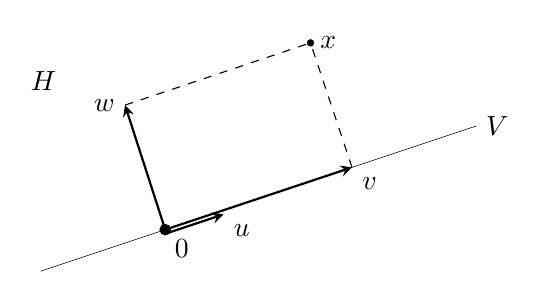
\begin{tikzpicture}[x=0.75pt,y=0.75pt,yscale=-1,xscale=1]
		\coordinate[label=below right:$0$] (O) at (200,190);

		\draw [very thin] (140,210) -- (350,140) node [right] {$V$};
		\draw (134,112.4) node [anchor=north west][inner sep=0.75pt] {$H$};

		\draw [fill=black] (O) circle (2.5);

		\draw [thick, -stealth] (O) -- (180.63,130) node [left] {$w$};
		\draw [thick, -stealth] (200,192) -- (228.1,182.63) node [below right] {$u$};
		\draw [thick, -stealth] (O) -- (290,160) node [below right] {$v$};

		\draw[fill=black] (270,100) circle (1.5) node[right] {$x$};
		\draw [dashed, thin] (290,160) -- (270,100);
		\draw [dashed, thin] (180.63,130) -- (270,100);
		\end{tikzpicture}
		\caption{Geometric intuition behind the proof of the projection theorem.}
	\end{figure}
	\FloatBarrier
	Then we have:
	\begin{align*}
		\inf_{y \in V} \norm{x-y}^2 &= \norm{w}^2\\
		&\leq \norm{x-\underbrace{(v+\lambda u)}_{\in V}}^2\\
		&= \norm{w- \lambda u}^2\\
		& = \norm{w}^2-2\lambda\sca{w,u} + \lambda^2 \norm{u}^2.
	\end{align*}
	Then we have $-2 \lambda \sca{w, u} + \lambda^2 \norm{u}^2 \geq 0$, thus $\lambda^2 \norm{u}^2 \geq 2 \lambda \sca{w,n}$ which implies 
	$$
		|\sca{w, u}| < \frac{|\lambda|}{2}\norm{u}^2.
	$$
	Letting $\lambda$ go to zero, we get:
	$$\sca{w,n} = 0 \quad \forall u \in V.$$
	Thus we have proven that $x=v+w$ where $w\in W=V^{\perp}$.\\
	We are left to prove that $V=W^{\perp}$ so that $H=V\oplus V^{\perp}$.\\
	Observe that $V\subset W^{\perp}$.\\
	On the other hand if $x\in W^{\perp}$ then:
	$$
		x=u^{\star} +w^{\star} ,\ \ u^{\star} \in V,w^{\star} \in W.
	$$
	Thus $x-u^{\star} \in W\cap W^{\perp} =\{0\}$ and this gives $x=u^{\star}$ so that $x\in V$.
\end{proof}
On account of this theorem we can give the following definition.

\begin{defn}[orthogonal projectors]
	Let $(H, \sca{\cdot, \cdot})$ be a Hilbert space, and $V \subset H$ be a closed subspace.\\
	Let also $v$ the unique element of $V$ such that $\norm{x-v} = d(x, V)$.\\
	Define the following \emph{projector} of $H$ onto $V$:
	$$P_V : H \to V  \quad P_V x = v.$$
	In the same way we can define the projector of $H$ onto $V^\perp$:
	$$P_{V^\perp}: H \to V^\perp \quad P_{V^\perp} x = x-v = x - P_V x.$$
\end{defn}
Notice that $x = P_V x + P_{V^\perp} x$.

$P_V$ is linear and bounded, namely: $$P_V \in \Bc(H, H).$$

\begin{itemize}
\item boundedness is easy:
$$
	\norm{x}^2 =\Vert P_V x\Vert^2 +\norm{P_{V^{\perp}} x}^2 \ \ \implies  \ \ \norm{P_V x} \leq \norm{x} 
$$
\item linearity is a bit harder:
$$
	\begin{drcases}
	\alpha x-P_V( \alpha x) \in V^{\perp}\\
	\alpha x-\alpha P_V(x) \in V^{\perp}
	\end{drcases}
	\implies \cancel{\alpha x}-P_V( \alpha x) -[\cancel{\alpha x} -\alpha P_V(x)] \in V^{\perp}
$$
but also
$$
	\alpha \underbrace{P_V(x)}_{\in V} -\underbrace{P_V( \alpha x)}_{\in V} \in V
$$
thus
$$
	\alpha P_V(x) -P_V( \alpha x) \in V^{\perp} \cap V=\{0\} \ \ \implies  \ \ \alpha P_V(x) =P_V( \alpha x)
$$
A similar argument can be done to prove that $P_V(x) +P_V(y) =P_V(x+y)$.
\end{itemize}

%\begin{rema} % Possible repetition?
%	Let $(H, \sca{\cdot, \cdot})$ be a Hilbert space, and $V \subset H$ be a closed subspace. \\
%	Then $(V^\perp)^\perp = V$, and $V^\perp = \{0\}$ if and only if $V=H$. \\
%	Notice that, if $V$ is not closed, $V^\perp = \{0\}$ if and only if $\widebar V = H$.
%\end{rema}

%!TEX root = ../main.tex
\subsubsection{Dual of a Hilbert Space and Riesz's representation theorem} \todo{accorpare al precedente?}
In this chapter we will introduce a theorem which play an important role in application.\\
Start with an observation. Consider a Hilbert Space, namely $(H, \sca{\cdot, \cdot})$ and fix one of his elements $y \in H$. Define the operator $L_y$ as follows:
$$|L_yx| = |\sca{y,x} | \quad \forall x \in H.$$
Then this operator belongs to the dual of $H$ and we will write $L_y \in H$. As $|L_yx| = |\sca{y,x} | \leq \norm{y} \norm{x}$, we have that $\norm{L_y}_{H^\star} \leq \norm{y}$: with the fact that $H$ is reflexive this implies that $\norm{L_y}_\star = \norm{y}$.\\
Now we have to acknowledge that there exists an isometry $J : H \to H^\star, \ y \mapsto L_y = \sca{x, y}$.

This reasoning can be revert: the converse is also true and we have

\begin{theo}[Riesz's representation theorem] \label{riesz-repr}
	Let $(H, \sca{\cdot, \cdot})$ be a Hilbert space.\\
	An operator $L \in H^\star$ if and only if there exists a unique $y \in H$ such that $Lx = \sca{y, x}$ for all $x \in H$.
	%$J: H \to H^\star$ is surjective. In other words:
	%$$\forall L \in H^\star \quad \exists ! \, y \in H : \enspace Lx = \sca{y, x} \quad \forall x \in H$$
\end{theo}
In other words, $J: H \to H^\star$ is surjective.\\

Observe that the reflexivity of $H$ can be proven using this theorem.\\
Note also that as $n \to \infty$ we have $$\sca{x_n,y} \to \sca{x,y} \ \forall y \in H \text{ if and only if }x_n \wto x.$$

We will prove the ``only if'' part as the ``if'' part can be deduced from the introduction. \todo{a better organization is more suitable for a book}

\begin{proof}\textit{Proof of the necessary condition $\impliedby$.}\\
	If $L \equiv 0$, then we choose $y=0$ and the thesis is obtained.\\
	\textit{General case.}\\	
	Consider $L \not \equiv 0$. Then $\Ker(L)$ is a closed proper subspace of $H$, that is $\{0\} \subsetneq \Ker(L)^\perp$.\\
	Then, applying the projection theorem and then normalizing, we can find $z \in \Ker(L)^\perp$ such that $\norm{z}=1$; then for any $x \in H$  since:
	$$L\left( x-\frac{Lx}{Lz}z \right)
	= Lx - \frac{Lx}{Lz} Lz =0,$$
	we have
	$$x- \frac{Lx}{Lz} z
	\in \Ker(L).$$
	
	Thus:
	$$\sca{x - \frac{Lx}{Lz}z, z} = 0,$$
	which implies 
	$$\sca{x, z} = \sca{\frac{Lx}{Lz}z,z} = \frac{Lx}{Lz} \text{ and } Lx = \sca{x, (Lz)z} \quad \forall x \in H.$$ 
	We choose $y =  (Lz)z \in Y$.
	
	\textit{The element $y$ is unique.}\\
	If $Lx = \sca{y_1, x} = \sca{y_2, x}$ for all $x \in H$, then $ \sca{y_1-y_2, x} = 0$ $\forall x \in H$.\\
	Choosing $x = y_1 - y_2$, we have $\norm{y_1-y_2}^2=0$, and finally $y_1 = y_2$.
\end{proof}

We can say that $H$ and $H^\star$ is linearly and isometrically isomorphic, through the linear isometry and isomorphism we introduced before $J$. This isomorphism is called \emph{Riesz map}. It can be defined also as $J: H^\star \to H$ by setting
$$JL = y \text{ where } Lx = \sca{x, JL} \ \forall x \in H.$$
As it is a linear bijection and an isometric isomorphism we have $\norm{JL} = \norm{L}_\star$.


\begin{prop}
	Consider the following inner product on $H^\star$:
	$$\sca{L_1, L_2}_\star \coloneqq \sca{J^{-1}L_1, J^{-1} L_2} \quad \forall L_1, L_2 \in H^\star.$$
	Then $(H^\star, \sca{\cdot, \cdot}_\star)$ is a Hilbert space.
\end{prop}

The induced norm is the existing norm in $H^\star$:
$$\sca{L_1, L_2}_\star = \norm{JL_1}^2 = \norm{L_1}^2_\star$$
because  $\norm{L_1}_\star =
\sqrt{\sca{L_1, L_1}_\star \vphantom{\tilde L}} =
\sqrt{\sca{J^{-1}L_1, J^{-1} L_2} } 
= \norm{J^{-1} L_1} = \norm{L_1}_{H^\star}$.

Taking advantage of the Riesz's representation theorem you can prove that any Hilbert space is reflexive: this is  a really though exercise.

%!TEX root = ../main.tex
\subsubsection{Proof of the Radon--Nikodym Theorem} \label{proof-radon-nikodym}
The theorem is named after Johann Radon, who proved the theorem for the special case where the underlying space is $\RR^{N}$ in 1913, and after Otto Nikodym who proved the general case in 1930. It is a representation theorem: it provides, under suitable assumptions, a link between two measures.

The theorem is explained in \vref{derivative-of-a-measure}, for a better use of this book we copy-pasted it here.  
\begin{theo} [Radon--Nikodym]
	Let $(\Omega, \mm,\mu)$ be a complete measure space, and $\nu$, $\mu$ two measures on $(\Omega, \mm)$.\\
	If $\mu$ is $\sigma$-finite and $\nu\ll\mu$, then the Radon--Nikodym derivative $\frac{\de\nu}{\de\mu}$ exists.
\end{theo} 

This proof belongs to John von Neumann (1903--1957).

\begin{proof}
	
	\textit{Set up:}\\
	For simplicity we consider the w
	Consider $\mu, \nu$ finite, namely $\mu(\Omega), \nu(\Omega) < \infty$), such that $\nu \ll \mu$.\\
	Let $\lambda = \mu + \nu$. Then, for every non-negative and measurable function $f$ we have the \emph{additivity with respect to measure}:
	$$\int_\Omega f \dlam = \int_\Omega f \dmu + \int_\Omega f \dnu$$
	which is a direct consequence of the definition of Lebesgue interval.
	
	\textit{First step, use of the Hölder inequality and the Riesz's representation theorem:}\\
	Suppose $f \in L^2_\lambda(\Omega)$. Applying the Hölder inequality we have:
	\begin{align*}
	\abs{\int_\Omega f \, \dnu}
	&\leq \int_\Omega |f| \, \dnu\\
	&\leq \int_\Omega |f| \, \dlam\\
	&\leq \left( \int_\Omega |f|^2 \, \dlam \right)^{\frac 1 2}(\lambda(\Omega))^\frac{1}{2}\\
	&= \norm{f}_{L^2_\lambda (\Omega)}(\lambda(\Omega))^\frac{1}{2}\\
	&< +\infty
	.
	\end{align*}
	Thus $F: f \mapsto \int_\Omega f \dnu$ is a linear bounded functional on $L^2_\lambda(\Omega)$, from which we deduce:
	$$\norm{F}_{(L^2_\lambda (\Omega))^\star} \leq (\lambda(\Omega))^\frac{1}{2}.$$
	
	Applying Riesz's representation theorem (\vref{riesz-repr}) there exists $g \in L^2_\lambda(\Omega)$ such that:
	$$ F(f) = \int_\Omega f \,\dnu = \int_\Omega f g \, \dlam \quad \forall f \in L^2_\lambda(\Omega).$$
	
	For any $E \in \mm$ such that $\lambda(E) > 0$, consider $f = \Ind_E$; we have:
	$$ 0 
	\leq \nu(E) 
	= \int_\Omega f \,\dnu 
	= \int_\Omega f g \, \dlam 
	= \int_E g \, \dlam
	= F(\Ind_E)
	\leq \lambda(E)
	.
	$$
	So $\nu(E) \leq \lambda(E)$ and then:
	$$0 \leq \frac{1}{\lambda(E)} \int_E g \, \dx \leq 1.$$
	
	\textit{Second step:}\\
	As $E$ is arbitrary we have $ 0 \leq g(x) \leq 1$ almost everywhere with respect to the measure $\lambda$, and thus with respect to $\nu$ and $\mu$.\\
	We can suppose that there exists $\tilde \Omega \in \mm$ such that $0 \leq g(x) \leq 1$  for any $x \in \tilde\Omega$.\\
	So $\lambda(\tilde\Omega\comp) = 0$, and we define $g(x) = 1$ for all $x \in \tilde\Omega\comp$.
	
	Then, for any $f \in L^2_\lambda(\Omega)$:
	$$
	\int_\Omega f \,\dnu 
	= \int_\Omega f g \, \dlam 
	= \int_\Omega f g \, \dmu + \int_\Omega f g \, \dnu
	$$
	and we can rewrite in this way:
	$$
	\int_\Omega (1-g)f \, \dnu 
	= \int_\Omega f g \, \dmu.
	$$
	
	\textit{Third step, convergences:}\\
	Let $A = \{x \in \Omega : \ 0 \leq g(x) < 1 \}$, and $B = A\comp$.\\
	Taking $f= \Ind_B$ in the previous identity we find $\mu(B)=0$.\\
	By hypothesis $\nu \ll \mu$, and thus $\nu(B) = 0$.
	
	Define $$\Phi_n = \sum_{j=0}^{n+1} g^j.$$
	
	Take now $f=(1+g+g^2+\cdots+g^n)\Ind_E$ in the same identity, with $E \in \mm$, $n \in \NN$. We get:
	$$
	\int_E(1-g^{n-1}) \,\dnu 
	= \int_E\Phi_n \,\dmu
	.
	$$
		
	Observe that as $n \to +\infty$ and $0 \leq 1-g^{n+1} \leq 1$ in $\Omega$ we have $1-g^{n+1} \to 1$ almost everywhere with respect to $\nu$ and, due to $\nu (B) = 0$:
	$$\int_E(1-g^{n-1}) \,\dnu
	= \int_{E \cap A}(1-g^{n-1}) \,\dnu
	+ \underbrace{\int_{E \cap B}(1-g^{n-1}) \,\dnu}_{= 0 \ \forall n}
	\ \to \ \nu(E \cap A) 
	= \nu(E)
	.
	$$
	
	First, applying dominate convergence theorem which entails:
	$$
	\lim\limits_{n \to \infty} \int_E (1+g^{n+1}) \, \dnu 
	= \nu(E)
	.
	$$
	
	Second, as $\Phi_n \uparrow \Phi$ monotonically and $\Phi = \lim_n \Phi_n$ is measurable, we can use monotone convergence theorem and obtain:
	$$
	\int_E \Phi_n \dmu 
	\to \int_E \Phi \dmu
	.
	$$
	
	Thus we can conclude deducing:
	$$
	\nu(E) 
	= \int_E \Phi \dmu 
	\quad \forall E \in \mm
	.
	$$
	
	Note also that $\Phi$ is measurable and belongs to $L^1_\mu(\Omega)$ as $\nu$ and $\mu$ are finite.
\end{proof}

%!TEX root = ../main.tex
\subsubsection{Bilinear Forms and Lax Milgram lemma}
Here we will generalize the concept of inner product. In fact, the following definition will make it clear that the inner product is an operation which belongs to a much general class.

\begin{defn}
	Let $(H, \sca{\cdot, \cdot})$ be a Hilbert space.\\
	An application $a: \, H \times H \to \RR$ is called \emph{bilinear form} if:
	\begin{align*}
		u &\mapsto a(u,v) \text{ is linear for each fixed } v \in H,\\
		v &\mapsto a(u,v) \text{ is linear for each fixed } u \in H.
	\end{align*}
\end{defn}

\begin{defn}
	A bilinear form $a: \, H \times H \to \RR$ is \emph{coercive} if there exists $\alpha > 0$ such that:
	$$a(u,u) \geq \alpha\norm{u}^2 \quad \forall u \in H.$$
\end{defn}

\begin{prop}
	A bilinear form $a: \, H \times H \to \RR$ is continuous if and only if there exists $M > 0$ such that:
	$$ \abs{a(u,v)} \leq M\norm{u}\norm{v} \quad \forall u, v \in H.$$
\end{prop}

Observe that the inner product of an Hilbert space is a continuous and coercive bilinear form.

Consider $H = \RR^N$ with the euclidean scalar product $\sca{\cdot, \cdot}_2$ and a matrix $A \in \RR^{N \times N}$.
Then $a(x,y) = \sca{Ax, y}_2$ for all $x, y \in \RR^N$ is a continuous bilinear form.

The following is a lemma which generalize the last representation theorem.

\begin{theo}[Lax--Milgram]\label{theo-lax-milgram}
	Let $a:\, H \times H \to \RR$ be a continuous and coercive bilinear form.\\
	Then for any $l \in H^\star$ there exists a unique $u \in H$ such that:
	$$a(u,v) = Lv \quad \forall v \in H.$$
	Moreover we have
	$$\norm{u} \leq \frac{1}{\alpha}\norm{L}_\star$$
	where $\alpha$ is the coercivity constant.
\end{theo}

\begin{proof}
	Fix $u \in H$ and observe that:
	$$
		v \in H:\
		v \mapsto a(u,v) \in \RR
	$$
	is an element of $H^\star$.
	Therefore there is a unique $h \in H$ such that:
	$$
		a(u,v) 
		= \sca{h,v} 
		\quad \forall v \in H
		.
	$$
	Thus we can define a linear operator $A:H \to H$ by setting $Au = h$. This operator is also bounded. Indeed:
	$$
		\norm{Au}^2 
		= \sca{Au, Au} 
		= a(u, Au) 
		\leq M \norm{u} \norm{Au}
	$$
	so that $\norm{Au} \leq M \norm{u}$.
	
	Moreover, we have:
	$$
		\alpha\norm{u}^2 
		\leq a(u,u) 
		= \sca{Au, u} 
		\leq \norm{Au}\norm{u}
	$$
	so $A$ is also injective.
	
	On the other hand, there is a unique $w \in H$ such that (see Riesz's representation theorem \vref{riesz-repr}):
	$$
		Lv 
		= \sca{w, v} 
		\quad \forall v \in V
		.
	$$
	Therefore the thesis can be reformulated as follows: for any $w \in H$ find a unique $u \in H$ such that:
	$$
		\sca{Au, v} 
		= \sca{w,v} 
		\quad \forall v \, \in V
	$$
	so we're left to show that $A$ is surjective.
	
	Let's prove first that $\Im(A)$ is a closed subspace of $H$.\\
	Indeed let $\{y_n\}_{n\in \NN} \subset \Im(A)$ be such that $y_n \to y$ as $n \to \infty$.\\
	We know that there exists a unique $u_n \in H$ such that $A u_n = y_n$.\\
	Moreover, we have
	$$
		\alpha \norm{u_n - u_m} 
		\leq \norm{A u_n - A u_m} 
		= \norm{y_n - y_m}
	$$
	therefore $\{u_n\}_{n \in \NN}$ converges in $H$ to some $u$ and, because $A$ is continuous, it follows
	$$
		A u_n 
		\to A u 
		\quad n \to \infty
		.
	$$
	Hence $y=Au \in \Im(A)$ and $\Im(A)$ is closed.
	
	We can now prove that $A$ is surjective.\\
	By contradiction suppose that $\Im(A) \subsetneq H$. Then there exists $y_0 \in H$ such that $y_0 \neq 0$ and $y_0 \in \Im(A)^\perp$. However, we have
	$$
		0 
		= \sca{A y_0, y_0} = a(y_0,y_0) 
		\geq \alpha\norm{y_0}^2 
		\implies y_0 = 0
		.
	$$
	This is a contradiction.
	
	Finally, we recall that
	$$
		\alpha\norm{u} 
		\leq \norm{Au} 
		= \norm{w} 
		= \norm{L}_\star
		.
	$$
\end{proof}

\paragraph{Inner product} Even if a scalar product is a continuous and coercive bilinear form, a continuous and coercive bilinear form is not necessarily a scalar product: this because it might be not symmetric.\\
Due to this point, the Lax--Milgram lemma can be seen as a generalization of the Riesz representation theorem (\vref{theo-projection}).

\begin{prop}
	Let $a: \, H \times H \to \RR$ be a continuous and coercive bilinear form.\\
	If $a$ is symmetric, namely:
	$$
		a(u,v) 
		= a(v,u) 
		\quad \forall u,v \in H
		.
	$$
	then $a$ is a scalar product in $H$ and its induced norm is equivalent to the norm in $H$.
\end{prop}

\begin{proof}
	By coercivity and the other hypothesis we have:
	$$
		\alpha \norm{u}^2 
		\leq a(u,u) \leq M\norm{u}^2 
		\quad \forall u \in H
	$$
	where $\norm{\cdot}$ is the norm in $H$.\\
	
	Hence $a(u,u) \geq 0$ for all $u \in H$ and $a(u,u) = 0$ if and only if $u = 0$.
	
	Thus $a(\cdot, \cdot)$ is a scalar product in $H$ and its induced norm
	$$
		\norm{u}_a 
		= \sqrt{a(u,u)}
	$$
	is equivalent to $\norm{\cdot}$.
\end{proof}


\paragraph{An application of the Lax--Milgram lemma}\label{app-lax-milgram} All this theory has a practical purpose. Here we will see in action the tools we built solving a differential problem.\\
Consider the following boundary value problem: find $u$ such that
$$
	\begin{cases}
	-(  \alpha(x) u' + \beta(x) u)' + \gamma(x)u 
	= f(x)
	\quad x \in (a,b)\\
	u(a) 
	= u(b) 
	= 0
	\end{cases}
$$
where $\alpha, \beta \in \Cc^1([a,b])$ and $\gamma, f \in C([a,b])$.

Suppose $w \in \Cc^2([a,b])$ is a classical solution to the problem.

Consider $\phi \in \Cc^\infty((a,b))$ multiply the equation by $\phi$ and integrate over $(a,b)$.
Integrating by parts we get the identity:
$$
	\int_a^b \left[
	\left(\alpha(x)w'(x)
	+ \beta(x)w(x) \right)\phi'(x)
	+ \gamma(x)w(x)\phi(x)\right]\,\dx 
	= \int_a^bf(x) \phi(x) \, \dx
	.
$$

Setting
$$
	V_0
	= \{v \in H^1((a,b))
	: \ v(a)
	=v(b)
	=0\}
$$
where $H^1((a,b)) = W^{1,2}((a,b))$, we observe that $V_0$ is a closed subspace of $H^1((a,b))$. Moreover the scalar product
$$
	(v_1, v_2) 
	= \int_a^b v_1'(x) v_2'(x) \, \dx
$$
induces a norm
$$
	\norm{v}_0 
	= \norm{v'}_2
$$
which is equivalent to the standard norm in $H^1((a,b))$.\\
(This because the Poincaré's inequality $\norm{v}_2 \leq (b-a)\norm{v'}_2$.)\\

We can prove that $C_C^\infty((a,b))$ is dense in $V_0$ (this is a density theorem: density theorems allow to establish approximations) which allows us to deduce that our solution $w$ satisfies the identity
$$ 
	\int_a^b [(\alpha(x)w'(x) + \beta(x)w(x))v'(x) + \gamma(x)w(x)v(x)]\,\dx = \int_a^bf(x) v(x) \, \dx \quad \forall v \in V_0. 
$$

We can now look at our problem from a more general standpoint.

Let us set, for all $u,v \in V_0$
$$
	a(u,v)
	= \int_a^b [(\alpha(x)u'(x) 
	+ \beta(x)u(x))v'(x) 
	+ \gamma(x)u(x)v(x)]\,\dx
$$
and observe that $a: \, V_0 \times V_0 \to \RR$ is a bilinear form.

Thus we can give to the original problem a weaker formulation, namely find $w \in V_0$ such that
$$
	a(w,v)
	=Lv
	\quad \forall v \in V_0
$$
where $L \in V^\star_0$ is defined by 
$$
	Lv 
	= \int_a^b f(x)v(x)\, \dx 
	\quad \forall v \in V_0
	.
$$

Now we want to apply Lax--Milgram lemma. Let's check the hypothesis.

Observe that $a(\cdot, \cdot)$ is continuous as 
\begin{align*}
	\abs{a(u,v)} 
	&\leq \int_a^b \abs{(\alpha(x)u'(x) 
	+ \beta(x)u(x))v'(x) 
	+ \gamma(x)u(x)v(x)}\,\dx\\
	&\leq \norm{\alpha}_\infty \int_a^b \abs{u'v'}\,\dx
	+\norm{\beta}_\infty \int_a^b \abs{uv'}\,\dx
	+\norm{\gamma}_\infty \int_a^b \abs{uv}\,\dx\\
	&\leq \norm{\alpha}_\infty \norm{u'}_2 \norm{v'}_2
	+ \norm{\beta}_\infty \norm{u}_2 \norm{v'}_2
	+ \norm{\gamma}_\infty \norm{u}_2 \norm{v}_2
\end{align*}

for all $u,v \in V_0$.\\
Then, using again the Poincaré's inequality we have:
$$
	\abs{a(u,v)}\leq \norm{\alpha}_\infty \norm{u'}_2 \norm{v'}_2
	+ (b-a)\norm{\beta}_\infty \norm{u'}_2 \norm{v'}_2
	+ (b-a)^2 \norm{\gamma}_\infty \norm{u'}_2 \norm{v'}_2
	.
$$

Hence, setting 
$$
	M = \norm{\alpha}_\infty
	+ (b-a)\norm{\beta}_\infty
	+ (b-a)^2\norm{\gamma}_\infty
	,
$$
we have
$$
	\abs{a(u,b)} 
	\leq M \norm{u}_0\norm{v}_0 
	\quad \forall u, v \in V_0
	.
$$

We can add other assumption to the coefficients $\alpha$, $\beta$ and $\gamma$ that hold for any $x \in [a,b]$, like the following:
$$
	\alpha_0
	= \min\limits_{x\in[a,b]} \alpha(x)
	> (b-a) \norm{b}_\infty
	\text{ and }
	\gamma(x) 
	\geq 0
	.
$$

Collecting the results we obtained we have:
\begin{align*}
	a(u,u)
	&= \int_a^b \alpha(x)(u'(x))^2 \, \dx
	+ \int_a^b \beta(x)u(x)u'(x) \, \dx
	+ \int_a^b \gamma(x)(u(x))^2 \, \dx \\
	& \geq \alpha_0\norm{u'}_2
	+ \int_a^b \beta(x)u(x)u'(x) \, \dx.
\end{align*}

We can find an upper bound for the middle term as well:
$$
	\abs{\int_a^b \beta(x)u(x)u'(x) \, \dx}
	\leq \norm{\beta}_\infty \norm{u}_2 \norm{u'}_2 
	\leq (b-a) \norm{\beta}_\infty \norm{u'}_2^2
	,
	$$
	so we get:
	$$
	a(u,u)
	\geq [\alpha_0 -(b-a)\norm{\beta}_\infty] \, \norm{u'}_2
	$$
	we can set:
	$$
	\alpha 
	= [\alpha_0 -(b-a)\norm{\beta}_\infty]
	> 0
	.
$$

Then, finally we have:
$$
	a(u,u)
	\geq \alpha \norm{u}_0
	.
$$
and we can conclude that $a(\cdot, \cdot)$ is coercive.

Now we can apply the Lax--Milgram lemma and we deduce the following proposition:
If $\alpha$, $\beta$, $\gamma$, $f \in C([a,b])$ and 
$$
	\min\limits_{x\in[a,b]} \alpha(x)
	> (b-a) \norm{b}_\infty
	\text{ and }
	\gamma(x) 
	\geq 0
	\quad \forall x \in [a,b]
	$$
	then there exists a unique $u \in V_0$ such that:
	$$
	a(u,v) 
	= Lv \quad \forall v \in V_0
	.
$$

The solution $u$ given by the Lax--Milgram lemma is a weak solution to the original boundary value problem.

We can further weaken the assumptions on the coefficients by taking $\alpha$, $\beta$, $\gamma \in L^\infty((a,b))$.

In addiction $f$ can be taken in $V_o^\star$: assume $f \in L^2((a,b))$ or even a linear bounded functional link, for instance,
$$
	Lv
	= v(x_0)
	\quad \forall v \in V_0
$$
where $x_0 \in (a,b)$. It's easy to check that $L \in V_0^\star$.

Consider now the linear application $K:L^2((a,b)) \to L^2((a,b))$
defined by
$K:f\mapsto u$
where $u$ satisfies
$$
	a(u,v) 
	= \int_a^b fv 
	\quad \forall v \in V_0
	.
$$

We have that $\Im(K) \subseteq V_0$ and we know that 
$$
	V_0
	\hookrightarrow \hookrightarrow C([a,b])
	\hookrightarrow L^2((a,b))
	.
$$

Therefore
$$
	V_0
	\hookrightarrow \hookrightarrow L^2((a,b))
	.
$$
Hence $K$ is a compact operator.

From Lax--Milgram we have also a stability estimate:
$$
	\norm{u}_0
	\leq \frac 1 \alpha \norm{L}_{V_0^\star}
	.
$$

If $f \in L^2((a,b))$ then, using Poincaré's inequality:
$$
	\abs{Lv}
	= \abs{\int_a^b f v \, \dx}
	\leq \norm{f}_2\norm{v}_2
	\leq (b-a)\norm{f}_2\norm{v}_0
$$
so that
$$
	\norm{L}_\star
	\leq (b-a)\norm{f}_2
$$
and
$$
	\norm{u}_0
	\leq \frac{(b-a)}{\alpha} \norm{f}_2
	.
$$

If
$$Lv 
	= v(x_0) 
	\quad \forall v \in V_0
$$

where $x_0 \in (a,b)$, then, using Hölder's inequality:
$$
	\abs{Lv}
	= \abs{v(x_0)}
	= \abs{\int_a^{x_0} v'(y) \, \dy}
	\leq (b-a)^{(\frac 1 2)} \norm{v}_0
$$

so that
$$
	\norm{L}_\star
	\leq (b-a)^{\frac 1 2}
$$
and
$$
	\norm{u}_0
	\leq
	\frac{(b-a)^{\frac 1 2}}{\alpha}
	.
$$

The bilinear form $a(\cdot, \cdot)$ is not symmetric because of $\beta$.\\
If $\beta \equiv 0$ then we deal with following boundary value problem
$$
	\begin{cases}
	-(\alpha(x)u')' 
	+ \gamma(x)u 
	= f(x) 
	\quad x \in (a,b)\\
	u(a) 
	= u(b) 
	= 0
	\end{cases}
$$
and its weak formulation has a unique solution provided that, for instance
$$
	\alpha = \min_{x\in [a,b]} \alpha (x) > 0
	, 
	\quad \gamma(x)\geq 0 
	\quad x \in [a,b]
	.
$$
However, in this case we can just apply the Riesz representation theorem since $a(\cdot, \cdot)$ is an inner product in $V_0$ whose induced norm is equivalent to $\norm{\cdot}_0$.

%!TEX root = ../main.tex
\subsubsection{Bases in Hilbert spaces}
In this section we will see that elements of Hilbert spaces can be represented with respect to a series of vectors, known as basis. The idea is the same of Linear Algebra, but now we are dealing with infinite dimensional spaces, thus things require a higher level of technicality and not every operation can be done without some specific assumptions.

\begin{defn}
	Let $(H, \sca{\cdot,\cdot})$ be a Hilbert spaces.\\
	A set of orthogonal vectors $E \subset H$ is \emph{complete} if, given a vector $x \in H$ such that $\sca{x, u} = 0$ for all $u \in E$, then $x = 0$.
	%$$x \in H : \enspace \sca{x, u} = 0 \enspace \forall u \in E \implies x = 0$$
	
	A subset is an \emph{orthogonal basis} if $E$ consists of orthogonal vectors and is complete.\\		
	An orthonormal basis whose vectors have unitary norm (an then consists of orthonormal vectors) is an \emph{orthonormal basis}.
\end{defn}

% If $E$ is complete, then $E^\perp = \{0\}$, hence $\sca{E} ^ \perp= \sca{0}$, and finally $\widebar{\sca{E}}= \{ 0\}$. \\
% Remember that $\sca{E}$ denotes the vector space generated by $E$. \todo{check if this is specified somewhere}

If $E$ is an orthonormal basis of $H$ then $\widebar{\mathrm{span}E}^\perp = E^\perp = \{0\}$. Thus $\widebar{\mathrm{span}E} = H$. \\
One can prove that, if $H$ is separable, a countable orthogonal basis is a Schauder basis.
\begin{theo}
	If a Hilbert space contains at least two distinct vectors, then it has an orthonormal basis.
\end{theo}
We are going to prove the theorem in a constructive way, using Gram--Schmidt orthogonalization, supposing $H$ separable.\\
If $H$ is non-separable,\footnote{``Non-separable Hilbert spaces are quite exotic.'' - M. G.} then the proof requires Zorn's Lemma.
\begin{proof} %not checked
	Let $\{v_n\}_{n \in \NN} \subset H$ be a dense set.\\
	Set 
	$$F_h = \sca{v_1, \ldots, v_h} \quad \forall h \in \NN_0.$$
	Observe that for all $h \in \NN_0$, $F_h$ is a closed subspace of $H$ and $F_h \subset F_{h-1}$.
	
	Take $v_1 \in V_1$ and set 
	$$e_1 = \frac{v_1}{\norm{v_1}}.$$
	In $V_2 \supsetneq V_1$, thanks to the projection theorem, we can find $e_2 \in V_1^\perp$ such that $\norm{e_2} = 1$.\\
	Therefore $\{e_1, e_2\}$ is an orthonormal basis in $V_2$.\\
	Then we proceed by induction, getting an orthonormal basis of $H$.
\end{proof}

\begin{theo}
	All the orthonormal basis in a Hilbert space  have the same cardinality.
\end{theo}
\begin{defn}
	The cardinality of an orthonormal basis of an Hilbert space $(H, \sca{\cdot,\cdot})$ is called \emph{orthogonal dimension} of $H$, and is denoted by $\dim_\perp H$.
\end{defn}
If $H$ is also separable, then $\dim_\perp H \leq \aleph_0$. Indeed, if $u, v \in D$, $u \neq v$, then $\norm{u-v}^2 = \norm{u}^2 +\norm{v}^2 = 2 > 0$. So if $\dim_\perp H \leq \aleph_0$ we cannot find a countable dense set. 


\begin{exam}
	Let $H=l^2$, with $\sca{x, y} = \sum_{i \in \NN} x_i y_i$.\\
	Define the set of sequences $\{\vec e^j\}_{j \in \NN}$ as follows:	
	$$
	e_i^j
	=\begin{cases}
	1 
	& \text{if } i=j \\ 
	0
	& \text{if } i \neq j.
	\end{cases}
	$$
	Then $\{\vec e_j\}_{j \in \NN}$ is an orthonormal basis of $l^2$ and we have:
	$$
	x
	=\sum_{j \in \NN} x_j \vec e^j
	\quad \forall x = \{x_n\}_{n \in \NN} \in l^2.$$
\end{exam}

\begin{exam}
	If $H = L^2((-\pi, \pi))$
	then we can prove that
	$$
		\left\{
			\frac{1}{\sqrt{2\pi}}, 
			\frac{\sin(nt)}{\sqrt \pi}, 
			\frac{\cos(nt)}{\sqrt \pi}
		\right\}_{n \in \NN_0}
	$$
	is an orthonormal basis in $H$. 
\end{exam}

\paragraph{Fourier basis} Now we will use the tools we developed to introduce the Fourier series, which allows to represent continuous function in a different way. In particular, Fourier series is a very powerful tool in engineering since it helps breaking down almost any kind of function in a sum of smooth pieces, which are much easier to treat. This is also very useful when solving partial differential equations for the same reason.

\begin{theo}[Bessel's inequality]
	Let $\{u_n\}_{n \in \NN}$ be a set of orthonormal vectors in $H$.\\
	Then, for all $x \in H$, we have
	$$\sum_{n\in\NN} |\sca{x, u_n}|^2 \leq \norm{x}^2$$
\end{theo}

\begin{proof}
	The absolute value is only really needed when the field is $\CC$, while in this treaty we only used $\RR$. We will however provide a complete proof for the sake of understanding where each term comes from. The reader may revise some concepts, like conjugate in complex numbers, before reading the proof.
	\begin{align*}
	0 & \leq \norm{x-\sum\limits_{n=0}^k \sca{x,u_n} u_n}^2\\
	 & =\sca{x-\sum\limits_{n=0}^k \sca{x,u_n} u_n ,x-\sum\limits_{n=0}^k \sca{x,u_n} u_n} \\
	 & =\sca{x,x} -2\underbrace{\sca{x,\sum\limits_{n=0}^k \sca{x,u_n} u_n}}_{( *)} +\underbrace{\sca{ \sum\limits_{n=0}^k \sca{x,u_n} u_n ,\sum\limits_{n=0}^k \sca{x,u_n} u_n}}_{( **)} =( ***)
	\end{align*}
	The second term becomes
	\begin{align*}
	( *) & =\sum\limits_{n=0}^k \sca{x,\sca{x,u_n} u_n}  & \text{(sesquilinearity)}\\
	 & =\sum\limits_{n=0}^k\overline{\sca{ \sca{x,u_n} x,u_n}} =\sum\limits_{n=0}^k\overline{\sca{x,u_n} \sca{x,u_n}} & \text{(conjugate symmetry)}\\
	 & =\sum\limits_{n=0}^k \sca{ u_n ,x} \overline{\sca{x,u_n}} & \text{(conjugate)}\\
	 & =\sum\limits_{n=0}^k| \sca{x,u_n} |^2 & \text{(conjugate product)}
	\end{align*}
	While the third
	\begin{align*}
	( **) & =\norm{ \sum\limits_{n=0}^k \sca{x,u_n} u_n}^2 \leq \sum\limits_{n=0}^k| \sca{x,u_n} |^2\underbrace{\norm{u_n}^2}_{=1}
	\end{align*}
	Thus
	$$
		(***) \leq \norm{x}^2 -\sum\limits_{n=0}^k| \sca{x,u_n} |^2
	$$
	Letting $k$ to infinity we get the thesis.
\end{proof}


\begin{defn}
	Let $(H, \sca{\cdot, \cdot} )$ be a separable Hilbert space and $\{u_n\}_{n \in \NN}$ one of its orthonormal basis.\\
	We define the \emph{Fourier coefficients} of $x \in H$ with respect to $\{u_n\}_{n \in \NN}$ as follows:
	$$x_n \coloneqq \sca{x, u_n}.$$
\end{defn}

\begin{theo}
	Let $(H, \sca{\cdot, \cdot} )$ be a separable Hilbert space and $\{u_n\}_{n \in \NN}$ one of its orthonormal basis.\\
	Then we can express any $x \in H$ with the following series:
	$$x=\sum_{n\in\NN} \sca{x, v_n} v_n.$$
	The series is known as \emph{Fourier series}.
\end{theo}
Observe that we can also write:
$$
	x = 
	\sum_{n \in \NN} x_n u_n
	\quad \forall x \in H
	\quad \text{ and } \quad
	\sca{x,y} =
	\sum_{n \in \NN} x_n y_n
	\quad \forall x,y \in H
	.
$$
\begin{proof}
	Observe that thanks to Bessel's inequality, $\sum_{n \in \NN} | \sca{x, v_n} |^2 = \sum_{n \in \NN} \abs{x_n}^2$ converges.\\
	Then the sequence of partial sums $S_n = \sum_{j=0}^n x_j vj$ is fundamental:
	$$
	S_n - S_m 
	= \norm{\sum_{j=m+1}^{n}\sca{x, v_j} v_j}^2 
	\leq \sum_{j=m+1}^n |\sca{x, v_j}|^2
	\to 0
	\text{ as } n \to \infty
	.
	$$
	
	Hence $\sum_{n \in \NN} x_n$ converges in $H$ to some $\tilde x$.\\
	Fix $m \in \NN$ for any $n > m$ we have:
	$$
	\sca{x - \sum_{j=0}^{n} x_jv_j, v_m} 
	= x_m - \sca{\sum_{j=0}^n x_j v_j, v_m}
	= x_m - x_m 
	= 0 
	.
	$$ 
%	\begin{align*}
%	\sca{x - \sum_{j=1}^N \sca{x, v_j} v_j, v_{n_0}}
%	&= \sca{x, v_{n_0}} 
%	- \sca{\sca{x, v_{n_0}} v_{n_0}, v_{n_0}} \\
%	&= \sca{x, v_{n_0}} 
%	- (\sca{x, v_{n_0}}) \sca{v_{n_0}, v_{n_0}}
%	= 0
%	\end{align*}
	Taking $n \to +\infty$, we have $\sca{x- \tilde x, v_{m}} = 0$ for all $m \in \NN$, and finally $x= \tilde x$ because $\{u_n\}_{n \in \NN}$ is complete.
\end{proof}

\begin{theo}[Parseval identity]
	Let $(H, \sca{\cdot, \cdot} )$ be a separable Hilbert space and $\{u_n\}_{n \in \NN}$ one of its orthonormal basis.\\
	Then we can write the inner product as the series of the products of the Fourier coefficients, namely:
	$$
	\sca{x, y} 
	= \sum_{n \in \NN}\sca{x, v_n} \sca{y, v_n}
	\quad \forall x, y \in H.
	$$
	This is known as \emph{Parseval identity}.
\end{theo}
\begin{proof}
 	Thanks to orthonormality, for any $n \in \NN$ fixed, we have:
	$$
	\sca{\sum_{j=1}^n x_j v_i, \sum_{j=1}^n x_j v_i}
	= \sum_{j=0}^n \sca{x, v_j} \sca{y, v_j}
	$$
	Letting $n \to +\infty$, the first term converges to $\sca{x, y}$ since the scalar product is continuous in $H \times H$.\\
	The second term is also an inner product in $l^2$, being continuous converges to $\sum_{n\in\NN} x_n y_n$.\\
	We got the thesis.
\end{proof}

From the previous two results we have the following:
\begin{coro}
	Let $(H, \sca{\cdot, \cdot} )$ be a separable Hilbert space.\\
	If $\{u_n\}_{n \in \NN}$ is an orthonormal basis on $H$ then:
	$$
	u_n 
	\wto 0 
	\text{ as }n \to \infty
	.
	$$
	However $\{u_n\}_{n \in \NN}$ does not converges strongly to $0$.
\end{coro}
\begin{proof}
	For any $x \in H$, by Parseval identity we obtain:
	$$\norm{x}^2 
	= \sum_{n \in \NN} x^2_n
	$$
	then $x_n \to 0$ which is $\sca{x, u_n} \to 0$ for each $x \in H$ as $n \to \infty$.
	Thus $u_n \wto 0$.\\
	As $\norm{u_n} = 1$, the sequence cannot converge strongly to $0$.
\end{proof}
\begin{exam}
	We see that $H = L^2((-\pi, \pi))$ has the following orthonormal basis:
	$$
	\left\{
	\frac{1}{\sqrt{2\pi}}, 
	\frac{\sin(nt)}{\sqrt \pi}, 
	\frac{\cos(nt)}{\sqrt \pi}
	\right\}_{n \in \NN_0}
	.
	$$
	Therefore any function $f \in L^2((-\pi, \pi))$ can be written as a sum of its Fourier series, namely
	$$
	f(t)
	= \frac{a_0}{\sqrt{2\pi}}
	+ \sum_{n=1}^\infty \frac{a_n}{\sqrt{\pi}} \cos(nt)
	+ \sum_{n=1}^\infty \frac{b_n}{\sqrt{\pi}} \sin(nt)
	$$
	and the convergence is in $L^2((-\pi,\pi))$.
	
	The Fourier coefficient are given by:
	\begin{gather*}
	a_0
	= \frac{1}{\sqrt{2\pi}}\int_{-\pi}^\pi f(t)\, \dt
	, \\
	a_n
	= \frac 1 \pi \int_{-\pi}^\pi f(t) \cos(nt) \, \dt
	, \quad
	b_n
	= \frac 1 \pi \int_{-\pi}^\pi f(t) \sin(nt) \, \dt
	.
	\end{gather*}
	
	One can prove that if $f \in \Cc^2([-\pi, \pi])$ then its Fourier series converges to $f$ uniformly.\\
	Just integrate by part the integrals defining $a_n$ and $b_n$ twice.
\end{exam}

\paragraph{Finite dimensional projectors}
Here we will see how we can also project elements onto finte dimensional spaces.
This will be useful to make many useful counterexamples and understand some concepts.\\
Let $(H, \sca{ \cdot, \cdot})$ be a Hilbert space, and $\{v_n\}_{n \in \NN}$ be an orthonormal basis.

Set
$$
	H_N
	= \Span\{v_1,\ldots, v_N \}
.$$
This is a closed subspace: an explicit representation of the projection on its is:
$$
P_{H_N} x 
= \sum_{n=1}^N \sca{x, v_n} v_n
= \sum_{n=1}^N x_n v_n
.
$$
Notice that $P_{H_N} \in \Kc(H)$ since it is finite-rank, and 
$$
\norm{x-P_{H_N} x}
\to 0
$$
as $N \to +\infty$, but $\{P_N\}_{N \in \NN_0}$ does not converge in $\Bc(H)$ if $\dim_\perp H = \aleph_0$.
Indeed it would converge to the identity operator which is not compact while the projectors $P_{H_N}$ are.


\paragraph{The space $l^2$ is a model of a separable Hilbert space} \todo{bla bla bla}\\
Remember that any separable Hilbert space has a Schauder basis.

\begin{prop}
	Let $(H, \sca{\cdot , \cdot})$ be a separable Hilbert space. \\
	Then it is linearly isomorphic and isometric to $l^2$.
\end{prop}

\begin{proof}
	Let $\{v_n\}_{n \in \NN} \subset H$ be an orthonormal basis of $H$.\\
	The mapping $\Fc : H \to l^2$, defined by
	$$
	x 
	\mapsto \Fc x 
	= \{x_n\}_{n \in \NN}$$
	where $x_n$ is the $n$-th Fourier coefficient of $x$, is well defined, due to Bessel's inequality.\\
	Notice that it is also injective and surjective.
	
	Let $\{a_n\}_{n \in \NN} \in l^2$ and consider
	$$
	\sum_{n\in\NN}a_n u_n
	$$
	where $\{u_n\}_{n \in \NN}$ is an orthonormal basis in $H$.
	
	The series converges to some $x \in H$, indeed:
	$$
	\norm{\sum_{n\in \NN} a_n u_n}^2 \leq \sum_{n\in \NN}|a_n|^2 \norm{u_n}^2 = \sum_{n\in \NN}|a_n|^2 = \norm{\{a_n\}}_{l^2}^2 < +\infty 
	$$
	
	Moreover, for any fixed $m \in \NN$ we have:
	$$
		\sca{\sum_{k=0}^n a_k u_k, u_m}
		= a_m
	$$
	for $n > m$.
	
	Letting $n$ go to $\infty$ we find $x_m = \sca{x, u_m} = a_m$.
	
	Thus
	$$
	\Fc x 
	= \{a_n\}_{n \in \NN}.
	$$
	Finally we also use the bounded inverse mapping theorem (see \vref{bounded-inverse-theo}) to prove that the inverse is also bounded.
	
%	We need to prove that $\Fc$ is linear.
%	
%	$\Fc$ is well defined, due to Bessel's inequality. Moreover, from the Parseval's identity, we have that $\norm{x^2}=\sum_{n \in \NN} \hat x_n^2$. Therefore $\norm{\Fc x}_{l^2} = \norm{x}_H$, and $\Fc$ is an isometry.
%	
%	Indeed, let $\{\tilde x_n\}_{n \in \NN} \subset l^2$ and consider the series $\sum_{n\in\NN} \tilde x_n v_n$, whose character is still unknown. Notice that, taking $M> N$, the sequence of partial sums is Cauchy:
%	$$\norm{\sum_{n=0}^M \tilde x_n v_n - \sum_{n=0}^N \tilde x_n v_n}^2
%	= \norm{\sum_{n=N+1}^M \tilde x_n v_n}^2
%	\overset{(Py)}{=} \sum_{N=N+1}^M x_n^2 \xrightarrow{N,M \to +\infty} 0$$
%	This implies $\sum_{n \in \NN} \tilde x_n n_n = \tilde x$. But $\tilde x_n = \sca{\tilde x, v_n}$, hence $\exists \, \tilde x = \Fc^{-1}(\{\tilde x_n \}_{n \in \NN})$, and $\Fc$ is surjective.
\end{proof}


%\begin{rema}
%	Let $(H, \sca{ \cdot, \cdot,})$ be a Hilbert space, and $\{v_n\}_{n \in \NN}$ be an orthonormal basis. \\
%	Then $\hat x_n = \sca{x,v_n} \to 0 \enspace \forall x \in H$ as $n \to +\infty$, because $\sum_{n \in \NN} | \hat x_n |^2 < +\infty$ . Via Riesz, that is equivalent to $v_n \wto 0$, but of course $v_n \not \to 0$, as $\norm{v_n} = 1$.
%	
%	In particular $\sin(nx) \wto 0$ and $\cos(nx) \wto 0$.
%\end{rema}
%
%\begin{prop} 
%	A compact set $K$ in a infinite-dimensional Banach space is always nowhere dense set, \textit{i.e.} $\mathring K = \varnothing$.
%\end{prop}
%
%\begin{rema}
%	Any separable Hilbert space has a Schauder's basis: this can be easily deduced from the isometric isomorphism with $l^2$.
%\end{rema}




%!TEX root = ../main.tex
\subsubsection{Linear Bounded Operators in Hilbert Spaces}
Now we will generalize one of the most powerful theorem of Linear Algebra to infinite dimensional case. The crucial element we have to build is about how to calculate the norm of an operator. In case of bounded operators we can use a bilinear form, the scalar product.

\begin{prop}
	Let $(H,\sca{\cdot, \cdot} )$ be a separable Hilbert space, and $T \in \Bc(H)$.\\
	Then we have:
	$$
	\norm{T}_{\Bc(H)} 
	= \sup_{\norm{x}=1, \ \norm{y}=1} 
	\abs{\sca{Tx,y}}
	.
	$$
\end{prop}
\begin{proof}
	Observe that (see the CS inequality \vref{prop-cs-hilbert})
	$$
	\abs{\sca{Tx,y}}
	\leq \norm{Tx}\norm{y}
	\leq \norm{T}\norm{x}\norm{y}
	\implies 
	\sup_{\norm{y}=\norm{x}=1} \abs{\sca{Tx,y}} \leq \norm{T}
	.
	$$
	On the other hand, taking $y=\frac{Tx}{\norm{Tx}}$, with $Tx \neq 0$, we have the equality:
	$$
		\sup_{\norm{y}=\norm{x}=1} \abs{\sca{Tx,y}}
		\geq \sup_{\norm{x}=1} \abs{\sca{Tx,\frac{Tx}{\norm{Tx}}}}
		= \sup_{\norm{x}=1} \frac{\norm{Tx}^2}{\norm{Tx}}
		= \norm{T}
	$$
\end{proof}

Let $\{v_n\}_{n\in\NN}$ be an orthonormal basis in $(H, \sca{\cdot, \cdot})$, separable Hilbert space.\\
Then let 
$$
x 
= \sum_{n \in \NN} x_n v_n
.
$$
The sequence of partial sums converges in $H$ to $x$, and $T$ is continuous, thus 
$$Tx 
= \sum_{n \in \NN} x_n T v_n
.
$$
But in turn $Tv_n = \sum_{m \in \NN} \sca{Tv_n, v_m} v_m$.\\
Set $T_{nm} = \sca{Tv_n,v_m}$ to have $Tx = \sum_{n \in \NN}\sum_{m \in \NN} x_nT_{nm}v_m$.
	
Therefore, being $y = \sum_{n \in \NN} y_n v_n$, we have $\sca{Tx,y} = \sum_{n,m \in \NN} T_{nm} x_n y_m$, and:
$$
\norm{T}_{\Bc(H)} 
= \sup_{\substack{\norm{\{x_n\}}_{l^2}=1 \\
	\norm{\{y_n\}}_{l^2}=1}}
\abs{\sum T_{nm} x_n y_m}
.$$
Where $T_{nm}$ are the Fourier coefficients of $T$.
	
\begin{defn}
	Let $(H,\sca{\cdot, \cdot} )$ be a separable Hilbert space.\\
	We say that $T \in \Bc(H)$ is \emph{symmetric} if 
	$$
	\sca{Tx,y}  
	= \sca{x,Ty}  
	\quad \forall x,y \in H
	.
	$$
\end{defn}

Observe that $T$ is symmetric if and only if $T_{nm}= T_{mn}$.

\begin{prop}
	If $T \in \Bc(H)$ is symmetric, then $\norm{T}_{\Bc(H)} = \sup_{\norm{x}=1}|\sca{Tx,x} |$.
\end{prop}

\begin{proof}
	Set 
	$$
	c 
	= \sup_{\norm x =1}|\sca{Tx,x} |
	;
	$$ 
	it is easy to realize that (see the CS inequality \vref{prop-cs-hilbert}) $c \leq \norm{T}_{\Bc(H)}$.\\
	Vice-versa we have, for any $x,y \in H$:
	\begin{align*}
		4\sca{Tx,y}
		&= \sca{ T(x+y), x+y}  - \sca{T(x-y), x-y} \\
		&\leq c(\norm{x+y}^2+\norm{x-y}^2)\\
		& = 2c(\norm{x}^2+\norm{y}^2)
	\end{align*}
	where at the last equality we have applied the parallelogram identity. 
	
	Suppose now $Tx \neq 0$ (otherwise the proof is trivial) and take 
	$$
	y 
	= \frac{\norm{x}}{\norm{Tx}}Tx
	.
	$$
	Then we have:
	$$
	\norm x \norm{Tx} 
	\leq c \norm{x}^2
	$$ 
	which implies
	$$
	\norm{Tx} 
	\leq c \norm{x}
	$$
	and then
	$$ 
	\norm{T}_{\Bc(H)} 
	\leq c
	.
	$$
	Therefore $\norm{T}_{\Bc(H)}=c$ and this concludes the proof.
\end{proof}


\begin{exam}
	Let $V \subset H$ be a closed subspace.
	The projector $P_V \in \Bc(H)$ is symmetric, indeed:
	\begin{align*}
		\sca{P_Vx, y}
		&= \sca{P_Vx, P_Vy+ P_{V^\perp}y}  \\
		&= \sca{P_Vx, P_Vy} \\
		&= \sca{P_V x+ P_{V^\perp} x, P_V y} \\ 
		&= \sca{x, P_V y}.
	\end{align*}
	Moreover, if $V$ is finite dimensional, notice that $P_V$ is compact and symmetric.
\end{exam}
\begin{exam}
	Consider the space $H=L^2(\Omega)$ where $\Omega \in \Lc(\RR^N)$.\\
	Let $G\in L^2(\Omega \times \Omega)$, and $K_G$ be the associated Hilbert--Schmidt operator: 
	$$
	K_G u(t) 
	= \int_0^1 G(t,s) u(s) \, \dlam
	.
	$$
	We already know that $K_G \in \Kc(H)$. You can prove that: $K_{G}$ is symmetric if and only if $G(t,s) = G(s,t)$ a.e. in $\Omega \times \Omega$.
\end{exam}

\paragraph{Eigenvalues and eigenvectors}

\begin{defn}
	Let $T \in \Bc(H)$.\\
	A real number $\lambda \in \RR$ is an \emph{eigenvalue} for $T$ if there exists $u \in H$, such that $u \neq 0$ and:
	$$
	Tu 
	= \lambda u
	.
	$$
	In this case $u$ is the \emph{eigenvector} of $T$ associated with $\lambda$. \\
	The linear subspace generated by all the eigenvectors associated with $\lambda$ is called \emph{eigenspace} of $\lambda$ and is denoted with $E_\lambda$.
\end{defn}

\begin{prop}
	Any eigenspace $E_\lambda$ is closed.
\end{prop}
You can prove this result. Do it!\footnote{Hint: use the continuity of $T$.}

Moreover for any eigenvalue and its eigenvector we have
$$
\frac{\norm{Tu}}{u} 
= |\lambda|
$$
 and 
$$
|\lambda|
\leq \norm{T}_{\Bc(H)}
.
$$

\begin{defn}
	The dimension of the eigenspace associated to $\lambda$, namely $\dim E_\lambda$, is called \emph{geometric multiplicity} of $\lambda$.
\end{defn}
Notice that in Hilbert spaces there is no such thing as algebraic multiplicity of an eigenvalue.

\begin{prop}
	Let $T \in \Bc(H)$ symmetric.\\
	Given two distinct eigenvalues of $T$, their associated eigenvectors are mutually orthogonal, and therefore are linearly independent.\\
	Moreover we have also that the eigenvalues of $T$ are at most countable.
\end{prop}

\begin{proof}
	Let $u_1$ and $u_2$ be the eigenvector associated with $\lambda_1$ and $\lambda_2$, where $\lambda_1\neq 0$ (otherwise just swap the indexes).\\
	Then we have:
	$$
	\sca{u_1,u_2} 
	=\frac{1}{\lambda_1}\sca{Tu_1,u_2} 
	= \frac{1}{\lambda_1}\sca{u_1, T u_2} 
	= \frac{\lambda_2}{\lambda_1}\sca{u_1, u_2}
	.
	$$
	As $\frac{\lambda_2}{\lambda_1} \neq 0$, we have that necessary $\sca{u_1, u_2} =0$.

	Finally, as $H$ is separable, the eigenvalues are at most countable.% \todo{qui ci sarebbe da spiegare meglio il perché}
\end{proof}

\paragraph{Compactness}
\begin{prop}
	\label{prop-pm-norm-eigenvalue}
	Let $K \in \Kc(H)$ be symmetric.\\
	Then $\norm{K}_{\Bc(H)}$ or $-\norm{K}_{\Bc(H)}$ is an eigenvalue of $K$.
\end{prop}

\begin{proof}
	First, observe that if $\norm{K}_{\Bc(H)}=0$ then the thesis is trivial.\\
	Consider $ c = \norm{K}_{\Bc(H)}$ and suppose $c > 0$
	We know that $c = \sup_{\norm{x}=1}|\sca{Kx,x} |$ and thus, by definition, there exists a maximizing sequence $\{x_n\}_{n\in\NN} \subset H$ such that $\norm{x_n}=1$ and 
	$$
	|\sca{Kx_n,x_n} | 
	\to c
	.
	$$
	
	Since $\{x_n\}$ is bounded and $H$ is reflexive there exist $\{x_{n_h}\}_{h \in \NN}$ such that $x_{n_h} \wto x$ and $\norm{x} < 1$ (see Eberlein--Šmulian theorem \vref{theo-eberlin-smulian}).\\
	Moreover, via weak-strong continuity of $K$ we have $Kx_{n_h} \to Kx$ (see theorem \vref{theo-compact-charact}).\\
	Hence 
	$$
	|\sca{Kx_{n_h}, x_{n_h}} | 
	\to |\sca{Kx,x} |
	= c 
	\neq 0
	,$$
	and $x \neq 0$.
	
	Suppose, without loss of generality, $c = \sca{Kx,x}$. Observe that:
	\begin{align*}
		\norm{Kx-cx}^2
		&=\norm{Kx}^2+c^2\norm{x}^2-2c\sca{Kx,x} \\
		&= \norm{Kx}^2 + c^2\norm{x}^2 - 2c^2\\
		& \leq 2c^2\norm{x}^2 - 2 c^2 \\
		&\leq 0
	\end{align*}
	So $Kx = cx$, that is $x$ is the eigenvector associated with $c$.
\end{proof}

Therefore, if $K \in \Kc(H)$ symmetric, its norm can be equivalently defined as follows:
$$
\norm{K}_{\Bc(H)}
= \max \{|\lambda| : \lambda \text{ is an eigenvalue of }K\}
.
$$

\begin{prop}
	\label{prop-eigenspace-finite-dim}
	Let $K \in \Kc(H)$ and $\lambda \neq 0$ be an eigenvalue of $K$. \\
	Then the geometric multiplicity of $\lambda$ is finite, namely:
	$$
	\dim E_\lambda
	\leq \infty
	.
	$$
\end{prop}

\begin{proof}
	Suppose by contradiction that the dimension is infinite: let $\{v_n\}_{n\in\NN}$ be an orthonormal basis of $E_\lambda$. \\ 
	Then $Kv_n=\lambda v_n \ \forall n \in \NN$, $v_n \wto 0$ and $\norm{v_n}=1$ for all $n \in \NN$. \\
	Thus $Kv_n \to 0$ but $v_n \not \to 0$, which is absurd.
\end{proof}

\paragraph{The spectrum}
\begin{defn}
	Let $T \in \Bc(H)$ be symmetric.\\ 
	Define the \emph{spectrum} of $T$ as:
	$$
	\sigma(T) 
	\coloneqq \{\lambda \in \RR : \lambda \text{ is an eigenvalue of } T \}
	.$$
	Moreover define the \emph{resolvent} of $T$:
	$$
	\Rc(T) 
	\coloneqq \sigma(T)\comp
	.
	$$
\end{defn}

It is easy to see that if $\mu \in \Rc(K)$ then $\Ker(\mu I-K) = \{0\}$ and so is injective.\\
Note also that if $T \in \Kc(H)$ is symmetric then $\sigma(T) \neq 0$.

\begin{theo}[spectral theorem]\label{theo-spect}
	Let $K \in \Kc(H)$ be symmetric. Then:
	\begin{itemize}
		\item either $\sigma(K)$ is finite,
		\item or $\sigma(K)$ is a sequence $\{ \lambda_n\}_{n \in \NN}$ such that $\lambda_n \to 0$.
	\end{itemize}
	In both cases $0$ can be either an eigenvalue or not.\\%and is multiplicity can be finite or infinite. zero may or may not belong to $\sigma(K)$, and if $0 \in \sigma(K)$ then its multiplicity can be either finite or infinite.
	Moreover, we can always choose the eigenvectors in such a way that they form an orthonormal basis on $H$.
\end{theo}

If $H$ has infinite dimension and $\sigma(T)$ is finite the $0$ is necessarily an eigenvalue and $E_0$ has infinite dimension.
Otherwise if $\sigma(T)$ is a sequence and $0$ is an eigenvalue then $E_0$ can have either finite or infinite dimension. 

\begin{proof}
	Let $\lambda_1$ be an eigenvalue such that (see \vref{prop-pm-norm-eigenvalue}) $|\lambda_1|= \norm{T}_{\Bc(H)}$, and $E_{\lambda_1}$ be its eigenspace.
	
	If $\lambda_1 = 0$, then $\Ker(T) = H$ and $T \equiv 0$. Therefore $\sigma(T) = {0}$, any orthonormal basis of $H$ is a basis of the eigenspace, and the theorem is proven.
	
	If $\lambda_1 \neq 0$, we know that $E_{\lambda_1}$ has finite dimension and setting $H_1 = E_{\lambda_1}^\perp$ we have:
	$$
		H
		= E_{\lambda_1} \oplus E_{\lambda_1}^\perp
		.
	$$
	We have
	$$
		\sca{Ty, x}
		= \sca{y, Tx}
		= \sca{y, \lambda_1x}
		= 0
		\quad \forall y \in H, \ x \in E_{\lambda_1}
	$$
	and so $T(H_1) \subset H_1$ (prove it).
	
	Consider now $T_1 = T|_{H_1}\in \Kc(H_1)$: if $\norm{T_1}_{\Bc(H_1)} = 0$ we have finished, otherwise we consider the non-zero eigenvalue $\lambda_2$ such that:
	$$
		\abs{\lambda_2}
		= \norm{T_1}_{\Bc(H_1)}
		\leq \abs{\lambda_1}
		= \norm{T}_{B(H)} 
	$$
	where $\lambda_2$ has finite geometric multiplicity.
	
	Now set $H_2 = E_{\lambda_2}^\perp$: we have
	$$
		H_1
		= E_{\lambda_2} \oplus H_2
		.
	$$
	Consider $T_2 = T_1|_{H_2}$: either we find that the norm of the restricted operator is zero after a finite number of steps, and the proof is finished, or we can construct a sequence of non-zero eigenvalues $\{\lambda_n\}_{n \in \NN_0}$ such that
	$$
		\abs{\lambda_{n+1}} 
		\leq \abs{\lambda_n}
		\quad \forall n \in \NN_0
		.
	$$
	To conclude the proof of this case, first we have to show that $\lambda_n \to 0$.
	
	Suppose by contradiction that
	$$
		\Lambda 
		= \inf_{n\in \NN_0}\abs{\lambda_n} 
		> 0
		.
	$$
	We want it to be $0$. For each $E_{\lambda_n}$ consider an orthonormal basis of eigenvectors and denote such whole sequence with $\{w_k\}_{k \in\NN_0}$, obviously it is bounded and we have $\norm{w_k}=1$. \\
	As $H$ is reflexive there exists (see \vref{prop-coro-BA}) a subsequence $\{w_{k_h}\}$ such that $w_{k_h} \wto w$.\\
	Then
	$$
		Tw_{k_h}
		= \lambda_{k_h}w_{k_h}
	$$
	converges strongly to $Tw$ (each eigenvalue is counted with is geometric multiplicity).\\
	Therefore:
	$$
		\norm{ \lambda_{k_h}w_{k_h} - \lambda_{k_{h'}}w_{k_{h'}} }^2 
		= |\lambda_{k_h}|^2+|\lambda_{k_{h'}}|^2
		\geq 2\Lambda^2
		,
	$$
	but $\norm{Tw_{k_h}-Tw_{k_{h'}}}^2 \to 0$ as $h,h' \to \infty$: this is a contradiction because it implies $\Lambda = 0$.\\
	So $\lambda_n \to 0$ as $n$ goes to $\infty$.
	
	Observe now that if $x \in H_n$ for all $n \in \NN_0$ then 
	$$
		\sca{x, w_k}
		= 0
		\quad \forall k \in \NN_0
	$$
	and
	$$ 
		\norm{Tx} 
		= \norm{T_nx} 
		\leq \norm{T_n}_{\Bc(H_n)}\norm{x}
		= \abs{\lambda_n}\norm{x}
		\quad \forall n \in \NN_0
		,
	$$
	letting $n$ go to $\infty$ we find $Tx=0$, namely $x \in \Ker(T)$.\\
	
	Then, either $\Ker(K) = \{0\}$, and zero is not an eigenvalue, and the sequence $\{w_k\}_{k \in \NN_0}$ is an orthonormal basis for $H$, or $\Ker(K) \neq \{0\}$, and zero is an eigenvalue, with finite or infinite multiplicity, and we have to add an orthonormal basis of $\Ker(T)$ in order to have an orthonormal basis for $H$.
\end{proof}

\paragraph{Consequences of the spectral theorem} This result has two immediate and important consequences: the \emph{diagonalization} and the \emph{approximation property}. \\

\begin{prop}[diagonalization]
	Let $(H,\sca{\cdot, \cdot} )$ be a separable Hilbert space, and $T \in \Kc(H)$ be symmetric.
	
	If $\dim_\perp H = N$, then the spectral theorem \vref{theo-spect} coincides with the homonymous theorem of Linear Algebra: $T$ can be identified as a Matrix once a basis is fixed.
	
	If $\dim_\perp H = \aleph_0$, let $\{w_n\}_{n \in \NN}$ be an orthonormal basis of eigenvectors of $T$, then $t_{n,m} \coloneqq \sca{K w_n, w_n} = \lambda_n \delta_{n,m}$, where each $\lambda_n$ is counted with its multiplicity, we have
	$$
		Tx 
		= \sum_{n\in\NN} \lambda_n x_n w_n
		.
	$$
\end{prop}

The \emph{approximation property} \todo{maybe this is also a proposition} is the following: consider $(H,\sca{\cdot, \cdot} )$ separable Hilbert space, and $T \in \Kc(H)$ be symmetric.\\
Suppose also $\dim_\perp H = \aleph_0$ and consider $\{w_n\}_{n \in \NN}$ as an orthonormal basis of eigenvectors of $T$. then we know that: 
$$
	Tx 
	= \sum_{n\in\NN} \lambda_n x_n w_n
	.
$$
Therefore by setting $T_N x = \sum_{n=1}^N \lambda_n x_n w_n$ we have:
\begin{align*}
	\norm{Tx-T_N x}^2
	&= \sum_{n=N}^{+\infty} |\sca{(k-k_n)x, w_n})|^2 \\
	&= \sum_{n=N+1}^{+\infty} (\lambda_n x_n \sca{w_n, w_n})^2 \\
	&\le \left( \sup_{n \ge N + 1} \lambda_n^2 \right) \sum_{n=N+1}^{+\infty} x_n^2
	& \text{($\{\lambda_n\}$ is decreasing)} \\
	&\le \lambda_{N+1}^2 \sum_{n=0}^{+\infty} x_n^2
	=\lambda_{N+1}^2 \norm{x},
\end{align*}
so that
$$ 
	\norm{T-T_N}_{\Bc(H)} 
	\leq \lambda_{N+1}^2 
	\to 0
	\text{ as } N \to +\infty
	.
$$

\paragraph{Fredholm's alternative} We recall that in Banach spaces we stated without proving corollary \vref{coro-fredholm-b-spaces}. In this scenario, namely Hilbert Spaces, we can give a similar result and a proof.

\begin{theo}
	\label{theo-fredholm-h-spaces}
	Let $(H,\sca{\cdot, \cdot} )$ be a separable Hilbert space, and $T \in \Kc(H)$ be symmetric.\\
	Let $\mu \in \RR, \mu \neq 0$.\\
	Then, either for any $y \in H$ there exists a unique $x \in H$ such that 
	$$
		\mu x - Tx 
		= y
		.
	$$
	or $\mu$ is an eigenvalue of $T$.
	
	Moreover 
	$$
		\Ker (\mu I - T)^\perp 
		= \Im (\mu = - T)
		.
	$$
\end{theo}

%Via Fredholm's alternative, either $\mu I-K$ is a bijection or $\Ker(\mu I - K)$ has positive finite dimension $m_0$\\
%In the latter case, $\mu$ is an eigenvalue, and moreover if $y \in \Ker(\mu I - K)^\perp$ then $\mu x - k x = y$ has infinite solutions, otherwise it does not have any solutions.
This implies that if $\mu \neq 0$ then
$$
	\Ker(\mu I - T) \ \text{is finite dimensional}
$$
and
$$
	\Ker(\mu I - T) =\{0\} \iff \Im (\mu I - T) = H.
$$
The first one is because if $\mu$ is not an eigenvalue, we are in the first alternative, then we can choose $y=0$ and there will be one and only one $x$ such that $Tx-\mu x=0$, namely only one element in the Kernel: $\Ker(\mu I-T)=\{0\}$. If instead $\mu$ is an eigenvalue, if we consider an element of the Kernel, $x\in \Ker(\mu I -T)$, this element is the eigenvector associated with $\mu$, and then $\Ker(\mu I-T)=E_{\mu}$, with $\mu\neq 0$. But then (see \vref{prop-eigenspace-finite-dim}) this space must be finite dimensional.

The second one is entailed by the `Moreover' part of the theorem.

\begin{proof}
	If $\dim_\perp H \neq \aleph_0$ then the thesis follows from Fredholm's alternative (this would be a theorem of Linear Algebra).\\
	
	Let $\{w_n\}_{n \in \NN}$ be an orthonormal basis of eigenvectors of $T$ and $\{\lambda_n\}_{n \in \NN}$ be the sequence of corresponding eigenvalues (each counted with its multiplicity). We have:
	$$
		x
		=\sum_{n \in \NN}x_n w_n 
		\qquad 
		Tx 
		= \sum_{n\in\NN} \lambda_n \lambda_n w_n 
		\qquad 
		y 
		= \sum_{n \in \NN} y_n w_n
		;
	$$
	then
	$$ 
		\mu x - Tx 
		=\sum_{n \in\NN}(\mu - \lambda_n) x_n w_n
		.
	$$
	
	If $y \in H$, to find a solution to $\mu x - Tx = y$ is equivalent to solve the system of infinite equations 
	$$
		(\mu- \lambda_n) x_n
		= y_n
		\quad
		n \in \NN_0
		.
	$$
	
	If $\mu \neq \lambda_n$ for any $n \in \NN_0$ then the previous system is uniquely solvable by taking $x_n = (\mu - \lambda_n)^{-1}y_n$.
	
	Alternatively, if $\mu = \lambda$ for some $n \in \NN_0$, remember first that $\lambda_n$ is counted with its multiplicity $m$, that is:
	$$
		\lambda_n 
		= \lambda_{n+1} 
		= \cdots
		= \lambda_{n+m}.
	$$
	The key idea here is that:
	\begin{align*}
		\Ker(\mu I-T) &= \{x:\mu x - Tx = 0\}\\
					&= \{ x: \mu x = Tx \}\\
					&= \{\text{eigenvectors associated with }\mu\}
	\end{align*}
	Then we may have no solutions if $ y \notin \Ker (\mu I - T)^\perp$, i.e. if $y$ is not orthogonal to all the eigenvectors associated with $\mu$.\\
	Otherwise, there are $m$ independent solutions.\\
	We also conclude that the equation is solvable if and only if $y \in \Ker (\mu I - T)^\perp$, namely if $y_j,j=n,\ldots,n+m$ are all equal to zero, that is, $y$ orthogonal to all the eigenvectors associated with $\mu$. In this latter case, we obviously have infinite solutions.
\end{proof}

From the previous theorem we have the following result:
\begin{prop}
	Let $(H,\sca{\cdot, \cdot} )$ be a separable Hilbert space, and $T \in \Kc(H)$ be symmetric.\\
	If $|\mu| \leq \norm{T}_{\Bc(H)}$ then $\mu$ can be an eigenvalue of $T$.\\
	If $|\mu| > \norm{T}_{\Bc(H)}$ then $\mu$ is not an eigenvalue of $T$ and the equation $\mu x - T x = y$ is uniquely solvable for all $y \in H$.
\end{prop}

\begin{exam}
	Consider $H= L^2(\Omega)$, with $\Omega \in \Lc(\RR^N)$ and consider:
	$$
	(K_G u)(x) 
	= \int_\Omega G(t,s) u(s) \, \ds
	$$
	with $G \in L^2(\Omega \times \Omega)$ such that $G(t,s)=G(s,t)$ almost everywhere in $\Omega \times \Omega$: we deduce that $K_G \in \Kc(H)$ and is symmetric.
	
	Therefore, if $v \in H$ and we want to check the solvability of the equation
	$$
	\mu u - K_G u
	= v
	$$
	for some $\mu \neq 0$ which is an eigenvalue for $K_G$.\\
	Then we need to check the following conditions
	$$
	\int_\Omega v w_j \, \dt 
	= 0 
	\quad 
	j = 1, \ldots, m
	$$
	where $\{w_1, \ldots , w_m\}$ is an orthonormal basis of $\Ker (\mu I - K_G)$.	
\end{exam}


\begin{exam} This example complete the example of application of Lax--Milgram lemma \vref{app-lax-milgram}.
	Consider a bilinear form $a: V_0 \times V_0 \to \RR$ defined by:
	$$
	a(u,v)
	= \int_a^b [(\alpha(x)u'(x) 
	+ \beta(x)u(x))v'(x) 
	+ \gamma(x)u(x)v(x)]\,\dx
	$$
	and assume  $\alpha, \, \gamma \in L^\infty((a,b))$, like the following:
	$$
	\alpha_0
	= \inf\limits_{x\in[a,b]} \alpha(x)
	> 0
	\text{ and }
	\gamma(x) 
	\geq 0
	\text{ for almost any }
	x \in [a,b]
	.
	$$
	Then $a(\cdot, \cdot)$ is a symmetric continuous and coercive bilinear form.\\
	Moreover, its induced norm is equivalent to $\norm{\cdot}_0$.
	
	By Lax--Milgram (see theorem \vref{theo-lax-milgram}) we have that for any $f \in L^2((a,b))$
	there is a unique $u \in V_0$ such that:
	$$
	a(u,v) 
	= \sca{f,v} 
	\coloneqq \int_a^b f(x) v(x) \, \dx 
	\quad \forall v \in V_0
	.
	$$
	
	Thus linear operator $K: L^2((a,b)) \to L^2((a,b))$ defined by 
	$$
	Kf
	= u \in V_0
	$$
	is compact.
	
	Notice that $K$ is also symmetric, indeed, we have:
	$$
	a(Kf,v)
	=
	\sca{f, v},
	\quad
	a(Kg, v)
	= \sca{g, v}
	\quad
	\forall v \in V_0
	.
	$$
	
	If we choose $v = Jg$ in the first identity and $v = J f$ in the second one, we get:
	$$
	a(Kf, Kg) 
	= \sca{f, Kg}
	,
	\quad
	a(Kg, Kf)
	= \sca{g , Kf}
	$$
	but 
	$$
	a(Kf, Kg) 
	= a(Kg, Kf)
	$$
	so that
	$$
	\sca{f, Kg} 
	= \sca{g, Kf}
	.
	$$
	
	Thanks to the spectral theorem and recalling that $K$ is injective since $\Ker K = \{0\}$, we can say that $K$ has a sequence of non-zero eigenvalues $\{\lambda_n\}_{n\in \NN}$ such that $\lambda_n \to 0$.
	
	Moreover we can construct an orthonormal basis of $L^2((a,b))$ which consists of eigenfunctions $\{u_n\}_{n\in \NN}$, namely
	$$
	Ku_n 
	= \lambda_n u_n
	\text{ implies }
	a(u_n, v)
	= \mu_n \sca{u_n, v}
	\quad 
	\forall v \in V_0
	$$
	where $\mu_n = \lambda_n^{-1}$.
	Notice that these eigenfunctions form an orthogonal basis of $V_0$ as well.	
\end{exam}

As an exercise you can calculate the eigenvalues and eigenfunctions of $K$ in case of $(a,b)=(0, 2\pi)$ and $\alpha = 1$ and $\gamma = 0$.


\paragraph{Examples on the spectra of non-compact linear bounded operators}
If $T \in \Kc(H)$ is symmetric, then $\sigma(T)$ is always non-empty and countable. This is not always true if compactness fails.

\begin{exam}
	The identity operator $I:H \to H$ is symmetric and non-compact if $H$ has finite dimension. Notice that its spectrum is ${1}$ and its eigenspace is the whole $H$.
\end{exam}

\begin{exam}
	Consider $H = L^2((-1,1))$ and consider
	$$
	(Tf)(t)
	= tf(t)
	\text { a.e. in (-1,1)}
	.
	$$
	Then $T \in \Bc(H)$ and is symmetric, but not compact. \\
	Suppose $\exists \, f \not \equiv 0$ and $\lambda \in \RR$ such that $Tf = \lambda f$ for almost any $t \in [-1,1]$. Then $tf(t) = \lambda f(t)$: it must be $f \equiv 0$, and $\sigma(T) = \varnothing$.
\end{exam}

\begin{exam}
	Consider $H=l^2$ and let:
	\begin{align*}
		T_R(x) 
		&\coloneqq \{0, x_1, x_2, \ldots, x_n, \ldots \} 
		\quad & \forall x
		=\{x_1, x_2, \ldots, x_n, \ldots \, \}&\in H
		, \\
		T_L(x) 
		&\coloneqq \{x_2, x_3, x_4, \ldots, x_n, \ldots \} 
		\quad & \forall x
		=\{x_1, x_2, \ldots, x_n, \ldots \, \}&\in H
		.
	\end{align*}
	It's easy to prove that $T_R, T_L \in \Bc(H)$ but they are not neither compact nor symmetric.
	
	It's easy to check that $\sigma(T_R) = \varnothing$.
	
	Concerning $T_L$, from $T_Lx = \lambda x$ we deduce:
	$$
	\lambda x_1
	= x_2
	,
	\lambda x_2
	= x_3
	,
	\ldots
	,
	\lambda x_n
	= x_{n+1}
	,
	\ldots
	$$
	for all $n \in \NN_0$.\\
	Then $x= \{1, \lambda, \lambda^2, \ldots, \lambda^{n+1}, \ldots \}$ is an eigenvalue for $T_L$ if and only if $x\in l^2$, that is if and only if $\abs{\lambda} < 1$.
	Thus
	$$
	\sigma(T_L)
	= (-1, 1)
	.
	$$
\end{exam}

\begin{exam}
	Consider $H=l^2$. Let . Suppose $\exists \, x \neq 0$ such that $T_rx = \lambda x$ for some $\lambda \in \RR$. Then $0 = \lambda x_1$, $x_1 = \lambda x_2$, and so on. If $\lambda = 0$, then $x = 0$, and $\lambda$ is not an eigenvector. If $\lambda \neq 0$, then it must be $x_1 = 0$, $x_2 = 0$, and so on; then again $x = 0$. Therefore $T_r$ has no eigenvalues: $\sigma(T_r) = \varnothing$.
\end{exam}

\begin{exam}
	Consider again $H= l^2$, and define $T_l(\{x_n\}_{n \in \NN}) \coloneqq \{x_2, x_3, \ldots, x_n, \ldots \}$.
	Suppose $\exists \, x \neq 0$ such that $T_rx = \lambda x$ for some $\lambda \in \RR$. Then $\lambda x_2= x_1$, $\lambda x_3= x_2$, and in general $\lambda x_{n+1} = x_n$. \\
	If $\lambda = 0$, then $(x_1, 0, \ldots, 0, \ldots, 0)$ is an eigenvector for any $x_1 \neq 0$. Therefore $\lambda =0$ is an eigenvalue.\\
	If $\lambda \neq 0$, we have $x_{n+1} = \lambda^n x_1$. Moreover:
	$$x=(1,\lambda, \lambda^2, \ldots, \lambda^n, \ldots) \in l^2
	\iff \sum_{n \in \NN}\lambda^{2n} < +\infty \iff |\lambda| < 1$$
	Therefore $\sigma(T_l)=(-1,1)$: the spectrum is continuous.
\end{exam}


\cleardoublepage
\begin{appendices}
%!TEX root = ../main.tex
\section{Limits} \label{liminf-limsup-defn}

Given a sequence $\{x_n\}_{n \in \NN}$ we define:

$$
\limsup_{n\to\infty} x_n 
= \lim\limits_{n \to \infty} \left( \sup_{k \geq n} x_k \right)  
= \inf_{n\geq 0} \left( \sup_{k \geq n} x_k \right)  
,
$$
and
$$
\liminf_{n\to\infty} x_n 
= \lim\limits_{n \to \infty} \left( \inf_{k \geq n} x_k \right)  
= \sup_{n\geq 0} \left( \inf_{k \geq n} x_k \right)  
.
$$

The limit exists if the $\liminf$ and $\limsup$ coincide, that is:
$$
\lim_{n \to \infty} x_n 
= \limsup_{n \to \infty} x_n 
= \liminf_{n \to \infty} x_n
.
$$

Talking about functions, consider $f: (X,d) \to \RR^\star$, we define:
$$ \limsup_{n\to \infty}f_n(x) \coloneqq \inf\limits_{n\geq0}\left(\sup\limits_{k\geq n} f_k(x) \right), \qquad \liminf_{n\to \infty}f_n(x) \coloneqq \sup\limits_{n\geq0}\left(\inf\limits_{k\geq n} f_k(x) \right).$$

We can build the notion of liminf and limit in the same manner as we have done with sequences.

For a more general context consider a sequence of sets $\{A_n\}_n$. The we can define:
$$
\limsup_{n \to \infty} A_n 
= \bigcap_{n=1}^\infty \bigcup_{k>n} A_k
\quad \text{ and } \quad
\liminf_{n \to \infty} A_n 
= \bigcup_{n=1}^\infty \bigcap_{k>n} A_k
.
$$

\paragraph{Further results}

One can prove that:
$$
\liminf( - \star)
= - \limsup(\star)
.
$$

Another result is the following: given two sequences $a_n, b_n$ then:
$$
\liminf_{n \to \infty} (a_n + b_n)
\geq \liminf_{n \to \infty} (a_n) + \liminf_{n \to \infty}(b_n)
;
$$
if $a_n$ converges to $a$ we have also that the equality holds:
$$
\liminf_{n \to \infty} (a_n + b_n)
= a + \liminf_{n \to \infty}(b_n)
.
$$

\todo{check the limsup case}

%!TEX root = ../main.tex
\section{Additional proofs}

\begin{prop}\label{prop-poly-with-int-coeff-count}
	The set of polynomials with integer coefficients is countable.
\end{prop}

\begin{proof}
	First consider the set $P_n$ of polynomials of degree $n$ with nonnegative integer coefficients. First, since there are infinitely many primes, there exists an injective map $p: \NN \rightarrow Q$ which enumerates the set of prime numbers $Q \subset \NN$. Then there is a map
	$$
	f: P_n \rightarrow \NN
	$$
	given by
	$$
	f\left(a_n x^n+\cdots+a_1 x+a_0\right)=2^{a_0} 3^{a_1} 5^{a_2} \cdots p(n+1)^{a_n}
	$$
	By unique factorization, this map is one-to-one (the same argument as the proof that $A \times B$ is countable if $A$ and $B$ are countable $-$ one could also show that $P_n$ is equinumerous to $\NN \times \NN \times \NN \times \cdots \times \NN$ where there are $n$ factors). Thus $P_n$ is countable. Finally, the set of polynomials $P$ can be expressed as
	$$
	P=\bigcup_{n=0}^{\infty} P_n
	$$
	which is a union of countable sets, and hence countable.
\end{proof}

\begin{prop}\label{prop-algebraic-numbers-countable}
	The set of algebraic numbers is countable.
\end{prop}

\begin{proof}
	By \vref{prop-poly-with-int-coeff-count}, we know that the set $P$ of polynomials is countable. Each polynomial of degree $n$ has at most $n$ roots, thus for any polynomial $p$, the set $R_p$ of roots of $p$ is countable. Thus the set $A$ of algebraic numbers can be expressed as
	$$
	A=\bigcup_{p \in P} R_p
	$$
	is a countable union of countable sets, and hence countable.
\end{proof}
\end{appendices}

\cleardoublepage

\end{document}
